\documentclass[11pt,twoside,letterpaper]{report}
% \documentclass[11pt,letterpaper]{report}
\usepackage[sorting=none,backend=biber]{biblatex}
\usepackage[utf8]{inputenc}
\usepackage{booktabs}
\usepackage[algochapter, titlenumbered, spanish, algoruled, dotocloa]{algorithm2e}
\usepackage{microtype}
\usepackage{graphicx}
\usepackage[spanish,mexico]{babel}
\usepackage[intoc, spanish, refpage]{nomencl}
\usepackage[letterpaper,width=150mm,top=2.5cm,bottom=25mm]{geometry}
\usepackage{fancyhdr}
\usepackage[online]{threeparttable}
\usepackage{titlesec}
\usepackage{textgreek}
\usepackage{parskip}
\usepackage{pifont}
\usepackage{pdfpages}
\usepackage{enumitem}
\usepackage{imakeidx}
\usepackage{float}
\usepackage{subcaption}
\usepackage{listings}
\usepackage{minted}
\usepackage{amsfonts}
\usepackage{amsmath}
\usepackage{longtable}
\usepackage{tikz}
\usepackage{grffile}
\usepackage[export]{adjustbox}
\usepackage[T1]{fontenc} 
\usepackage{lmodern}
\usepackage{csquotes}
\usepackage[titles]{tocloft}
\usepackage{glossaries} 
\usepackage[linktoc=all]{hyperref}
\usepackage{rotating}
\usepackage{ragged2e}
\usepackage{imakeidx}

% define list of equations
\newcommand{\listequationsname}{Índice de ecuaciones}
\newlistof{myequations}{equ}{\listequationsname}
\newcommand{\myequations}[1]{
   \addcontentsline{equ}{myequations}{\protect\numberline{\theequation}#1}
}
\setlength{\cftmyequationsnumwidth}{2.3em}
\setlength{\cftmyequationsindent}{1.5em}

% command to box, label, reference, and 
% include noteworthy equation in list of equations
\newcommand{\ecuacion}[2]{
\begin{align} \label{#2} \ensuremath{\boxed{#1}} \end{align} 
\myequations{#2} \centering \small \textit{#2} \normalsize \justify }

\newcommand{\ecuacionn}[2]{
\begin{align} \label{#2} \ensuremath{#1} \end{align} 
\myequations{#2}  }

% \newcommand{\ecuacionn}[1]{%
% \addcontentsline{equ}{myequations}{\protect\numberline{\theequation}#1}\par}


\def\pagedeclaration#1{, \dotfill\hyperlink{page.#1}{#1}} 
% \usepackage[nottoc,notlot,notlof]{tocbibind}
\hypersetup{
    colorlinks=true,
    linkcolor=blue,
    filecolor=magenta,      
    urlcolor=cyan,
    citecolor=red,
    pdfauthor={Marco Julio Del Moral Argumedo},
    pdftitle={Despliegue en Hardware de un Sistema de Diagnóstico Asistido por Computadora basado en Deep Learning para la clasificación y detección de células de cáncer cervicouterino en un examen de Papanicolau},
    pdfsubject={Tesis de maestría en Ingeniería Industrial},
    pdfkeywords={Deep Learning, Computer Assisted Diagnostics, Industrial Engineering},
    pdfproducer={Latex},
    pdfcreator={latexmk},
    pdfdisplaydoctitle=true
}
 
\usetikzlibrary{positioning,fit,calc,shapes}
\tikzset{block/.style={draw,thick,text width=2cm,minimum height=1cm,align=center},
         line/.style={-latex}
}
\usemintedstyle{manni}
%\bibliography{references}
\addbibresource{references.bib}
\raggedbottom
\newcommand*\rot{\rotatebox{90}}
\newcommand*\OK{\ding{51}}

\pagestyle{fancy}

\fancyhf{}
\fancyhead[LO]{\textsl{\rightmark}}
\fancyhead[RE]{\textsl{\leftmark}}
\fancyfoot{}
\fancyfoot[R]{\thepage}
\fancyfoot[L]{Marco del Moral Argumedo}
\setlength{\headheight}{15pt}% ...at least 51.60004pt

\graphicspath{ {imagenes/} }

\assignpagestyle{\chapter}{fancy}
\includeonly{
    capitulos/prefacio/portada,
    capitulos/prefacio/frase,
    capitulos/prefacio/abstract,
    capitulos/prefacio/resumen,
    capitulos/prefacio/introduccion,
    capitulos/capitulo_generalidades/capitulo_generalidades,
    capitulos/capitulo_marcoteorico/capitulo_marcoteorico,
    capitulos/capitulo_sdac/capitulo_sdac,
    capitulos/capitulo_final/final,
    capitulos/apendice_grant/apendice_grant,
    capitulos/apendice_comparativa/apendice_comparativa,
    capitulos/apendice_entrenamiento/apendice_entrenamiento
}
\makenomenclature
\makeindex[title=Índice alfabético, intoc, columns=2]
\begin{document}

\begin{titlepage}
    \begin{center}
    % \vspace*{2.5cm}
        \large
        Departamento de estudios de posgrado
        \vspace*{1cm}
        
        \large
        \textbf{Despliegue en Hardware de un Sistema de Diagnóstico Asistido por Computadora basado en Deep Learning para la clasificación y detección de células de cáncer cervicouterino en un examen de Papanicolau}

        \vspace*{1cm}
        Tesis para obtener el grado de \\
        Maestro en Ingeniería Industrial
        
        \vspace*{1cm}
        \textbf{Autor:} I.S.C Marco Julio Del Moral Argumedo \\
        \textbf{Director:} Dr.\ Alberto Alfonso Aguilar Lasserre \\
        \textbf{Codirector:} Dr.\ Rubén Posada Gómez
        \vspace*{1cm}
        
        \includegraphics[width=0.4\textwidth]{prefacio/logo_ito.pdf}
        
        \Large
        
        Tecnológico Nacional de México\\
        Instituto Tecnológico de Orizaba\\
        Date
        
    \end{center}
\end{titlepage}

% \input{cartas}

\chapter*{}
\begin{flushleft}
\large
``Nuestras mentes son finitas \\
e inclusive en estas circunstancias \\
de finitud estamos rodeados de posibilidades \\
que son infinitas, y el propósito de la vida humana \\
es asir lo más posible de tal infinitud''\\

\textbf{Alfred North Whitehead}
\end{flushleft}

\chapter*{Dedicatorias}
% Mamá, papá, hermana, abuela, madrina, 
% Familia: tía sonia, tío polo, primos, abuela
% Sashimi, amigos


\chapter*{Agradecimientos}
% Instituciones: CONACYT, ITO, IMSS, UNIVO
% Profesores: Alberto, Robert, Tino, Magno, Mario, Mortera, Briones, 
% Nvidia: Por la donación de la tarjeta


\chapter*{}
\addcontentsline{toc}{chapter}{Resumen}
% \vspace*{-2.3cm}
% \begin{center}
%     \normalfont\Huge\bfseries{Resumen}
% \end{center}
El cáncer cérvico-uterino es un padecimiento con graves repercusiones en todos
los estratos que componen nuestra sociedad. Es un tipo de cáncer que tiene una tasa
sumamente alta de recuperación, con la condición de que se diagnostique de
manera expedita y precisa. En nuestro país aún mueren muchas mujeres a causa de
este cáncer y, siendo causa directa los problemas en el diagnóstico, se propone
la creación de una herramienta que agilice y profundice este procedimiento. Para
el diagnóstico de cáncer cervicouterino se requiere un análisis profundo de
imágenes tomadas de muestras de las pacientes en un examen llamado Papanicolau.
Se procede a observar detenidamente las laminillas y buscar células atípicas que
se presentan en distintas variedades. En particular se buscan aquellas que
indiquen malformaciones en el núcleo celular, clásico indicador de cambios en el
código genético y, por ende, cáncer. 

Múltiples factores inciden en la eficacia terminal del diagnóstico: desde la
edad del paciente, experiencia del tomador de la muestra, contaminación
ambiental, calidad del microscopio, estado mental del experto cito-tecnólogo,
degradación de la vista, actividad sexual reciente y un sinfín de factores que
crean ruido en la emisión del diagnóstico. Esto sumado a que en nuestro país (y a
nivel mundial), se ha incrementado exponencialmente la toma de muestras, esto
debido a políticas públicas de sanidad aplicadas para combatir el cáncer. 

Se propone en este trabajo el diseño conceptual de una herramienta de
diagnóstico asistido por computadora, capaz de permitir al experto
cito-tecnólogo clasificar, identificar y contar células atípicas dentro de una
muestra de Papanicolau con el objetivo de incrementar la tasa de revisión por
jornada laboral, reducir la cantidad de falsos positivos y falsos negativos,
reducir la fatiga visual que degrada la vista del experto y aumentar la eficacia
total del procedimiento de diagnóstico.

Para ello se pretenden diseñar dos componentes: el primero es un Sistema de
Diagnóstico Asistido por Computadora basado en imágenes que contará como motor
de inferencia una Red Neuronal Convolucionada, que presenta la ventaja de no
requerir una minería de características previas para analizar la imagen, lo cual
simplifica el modelo y permite implementarlo en el segundo componente; un
sistema de hardware embebido, que es una computadora miniaturizada con
restricciones de memoria y procesamiento pero que, si se optimiza previamente el
modelo de clasificación, puede realizar todos los cálculos matriciales necesarios
para la ejecución de una Red Neuronal Convolucionada. \\
La propuesta pretende ofrecer una solución integral y de fácil implementación,
así como bajo costo, para maximizar el horizonte de implementación de la misma.

\textbf{Palabras clave:} Deep learning, Cáncer Cérvico-uterino, Red Neuronal
Convolucionada, Diagnóstico Asistido por Computadora

% \chapter*{}
% \addcontentsline{toc}{chapter}{Abstract}
% \include{prefacio/abstract}

\pagestyle{fancy}

\setcounter{secnumdepth}{4}
\setcounter{tocdepth}{3}
\tableofcontents

\listoffigures
\listoftables
\listofalgorithms
\addcontentsline{toc}{chapter}{Índice de ecuaciones}
\listofmyequations

\pagestyle{fancy}

\hypertarget{abbr}{\printnomenclature{}}

\chapter{Generalidades}
\section{Introducción}
La creación del \hyperlink{abbr}{SDAC} fue un proceso si bien directo de la
propuesta al sistema, largo gracias a la complejidad computacional del modelo
que realizará la inferencia. Como se expuso, previamente los sistemas de apoyo
al diagnóstico eran caros y poco presentes dentro del laboratorio; al crear un
sistema diseñado desde el concepto para maximizar su presencia y su uso por el
experto, se asegura que pueda reducir las muertes por \hyperlink{abbr}{CCU} en
nuestro país gracias a la detección rápida y temprana de las lesiones
morfológicas que lo originan. 

Concluimos esta tesis presentando un condensado de los resultados de los
experimentos realizados, una reseña del trabajo a futuro necesario para
convertir la solución en un sistema y cerramos con unas conclusiones pertinentes
y algunos comentarios del desarrollo completo de la tesis.


\section{Planteamiento del problema}
% Creo que ya quedó el planteamiento :D
El \hyperlink{abbr}{CCU} es uno de los dos tipos de cáncer ubicuos al sexo
femenino. Siendo, por su grado de mortandad en comparación a todos los demás
tipos, el segundo de mayor importancia \footnote{El primero es el cáncer de
mama}. A nivel global,  el 12\% de todos los cánceres femeninos son
CCU.~\cite{CancerToday-InstitutionalAgencyforResearchonCancerWHO2018}

Aparte de la tasa de mortandad, el \hyperlink{abbr}{CCU} resulta ser un factor
de alto impacto social por varias circunstancias. La primera es que, por la
naturaleza del tratamiento, la persona queda inhabilitada por la agresividad del
mismo; en familias de escasos recursos, donde la probabilidad de perecer de
cáncer es más alta y donde en varias ocasiones la madre es la única que trae
sustento al hogar. En segundo lugar, si la persona cuenta con acceso a salud
pública, tratar y curar el cáncer conlleva en una gran carga económica para el
Estado y para los contribuyentes; si la persona se decide por la salud privada,
el costo de la misma fácilmente puede hacer que baje una o varias clases
económicas.~\cite{SecretariadeSalud2015a}

La única manera para reducir estos impactos es mediante un diagnóstico rápido y
temprano del cáncer: la tasa de supervivencia es directamente proporcional a que
tan temprano se haga el diagnóstico y el cáncer en etapas tempranas,
lógicamente, es más rápido y menos costoso de curar.~\cite{WorldHealthOrganization}

Este diagnóstico se realiza mediante el análisis visual de las muestras tomadas
por el examen de Papanicolau. Dicho examen, al ser considerado de rutina y con
carácter crucial en los hospitales genera un volumen de pruebas bastante
elevado, lo que conlleva a una reducción en la eficacia de diagnóstico que puede
costar vidas e incide directamente en la precisión. La eficacia se reduce debido
a que muchas veces los hospitales o clínicas carecen del personal necesario para
analizar todas las muestras, por ejemplo, un laboratorio consultado de patología
recibe un número de muestras que rondan las 500 unidades diarias, lo cual
resulta excesivo para las personas que trabajan en dicho laboratorio\footnote{Se
entrevistó a un laboratorio en un hospital con solo dos cito-tecnólogos para
servir 5 municipios}.~\cite{DelMoral2017} 

Las pruebas manuales de \hyperlink{abbr}{PAP} son un reto debido a que es un
trabajo repetitivo, intensivo, tiene alta incidencia de falsos positivos y
negativos, conlleva riesgo ergonómico y puede ser afectado significativamente
por el ambiente en el cual se tomó la muestra. Esta dificultad aparte se ve
exacerbada por la falta de cito-tecnólogos.~\cite{Cucoranu2014}

La precisión se reduce cuando una persona tiene que analizar demasiadas muestras
y por fatiga ocular o mental, comienza a generar errores en el diagnóstico, es
común que una persona que se dedique a realizar el diagnóstico realice horas
extras y tenga sobrecarga de trabajo. Otro factor que afecta en la eficacia del
diagnóstico, es que cada experto tiene su propia heurística mental al
diagnosticar casos limítrofes, esto genera subjetividad y falta de consenso
médico en el diagnóstico con lo cual se genera lentitud en el mismo. Todo esto
compone la problemática técnica. Los especialistas, requieren herramientas que
los asistan en la realización de su trabajo para poder incrementar el volumen de
muestras a analizar, reducir riesgos de falsos positivos y negativos, mejorar la
ergonomía del trabajo y que, en particular, asista al especialista dentro del
laboratorio a identificar células que presenten lesiones cancerígenas. Esta
herramienta debe ser portátil, con alto grado de usabilidad y basada en
tecnologías tanto probadas como de bajo costo.~\cite{Lugo-Reyes2014}


\section{Objetivos}
\subsection{Objetivo General}

Desarrollar el diseño conceptual de un Sistema de Diagnóstico Asistido por
Computadora (\hyperlink{abbr}{SDAC}\nomenclature{SDAC}{Sistema de Diagnóstico
Asistido por Computadora}) que integre hardware y de software para asistir al
experto cito-tecnólogo en la identificación de células atípicas dentro de una
muestra de Papanicolau observada bajo microscopio usando Deep Learning y
desplegado en un Sistemas Embebido para su uso dentro del laboratorio con el
objetivo de reducir la tasa de falsos positivos y negativos en el diagnóstico.

\subsection{Objetivos Específicos}

\begin{enumerate}
    \item Recolectar una Base de Datos\footnote{En Ciencia de Datos, a las Bases de Datos se les conoce como datasets o conjuntos de datos.} (\hyperlink{abbr}{BD}\nomenclature{BD}{Base
    de Datos}) previamente validada y etiquetada para maximizar el rendimiento
    del SDAC.
    \item Explorar y analizar la BD para determinar el número de clases, tamaño
    de las imágenes, tipo de archivo, etcétera. 
    \item Procesar la base de datos mediante algoritmos de Procesamiento Digital
    de Imágenes (\hyperlink{abbr}{PDI}\nomenclature{PDI}{Procesamiento Digital
    de Imágenes}) para obtener imágenes variadas y representativas para mejorar
    la capacidad de generalización.
    \item Realizar experimentos para determinar, dentro de un conjunto de
    arquitecturas, cual es la mejor de todas para el resolver el problema.
    \item Entrenar, validar y analizar el modelo resultante para evaluar
    rendimiento y comprobar supuestos metodológicos.
    \item Preparación del \hyperlink{abbr}{SE} e implementación del modelo
    entrenado en un sistema de \emph{software} con capacidad de capturar
    imágenes de microscopio y de interactuar con el usuario mediante una
    interfaz gráfica táctil.
    % \item Despliegue del sistema dentro del dispositivo de \emph{hardware} y
    % configuración del \emph{software} para su uso
\end{enumerate}

\section{Justificación}
Para solucionar este conjunto de problemas, se requiere algo capaz de
incrementar la tasa de diagnósticos realizados por tiempo y por experto. Así
mismo, este algo debe mantener niveles de asertividad sumamente altos y ser
capaz de emitir decisiones en situaciones donde el consenso médico podría ser
ambiguo.~\cite{Meza-Palacios2017}

Los sistemas de software, en concreto, los \hyperlink{abbr}{SDAC}, son
utilizados en situaciones donde se requiere cumplir los requerimientos antes
mencionados. Al ser digitalizados, nos permitirán procesar grandes volúmenes de
información que de otra manera serían inmanejables y, al incluir en su
funcionamiento técnicas de \hyperlink{abbr}{IA} y \hyperlink{abbr}{DL}, podremos
reducir la subjetividad para llegar a una alta precisión en el diagnóstico y dar
paso a mejoras en la calidad de vida del experto gracias al uso de la
tecnología.~\cite{DominguezHernandez2013} 

Para este software, el motor principal de diagnóstico será la técnica de
\hyperlink{abbr}{IA} llamada Red Neuronal Artificial
(\hyperlink{abbr}{RNA}\nomenclature{RNA}{Red Neuronal Artificial}) en su
variante de Red Neuronal Convolucionada
(\hyperlink{abbr}{ConvNet}\nomenclature{ConvNet}{Red Neuronal Convolucionada}).
En previas implementaciones de \hyperlink{abbr}{SDAC}s para diagnóstico de
cáncer mediante análisis de imágenes citológicas, primero se realizaba un pre
procesamiento en donde, mediante algoritmos de \hyperlink{abbr}{PDI} y dos
etapas exhaustivas y complejas llamadas ingeniería y extracción de
características, se identificaban aquellas que se consideran criterios de
decisión para realizar el diagnóstico y se alimentaban al modelo de
\hyperlink{abbr}{IA}. Esto había sido el proceso habitual de diagnóstico médico
de cáncer mediante software.~\cite{Ashok2016} 

Se propone el uso de las \hyperlink{abbr}{ConvNet}s debido a que, por su
arquitectura, pueden recibir como entrada la imagen completa en lugar de los
criterios de diagnóstico minados en el pre procesamiento y representados de
forma numérica o categórica. Ello reduce la complejidad del sistema y lo hace
menos propenso a fallos. Las \hyperlink{abbr}{RNA}s solamente requieren gran uso
computacional en la fase de entrenamiento, por ello desplegarlas en condiciones
con recursos computacionales bajos es un reto pero es alcanzable, previo
entrenamiento y optimización del modelo.~\cite{Lee2017} 

También, las \hyperlink{abbr}{ConvNet}s alcanzan la mayor precisión hasta ahora
en clasificación de imágenes, siendo el algoritmo más avanzado e implementado en
esta área por ende, es una técnica sumamente fiable y robusta. Esta
característica también nos permite realizar el análisis de imágenes que en otras
metodologías no resultaban idóneas por sus propiedades
técnicas.~\cite{Litjens2017}

Este modelo se desplegará en un dispositivo de hardware basado en
\hyperlink{abbr}{SE}s, en el cual se instalará el software que permitirá
capturar, procesar y clasificar las imágenes y que proveerá de la interface para
interactuar con el experto; esto constituye los dos componentes del
\hyperlink{abbr}{SDAC}, el tendrá que cumplir los siguientes puntos:

\begin{itemize}
    \item{\textbf{Alto grado de usabilidad:}} Toda tecnología genera un grado de
    estrés intrínseco al uso de la misma; al implementar criterios de Usabilidad
    y Experiencia de Usuario o User eXperience
    (\hyperlink{abbr}{UX}\nomenclature{UX}{User eXperience}) se pretende reducir
    dicho estrés al mínimo y así maximizar el uso de la plataforma. Esta debe
    asistir al experto en tomar mejores decisiones, no al
    contrario.~\cite{Nielsen1993}
    \item{\textbf{Código abierto:}}  La plataforma debe estar escrita en su
    totalidad en código abierto y no depender de licencias de software caras y
    que reduzcan la posibilidad de uso de la plataforma. Ello en contraste con
    otros sistemas de diagnóstico de \hyperlink{abbr}{CCU} mediante
    \hyperlink{abbr}{IA} como PAPNET, plataformas como MATLAB o servicios como
    Watson.~\cite{Zhou}
    % \item{Alta compatibilidad}: Debido a la imposibilidad de sincronizar las
    % características técnicas de cada equipo de cómputo que existe en cada
    % hospital o clínica, se requiere que el software sea compatible con gran
    % variedad de plataformas. 
    % \item{Bajos recursos computacionales:} Esta plataforma debe poder ser
    % implementada en computadoras que la mayoría del tiempo no tienen recursos
    % computacionales suficientes, por lo que se debe de tener especial cuidado en el rendimiento.
    \item{\textbf{Fácil mantenimiento:}}  Por la claridad y transparencia del
    lenguaje propuesto (Python), la plataforma será de fácil mantenimiento lo
    cual reducirá en gran medida el costo de operación y
    actualización.~\cite{Pedrycz2017}
    \item{\textbf{Tecnología de vanguardia:}} El sistema será desplegado en una
    solución de \hyperlink{abbr}{SE} optimizada para su uso en aplicaciones de
    \hyperlink{abbr}{IA}. 
    \item{\textbf{Capacidad de expansión:}} El proyecto de desarrollo del \hyperlink{abbr}{SDAC}
    siempre tendrá como enfoque final la capacidad de expandir y mejorar el
    rendimiento del sistema. Se dejarán todas las disposiciones para mejorar la
    funcionalidad del software con la creación posterior de un sistema que
    integre todos los dispositivos desplegados en el campo para crear una red
    que capturará y procesará conocimiento o añadir nuevos modelos,
    arquitecturas o algoritmos.
\end{itemize}


% \section{Hipótesis}
% La creación de un Sistema de Diagnóstico Asistido por Computadora desplegado
% en un dispositivo de hardware de bajo costo y portátil, sumado a la habilidad de
% los expertos cito-tecnólogos, proporcionará un incremento en la
% eficacia y en el número de los diagnósticos de cáncer cérvico-uterino, con el
% propósito de reducir la tasa de mortalidad en las mujeres.

\section{Estado del Arte}
% Poner los abstract, creo que hay que volverlo a hacer

Existen aplicaciones tradicionales de \hyperlink{abbr}{RNA} y Aprendizaje
Automático o Machine Learning (\hyperlink{abbr}{ML}\nomenclature{ML}{Machine
Learning}) en los temas relacionados al diagnóstico y detección de
\hyperlink{abbr}{CCU}. Inclusive algunos realizan el análisis de sus técnicas en
países en vías de desarrollo con situaciones similares a
México.~\cite{HussainWanandIshakWanandFadzilah1994}

Dentro del área de cito-patología, la mayoría de las aplicaciones de RNA han
sido en el área de cito-patología en general, no solo para la detección de
cáncer, por lo tanto se tienen precedentes de una buena interacción entre la
técnica propuesta y el problema a solucionar. Por lo cual podemos decir que las
herramientas de asistencia al diagnóstico son ubicuas al dominio
analizado.~\cite{Pouliakis2016}

También se ha encontrado que distintas técnicas de \hyperlink{abbr}{DL} mejoran
la eficiencia del diagnóstico y permiten reducir la complejidad de los datos de
entrenamiento y también, las ConvNets permiten la reducción considerable de
falsos positivos y falsos negativos en el análisis de
imágenes.~\cite{Khosravi2017}

En el área específica de la búsqueda de cáncer cérvico-uterino, se ha
encontrado que distintos algoritmos pueden alcanzar grados de asertividad lo
suficientemente buenos. Lo cual es indicación de que el problema puede ser
resuelto con la técnica propuesta. Si tomamos en cuenta el método de toma de la
muestra, también encontramos uso de \hyperlink{abbr}{RNA} para  la
clasificación de las mismas.~\cite{Ampazis2004}

Implementar técnicas como Transfer Learning
(\hyperlink{abbr}{TL}\nomenclature{TL}{Transfer Learning}) están permitiendo
precisiones superiores a las antes alcanzadas, mediante la particularización de
modelos capaces de clasificar cientos de clases distintas y ajustar ese
entrenamiento al diagnóstico
médico.~\cite{Sarwar2013}\cite{Sarwar2015}\cite{Zhang2017}

\begin{enumerate}[label=\textbf{\arabic*}]
    \item \textbf{Artificial Intelligence in Medical Application: An Exploration}~\cite{HussainWanandIshakWanandFadzilah1994}
    \begin{itemize} 
        \item{\textbf{Autores:}} Wan Hussain Wan Ishak, Fadzilah Siraj
        \item{\textbf{Abstract:}} \textit{The advancement in computer technology has
        encouraged the researchers to develop software for assisting doctors in
        making decision without consulting the specialists directly. The
        software development exploits the potential of human intelligence such
        as reasoning, making decision, learning (by experiencing) and many
        others. Artificial intelligence is not a new concept, yet it has been
        accepted as a new technology in computer science. It has been applied in
        many areas such as education, business, medical and manufacturing. This
        paper explores the potential of artificial intelligence techniques
        particularly for web-based medical applications. In addition, a model
        for web-based medical diagnosis and prediction is proposed. }
        \item{\textbf{Problemática:}} Los países en vías de desarrollo carecen
        de médicos suficientes por lo que la mortandad de muchas enfermedades es
        mayor en tales países
        \item{\textbf{Técnicas:}}  \hyperlink{abbr}{IA}, RNA,
        ingeniería de software, lógica difusa
        \item{\textbf{Aporte:}} Sistema web para diagnóstico y predicción
    \end{itemize}
    \item \textbf{Artificial Neural Networks as Decision Support Tools in Cytopathology: Past, Present, and Future}~\cite{Pouliakis2016}
    \begin{itemize} 
        \item{\textbf{Autores:}} Pouliakis, A Karakitsou, E Margari, N Bountris,
        P Haritou, M Panayiotides, J Koutsouris, D Karakitsos, P
        \item{\textbf{Abstract:}} \textit{OBJECTIVE: This study aims to analyze the role
        of artificial neural networks (ANNs) in cytopathology. More
        specifically, it aims to highlight the importance of employing ANNs in
        existing and future applications and in identifying unexplored or poorly
        explored research topics. STUDY DESIGN: A systematic search was
        conducted in scientific databases for articles related to cytopathology
        and ANNs with respect to anatomical places of the human body where
        cytopathology is performed. For each anatomic system/organ, the major
        outcomes described in the scientific literature are presented and the
        most important aspects are highlighted. RESULTS: The vast majority of
        ANN applications are related to cervical cytopathology, specifically for
        the ANN-based, semiautomated commercial diagnostic system PAPNET. For
        cervical cytopathology, there is a plethora of studies relevant to the
        diagnostic accuracy; in addition, there are also efforts evaluating
        cost-effectiveness and applications on primary, secondary, or hybrid
        screening. For the rest of the anatomical sites, such as the
        gastrointestinal system, thyroid gland, urinary tract, and breast, there
        are significantly less efforts relevant to the application of ANNs.
        Additionally, there are still anatomical systems for which ANNs have
        never been applied on their cytological material. CONCLUSIONS:
        Cytopathology is an ideal discipline to apply ANNs. In general,
        diagnosis is performed by experts via the light microscope. However,
        this approach introduces subjectivity, because this is not a universal
        and objective measurement process. This has resulted in the existence of
        a gray zone between normal and pathological cases. From the analysis of
        related articles, it is obvious that there is a need to perform more
        thorough analyses, using extensive number of cases and particularly for
        the non explored organs. Efforts to apply such systems within the
        laboratory test environment are required for future uptake.}
        \item{\textbf{Problemática:}} Analizar el rol de la técnica RNA en la
        cito-patología
        \item{\textbf{Técnicas:}}  \hyperlink{abbr}{IA}, RNA
        \item{\textbf{Aporte:}} Se determinó que la mayoría de los usos de redes
        neuronales para cito-patología son en el área cervicouterina
    \end{itemize}
    \item \textbf{Using Deep Learning to enhance cancer diagnosis and classification}~\cite{Fakoor2013}
    \begin{itemize} 
        \item{\textbf{Autores:}} Fakoor, Rasool Ladhak, Faisal Nazi, Azade
        Huber, Manfred
        \item{\textbf{Abstract:}} \textit{Using automated computer tools and in particular machine learning to facilitate and enhance medical analysis and diagnosis is a promising and important area. In this paper, we show that how unsupervised feature learn-ing can be used for cancer detection and can-cer type analysis from gene expression data. The main advantage of the proposed method over previous cancer detection approaches is the possibility of applying data from various types of cancer to automatically form fea-tures which help to enhance the detection and diagnosis of a specific one. The technique is here applied to the detection and classifica-tion of cancer types based on gene expression data. In this domain we show that the per-formance of this method is better than that of previous methods, therefore promising a more comprehensive and generic approach for cancer detection and diagnosis.}
        \item{\textbf{Problemática:}} Se require mejorar la precisión de los
        sistemas de diagnóstico de cáncer basados en técnicas de  \hyperlink{abbr}{IA}
        \item{\textbf{Técnicas:}} DL, ConvNets, Autoencoders, ML, Principal Component analysis
        \item{\textbf{Aporte:}} Se mejoró la eficiencia del diagnóstico y se
        logró reducir la complejidad de los datos
    \end{itemize}
    \item \textbf{Pap-Smear Classification Using Efficient Second Order Neural Network Training Algorithms}~\cite{Ampazis2004}
    \begin{itemize} 
        \item{\textbf{Autores:}} Ampazis, Nikolaos Dounias, George Jantzen, Jan
        \item{\textbf{Abstract:}} \textit{In this paper we make use of two highly efficient second
         or- der neural network training algorithms, namely the LMAM (Levenberg- Marquardt 
         with Adaptive Momentum) and OLMAM (Optimized Levenberg-Marquardt with Adaptive Momentum), 
         for the construction of an efficient pap-smear test classifier. The algorithms are methodologically 
         similar, and are based on iterations of the form employed in the Levenberg-Marquardt (LM) 
         method for non-linear least squares problems with the inclusion of an
         additional adaptive momentum term 
         arising from the formulation of the training task as a constrained optimization problem. The classification 
         results obtained from the application of the algorithms on a standard benchmark pap-smear data set reveal 
         the power of the two methods to obtain excellent solutions in difficult classification problems whereas other
          standard computational intelligence techniques achieve inferior performances.}
        \item{\textbf{Problemática:}} Detectar CCU mediante el análisis de
        citología PAP.
        \item{\textbf{Técnicas:}} Algoritmos de entrenamiento, ANFIS, NeuroFuzzy
        \item{\textbf{Aporte:}} Se logró detectar displasia mediante la
        combinación de varias técnicas de  \hyperlink{abbr}{IA}
    \end{itemize}
    \item \textbf{Deep Learning in Medical Imaging: General Overview}~\cite{Lee2017}
    \begin{itemize} 
        \item{\textbf{Autores:}} Lee, June-Goo Jun, Sanghoon Cho, Young-Won Lee,
        Hyunna Kim, Guk Bae Seo, Joon Beom Kim, Namkug
        \item{\textbf{Abstract:}} \textit{The artificial neural network (ANN)-a machine 
        learning technique inspired by the human neuronal synapse system-was introduced in
         the 1950s. However, the ANN was previously limited in its ability to solve actual 
         problems, due to the vanishing gradient and overfitting problems with training of de
         ep architecture, lack of computing power, and primarily the absence of sufficient data
          to train the computer system. Interest in this concept has lately resurfaced, due to 
          the availability of big data, enhanced computing power with the current graphics processing
           units, and novel algorithms to train the deep neural network. Recent studies on this technology
           suggest its potentially to perform better than humans in some visual and auditory recognition 
           tasks, which may portend its applications in medicine and healthcare, especially in medical
            imaging, in the foreseeable future. This review article offers perspectives on the history, 
            development, and applications of deep learning technology, particularly regarding its 
            applications in medical imaging.}
        \item{\textbf{Problemática:}} Mejorar la precisión de los algoritmos de
        ML para diagnóstico médico mediante imágenes
        \item{\textbf{Técnicas:}} DL, ML
        \item{\textbf{Aporte:}} El uso de DL en el diagnóstico médico
        puede escalar fácilmente y tiene resultados superiores a los métodos previos.
    \end{itemize}
    \item \textbf{Intelligent Screening Systems for Cervical Cancer}~\cite{Jusman2014}
    \begin{itemize} 
        \item{\textbf{Autores:}} Yessi Jusman, Siew Cheok Ng, and Noor Azuan Abu
        Osman
        \item{\textbf{Abstract:}} \textit{Advent of medical image digitalization leads to 
        image processing and computer-aided diagnosis systems in numerous clinical applications.
         These technologies could be used to automatically diagnose patient or serve as second opinion
          to pathologists. This paper briefly reviews cervical screening techniques, advantages, and disadvantages. 
          The digital data of the screening techniques are used as data for the computer screening system as replaced 
          in the expert analysis. Four stages of the computer system are enhancement, features extraction, feature selection,
           and classification reviewed in detail. The computer system based on cytology data and electromagnetic spectra data
            achieved better accuracy than other data.}
        \item{\textbf{Problemática:}} Analizar los algoritmos inteligentes
        para diagnosticar CCU mediante software
        \item{\textbf{Técnicas:}} ML
        \item{\textbf{Aporte:}} Sea el algoritmo que se use, se pueden alcanzar
        altos niveles de asertividad y rapidez
    \end{itemize}
    \item \textbf{Hybrid ensemble learning technique for screening of cervical cancer using Papanicolaou smear image analysis}~\cite{Sarwar2015}
    \begin{itemize} 
        \item{\textbf{Autores:}} Sarwar, Abid Sharma, Vinod Gupta, Rajeev
        \item{\textbf{Abstract:}} \textit{OBJECTIVE This paper presents an innovative 
        idea of applying a hybrid ensemble technique i.e. ensemble of ensemble methods 
        for improving the predictive performance of Artificial intelligence based system 
        for screening of cervical cancer by characterization and classification of Pap 
        smear images. METHODOLOGY Papanicolaou smear (also referred to as Pap smear) 
        is a microscopic examination of samples of human cells scraped from the lower, 
        narrow part of the uterus, called the cervix. A sample of cells after being stained
        by using Papanicolaou method is analyzed under microscope for the presence of any unusual 
        developments indicating any precancerous and potentially precancerous changes. 
        Abnormal findings, if observed are subjected to further precise diagnostic subroutines. 
        Examining the cell images for abnormalities in the cervix provides grounds for provision
        of prompt action and thus reducing incidence and deaths from cervical cancer. 
        It is the most popular technique used for screening of cervical cancer. Pap smear test, 
        if done with a regular screening programs and proper follow-up, can reduce cervical cancer 
        mortality by up to 80\%. The contribution of this paper is that we have pioneered to apply 
        hybrid ensemble technique to screen cervical cancer by classification of Pap smear data. The 
        hybrid ensemble designed in this work has also presented an idea to use an ensemble of ensemble 
        techniques. Using such a technique, the classification potentials of individual algorithms are fused
        together to gain greater classification accuracy. In addition to this we have also presented a 
        comparative analysis of various artificial intelligence based algorithms for screening of cervical cancer.
        RESULTS The results indicate that hybrid ensemble technique is an efficient 
        method for classification of Pap smear images and hence can be effectively used for
        diagnosis of cervical cancer. Among all the algorithms implemented, the hybrid ensemble
        approach outperformed and expressed an efficiency of about 96\% for 2-class problem and 
        about 78\% for 7-class problem. The results when compared with the all the standalone 
        classifiers were significantly better for both 2-class and 7-class problems.}
        \item{\textbf{Problemática:}} Diagnosticar CCU con análisis de
        imágenes mediante  \hyperlink{abbr}{IA}
        \item{\textbf{Técnicas:}} Ensamble de modelos
        \item{\textbf{Aporte:}} Utilizar métodos combinados eleva la precisión
        arriba del 90\%
    \end{itemize}
    \item \textbf{Artificial Intelligence Based Semi-automated Screening of Cervical Cancer using a Primary Training Database}~\cite{Sarwar2016}
    \begin{itemize} 
        \item{\textbf{Autores:}} Sarwar, Abid
        \item{\textbf{Abstract:}} \textit{Objective: The primary objective of
        this research work is to develop a novel benchmark database of digitized
        and calibrated, cervical cells obtained from slides of Papanicolaou
        smear test, which is done for screening of cervical cancer. This
        database can serve as a potential tool for designing, developing,
        training, testing and validating various Artificial intelligence based
        systems for prognosis of cervical cancer by characterization and
        classification of Papanicolaou smear images. The database can also be
        used by other researchers for comparative analysis of working
        efficiencies of various machine learning and image processing
        algorithms. The database can be obtained by sending a request to the
        corresponding author. Besides developing a rich machine learning
        database we have also presented a novel artificial intelligence based
        hybrid ensemble technique for efficient screening of cervical cancer by
        automated analysis of Papanicolaou smear images. Methodology: The
        correct and timely diagnosis of cervical cancer is one of the major
        problems in the medical world. From the literature it has been found
        that different pattern recognition techniques can help them to improve
        in this domain. Papanicolaou smear (also referred to as Pap smear) is a
        microscopic examination of samples of human cells scraped from the
        lower, narrow part of the uterus, called cervix. A sample of cells after
        being stained by using Papanicolaou method is analyzed under microscope
        for the presence of any unusual developments indicating any precancerous
        and potentially precancerous developments. Abnormal findings, if
        observed are subjected to further precise diagnostic subroutines.
        Examining the cell images for abnormalities in the cervix provides
        grounds for provision of prompt action and thus reducing incidence and
        deaths from cervical cancer. It is the most popular technique used for
        screening of cervical cancer. Pap smear test, if done with a regular
        screening programs and proper follow-up, can reduce cervical cancer
        mortality by up to 80\%. The contribution of this paper is that we have
        created a rich machine learning database of quantitatively profiled and
        calibrated cervical cells obtained from Pap- smear test slides. The
        database so created consists of data of about 200 clinical cases (8091
        cervical cells), which have been obtained from multiple health care
        centers, so as to ensure diversity in data. The slides were processed
        using a multi-headed digital microscope and images of cervical cells
        were obtained, which were passed through various data preprocessing
        subroutines. After preprocessing the cells were morphologically profiled
        and scaled to obtain separate quantitative measurements of various
        features of cytoplasm and nucleus respectively. The cells in the
        database were carefully classified in different corresponding classes
        according to latest 2001-Bethesda system of classification, by
        technicians. In addition to this, we have also pioneered to apply a
        novel hybrid ensemble system to this database in order to evaluate the
        effectiveness of both novel database and novel hybrid ensemble technique
        to screen cervical cancer by categorization of Pap smear data. The paper
        also presents a comparative analysis of multiple artificial intelligence
        based classification algorithms for prognosis of cervical cancer.
        Results: For evaluating the effectiveness and correctness of the digital
        database prepared in this work, authors implemented this database for
        training, testing and validating fifteen different artificial
        intelligence based machine learning algorithms. All algorithms trained
        with this database presented commendable efficiency in screening of
        cervical cancer. For two-class problem all the algorithms trained with
        the digital database showed the efficiencies in range of about 93-95\%
        while as in case of multi class problem algorithms expressed the
        efficiencies in the range of about 69-78\%. The results indicate that
        the novel digital database prepared in this work can be efficiently used
        for developing new machine learning based techniques for automated
        screening of cervical cancer. The results also indicate that hybrid
        ensemble technique is an efficient method for classification of
        pap-smear images and hence can be effectively used for diagnosis of
        cervical cancer. Among all the algorithms implemented, the hybrid
        ensemble approach outperformed and expressed an efficiency of about 98\%
        for 2-class problem and about 86\% for 7-class problem. The results when
        compared with the all the standalone classifiers were significantly
        better for both two- class and multi-class problems.}
        \item{\textbf{Problemática:}} Desarrollar una base de datos novedosa
        para calibrar y probar algoritmos de inteligencia artificial dedicados
        al diagnóstico de CC mediante el análisis de imágenes citológicas de pap
        \item{\textbf{Técnicas:}} Minería de datos
        \item{\textbf{Aporte:}} La base de datos es capaz de entrenar bastantes
        algoritmos distintos con precisión arriba del 90\% sin overfitting
    \end{itemize}
    \item \textbf{Transfer Learning with Partial Observability Applied to Cervical Cancer Screening}~\cite{Fernandes2017}
    \begin{itemize} 
        \item{\textbf{Autores:}} Fernandes, Kelwin Cardoso, Jamie Fernandes,
        Jessica        
        \item{\textbf{Abstract:}} \textit{Cervical cancer remains a significant cause of mortality in low-income countries. 
        As in many other diseases, the existence of several screening/diagnosis methods and subjective physician preferences 
        creates a complex ecosystem for automated methods. In order to diminish the amount of labeled data from each 
        modality/expert we propose a regularization-based transfer learning strategy that encourages source and target models 
        to share the same coefficient signs. We instantiated the proposed framework to predict cross-modality individual risk 
        and cross-expert subjective quality assessment of colposcopic images for different modalities. Thus, we are able to transfer 
        knowledge gained from one one expert/modality to another.}
        \item{\textbf{Problemática:}} La existencia de varios métodos y la
        subjetividad de los expertos reducen la eficacia del diagnóstico de CC
        \item{\textbf{Técnicas:}} TL
        \item{\textbf{Aporte:}} Se mejoró la precisión de los algoritmos
        inclusive utilizando modelos previamente entrenados para otro tipo de clasificación
    \end{itemize}
    \item \textbf{Efficient False Positive Reduction in Computer-Aided Detection Using Convolutional Neural Networks and Random View Aggregation}~\cite{Lu}
    \begin{itemize} 
        \item{\textbf{Autores:}} Holger R. Roth, Le Lu, Jiamin Liu, Jianhua Yao,
        Ari Seff, Kevin Cherry, Lauren Kim and Ronald M. Summers
        \item{\textbf{Abstract:}} \textit{In clinical practice and medical
        imaging research, automated computer- aided detection (CADe) is an
        important tool. While many methods can achieve high sensitivities, they
        typically suffer from high false positives (FP) per patient. In this
        study, we describe a two-stage coarse-to-fine approach using CADe
        candidate generation systems that operate at high sensitivity rates
        (close to 100\% recall). In a second stage, we reduce false positive
        numbers using state-of-the-art machine learn- ing methods, namely deep
        convolutional neural networks (ConvNet). The ConvNets are trained to
        differentiate hard false positives from true-positives utilizing a set
        of2D (two-dimensional) or 2.5D re-sampled views comprising random
        translations, rotations, and multi-scale observations around a
        candidate’s center coordinate. During the test phase, we apply the
        ConvNets on unseen patient data and aggregate all probability scores
        for lesions (or pathology). We found that this second stage is a highly
        selective classifier that is able to reject difficult false positives
        while retaining good sensitivity rates. The method was evaluated on
        three data sets (sclerotic metastases, lymph nodes, colonic polyps) with
        varying numbers patients (59, 176, and 1,186, respectively). Experiments
        show that the method is able to generalize to different applications and
        increasing data set sizes. Marked improvements are observed in all
        cases: sensitivities increased from 57 to 70\%, from 43 to 77\% and from
        58 to 75\% for sclerotic metastases, lymph nodes and colonic polyps,
        respectively, at low FP rates per patient (3 FPs/patient).}
        \item{\textbf{Problemática:}} Se encuentran muchos falsos positivos en
        los diagnósticos realizados mediante técnicas de ML
        \item{\textbf{Técnicas:}} ConvNets
        \item{\textbf{Aporte:}} El uso de DL en 20\% la
        sensibilidad de los sistemas de diagnóstico.
    \end{itemize}
    \item \textbf{DeepPap: Deep Convolutional Networks for Cervical Cell Classification}~\cite{Zhang2017}
    \begin{itemize} 
        \item{\textbf{Autores:}} Ling Zhang, Le Lu, Senior Member, IEEE,
        Isabella Nogues, Ronald M. Summers, Shaoxiong Liu, and Jianhua Yao
        \item{\textbf{Abstract:}} \textit{Automation-assisted cervical screening via Pap smear or liquid-based cytology (LBC) is a highly effective cell imaging based cancer detection tool, where cells are partitioned into "abnormal" and "normal" categories. However, the success of most traditional classification methods relies on the presence of accurate cell segmentations. Despite sixty years of research in this field, accurate segmentation remains a challenge in the presence of cell clusters and pathologies. Moreover, previous classification methods are only built upon the extraction of hand-crafted features, such as morphology and texture. This paper addresses these limitations by proposing a method to directly classify cervical cells without prior segmentation based on deep features, using convolutional neural networks (ConvNets). First, the ConvNet is pretrained on a natural image dataset. It is subsequently finetuned on a cervical cell dataset consisting of adaptively resampled image patches coarsely centered on the nuclei. In the testing phase, aggregation is used to average the prediction scores of a similar set of image patches. The proposed method is evaluated on both Pap smear and LBC datasets. Results show that our method outperforms previous algorithms in classification accuracy (98.3\%), area under the curve (AUC) (0.99) values, and especially specificity (98.3\%), when applied to the Herlev benchmark Pap smear dataset and evaluated using five fold cross-validation. Similar superior performances are also achieved on the HEMLBC (H\&E stained manual LBC) dataset. Our method is promising for the development of automation-assisted reading systems in primary cervical screening.}
        \item{\textbf{Problemática:}} Las aplicaciones anteriores de análisis
        requieren una segmentación muy precisa de la célula
        \item{\textbf{Técnicas:}} DL, ConvNets
        \item{\textbf{Aporte:}} Las ConvNets aplicadas con TL generan un
        rendimiento muy superior inclusive cuando hay incertidumbre en la
        segmentación citológica
    \end{itemize}
\end{enumerate}



\section{Conclusión}
El cáncer es una de las batallas más cruentas que libra el hombre. Es
literalmente combatir a nuestro propio cuerpo, a veces en suma desventaja.
Características del cáncer lo hacen especialmente letal, como que genera sus
propios vasos sanguíneos para alimentarse a costa de la persona que lo padece.
Es por ello que debemos incrementar los esfuerzos no solo para erradicarlo, sino
especialmente para detectarlo a tiempo. Es una batalla tan cruel que el
tratamiento se reduce a intoxicar el cuerpo del paciente hasta que uno de los
dos, el cáncer o el paciente, se rinda primero.

Es por ello que se propone el uso de la tecnología más nueva para atacar el
problema del diagnóstico de \hyperlink{abbr}{CCU}. Estas \hyperlink{abbr}{ConvNet}s están alcanzando rendimiento
supra-humano en lugares y situaciones que anteriormente jamás se habría pensado
que eran propensas a automatizarse. Validar correctamente estos modelos es lo
más importante ya que cualquier error puede costar vidas, por ello es que se
usan tantas métricas de evaluación, para asegurar la asertividad del modelo.

La aplicación de \hyperlink{abbr}{DL} es un proceso complejo y computacionalmente intensivo y no
podríamos haber realizado tanto dentro de estas tesis si no hubiese sido por la
empresa Nvidia y su desinteresada donación de un \hyperlink{abbr}{GPU} de última generación.

Asistir a la toma de decisiones directamente con el experto y no a su costa, con
un \hyperlink{abbr}{SDAC}, mejora las condiciones de la tarea a realizar lo cual
incrementa la probabilidad de éxito. El dispositivo asistirá al experto en
aquellos casos fáciles de clasificar, dejándolo enfocarse en los casos donde su
pericia sea requerida. El hardware también ofrece otra ventaja, que mejora la
calidad de vida de la persona que realiza el trabajo, reduciendo la fatiga
ocular y por lo tanto la tasa de error humano.




\chapter{Marco Teórico}
\section{Introducción}
En este capítulo se presenta un resumen de las áreas del conocimiento más
significativas para la elaboración de esta tesis. No pretende ser una lista
exhaustiva ya que estas áreas del conocimiento son grandes en número y por si
solas son un mundo completo de investigación. 

Primeramente abordaremos el tema del cáncer ofreciendo una descripción general
de lo que es el cáncer como enfermedad y en que partes del cuerpo se puede
originar, luego viene una breve pero concisa reseña histórica de su diagnóstico
y se mostrará la gran cantidad de causas del cáncer.

Una vez sentadas las bases, se describirá el \hyperlink{abbr}{CCU}, en que parte
se origina, cuales son las causas principales. Su sintomatología y el grado de
peligro que representa. Demostraremos que el cáncer es una enfermedad gradual y
que tiene varias etapas morfológicas que pueden servir para predecir su
desarrollo. La epidemiología y los factores de riesgo del cáncer nos ayudan a
tener estadísticas sobre su incidencia en la población, permitiendo a los
expertos en salud elaborar políticas para reducirla. Se concluye mostrando las
pruebas existentes para diagnosticarlo o descartarlo, así como los criterios
específicos de cada una de ellas que determinan la decisión del experto.

En la sección de la \hyperlink{abbr}{IA}, hablaremos generalmente del concepto
para adentrarnos directamente en el conjunto de técnicas: \hyperlink{abbr}{PDI},
\hyperlink{abbr}{ML} y \hyperlink{abbr}{ConvNet}s que nos permitirán generar el
motor de inferencia para el \hyperlink{abbr}{SDAC}. Haciendo especial énfasis en
las técnicas y formas de evaluar y elegir el mejor modelo.Desmenuzaremos los
componentes de un algoritmo de \hyperlink{abbr}{ConvNet} y enumeraremos los
pasos necesarios para convertirlo en un clasificador poderoso. También se
tratarán los pormenores de las arquitecturas elegidas y el equipo requerido para
el entrenamiento.

\section{El cáncer}

El cáncer\index{Cáncer} es, por definición, un conjunto de enfermedades con diferentes
localizaciones dentro del cuerpo, diferentes síntomas y causas. Todos los tipos
de cáncer comparten una característica, que es la replicación descontrolada de
ciertas células dentro del cuerpo, esta replicación ocurre en todas partes del
cuerpo de manera natural y es el sistema inmunológico el que se encarga de
eliminar estas réplicas extrañas. El problema radica en que a veces la tasa de
réplica es mayor a la tasa de eliminación, las células cancerígenas también
pueden inhibir y combatir la acción del sistema inmune. Son estas variables las
que hacen del cáncer un flagelo para la vida humana.

La enfermedad puede manifestarse en casi cualquier parte del cuerpo y se
manifiesta, generalmente, formando tumores sólidos\index{Tumor}, que no son
más que agregados de células cancerígenas. Estos tumores crean vasos sanguíneos
e infraestructuras para su alimentación, lo que causa problemas sistémicos
dentro del cuerpo. La diferencia entre los tumores cancerígenos (malignos) y
otros tipos de tumores (benignos) es que el cáncer se expande e invade tejidos,
comenzando por los más cercanos para luego invadir estructuras alejadas del
origen.

El cáncer es una enfermedad de origen genético, dentro de las células existen
moléculas y proteínas especiales que dictan su comportamiento metabólico. Estas
moléculas y proteínas reciben el nombre de \hyperlink{abbr}{ADN}. Esto es lo que
se daña dentro de las células y es lo que conlleva al desarrollo del cáncer. Las
células enfermas difieren de las sanas en su tasa de replicación y su
inmortalidad.

Las causas del cáncer son variadas y dependen de la forma en que se realiza este
daño genético. El cáncer o la propensión a este se puede heredar, condiciones
ambientales y exposición a agente como químicos también inciden en la
probabilidad de generar cáncer. Otros factores incluyen la alimentación, hábitos
y vicios, exposición al sol etcétera. Los cambios de las células, cuando son
anormales e indicadores de cáncer, se llaman Displasias\index{Displacia} (del
griego antiguo \textdelta\textupsilon\textvarsigma, `dys', dificultad, y el
sufijo -plasia derivado del verbo
\textpi\textlambda\textalpha\textsigma\textsigma\textomega, `plásso', formar).
El estado previo al daño causante de cáncer se conoce como hiperplasia y este no
siempre se manifiesta en cáncer.

Existen muchísimos tipos de cáncer, es probable que más de 100. Estos se nombran
tradicionalmente en función al órgano o tejido afectado. Pero no se limitan a
estos órganos, puesto que los cánceres pueden migrar, generalmente se nombran
por el órgano afectado inicial.

El tipo de cáncer más común es el carcinoma\index{Carcinoma}. Cuyo origen son
las células epiteliales, células que fungen como capa externa de todas las
superficies corporales, tanto internas como externas. Debido a su alto grado de
exposición al ambiente, son estas células las más propensas a sufrir mutaciones.
Distintos tipos de daños causan distintos tipos de carcinomas epiteliales, por
ejemplo el adenocarcinoma se produce cuando las células dañadas son aquellas que
producen fluidos dentro del cuerpo; el carcinoma de células escamosas ocurre en
las células que están directamente debajo de las capas exteriores de la piel y
tejidos externos, como las paredes del ano o
vaginales.~\cite{NationalCancerInstitute}

\subsection{Historia y causas}

La palabra cáncer tiene su raíz etimológica de la palabra griega
\textkappa\textalpha\textrho\textkappa\textiota\textnu\textomikron\textvarsigma,
`karkinos' que significa cangrejo y fue utilizada por Hipócrates (460-370 A.C)
para describir tumores cancerígenos, sin embargo, existe evidencia de que él no
fue el primero en describir la enfermedad. Algunas evidencias tempranas de
cáncer de hueso fueron encontradas en momias del antiguo Egipto y en manuscritos
que datan del 1600 A.C. El registro más viejo de algún caso de cáncer de mama
proviene del año 1500 A.C en Egipto y se registró que no se tenía conocimiento
de cura para tal padecimiento, solo tratamiento paliativo podría ser aplicado al
paciente. Así mismo, se tiene certeza en ciertas escrituras e inscripciones, que
algunos tumores superficiales eran extirpados quirúrgicamente por la incipiente
medicina de aquél tiempo.~\cite{AmericanCancerSocietyb}

\subsubsection{Causas genéticas}

Existen dos tipos principales de genes que tienen importantes roles en el cáncer

\begin{itemize}
    \item{Oncogenes}: Proto-oncogenes son aquellos genes que ayudan a una célula
    a crecer. Cuando un oncogén muta o hay demasiadas copias de él mismo, se
    convierte en un gen atrofiado que puede activarse permanentemente o
    activarse cuando se supone que no debería estar activo. Cuando esto sucede,
    la célula crece sin control, lo que puede derivar en cáncer. A esto se le
    conoce como oncogén. Algunos cánceres son causados por mutaciones heredades
    de estos proto-oncogenes que causan activación de un oncogén en particular;
    pero la mayoría de los cánceres que involucran tales oncogenes son
    adquiridos no heredados.
    \item{Genes supresores}: Son genes normales que reducen la velocidad de
    replicación celular, reparan errores en el \hyperlink{abbr}{ADN} o indican el final del ciclo
    de vida celular, proceso conocido como apoptosis o muerte celular
    programada. Cuando los genes supresores no actúan correctamente, las células
    pueden crecer sin control alguno, lo que derivaría en cáncer. La diferencia
    entre estos y los oncogenes, es que los oncogenes causan cáncer cuando se
    activan, mientras que los genes supresores lo causan cuando se desactivan.
    Algunas anomalías heredadas en los supresores de tumores han sido
    encontradas en algunas familias de cáncer. Estas convierten a estos tipos de
    cáncer en ubicuos para determinada familia, pero la mayoría de los genes
    supresores de tumores son adquiridos, no heredados.
\end{itemize}

\subsubsection{Causas ambientales}

La mitad de las causas genéticas de cáncer no son genes heredados sino
adquiridos del medio ambiente. Estos elementos del ambiente, llamados
carcinógenos no necesariamente dañan los genes directamente, por ejemplo, pueden
incidir en la velocidad de replicación de una célula y esto incrementa la
probabilidad de mutaciones en la misma:

\begin{minipage}{\textwidth}
\begin{itemize}
    \item{Estilo de vida}: Nutrición, uso de tabaco, falta de actividad física
    \item{Exposiciones naturales}: Luz ultravioleta, gas radón, radiación
    cósmica.
    \item{Tratamientos médicos}: quimioterapia, radiación, hormonas,
    medicamentos supresores del sistema inmune.
    \item{Exposición laboral}: Elementos químicos, asbesto, mercurio-
    \item{Exposición en el hogar}: Detergentes, pesticidas, empaques de
    alimentos.
    \item{Contaminación}: Smog, metales pesados, daño en la capa de ozono.     
\end{itemize}
\end{minipage}

Los carcinógenos se clasifican de la siguiente manera:
\begin{itemize}
    \item{\textbf{Grupo 1: }} Carcinógeno para humanos
    \item{\textbf{Grupo 2A: }} Probable carcinógeno para humanos
    \item{\textbf{Grupo 2B: }} Posible carcinógeno para humanos.
    \item{\textbf{Grupo 3: }} Inclasificable como carcinógeno para humanos.
    \item{\textbf{Grupo4: }} Probablemente no carcinógeno para humanos.  
\end{itemize}

Como se puede observar, no hay una categoría específica para elementos 100\%
seguros y libres de potencial cancerígeno. Todo contacto con el medio ambiente
es capaz de detonar los cambios y daños celulares requeridos para detonar un
cáncer.

\subsubsection{Causas infecciosas}

Desde principios del siglo XX, se ha conocido que ciertas infecciones juegan un
rol en incitar cáncer en animales. Recientemente, infecciones de ciertos virus,
bacterias y parásitos han sido reconocidas como factores de riesgo para varios
tipos de cáncer+ en humanos. Las infecciones pueden elevar el riesgo de padecer
cáncer en una persona de distintas maneras, por ejemplo:

\begin{enumerate}
    \item Algunos virus afectan directamente los genes dentro de las células que
    controlan su crecimiento. Estos virus pueden insertar sus propios genes
    dentro de la célula, causando a la célula crecer sin control.
    \item Infecciones pueden causar inflamación crónica en ciertas partes del
    cuerpo. Esto puede llevar a cambios en las células afectadas y en células
    inmunes cercanas, que eventualmente se pueden derivar en cáncer.
    \item Cierto tipo de infecciones pueden suprimir el sistema inmune de una
    persona, el cual normalmente ayuda a proteger al cuerpo de algunos cánceres.
\end{enumerate}

Si bien este tipo de infecciones pueden elevar el riesgo personal a padecer
cáncer, en la mayoría de los casos las personas infectadas nunca desarrollan
cáncer. El riesgo de desarrollarlo depende también de otros factores. Por
ejemplo, infección estomacal por Helicobacter Pylori puede incrementar el riesgo
de cáncer de estómago; pero también que se come, si se fuma o no y otros más
factores que inciden en el riesgo. 

Los virus son agentes infecciosos diminutos capaces de infectar células y
cambiar su \hyperlink{abbr}{ADN}. Es esta afectación del \hyperlink{abbr}{ADN}
(y del ARN) que puede desencadenar varios tipos de cáncer. Muchos virus son
capaces de generar cáncer en los seres humanos, empero, cada virus infecta
generalmente un solo tipo de célula dentro del cuerpo humano. Actualmente se
trabajan en medidas preventivas como vacunas para reducir la incidencia de
cáncer causado por infecciones. 

\subsection{Cáncer cérvico-uterino}

El cáncer cervicouterino\index{Cáncer cérvico-uterino} es aquel cáncer que se
presenta en el cuello uterino o cérvix, por ello es un cáncer exclusivo de la
población femenina. El cuello uterino es una parte del sistema reproductor de la
mujer y se encuentra en la pelvis, el extremo del útero que está en contacto con
la vagina. La mayoría de los estudios apunta a una causa general del cáncer de
cérvix. La presencia de Virus de Papiloma Humano es el desencadenante de las
mutaciones que general la replicación descontrolada de las células del cérvix,
es decir, el cáncer. Otros factores de riesgo incluyen los tradicionales de
cualquier cáncer, como tabaquismo, así como factores específicos como la edad,
parejas sexuales, predisposición genética y otros más. En
la~\autoref{fig:cervix} se ve la posición anatómica y relativa del cervix con
respecto al cuerpo femenino y al aparato reproductor.

\begin{figure}[H]
    \centering
    \includegraphics[scale=0.1]{capitulo_marcoteorico/cervix.jpg}
    \caption{Localización anatómica del cervix}\label{fig:cervix}
\end{figure}

%% \subsection{Características}

\subsubsection{Síntomas}

El cáncer cervical es sumamente peligroso debido a que sus primeros estados son
mayormente asintomáticos, es decir, no presentan síntomas visibles. En aquellas
pacientes con la suerte de presentar síntomas, el sangrado anormal durante el
coito, intermenstrual o irregularidades en el flujo de su menstruación son las
manifestaciones más comunes; esta pérdida de sangre inclusive puede desencadenar
cuadros de anemia. Es en sus estados avanzados donde se puede presentar
supuraciones anormales. Es cuando el tumor ha alcanzado un tamaño considerable
que empieza a ejercer presión en los órganos, tejidos y nervios  adyacentes, es
en esa etapa donde comienza el dolor. Otros síntomas morfológicos incluyen
sangrado por el recto y sangre en la orina, problemas circulatorios en ambas
piernas. 

Los síntomas que busca el médico en el historial de una paciente con evidencia de cáncer
son los siguientes. 

\begin{itemize}
    \item Sangrado intermenstrual.
    \item Sangrado postcoital.
    \item Modificación de patrones menstruales.
    \item Sangrado postmenopausia.
    \item Hiper-mucosidad.
    \item Dolor pélvico.
    \item Dolor coital.
\end{itemize}

\subsubsection{Desarrollo}

El cáncer de cérvix no aparece instantáneamente. Se manifiesta a través de
cambios graduales de las células que las van cambiando por una gama de etapas
tales como la Neoplasia Cervical Intraepitelial, Lesión Escamosa Intraepitelial,
Displasia, Hiperplasia etcétera.~\cite{NacionalCancerInstitute2012}

En la~\autoref{fig:desarrollo} se da una comparativa entre cuatro etapas del
cáncer. La etapa normal no muestra ninguna lesión visible, la lesión de grado
bajo comienza a mostrar cambios morfológicos; la diferencia entre las últimas
dos etapas es mínima pero importante, una lesión precancerosa conlleva al cáncer
pero no tiene los efectos tan devastadores en el cuerpo como un cáncer ya
formado..

\begin{figure}[H]
    \centering
    \includegraphics[width=0.6\textwidth]{capitulo_marcoteorico/cancer2.jpg}
    \caption{Desarrollo del cáncer}\label{fig:desarrollo}
\end{figure}


\subsection{Epidemiología}

Del \hyperlink{abbr}{CCU}, la Secretaria de Salud nos da los siguientes datos
sobre su epidemiología:“El cáncer del cuello uterino es la séptima neoplasia más
frecuente en la población mundial y la cuarta más frecuente entre las mujeres
con un estimado de 528mil nuevos casos diagnosticados anualmente, 85\% de los
cuales se registran en países en vías de desarrollo. La incidencia es más alta
en países en vías de desarrollo; varía desde 42.7 en África Oriental, hasta 4.4
por 100,000 mujeres en Asia occidental (Medio oriente). Es también una
importante causa de muerte por un tumor maligno en la mujer con 266,000
defunciones anuales, 87\% de las cuales ocurren en países subdesarrollados. Las
tasas de mortalidad que van de 2 en Asia Occidental a 27.6 defunciones por
100,000 mujeres en África Oriental. Mientras que en México, el
\hyperlink{abbr}{CCU} es la segunda causa de muerte por cáncer en la mujer. Más
de 13960 casos se detectan anualmente, esto genera una incidencia de 23.3 casos
por cada 100000 mujeres. La muerte por \hyperlink{abbr}{CCU} es un fuerte
indicador de un país en subdesarrollo o en desarrollo, es imperativo para las
políticas nacionales de sanidad la búsqueda de la erradicación de este
padecimiento. Actualmente, se sabe que la mayoría de los casos de
\hyperlink{abbr}{CCU} son detonados por una infección del Virus del Papiloma
Humano y que, a futuro, se pueda encontrar una solución al problema en forma de
alguna vacuna. Mientras tanto, todos los esfuerzos se deben enfocar en la
detección temprana y precisa.~\cite{SecretariadeSalud2015a}

En el mundo, este cáncer es el tercer tipo de cáncer más común y la cuarta causa
de muerte en las mujeres. En 2008, más de medio millón de casos fueron
diagnosticados. Con la introducción de la prueba de Papanicolau, se ha reducido
la incidencia y mortalidad, así como la tasa de canceres invasivos en alrededor
de 75\% en un periodo de alrededor de 50 años, lamentablemente, el 86\% de los
casos ocurren en países en vías de desarrollo, como México. Así mismo, la
incidencia del este tipo de cáncer es mayor en grupos de población vulnerables,
como gente en condición de pobreza y pobreza extrema, así como indígenas e
inmigrantes. En contraste con los países desarrollados, donde el riesgo de
padecer cáncer es de 0.9\%, mientras que la tasa de mortalidad es de 0.3\%; en
países como México, el riesgo de padecer es de 1.9\% y el de fallecer es de
1.1\%. Una cifra inaceptable para cualquier estándar mínimo de calidad de vida
humana.


\subsubsection{Factores de riesgo}
% poner que causa el virus verrugas y cosas así
Como todo cáncer, los factores externos inciden directamente en la probabilidad
de adquirirlo. En el caso del cáncer cervical, el Virus del Papiloma Humano
(\hyperlink{abbr}{VPH}\nomenclature{VPH}{Virus del Papiloma Humano})\index{Virus
del Papiloma Humano} es el factor de riesgo más prominente, donde más del 99\%
de los casos contienen restos de ADN de este virus.
% este virus. Una representación gráfica del virus puede encontrarse en la~\autoref{fig:virus}.

% \begin{figure}[H]
%     \centering
%     \includegraphics[scale=0.3]{capitulo_marcoteorico/virus.jpg}
%     \caption{Virus del Papiloma Humano}\label{fig:virus}
% \end{figure}

Existen más de 40 variedades del virus y la mayoría de ellas son capaces de
infectar a las mujeres en su tracto genital, lo preocupante de ello es que al
menos 15 de estas variedades se han demostrado como generadoras de  lesiones que
posteriormente se manifestarán como cáncer. La capacidad oncogénica de estos
virus cambia de tipo en tipo y algunos pueden resultar ser más agresivos que
otros. 

Aunque la epidemiología del \hyperlink{abbr}{VPH} difiere de la del cáncer, su
correlación con la del cáncer es obvia. La prevalencia del \hyperlink{abbr}{VPH}
en países con alta incidencia de casos de cáncer es de 10\% a 20\%, si la
comparamos con los países donde hay una incidencia baja de cáncer, esta es de
5\% a 10\%, se observa una variación significativa. 

El mecanismo por el cual el \hyperlink{abbr}{VPH} genera el cáncer está
relacionado con la interacción de ciertas proteínas con unos genes que inhiben
el crecimiento tumoral. Es esta pérdida del mecanismo regulador propio del
cuerpo que permite que las lesiones morfológicas deriven en cáncer. Es por ello
que el riesgo de cáncer invasivo está estrechamente relacionado con la
exposición de este virus y puede ser perturbado por el estado del sistema
inmunológico del paciente en particular\footnote{Es por ello que su incidencia
es mayor en personas inmunodeprimidas.}. 

Los riesgos demográficos a nivel mundial incluyen la raza, el estado
socioeconómico, el índice de desarrollo humano del país y lo robusto de su
sistema de salud. El estilo de vida de la persona también influye en el riesgo;
factores relacionados con el coito, cantidad de parejas sexuales, otras
enfermedades sexuales, mientras que el fumar multiplica la probabilidad por
cuatro y acelera la velocidad en que se desarrolla el cáncer. Más factores como
la cantidad de hijos, el uso de anticonceptivos, trasplante renal y el SIDA
también confabulan para incrementar el riesgo de padecer esta enfermedad.

\subsubsection{Mortalidad}
El pronóstico de una persona que padece cáncer está gobernado por la etapa del
cáncer, si existen ganglios involucrados, el volumen del tumor, la profundidad
de la invasión, los vasos sanguíneos comprometidos y en menor grado, variables
histológicas. Después del estado del cáncer, los ganglios son el factor más
importante en la mortalidad y pronóstico de esta enfermedad; esto es debido a
que los ganglios pueden extender el cáncer a otros órganos tan lejanos como el
cerebro.

La tasa de supervivencia a 5 años es la siguiente:

\begin{itemize}
    \item Metástasis distante: 16\%
    \item Regional: 56\%
    \item Localizado: 92\%
    \item Sin etapa: 60\%
\end{itemize}

\subsection{Diagnóstico}

Como pudimos ver en la sección anterior, la supervivencia del cáncer es
muchísimo mayor cuanto más rápido se diagnostique. Las pruebas para detectar
este cáncer en las mujeres debe comenzar a partir de los 21 años. En las mujeres
de 30 a 65 años, la prueba no solo debe de ser por cáncer, sino también para
\hyperlink{abbr}{VPH} y debe ser realizada cada 5 años. Las mujeres de entre 21
y 29 años, por su vida sexual, deben de realizar la prueba cada 3 años de
preferencia. Estas pruebas generalmente terminan a los 65 años si la mujer
cumple ciertos requisitos.

Los estudios citológicos realizados para buscar signos de cáncer deben estar
estandarizados bajo el esquema de Bethesda~\cite{Kurman1995}. La interpretación
está dividida en dos clases: hallazgos no malignos y anormalidades celulares
epiteliales donde se incluyen células escamosas y glandulares. En particular, la
prueba de Papanicolaou es inadecuada para la búsqueda de lesiones precursoras de
adenocarcinoma, es por ello que nos enfocaremos en las lesiones en células
escamosas. La~\autoref{fig:celu} nos da una comparativa entre ambos tipos
de células, escamosas y glandulares. 


\begin{figure}[H]
    \centering
    \includegraphics[scale=0.15]{capitulo_marcoteorico/celulas.jpg}
    \caption{Comparativa entre células del cérvix}\label{fig:celu}
\end{figure}

El \hyperlink{abbr}{CCU} se diagnostica aplicando una variedad de pruebas que
analizan la integridad de células y tejidos dentro del cérvix de la mujer.
Varias técnicas se muestran en la~\autoref{tabla:tecnicas}:

\begin{table}[H]
    \centering
    \resizebox{\textwidth}{!}{%
    \begin{tabular}{@{}lllll@{}}
    \toprule
    Nombre               & Tipo        & Descripción
    &  &  \\ \midrule Colposcopia          & Observación &
    \begin{tabular}[c]{@{}l@{}}Se introduce un colposcopio dentro de la vagina
    de la mujer\\   para observar la reacción del cérvix ante estímulos como el
    ácido acético.\end{tabular}                               &  &  \\
    Raspado endocervical & Biopsia     & \begin{tabular}[c]{@{}l@{}}Se corta un
    pequeño\\   trozo del cérvix para su análisis bajo microscopio, se pretende
    analizar la\\   estructura del tejido.\end{tabular}
    &  &  \\
    Papanicolau          & Citología   & \begin{tabular}[c]{@{}l@{}}Se toma una
    muestra de las células cervicales y se\\   extienden en una laminilla que es
    examinada por el experto. Funge como criba\\   para pruebas más
    especializadas.\end{tabular} &  &  \\ \bottomrule \end{tabular}%
    }
    \caption{Técnicas principales de diagnóstico de CCU}\label{tabla:tecnicas}
    \end{table}

\subsubsection{Examen de Papanicolaou}

El examen de Papanicolau\index{Examen de Papanicolau}, creado en 1927, es la
prueba más usada en México debido a su facilidad de implementación y bajo costo,
con la desventaja que requiere más pericia del cito-tecnólogo para su
interpretación y que el acto de la toma de muestra puede inducir ruido y
dificultar el diagnóstico. 

Fue George Papanicolau uno de los pioneros en la ciencia de diagnosticar cáncer
con base en análisis de laminillas con células. Nacido en 1883 en Grecia, realizó
estudios universitarios en música y humanidades, siendo su padre el que eventualmente
lo persuadió en buscar una carrera médica, la cual concluyó con altos honores.

En 1920 se enfocó en la cito-patología del sistema reproductivo humano donde se
maravilló al encontrar diferencias morfológicas visibles entre las células
normales y las malignas. Fue en 1943 cuando publicó su libro más influyente que
catapultó su método a convertirse en el estándar de diagnóstico.~\cite{Tan2015}

Es un procedimiento en el cual un pequeño cepillo o espátula es usado para
remover células del cervix para poder ser analizadas bajo un microscopio en
busca de anormalidades como el cáncer o las lesiones precursoras del mismo. Una
prueba de Papanicolau también permite encontrar infecciones o inflamación. En
la~\autoref{fig:papsmear} podemos observar un esquema simplificado con los tres pasos
del procedimiento.~\cite{NationalCancerInstitutea}
% citar
% https://www.medicalcenter.virginia.edu/medlabs/lab-tests/cytology/gyenocologic-pap-test-collection-procedure.html
\begin{figure}[H]
    \centering
    \includegraphics[width=0.7\textwidth]{capitulo_marcoteorico/papsmear.jpg}
    \caption{Prueba de Papanicolau}\label{fig:papsmear}
\end{figure}

Al concluir la toma de la muestra, esta se coloca en un portaobjetos para luego
ser analizada por el experto cito-tecnólogo. Existen varias formas de realizar
la preparación de la muestra; esta preparación si bien está sujeta a las
especificaciones tanto de la prueba como del sistema de diagnóstico, puede
variar debido a la pericia del personal que la realiza. En la~\autoref{fig:pap}
el resultado de la prueba de Papanicolaou, donde se observan bien diferenciadas
las células junto con sus organelos y componentes.

\begin{figure}[H]
    \centering
    \includegraphics[scale=0.3]{capitulo_marcoteorico/pap.pdf}
    \caption{Prueba de Papanicolau: resultados}\label{fig:pap}
\end{figure}

\subsubsection{\emph{Bethesda System}}

Debido a la variabilidad en la implementación de la prueba de Papanicolau, que
incluye tanto la paciente, la pericia del tomador de la muestra, la mezcla
exacta de los reactivos y diluyentes, se creó un sistema que estandariza el
cribado de cáncer de cérvix. Este sistema se llama Bethesda\index{Sistema
\emph{Bethesda}}, por la ciudad de Maryland donde se llevó a cabo la conferencia
que acordó la creación de este sistema. Este sistema clasifica los resultados de
la observación de la muestra de Papanicolau de la siguiente manera, que se
muestra en la~\autoref{tabla:bethesda}:

\begin{table}[H]
    \centering
    \resizebox{0.6\textwidth}{!}{%
    \begin{tabular}{@{}ll@{}}
    \toprule
    Nomenclatura & Significado                                         \\
    \midrule ASC US       & Células escamosas atípicas de significado incierto
    \\
    ASC H        & Células escamosas atípicas sugestivas de alto grado \\
    AGC          & Células Glandulares Atípicas                        \\
    LSIL         & Lesión intraepitelial escamosa de bajo grado        \\
    HSIL         & Lesión intraepitelial escamosa de alto grado         \\
    ACIS         & Adenocarcinoma in situ (endocervical)               \\
    \bottomrule \end{tabular}%
    }
    \caption{Niveles del sistema Bethesda de reporte cervical y citológico}\label{tabla:bethesda}
    \end{table}

Para la identificación y clasificación de estas etapas, se buscan
características celulares que sean indicadoras de cambios morfológicos
(\autoref{fig:ciclo}). Estos indicadores tienen que ver con las características
físicas de la célula y los organelos que la componen. Características tales como
el tamaño del núcleo, el citoplasma, la relación entre estos, el tamaño de la
célula, características de la membrana etcétera, fungen como elementos decisores
para clasificar cada célula en particular para ajustarla al sistema Bethesda.
Condiciones ambientales del área y herramientas de trabajo del cito-tecnólogo,
como las características del microscopio, la concentración de los diluyentes,
temperatura, estado mental, estado físico (visión cansada), cantidad de trabajo;
inciden negativamente en la tasa de diagnóstico. El problema más grave se
presenta cuando el departamento de citología presenta una afluencia grande de
muestras que requieren procesamiento, sin embargo, por las características del
trabajo, se tiene una limitación de cuantas muestras pueden ser analizadas por
día.~\cite{Kurman1995}

\begin{figure}[H]
    \centering
    \includegraphics[scale=0.15]{capitulo_marcoteorico/ciclo.jpg}
    \caption{Ciclo de displasia celular y su relación con el cérvix}\label{fig:ciclo}
\end{figure}

\section{Inteligencia Artificial}
Inteligencia Artificial\index{Inteligencia Artificial} se refiere a la
habilidad de las máquinas de hacer cosas que se presupone requieren
inteligencia. Es un intento de descubrir y describir los aspectos humanos del
intelecto y abstraer aquellos que puedan ser simulados por las máquinas. También
podemos pensar este concepto como un intento de desarrollar una teoría
matemática que describa las capacidades de las cosas (naturales o artificiales)
que exhiben un \emph{comportamiento inteligente}. 

Como área multidisciplinaria, la \hyperlink{abbr}{IA} también tiene dentro de su espectro
cuestiones filosóficas y metafísicas que guían el desarrollo de la
investigación. Estos son algunos ejemplos de preguntas filosóficas que se
plantean dentro de la \hyperlink{abbr}{IA}:

\begin{itemize}
    \item ¿Que se conoce como Inteligencia Natural?
    \item ¿Cuándo podemos describir como inteligente a una máquina?
    \item ¿Cuál es el grado en el cual las máquinas exhiben o simulan comportamiento inteligente?
    \item ¿Las máquinas podrán, eventualmente, simular inteligencia?
    \item ¿Cómo las máquinas y su comportamiento puede ser modelado matemáticamente?
    \item ¿Qué usos podría tener una máquina inteligente?
\end{itemize}

Tradicionalmente, la  se ha enfocado en las siguientes aplicaciones:
Percepción de Patrones, Probar Teoremas, Procesamiento de Lenguaje Natural e
Información Semántica, Cómputo Evolutivo e Inspirado por la Naturaleza,
Razonamiento y Resolución de Problemas.~\cite{Jackson1985}

En la \autoref{fig:tecnicas-ia} se cuenta con una clasificación sencilla de los
algoritmos que componen la \hyperlink{abbr}{IA}. Estas clasificaciones pueden
combinarse para generar nuevos algoritmos que se comporten o contengan
componentes distintos.

\begin{figure}[H]
    \centering
    \includegraphics[width=0.8\textwidth,height=0.8\textheight,keepaspectratio]{capitulo_marcoteorico/tecnicas}
    \caption{Técnicas y ejemplos de Inteligencia Artificial}\label{fig:tecnicas-ia}
\end{figure}

\begin{enumerate}
    \item{\textbf{Estadísticas: }} Se toman como técnicas estadísticas aquellas
    que han sido basadas en una perspectiva matemática rigurosa e incluyen
    algoritmos clásicos basados en Mínimos Cuadrados hasta algoritmos modernos
    como los modelos de mezcla Gaussiana.
    \item{\textbf{Basadas en reglas: }} Son las que potenciaban los esfuerzos en
    la investigación de Sistemas Expertos y tienen algoritmos que son capaces de
    manejar la incertidumbre así como variables lingüísticas \footnote{Por
    ejemplo, la técnica de Lógica Difusa}.
    \item{\textbf{Optimización: }} Estas toman una función y buscan los
    parámetros para buscar el resultado óptimo deseado. Incluyen a las llamadas
    \emph{metaheurísticas} así como modelos probabilísticos capaces de manejar
    riesgo.
    \item{\textbf{Aprendizaje Automático: }} Conocido como \hyperlink{abbr}{ML},
    es el conjunto de algoritmos más prometedores dentro de la
    \hyperlink{abbr}{IA} ya que son capaces de extraer información contenida en
    los datos y proveer de modelos sumamente robustos de predicción.
\end{enumerate}

\subsection{Procesamiento Digital de imágenes}

Procesar una imagen, implica aplicar ciertas operaciones en ella para cambiar
sus propiedades tales como nitidez, contraste así como para extraer información
de ella o mejorar su calidad. Estrictamente, el procesamiento de imágenes es una
forma de procesar una señal \(x\), la cual entra a un proceso \(p(x)\) y nos
devuelve ya sea una imagen \(x'\) o el conjunto de características que la
componen \(\mathbf{x}\)~\cite{UniversityofTartu}.

\begin{minipage}{\textwidth}
A \emph{grosso modo}, el \hyperlink{abbr}{PDI} se reduce a los siguientes pasos:
\begin{itemize}
    \item Adquirir imagen.
    \item Manipular imagen.
    \item Resultados.
\end{itemize}
\end{minipage}

Las señales se dividen en digitales y analógicas. Las señales analógicas son
aquellas que siguen un espectro continuo, un ejemplo de imágenes analógicas son
las fotografías o los rayos X. Sin embargo, en el área de Ciencias de la
Computación y la \hyperlink{abbr}{IA}, trabajaremos con señales digitales, que
son aquellas que se pueden representar con matrices de números.

\subsubsection{Enfoque}

El \hyperlink{abbr}{PDI}, como mencionamos anteriormente, consiste en capturar
una imagen en un dispositivo electrónico y aplicarle algoritmos y funciones
matemáticas ya sea para mejorarla para interpretación humana o extraer
información automáticamente. Ofrece muchas ventajas con respecto al
procesamiento de imágenes analógicas ya que reduce el ruido y la distorsión de
la señal; tiene dos objetivos~\cite{Forsyth2012}:

\begin{minipage}{\textwidth}
\begin{itemize}
    \item Mejorar la información pictórica de la imagen para su interpretación
    humana.
    \item Procesar la imagen para su almacenado, transmisión o proceso por
    algoritmos autónomos de percepción.
\end{itemize}
\end{minipage}

Existen tres tipos de procesamiento: nivel bajo, medio y alto. Estos tres tipos
difieren en el objeto que reciben de entrada y el que tienen como salida y
pueden trabajar en conjunto o de manera individual. El procesamiento de nivel
bajo generalmente es el primero posterior a la captura de la imagen y se enfoca
en mejorar su calidad ser visualizada o alimentada al siguiente tipo de
procesamiento, el cual se enfoca en detectar dentro de una imagen aquellos
patrones y características individuales y discretos; el más alto nivel convierte
los patrones y características en entendimiento, no solo de la imagen analizada
en particular sino de los fenómenos que la generan o del entorno en el que se
desenvuelve (\autoref{fig:dpi}). 

\begin{figure}[H]
    \centering
    \begin{tikzpicture}
        \node[block] [rectangle split, rectangle split parts=4, minimum size=4cm, text centered, text width=4cm] (a) { \textbf{Procesamiento de nivel bajo}
        \nodepart{second}
            \textbf{Entrada:} Imagen
        \nodepart{third}
            \textbf{Salida:} Imagen
        \nodepart{fourth}
            \textbf{Ejemplo: } Remoción de ruido, mejora de nitidez
        };
        \node[block,right=of a] [rectangle split, rectangle split parts=4, minimum size=4cm, text centered, text width=4cm] (b) {\textbf{Procesamiento de nivel medio}
        \nodepart{second}
            \textbf{Entrada:} Imagen
        \nodepart{third}
            \textbf{Salida:} Atributos y características
        \nodepart{fourth}
            \textbf{Ejemplo:} Reconocimiento de objetos, segmentación
        };
        \node[block,right=of b] [rectangle split, rectangle split parts=4, minimum size=4cm, text centered, text width=4cm] (c) {\textbf{Procesamiento de nivel alto}
        \nodepart{second}
            \textbf{Entrada:} Atributos y características
        \nodepart{third}
            \textbf{Salida:} Entendimiento
        \nodepart{fourth}
            \textbf{Ejemplo:} Navegación autónoma, reconocimiento facial
        }; 
        \draw[line] (a)--(b);
        \draw[line] (b) --(c);
      \end{tikzpicture}
      \caption{Las imágenes y su procesamiento}\label{fig:dpi}
\end{figure}

Hasta hace algunas décadas, esta parte del \emph{entendimiento} de una imagen
era realizada por algoritmos bastante complejos y específicos, generalmente con
un único propósito. La tesis propone reemplazar estos algoritmos por
\hyperlink{abbr}{DL} no solo para facilitar la creación de sistemas de
\hyperlink{abbr}{VC} sino porque \hyperlink{abbr}{ConvNet}s también tienen mejor
precisión y se desempeñan mejor en el mundo real. 

Es por ello que usaremos el \hyperlink{abbr}{PDI} como un método para capturar y
preparar imágenes o video para posteriormente alimentar a la
\hyperlink{abbr}{ConvNet} ya entrenada y para la manipulación y preprocesamiento
de las imágenes para entrenar la red. 

\subsubsection{Orígenes}

Los periódicos, en la década de 1920 (\autoref{fig:dpiearly}), fueron de los
pioneros en la aplicación de imágenes digitales. Podían transmitir imágenes a
través del Océano Atlántico mediante cable submarino, mientras que equipo
especializado decodificaba la imagen y era capaz de imprimirla

No solo se transmitían imágenes mediante telégrafo, sino también eran
almacenadas en tarjetas perforadas, ya que la computación también tiene sus
orígenes en tarjetas perforadas la manipulación y almacenamiento de imágenes
mediante lenguajes de programación son ubicuas a ambos temas. Estas primitivas
imágenes digitales podían ser codificadas en escalas de grises solamente

\begin{figure}[H]
    \centering
    \includegraphics[scale=2]{capitulo_marcoteorico/dpiearly.pdf}
    \caption{Uno de los primeros ejemplos de imagen digital}\label{fig:dpiearly}
\end{figure}

Fue hasta 1960 que las computadoras tuvieron suficiente poder computacional para
manipular imágenes de manera efectiva. Las primeras aplicaciones estaban
relacionadas con sondas espaciales, para mejorar la calidad de las imágenes
tomadas por la NASA. Teniendo aplicación directa en la mejora de imágenes
capturadas de la superficial lunar.

En paralelo a estas aplicaciones y en 1970, se comenzó en la investigación de
imágenes digitales, su procesamiento y posterior aplicación al área médica, tema
que trata esta tesis. En esta década fue cuando se inventó la Tomografía Axial
Computarizada, uno de los mayores avances en la tecnología médica y que permitía
detectar tumores con precisión sin precedentes. La tomografía combina imágenes
como rebanadas para construir, mediante procesamiento digital de imágenes, una
representación en tres dimensiones del objeto.

Las aplicaciones actuales del procesamiento digital de imágenes existen en todo
el espectro de la actividad humana. Desde procesamiento de imágenes biológicas,
de geología, climatología, agricultura, arte digital, diseño gráfico,
publicidad, industria y entretenimiento. Es ahora cuando podemos encontrar
poderosos algoritmos en dispositivos móviles, lo cual ha incrementado el
contacto de la gente con esta técnica.

Otras áreas como los gráficos computacionales, las matemáticas, las artes y el
entretenimiento han incidido positivamente en el desarrollo de las imágenes
digitales y su procesamiento. Concretamente, las artes y el
entretenimiento\footnote{Es precisamente de los videojuegos que se han generado
avances importantes en hardware para entrenamiento de redes} han generado un
interés generalizado en el área~\cite{Gonzalez2001}.

\subsubsection{Métodos}

Una imagen\index{Imagen digital} es una función \(f(x,y)\) donde \(x\) e \(y\)
son coordenadas espaciales planas. El valor de \(f(x)\) evaluado en cualquier
punto es la intensidad del pixel en esas coordenadas. Un pixel (acrónimo de
\emph{picture element}) es el mínimo componente de una imagen y corresponde a un
valor numérico. En RGB corresponde a los valores de intensidad que se encuentran
entre 0 y 255, intensidad se refiere a la fuerza de los fotones en ese punto en
específico (\autoref{fig:imagenarray}).

\begin{figure}[H]
    \centering
    \includegraphics[width=0.5\textwidth]{capitulo_marcoteorico/imagen_array.pdf}
    \caption{Imagen como función (escala de grises)}\label{fig:imagenarray}
\end{figure}

Como podemos ver, las imágenes son naturalmente representadas por arreglos
rectangulares de números, es decir, matrices. Donde cada elemento de la matriz
representa la intensidad del pixel en esa posición. Es decir, una matrix de \(20
\times 20\) representa una imagen de \(20 \times 20\) pixeles de resolución. Es
por esta razón que el Álgebra Lineal es la rama de las matemáticas que rige el
comportamiento de las imágenes y es la razón por la cual la acción de manipular
una imagen matricial es optimizable mediante procesadores especializados en
gráficos..

\subsubsection{Espacios de color}

Una matriz de \(n \times n\) solo es capaz de representar una imagen en escala
de grises y debido a ello se requiere de más información para poder generar una
imagen a color.

Una imagen a color es un \emph{Tensor}, es decir, un arreglo de matrices \(m
\times n \times d\), donde \(m \times n\) es el tamaño de la imagen y \(d\) es
la matriz que representa el componente de color de cada imagen. Dependiendo del
espacio de color, este componente puede variar.

Un espacio de color es una abstracción matemática de los colores y de la
representación de sus características en una imagen digital. Los principales
espacios de color y sus derivados son los siguientes:

\begin{enumerate}
    \item{\textbf{CIE:}} Los espacios de color LAB son un viejo estándar de
    1976. Donde los componentes de color son L para luminosidad y a, b para
    componentes verde-rojo y azul-amarillo respectivamente. Fue diseñado para
    estar en armonía con la visión humana, ya que permite la representación de
    infinitos colores.

    \item{\textbf{RGB:}} Red-Green-Blue (Rojo-Verde-Azul) y su variante BGR es
    un espacio aditivo de color cuyo propósito es la representación de imágenes
    en medios digitales como pantallas y monitores. Probablemente sea el espacio
    de color más usado en las ciencias de la computación y puede rastrear sus
    orígenes a 1861 con James Clerk Maxwell, también es el más usado para
    capturar y mostrar imágenes y video digital, por lo cual será usado en esta
    tesis (\autoref{fig:rgbspace}). 

    \begin{figure}[H]
        \centering
        \includegraphics[width=0.5\textwidth]{capitulo_marcoteorico/rgb.jpg}
        \caption{RGB}\label{fig:rgbspace}
    \end{figure}

    \item{\textbf{Cilíndricos:}} HSV y HSL son dos modelos pensados para mejorar
    RGB y su representación con la visión humana. H es hue (tono), S es
    saturación, V es valor y L es luminosidad. Su geometría es cilíndrica.
\end{enumerate}

El uso del color convierte nuestra función inicial de recibir dos entradas a
tres: \(f(x,y,z)\) donde \(z\) es el eje tridimensional donde se encuentran los
componentes de color de alguno de los espacios aquí expuestos~\cite{Vernon1991}.

\subsubsection{Manejo computacional de una imagen}

En resumen, una imagen es una matriz \(m \times n \times d\) definida por cierta
función \(f(x,y,z)\) donde cada elemento \(i-j~\acute{e}simo\) de tal matriz
representa la intensidad de un pixel dentro de una imagen de \(m \times n \)
pixeles. 

Es natural poder manipular estas imágenes mediante operaciones y funciones que
reciban matrices como entrada. La suma \(\mathbf{A} + \mathbf{B}\), resta
\(\mathbf{A} - \mathbf{B}\), producto cruz \(\mathbf{A} \times \mathbf{B}\),
producto punto \(\mathbf{A} \bullet \mathbf{B}\),  producto de Hadamard
\(\mathbf{A} \circ \mathbf{B}\), el producto de Kronecker \(\mathbf{A} \otimes
\mathbf{B}\) y producto escalar \(a \cdot \mathbf{A}\) son algunas operaciones
definidas para las matrices y que se usan en el procesamiento digital de
imágenes. Así como otras operaciones vectoriales, escalares, estadísticas,
trigonométricas y geométricas.

La representación matricial de las imágenes también nos permite realizar
operaciones que no serían naturales dentro de nuestro ambiente tridimensional.
Podemos generar imágenes no solo con un arreglo tensorial en forma de cuadrado o
cubo, sino podemos trabajar \(n-dimensionalmente\) donde cada canal puede
representar los tres componentes de color pero también representar datos
volumétricos en las dimensiones subsecuentes u otros espectros de color, esto es
muy común en el área médica, como en los archivos generados por las máquinas de
imagenología\footnote{En especial las tomografías y resonancias magnéticas.}
(\autoref{fig:ndimarray})~\cite{Toennies2012}. 

\begin{figure}[H]
    \centering
    \includegraphics[width=0.5\textwidth]{capitulo_marcoteorico/ndimarray.pdf}
    \caption{Arreglos \(n-dimensionales\) y su representación gráfica con el módulo Numpy}\label{fig:ndimarray}
\end{figure}

\subsubsection{Captura de imagen}

Aparte del tratamiento matemático de una imagen, el \hyperlink{abbr}{PDI}
también se encarga del proceso que deriva en una imagen matricial. Dentro de la
cámara, se encarga de convertir el impacto de los fotones de luz en energía
eléctrica que posteriormente será codificada y transmitida al procesador que la
manipulará. Este proceso está automatizado totalmente mediante el software que
compone la mayoría de los dispositivos electrónicos disponibles para el
consumidor: computadoras personales, laptops, teléfonos inteligentes.

Gracias a esto, nos podemos enfocar únicamente en la creación de un software que
funja como interface entre la cámara y la \hyperlink{abbr}{ConvNet} ya
entrenada. Igualmente tiene que proveer la interface gráfica para la interacción
entre el usuario y el programa de software. No existe diferencia técnica en la
manipulación de imágenes discretas o video, ya que el video es solo una sucesión
rápida de imágenes individuales, aunque si llegará a consumir más recursos
computacionales.

El proceso de convertir una imagen análoga en una matriz numérica involucra dos
procesos (\autoref{fig:camara})~\cite{Gries2010}:

\begin{itemize}
    \item{\textbf{Analógico:}} Los fotones que rebotan en la superficie del
    objeto a capturar ingresan al lente de la cámara el cual amplifica o enfoca
    la señal luminosa y la transfiere a una serie de filtros para posteriormente
    pasar por un circuito llamado Convertidor Analógico-Digital.
    \item{\textbf{Digital:}} Una vez convertida a una señal digital, se
    transmite a circuitos que utilizan algoritmos de DPI escritos en lenguajes
    de muy bajo nivel para maximizar su rendimiento. La salida de este proceso
    es un archivo de imagen como \emph{.jpg}, \emph{.png}, \emph{.bmp}, etcétera.
\end{itemize}

\begin{figure}[H]
    \centering
    \includegraphics[width=0.7\textwidth]{capitulo_marcoteorico/camara.jpg}
    \caption{Esquema de una cámara digital}\label{fig:camara}
\end{figure}

En aplicaciones médicas, las imágenes no se limitan a aquellas que pueden ser
tomadas por cámaras tradicionales, sino también se usan otros dispositivos que
no necesariamente necesitan capturar imágenes en el espectro visible o usando
luz siquiera. Se pueden usar rayos X, resonancias magnéticas, tomografías o
ultrasonidos.

% \subsection{Algoritmos aplicados a imágenes}

% \subsubsection{Manipulación morfológica}

\subsection{Machine Learning}

Se define como la capacidad de hacer a las computadoras aprender de los datos,
sin ser explícitamente programadas para ello. Una definición técnica puede ser
la siguiente: 

\begin{quotation}
    Un programa de computadora se dice que aprende de la experiencia
\( E \), con respecto a alguna tarea \( T \) y alguna métrica de rendimiento \( P \);
si su rendimiento en \( T \), medido por \( P \), mejora con la experiencia \( E \)~\cite{Mitchell1997}.
\end{quotation}

La diferencia entre el modo tradicional de crear modelos inteligentes (como
aquellos basados en reglas) y hacer el uso del \hyperlink{abbr}{ML} se muestran
a continuación (\autoref{fig:tradicional} y \autoref{fig:moderna}). La
diferencia radica en la inclusión de una \hyperlink{abbr}{BD} y cambiar la fase
de escribir reglas (que es compleja, difícil y cara) por el entrenamiento del
algoritmo.

\tikzset{every picture/.style={line width=0.75pt}} %set default line width to 0.75pt        
\begin{figure}[H]
    \centering
\begin{tikzpicture}[x=0.55pt,y=0.55pt,yscale=-1,xscale=1]
%uncomment if require: \path (0,300); %set diagram left start at 0, and has height of 300

%Flowchart: Process [id:dp1553966863793932] 
\draw   (58,107) -- (138,107) -- (138,177) -- (58,177) -- cycle ;
%Flowchart: Process [id:dp10248298188128446] 
\draw   (351,4) -- (431,4) -- (431,74) -- (351,74) -- cycle ;
%Flowchart: Decision [id:dp9521517530969476] 
\draw   (392,105) -- (443,138) -- (392,171) -- (341,138) -- cycle ;
%Straight Lines [id:da28478730888988457] 
\draw    (138,140) -- (197,140) ;
\draw [shift={(199,140)}, rotate = 180] [color={rgb, 255:red, 0; green, 0; blue, 0 }  ][line width=0.75]    (10.93,-3.29) .. controls (6.95,-1.4) and (3.31,-0.3) .. (0,0) .. controls (3.31,0.3) and (6.95,1.4) .. (10.93,3.29)   ;

%Flowchart: Process [id:dp08944572839701259] 
\draw   (200,105) -- (280,105) -- (280,175) -- (200,175) -- cycle ;
%Straight Lines [id:da26098363220700604] 
\draw    (280,138) -- (339,138) ;
\draw [shift={(341,138)}, rotate = 180] [color={rgb, 255:red, 0; green, 0; blue, 0 }  ][line width=0.75]    (10.93,-3.29) .. controls (6.95,-1.4) and (3.31,-0.3) .. (0,0) .. controls (3.31,0.3) and (6.95,1.4) .. (10.93,3.29)   ;

%Flowchart: Process [id:dp9395738678043528] 
\draw   (200,224) -- (280,224) -- (280,294) -- (200,294) -- cycle ;
%Straight Lines [id:da14493819086985438] 
\draw    (392,105) -- (392.16,77) ;
\draw [shift={(392.17,75)}, rotate = 450.32] [color={rgb, 255:red, 0; green, 0; blue, 0 }  ][line width=0.75]    (10.93,-3.29) .. controls (6.95,-1.4) and (3.31,-0.3) .. (0,0) .. controls (3.31,0.3) and (6.95,1.4) .. (10.93,3.29)   ;

%Straight Lines [id:da3456694459786809] 
\draw    (392,171) -- (393.35,258.6) ;


%Straight Lines [id:da17977075900916983] 
\draw    (393.35,258.6) -- (284.17,258.99) ;
\draw [shift={(282.17,259)}, rotate = 359.78999999999996] [color={rgb, 255:red, 0; green, 0; blue, 0 }  ][line width=0.75]    (10.93,-3.29) .. controls (6.95,-1.4) and (3.31,-0.3) .. (0,0) .. controls (3.31,0.3) and (6.95,1.4) .. (10.93,3.29)   ;

%Straight Lines [id:da4338896417108612] 
\draw    (99.17,262) -- (199.17,263) ;


%Straight Lines [id:da5774229996167787] 
\draw    (99.17,262) -- (99.17,178) ;
\draw [shift={(99.17,176)}, rotate = 450] [color={rgb, 255:red, 0; green, 0; blue, 0 }  ][line width=0.75]    (10.93,-3.29) .. controls (6.95,-1.4) and (3.31,-0.3) .. (0,0) .. controls (3.31,0.3) and (6.95,1.4) .. (10.93,3.29)   ;


% Text Node
\draw (98,142) node  [align=left, scale=0.7] {Estudiar\\problema};
% Text Node
\draw (240,140) node  [align=left, scale=0.7] {Escribir \\reglas};
% Text Node
\draw (392,138) node  [align=left, scale=0.7] {Evaluar};
% Text Node
\draw (391,39) node  [align=left, scale=0.7] {Desplegar};
% Text Node
\draw (240,259) node  [align=left, scale=0.7] {Analizar\\errores};
% Text Node
\draw (416,99) node [scale=0.7] [align=left] {Bien};
% Text Node
\draw (417,180) node [scale=0.7] [align=left] {Mal};

\end{tikzpicture}
\caption{Metodología tradicional para crear un sistema inteligente}\label{fig:tradicional}
\end{figure}

\begin{figure}[H]
    \centering
\tikzset{every picture/.style={line width=0.75pt}} %set default line width to 0.75pt        

\begin{tikzpicture}[x=0.55pt,y=0.55pt,yscale=-1,xscale=1]
%uncomment if require: \path (0,300); %set diagram left start at 0, and has height of 300

%Flowchart: Process [id:dp1553966863793932] 
\draw   (58,107) -- (138,107) -- (138,177) -- (58,177) -- cycle ;
%Flowchart: Process [id:dp10248298188128446] 
\draw   (351,4) -- (431,4) -- (431,74) -- (351,74) -- cycle ;
%Flowchart: Decision [id:dp9521517530969476] 
\draw   (392,105) -- (443,138) -- (392,171) -- (341,138) -- cycle ;
%Straight Lines [id:da28478730888988457] 
\draw    (138,140) -- (197,140) ;
\draw [shift={(199,140)}, rotate = 180] [color={rgb, 255:red, 0; green, 0; blue, 0 }  ][line width=0.75]    (10.93,-3.29) .. controls (6.95,-1.4) and (3.31,-0.3) .. (0,0) .. controls (3.31,0.3) and (6.95,1.4) .. (10.93,3.29)   ;

%Flowchart: Process [id:dp08944572839701259] 
\draw   (200,105) -- (280,105) -- (280,175) -- (200,175) -- cycle ;
%Straight Lines [id:da26098363220700604] 
\draw    (280,138) -- (339,138) ;
\draw [shift={(341,138)}, rotate = 180] [color={rgb, 255:red, 0; green, 0; blue, 0 }  ][line width=0.75]    (10.93,-3.29) .. controls (6.95,-1.4) and (3.31,-0.3) .. (0,0) .. controls (3.31,0.3) and (6.95,1.4) .. (10.93,3.29)   ;

%Flowchart: Process [id:dp9395738678043528] 
\draw   (200,224) -- (280,224) -- (280,294) -- (200,294) -- cycle ;
%Straight Lines [id:da14493819086985438] 
\draw    (392,105) -- (392.16,77) ;
\draw [shift={(392.17,75)}, rotate = 450.32] [color={rgb, 255:red, 0; green, 0; blue, 0 }  ][line width=0.75]    (10.93,-3.29) .. controls (6.95,-1.4) and (3.31,-0.3) .. (0,0) .. controls (3.31,0.3) and (6.95,1.4) .. (10.93,3.29)   ;

%Straight Lines [id:da3456694459786809] 
\draw    (392,171) -- (393.35,258.6) ;


%Straight Lines [id:da17977075900916983] 
\draw    (393.35,258.6) -- (284.17,258.99) ;
\draw [shift={(282.17,259)}, rotate = 359.78999999999996] [color={rgb, 255:red, 0; green, 0; blue, 0 }  ][line width=0.75]    (10.93,-3.29) .. controls (6.95,-1.4) and (3.31,-0.3) .. (0,0) .. controls (3.31,0.3) and (6.95,1.4) .. (10.93,3.29)   ;

%Straight Lines [id:da4338896417108612] 
\draw    (99.17,262) -- (199.17,263) ;


%Straight Lines [id:da5774229996167787] 
\draw    (99.17,262) -- (99.17,178) ;
\draw [shift={(99.17,176)}, rotate = 450] [color={rgb, 255:red, 0; green, 0; blue, 0 }  ][line width=0.75]    (10.93,-3.29) .. controls (6.95,-1.4) and (3.31,-0.3) .. (0,0) .. controls (3.31,0.3) and (6.95,1.4) .. (10.93,3.29)   ;

%Shape: Can [id:dp13652945783356163] 
\draw   (271,11) -- (271,63) .. controls (271,67.97) and (257.57,72) .. (241,72) .. controls (224.43,72) and (211,67.97) .. (211,63) -- (211,11)(271,11) .. controls (271,15.97) and (257.57,20) .. (241,20) .. controls (224.43,20) and (211,15.97) .. (211,11) .. controls (211,6.03) and (224.43,2) .. (241,2) .. controls (257.57,2) and (271,6.03) .. (271,11) -- cycle ;
%Straight Lines [id:da8312712836328588] 
\draw    (241,72) -- (240.75,102.2) ;
\draw [shift={(240.73,104.2)}, rotate = 270.47] [color={rgb, 255:red, 0; green, 0; blue, 0 }  ][line width=0.75]    (10.93,-3.29) .. controls (6.95,-1.4) and (3.31,-0.3) .. (0,0) .. controls (3.31,0.3) and (6.95,1.4) .. (10.93,3.29)   ;


% Text Node
\draw (98,142) node  [align=left, scale=0.7] {Estudiar\\problema};
% Text Node
\draw (240,140) node  [align=left, scale=0.7] {Entrenar\\algoritmo};
% Text Node
\draw (392,138) node  [align=left, scale=0.7] {Evaluar};
% Text Node
\draw (391,39) node  [align=left, scale=0.7] {Desplegar};
% Text Node
\draw (240,259) node  [align=left, scale=0.7] {Analizar\\errores};
% Text Node
\draw (416,99) node [scale=0.7] [align=left] {Bien};
% Text Node
\draw (417,180) node [scale=0.7] [align=left] {Mal};
% Text Node
\draw (240,39) node  [align=left, scale=0.7] {Datos};


\end{tikzpicture}
\caption{Metodología de Machine Learning para crear un sistema inteligente}\label{fig:moderna}
\end{figure}

\subsubsection{Fases del Machine Learning}

Hay cuatro fases básicas en cualquier forma de implementación de
\hyperlink{abbr}{ML} a cualquier dominio (\autoref{fig:machine}, para el
problema de clasificar imágenes entre perros y gatos)~\cite{Watt2016}:

\begin{itemize}
    \item{\textbf{Recolectar datos:}} El algoritmo debe ser entrenado para poder
    realizar su función mediante la alimentación de lotes de imágenes en la fase
    de entrenamiento. Una \hyperlink{abbr}{BD} grande y diversa generará un
    mejor aprendizaje ya que proveerá al algoritmo de mayor experiencia.
    \item{\textbf{Diseño de características:}} Es en esta fase donde se aplica
    la ingeniería y extracción de las características representativas del
    problema a resolver y que maximizarán el rendimiento de un algoritmo. La
    ingeniería de características depende de muchísimo conocimiento del dominio
    específico de aplicación del algoritmo, generalmente en la forma de expertos
    mientras que para extraer las características, en el caso de las imágenes se
    pensará en color, tamaño, forma y proporción para constituir como los
    criterios de decisión para clasificar tal imagen, el cual requerirá un
    procesamiento previo con algoritmos de \hyperlink{abbr}{PDI}. Este proceso
    también es complejo y difícil (aunque mucho menos que diseñar reglas
    \emph{ad hoc} para cada aplicación) y requiere de métodos auxiliares como el
    \hyperlink{abbr}{PDI} o, en caso de datos tabulares, mucha estadística.
    \item{\textbf{Entrenamiento del modelo:}} En los problemas de clasificación,
    entrenar un modelo se reduce a encontrar una interpretación geométrica del
    espacio de las características que pueda ser separada mediante una línea
    recta (en caso de sistemas lineales), que servirá como frontera entre cada
    clase. Entrenamiento se refiere a buscar los parámetros que regirán el
    comportamiento de esta frontera para clasificar correctamente las imágenes.
    \item{\textbf{Prueba del modelo:}} Una vez entrenado, se requiere probar la
    eficacia del modelo mediante la alimentación del mismo con un conjunto de
    imágenes que no hayan sido vistas nunca por el algoritmo. Esto medirá el
    poder de generalización y nos permitirá evaluar, dado su rendimiento, si
    este es aceptable o se requieren diagnosticar problemas en la implementación
    del modelo (como una \hyperlink{abbr}{BD} muy pequeña). 
\end{itemize}

\begin{figure}[H]
    \centering
    \includegraphics[width=0.9\textwidth]{capitulo_marcoteorico/machine}
    \caption{Fases básicas del Machine Learning}\label{fig:machine}
\end{figure}

Las tres cosas mínimas requeridas para hacer \hyperlink{abbr}{ML} son:

\begin{enumerate}
    \item{Datos de entrada.}
    \item{Las etiquetas de salida.}
    \item{Una métrica de error.} 
\end{enumerate}

El \hyperlink{abbr}{ML} nos permite no solo cambiar pasos dentro de una
metodología para crear sistemas inteligentes, sino también nos otorga de un
paradigma distinto de pensamiento. Antes necesitamos generar una serie de reglas
y combinarlas con datos para tener respuestas, ahora, necesitamos datos y
respuestas para poder obtener reglas (\autoref{fig:paradigma})~\cite{Chollet2018}.

\tikzset{every picture/.style={line width=0.75pt}} %set default line width to 0.75pt        
\begin{figure}[H]
    \centering  

    \begin{tikzpicture}[x=0.75pt,y=0.75pt,yscale=-1,xscale=1]
    %uncomment if require: \path (0,300); %set diagram left start at 0, and has height of 300
    
    %Shape: Rectangle [id:dp5656002629863663] 
    \draw   (331.05,93.82) -- (419.15,93.82) -- (419.15,149.34) -- (331.05,149.34) -- cycle ;
    %Shape: Rectangle [id:dp08469876048021208] 
    \draw   (331.05,10.55) -- (419.15,10.55) -- (419.15,66.06) -- (331.05,66.06) -- cycle ;
    %Right Arrow [id:dp5526832475614203] 
    \draw   (431.74,33.07) -- (448.91,33.07) -- (448.91,27.62) -- (460.35,38.51) -- (448.91,49.41) -- (448.91,43.96) -- (431.74,43.96) -- cycle ;
    %Right Arrow [id:dp11323285532946126] 
    \draw   (430.48,114.95) -- (447.65,114.95) -- (447.65,109.5) -- (459.09,120.4) -- (447.65,131.29) -- (447.65,125.85) -- (430.48,125.85) -- cycle ;
    %Striped Right Arrow [id:dp37446377869018366] 
    \draw   (298.39,11.9) -- (311.21,11.9) -- (311.21,6.8) -- (323.16,17) -- (311.21,27.2) -- (311.21,22.1) -- (298.39,22.1) -- cycle ;\draw   (293.29,11.9) -- (294.31,11.9) -- (294.31,22.1) -- (293.29,22.1) -- cycle ;\draw   (295.33,11.9) -- (297.37,11.9) -- (297.37,22.1) -- (295.33,22.1) -- cycle ;
    %Striped Right Arrow [id:dp511490599188687] 
    \draw   (298.39,53.54) -- (311.21,53.54) -- (311.21,48.44) -- (323.16,58.64) -- (311.21,68.84) -- (311.21,63.74) -- (298.39,63.74) -- cycle ;\draw   (293.29,53.54) -- (294.31,53.54) -- (294.31,63.74) -- (293.29,63.74) -- cycle ;\draw   (295.33,53.54) -- (297.37,53.54) -- (297.37,63.74) -- (295.33,63.74) -- cycle ;
    %Striped Right Arrow [id:dp24056201288099344] 
    \draw   (297.13,96.56) -- (309.95,96.56) -- (309.95,91.46) -- (321.9,101.66) -- (309.95,111.86) -- (309.95,106.76) -- (297.13,106.76) -- cycle ;\draw   (292.03,96.56) -- (293.05,96.56) -- (293.05,106.76) -- (292.03,106.76) -- cycle ;\draw   (294.07,96.56) -- (296.11,96.56) -- (296.11,106.76) -- (294.07,106.76) -- cycle ;
    %Striped Right Arrow [id:dp09567701368722925] 
    \draw   (297.13,138.2) -- (309.95,138.2) -- (309.95,133.1) -- (321.9,143.3) -- (309.95,153.5) -- (309.95,148.4) -- (297.13,148.4) -- cycle ;\draw   (292.03,138.2) -- (293.05,138.2) -- (293.05,148.4) -- (292.03,148.4) -- cycle ;\draw   (294.07,138.2) -- (296.11,138.2) -- (296.11,148.4) -- (294.07,148.4) -- cycle ;
    
    
    % Text Node
    \draw (375.1,38.31) node [scale=0.8] [align=left] {Programación\\Clásica};
    % Text Node
    \draw (375.1,121.58) node [scale=0.8] [align=left] {Machine\\Learning};
    % Text Node
    \draw (271.89,16.1) node [scale=0.8] [align=left] {Reglas};
    % Text Node
    \draw (483.34,118.8) node [scale=0.8] [align=left] {Reglas};
    % Text Node
    \draw (273.78,100.76) node [scale=0.8] [align=left] {Datos};
    % Text Node
    \draw (273.78,59.12) node [scale=0.8] [align=left] {Datos};
    % Text Node
    \draw (261.19,143.78) node [scale=0.8] [align=left] {Respuestas};
    % Text Node
    \draw (494.04,36.92) node [scale=0.8] [align=left] {Respuestas};
    
    
    \end{tikzpicture}
    
\caption{Un nuevo paradigma}\label{fig:paradigma}
\end{figure}

\subsubsection{Tipos y algoritmos de Machine Learning}

Existen muchas formas de clasificar los algoritmos de \hyperlink{abbr}{ML},
algunos los clasifican por su forma de aprendizaje o la forma en la que realizan
sus generalizaciones. En este caso nos centraremos en la forma en que los
algoritmos aprenden, en referencia a la presencia o ausencia de respuestas para
alimentar la función de pérdida\cite{AurelienGeron2017}.

El \textbf{aprendizaje supervisado} es aquel que se alimenta con los datos de
entrenamiento en conjunto a las soluciones o \emph{labels} (etiquetas). Este
tipo de aprendizaje puedes resolver las tareas de clasificación y regresión.
Clasificar significa separar dos (clasificación binaria) o más (clasificación
multi-clase) conjuntos de entradas y asignarles una variable categórica.
Regresión es la predicción de un valor numérico continuo
(\autoref{fig:class_reg}).

\begin{figure}[H]
    \centering
    \includegraphics[width=0.5\textwidth]{capitulo_marcoteorico/clasificacion_regresion}
    \caption{Tareas del aprendizaje supervisado}\label{fig:class_reg}
\end{figure}

Algunos algoritmos de aprendizaje supervisado son los siguientes:

\begin{itemize}
    \item k-Nearest Neighbors.
    \item Linear Regression.
    \item Logistic Regression.
    \item Support Vector Machines.
    \item Decision Trees.
    \item XGBoost.
\end{itemize} 

El \textbf{aprendizaje no supervisado}, no requiere de etiquetas para su
funcionamiento. Es capaz de encontrar relaciones no explícitas entre los datos y
tiene las siguientes dos aplicaciones (\autoref{fig:cluster}):

\begin{figure}[H]
    \centering
    \includegraphics[width=0.7\textwidth]{capitulo_marcoteorico/cluster}
    \caption{Clustering}\label{fig:cluster}
\end{figure}

\begin{enumerate}
    \item Clustering
    \begin{itemize}
        \item k-Means.
        \item Hierarchical Cluster Analysis (HCA).
        \item Expectation Maximization.
    \end{itemize}
    \item Visualización y reducción de la dimensionalidad.
    \begin{itemize}
        \item Principal Component Analysis (PCA).
        \item Self Organizing Maps.
        \item t-distributed Stochastic Neighbor Embedding (\hyperlink{abbr}{t-SNE}\nomenclature{t-SNE}{t-distributed Stochastic Neighbor Embedding}).
    \end{itemize}
\end{enumerate}

Tenemos muchísimos algoritmos para realizar la misma tarea que podríamos llegar
a pensar que existe una manera fácil o intuitiva para seleccionar el mejor de
todos para un problema dado. Lamentablemente el No Free Lunch
Theorem\footnote{No se encontró una traducción satisfactoria.} dice que no
existe un modelo que funcione mejor para cada problema. Es necesario hacer una
búsqueda y probar todos los algoritmos que nuestros recursos nos permitan. Es
por ello que posteriormente haremos una búsqueda entre todo el muchas
arquitecturas neuronales distintas para encontrar aquella que tenga el mejor
rendimiento para el problema a resolver. 

El rendimiento de un algoritmo \(a\) iterado \( m\) veces bajo una función de
pérdida \(f\) se mide con la probabilidad condicional de obtener una muestra
particular \(d_{m}\) bajo las condiciones establecidas se puede ver en la
\autoref{Rendimiento algorítmico}; donde \(d^{y}_{m}\) representa las etiquetas
de las muestras. 

\begin{minipage}{\textwidth}
\ecuacion{\Phi(d^{y}_{m}) = P (d^{y}_{m} | f, m,a)}{Rendimiento algorítmico}
\end{minipage}

El teorema demuestra que si un algoritmo tiene un buen rendimiento en cierta
clase de problemas necesariamente tiene un rendimiento reducido en el resto
del conjunto de problemas. Esto se reduce a determinar como un subconjunto de
problemas perteneciente a todo el conjunto de problemas existentes \(F_{1}
\subset \mathcal{F}\) para el cual el algoritmo \(a_{1}\) tiene mejor rendimiento
que el algoritmo \(a_{2}\) y compararlo con el subconjunto \(F_{2} \subset
\mathcal{F}\) para el cual lo opuesto se cumple. Esto se logra sumando todas las
funciones de pérdida \(f\) para \(P(d^{y}_{m} | f, m ,a_{1})\) y comparándolas con
la suma de \(P(d^{y}_{m} | f, m ,a_{2})\). La demostración del teorema conlleva al
resultado de que \(P(d^{y}_{m} | f, m ,a)\) es independiente de \(a\) cuando
promediamos sobre todas las funciones de pérdida (\autoref{Teorema
NFL})\cite{Wolpert1996}.

\ecuacion{\sum_{f} P(d^{y}_{m} | f, m, a_{1}) = \sum_{f} P(d^{y}_{m} | f, m, a_{2})}{Teorema NFL}

\begin{minipage}{\textwidth}
    El único algoritmo de \hyperlink{abbr}{ML} que se usará dentro de esta tesis
será \hyperlink{abbr}{t-SNE}, que ayudará a visualizar el espacio altamente
dimensional del modelo de clasificación en dos dimensiones para ver como se
comporta. Este algoritmo funciona incrustando puntos de muchas dimensiones en
dimensiones bajas (generalmente dos) de cierta forma que se respete la similitud
entre puntos. Los cercanos en el espacio altamente dimensional corresponden a
los puntos cercanos incrustados en el espacio de dimensión reducida y viceversa
(\autoref{alg:tsne})~\cite{VanderMaaten2008}\cite{VanderMaaten2013}.

\end{minipage}

\begin{algorithm}[H]
    \SetAlgoLined{}
    \SetKwInOut{Input}{Input}\SetKwInOut{Output}{Output}
    \Input{data set \(X = \{x_{1}, x_{2}, \ldots, x_{n}\}\)}
    \BlankLine{}
    cost function parameters: perplexity \emph{Perp}
    \BlankLine{}
    optimization parameters: number of iterations \(T\), learning rate \(\eta\), momentum \(\alpha(t)\).
    \BlankLine{}
    \Output{low-dimensional data representation \(Y(T) = \{y_{1},y_{2}, \ldots,y_{n}\}\)}
    \BlankLine{}
    \Begin{
        compute pairwise affinities \(p_{j|i}\) with perplexity Perp
        \BlankLine{}
        \(p_{j|i} \longleftarrow \frac{p_{j|i} + p_{i|j}}{2n}\)
        \BlankLine{}
        sample initial solution \(Y^{(0)} = \{y_{1},y_{2}, \ldots,y_{n}\}\)  from \(\mathcal{N}(0,10^{-4}I)\)
        \BlankLine{}
        \For{\(t = 1\) to \(T\)}{
            compute low-dimensional affinities \(q_{ij}\)
            \BlankLine{}
            compute gradient \(\frac{\delta C}{\delta Y}\)
            \BlankLine{}
            \(Y^{(t)} \longleftarrow Y^{(t - 1)} + \eta \frac{\delta C}{\delta Y} + \alpha (t) (Y^{(t - 1)} - Y^{(t - 2))}\)
        }

    }
    
    \caption{t-distributed Stochastic Neighbor Embedding}\label{alg:tsne}
    \end{algorithm}

\subsection{Selección de modelo}

El rendimiento de generalización de cualquier algoritmo de aprendizaje está
directamente relacionado con su capacidad de realizar predicciones correctas en
un subconjunto de datos especialmente separados para realizar pruebas al
algoritmo. La evaluación de este rendimiento es sumamente importante (más en la
práctica), ya que nos provee de una medida de la calidad de nuestro modelo. 

Para poder evaluar el rendimiento, debemos sobrepasar ciertas cuestiones
estadísticas como el dilema sesgo-varianza y algunos otros problemas
relacionados con el ajuste tanto del modelo como de los hiperparámetros.

Ajustar dichos hiperparámetros con los mismos datos usado para entrenar el
modelo, no se obtendrían buenos resultados ya que el modelo solo se dedicaría a
predecir sobre el mismo conjunto de datos, inhibiendo su capacidad de
generalización. Por lo tanto los hiperparámetros deben de ser ajustados con un
conjunto separados de datos sobre el cual el modelo aprenderá sus parámetros
internos (como los pesos en las redes neuronales). 

\subsubsection{Conjuntos de datos}

Como estamos hablando de aprendizaje supervisado, tenemos un conjunto de datos
correctamente etiquetado y se debe distribuir este recurso limitado para
entrenar, validar y probar el modelo. Claramente, usar el conjunto de datos
usado para aprender, como conjunto de evaluación, llevaría a una sobrestimación
del poder predictivo de nuestro modelo. Esto es porque, como hemos mencionado
anteriormente, la generalización es el objetivo primario, esto lo probamos
realizando predicciones sobre un conjunto que nuestro modelo jamás haya visto.
Así mismo, la porción de datos usados para la selección tanto del modelo (o
arquitectura) así como el ajuste de sus hiperparámetros también debe de ser
distinto. Fallar en esta fase llevaría a tener esperanzas demasiado optimistas
sobre el rendimiento del modelo, un fallo crítico si se trata del área
médica.~\cite{Learningb}

Dado cierto conjunto de datos \(\mathbb{D}\), tenemos los subconjuntos
\(\mathcal{T}, \mathcal{V}, \mathcal{P} \in \mathbb{D}\) Entrenamiento,
Validación y Prueba respectivamente, tal que:

\begin{itemize}
    \item{\textbf{Entrenamiento:}} Estos son los datos que serán usados para
    entrenar el modelo. Los mismos datos de entrenamiento servirán para probar
    distintos modelos y arquitecturas, lo que nos permite evaluar su rendimiento
    y seleccionar el mejor algoritmo para nuestro problema particular. 
    \item{\textbf{Validación:}} Estos datos son los que nos sirven para mejorar
    la precisión del modelo una vez que lo hayamos elegido, Estos datos nos
    permiten el ajuste de hiperparámetros, así como una evaluación primaria de
    nuestros modelos y nos otorga información para hacer cambios en los
    componentes de nuestras arquitecturas.
    \item{\textbf{Pruebas:}} Este subconjunto será utilizado para medir la
    precisión del modelo final. Es muy importante, que no se miren los datos
    durante el proceso y solamente usarlos al final; esto para no inducir ruido
    estadístico ni subjetividad. 
\end{itemize}    

\subsubsection{Estimación el error de generalización}

En la~\autoref{Categorical Cross-entropy} notamos que, teniendo las etiquetas
correctas de cierta evaluación \(y\) como variable objetivo, un tensor de
entradas \(\mathsf{X}\) (en el caso de imágenes pueden ser en tanto en dos
dimensiones como volumétricas) y cierto modelo predictivo
\(\hat{f}(\mathsf{X})\) el cual hemos estimado en nuestro subconjunto de
entrenamiento \(\mathcal{T}\). La función de pérdida (Loss Function) que
cuantifica el error entre la etiqueta correcta Y y la predicha por el algoritmo
\(\hat{f}(\mathsf{X})\), para el caso de clasificación de imágenes se toma como
la función de pérdida \(L(y , \hat{f}(\mathsf{X}))\) la Entropía Cruzada (Cross
Entropy), tanto para clasificación binaria como multi-clase; mientras que el
Error Cuadrático Medio (MSE) es la función de pérdida usada para problemas de
regresión (\autoref{Mean Squared Error})~\cite{Hastie2009}.

% \begin{equation}
% \label{eq:loss}
% L(y , \hat{f}(\mathsf{X})) = {-(y\log(\hat{f}(\mathsf{X}))+(1-y)\log(1-\hat{f}(\mathsf{X})))}
% \end{equation}
% \begin{minipage}{\textwidth}
 
\ecuacion{L(y, \hat{f} (\mathsf{X})) = - \frac{1}{N} \sum_{i=1}^{N} \log{} p_{\hat{f} (\mathsf{X})}[y_{i} \in{} C_{y_{i}}]}{Categorical Cross-entropy}
% \end{minipage}
% \begin{equation}
%     \label{eq:categorical}
%     L(y , \hat{f}(\mathsf{X})) = - \frac{1}{N} \sum_{i=1}^{N} \log p_{\hat{f}(\mathsf{X})}[y_{i} \in C_{y_{i}}] 
% \end{equation}

\ecuacion{L(y, \hat{f} (\mathsf{X}) = \frac{1}{n} \sum_{i=1}^{n} (y_{i} - \hat{f}(\mathsf{X_{i}}))^2}{Mean Squared Error}

% \begin{equation}
%     \label{eq:mse}
%     L(y , \hat{f}(\mathsf{X}) = \frac{1}{n} \sum_{i=1}^{n}(y_{i} - \hat{f}(\mathsf{X_{i}}))^2
% \end{equation}

Esta función de pérdida, es cierta medida del error que existe entre las
etiquetas reales y las predichas por el modelo. Por ende, el error que nos
interesa es el error de generalización, que está dado por la~\autoref{Error de
generalización}, donde el \(Err_{\mathcal{P}}\) es igual al valor esperado de
nuestra función de pérdida \(L(y , \hat{f}(\mathsf{X}))\) dato nuestro
subconjunto de prueba \(\mathcal{P}\).

\ecuacion{Err_{\mathcal{P}} = E[L (y, \hat{f} (\mathsf{X}))|\mathcal{P}]}{Error de generalización}

% \begin{equation}
%     \label{eq:error}
%     Err_{\mathcal{P}} = E[L(y , \hat{f}(\mathsf{X}))|\mathcal{P}]
%     \end{equation}

\subsubsection{Validación cruzada de K-iteraciones}

La división en estos tres conjuntos no siempre es posible ya que a veces
trabajamos con muy pocos datos, como en el área médica. Tener pocos datos
implica incertidumbre estadística en la estimación del error de generalización.
Otro problema que surge es que dividir los datos, si bien reducimos el sesgo,
podemos incidir ruido estadístico en el modelo, también entramos en errores de
redondeo, ya que los índices pertenecen al conjunto de los naturales \(i \in
\mathbb{N}\). Afortunadamente, la técnica de Validación Cruzada Iterativa
(K-fold Cross-Validation) soluciona ambos problemas, aunque no lo hace gratis,
sino que incurre en un costo computacional extra, lo cual lo hace poco práctico
cuando no se cuenta un equipo de cómputo adecuado.~\cite{Hastie2009}

La Validación Cruzada de K-Iteraciones (\autoref{alg:kfold}), es un algoritmo en
el cual cada partición del conjunto de datos \(\mathbb{D}\) se crea con
subconjuntos disjuntos del mismo. El error se estima en cada iteración del
algoritmo (\autoref{fig:valcruzada}).~\cite{Goodfellow2016}

\begin{figure}[H]
    \centering
    \includegraphics[scale=0.3]{capitulo_marcoteorico/cross.pdf}
    \caption{Ejemplo de Validación Cruzada}\label{fig:valcruzada}
\end{figure}

\begin{algorithm}[H]
    \SetAlgoLined{}
    \SetKwInOut{Input}{Input}\SetKwInOut{Output}{Output}
    \Input{Training set \( S = \{(\boldsymbol{\mathrm{x}}_{1}, y_{1}), \ldots , (\boldsymbol{\mathrm{x}}_{m}, y_{m})\} \)}
    \BlankLine{}
    \Input{Parameters \( \Theta \)}
    \BlankLine{}
    \Input{Algorithm \( A \)}
    \BlankLine{}
    \Input{Folds \( k \)}
    \BlankLine{}
    \Output{\( \theta^{*} = argmin_{\theta} [error(\theta)] \)}
    \BlankLine{}
    \Output{\( h_{\theta^{*}} = A(S; \theta^{*}) \)}
    \BlankLine{}
    \Begin{
        Divide \( S_{1}, S_{1}, \ldots, S_{k} \in S \)
        \BlankLine{}
        \For{\( \theta \) in \( \Theta \)}{
            \BlankLine{}
            \For{\( i = 1 \) to \( k \)}{
                \( h_{i, \theta^{*}} \longleftarrow A(S \setminus S_{i}; \theta^{*}) \)
                \BlankLine{}
                \( error(\theta) \longleftarrow \frac{1}{k} \sum_{i=1}^{k} L_{S_{i}} (h_{i, \theta^{*}}) \)
            }
        }
    }
    \caption{Validación cruzada de K-iteraciones}\label{alg:kfold}
\end{algorithm}


Aunque existen otras formas de probar el modelo para encontrar el óptimo entre
el sesgo y la varianza, nos enfocamos solamente en la técnica de validación
cruzada. Ya que se ha encontrado que, en el área médica, es la mejor valida
estadísticamente el rendimiento de un modelo.~\cite{Ambroise2002}

\subsubsection{Sesgo contra varianza}

La mayoría de los modelos suponen relaciones funcionales entre las variables, lo
cual permite al modelo hacer un estimado de la variable objetivo en el caso del
aprendizaje supervisado. No todos los modelos hacen las mismas suposiciones, es
por ello que se requiere escoger las mejores para determinada
\hyperlink{abbr}{BD}.

Existen dos tipos de error en los modelos:

\begin{itemize}
    \item{\textbf{Sesgo: }} Es la diferencia entre el valor estimado y el valor
    verdadero de una variable. Son los errores derivados de las suposiciones
    incorrectas que hace el algoritmo o por un mal diseño de la
    \hyperlink{abbr}{BD}. Puede causar que un algoritmo identifique
    incorrectamente o pierda relaciones importantes, lo que puede resultar en
    \emph{underfitting}\index{Underfitting} o infra-ajuste; el modelo es
    incapaz de capturar el verdadero patrón subyacente dentro de la
    \hyperlink{abbr}{BD}
    \item{\textbf{Varianza: }} Es el error causado por la sensibilidad a
    pequeñas variaciones dentro de la \hyperlink{abbr}{BD} y es que tanto un
    estimado, dado cierto punto de dato, de cuanto cambiará este usando una
    \hyperlink{abbr}{BD} distinta. Una alta varianza puede hacer que el
    algoritmo realice sus estimaciones usando el ruido aleatorio en lugar de las
    relaciones en los datos. También está asociada al fenómeno de
    \emph{overfitting}\index{Overfitting} o sobre-ajuste, en el cual un
    algoritmo tiene un excelente rendimiento en el conjunto de entrenamiento
    pero tiene un poder de generalización muy pobre.
\end{itemize}

\subsubsection{Sobre-ajuste contra infra-ajuste}

Estos son dos conceptos están relacionados con el hecho de que los datos usados
para entrenar el modelo no son los datos con los que será implementado
(\autoref{fig:underfit}). 

\begin{figure}[H]
    \centering
    \includegraphics[width=0.8\textwidth]{capitulo_marcoteorico/underfit}
    \caption{Infra-ajuste vs sobre-ajuste vs buen ajuste}\label{fig:underfit}
\end{figure}


El \emph{underfitting} causa paupérrimas predicciones ya que el modelo no tiene
poder suficiente para capturar los patrones y relaciones que yacen en los datos.
Puede ser solucionado usando un otro algoritmo u otro modelo más complejo,
también se usan técnicas de regularización para evitarlo.

El \emph{overfitting} conlleva a predicciones excesivamente ajustadas a los
datos de entrenamiento. El modelo no aprendió de los datos, los memorizó. Esto
es asociado a una alta varianza y tienen un poder de generalización muy pobre.
Soluciones incluyen simplificar el modelo, obtener más datos de entrenamiento o
aplicar regularización.

Los modelos con baja varianza tienden a ser menos complejos, es decir, tienen
una estructura subyacente simple. Tienden a ser consistentes pero poco exactos.
Dependiendo de la \hyperlink{abbr}{BD}, pueden no ser suficientemente complejos
para encontrar el verdadero patrón, resultando en infra-ajuste.

Los modelos con sesgo bajo, son más complejos y son más flexibles en su
estructura interna; lo que permite más poder para encontrar relaciones complejas
dentro de los datos. Pueden llevar al sobre-ajuste ya que son tan poderosos que
pueden memorizar los datos en lugar de aprender de ellos. 

En la \autoref{fig:biasvvariance} podemos ver una analogía de estos dos tipos de
error. En el que cada punto representa no un dato, sino una iteración de
entrenamiento de cierto modelo, ajustado al mismo problema utilizando distintas
\hyperlink{abbr}{BD}s.

\begin{figure}[H]
    \centering
    \includegraphics[width=.6\textwidth]{capitulo_marcoteorico/biasVVariance}
    \caption{Sesgo y varianza y su relación con el infra-ajuste y el sobre-ajuste}\label{fig:biasvvariance}
\end{figure}

% \subsubsection{Diagnosticar rendimiento de un modelo}

% Para saber si el modelo esta infra-ajustado o sobre-ajustado, se utiliza la
% curva de aprendizaje, que es 

\subsubsection{Dilema sesgo-varianza}

En la vida real, reducir el sesgo incrementa la varianza y viceversa. Lo óptimo
es encontrar un balance entre los dos para minimizar el error total de
generalización. Desafortunadamente no hay una forma fácil de encontrar este
balance. Es por ello que se requieren múltiples iteraciones de entrenamiento de
uno o varios modelos para encontrar este punto de equilibrio
(\autoref{fig:tradeoff})\cite{F}.

\begin{figure}[H]
    \centering
    \includegraphics[width=.5\textwidth]{capitulo_marcoteorico/tradeoff}
    \caption{El dilema sesgo-varianza}\label{fig:tradeoff}
\end{figure}

\subsection{Evaluación de un modelo de clasificación}

Se eligió un subconjunto de estas métricas que son comunes en el área de
clasificación médica. Si bien la Exactitud es la métrica más común
aplicada para problemas de clasificación y es la usada como métrica para evaluar
un modelo durante su entrenamiento, no siempre es la mejor opción, ya que asigna
el mismo valor a los Falsos Positivos y a los Falsos Negativos. Para el área
médica, se tiene que tener especial cuidado en medir los errores de
clasificación de un algoritmo puesto que se está tratando de vidas humanas; no
queremos decirle a un paciente que está sano cuando en realidad está enfermo, ni
queremos decirle a un paciente sano que sufre una enfermedad.

Es por ello que tenemos que hacer uso de otras métricas, varias de ellas, para
poder evaluar correctamente el poder de clasificación de un modelo. Tenemos tres
grupos de estas métricas: los valores generales, las métricas usadas para
evaluar y entrenar el modelo y las pruebas de diagnóstico usadas en medicina
basada en evidencias.

Finalmente, se utilizarán Matrices de Confusión que abstraen el rendimiento de
un algoritmo de clasificación. El número de predicciones correctas e incorrectas
es representado por cada clase y muestra todas las formas en las cuales el
modelo de clasificación se confunde entre clases al realizar una predicción.
Estas matrices pueden ser normalizadas con respecto al número total de
predicciones para ofrecer una métrica entre 0 y 1 o sin normalizar para
representar el total de pruebas realizadas.

\subsubsection{Valores generales}

Recordando el conjunto de datos \(\mathcal{P}\) usado para probar el modelo,
tenemos dos subconjuntos básicos: el número de positivos (\(P\)) y el número de
negativos (\(N\)) que sumados dan la población total (\(POP\)) de \( \mathbb{D} = P
+ N = POP\). Posteriormente se alimenta el conjunto \(\mathcal{P}\) a un algoritmo
de clasificación, se capturan las salidas y se comparan con las etiquetas
verdaderas de cada clase; es decir revisamos si la clase de salida corresponde
con la realidad. De esta acción tomamos cuatro medidas básicas: \(TP\), \(TN\),
\(FP\), \(FN\). Los Falsos Positivos corresponden al error estadístico de Tipo I
mientras que los Falsos Negativos corresponden al error de Tipo II
(\autoref{tabla:met_class}).

\begin{table}[H]
    \centering
    \resizebox{\textwidth}{!}{%
    \begin{tabular}{@{}llll@{}}
    \toprule
    Métrica & Nombre & Traducción & Descripción \\ \midrule
    POP & Population & Población & Número de elementos por clase \\
    P & Positive & Positivo & Número de muestras positivas \\
    N & Negative & Negativo & Número de muestras negativas \\
    TP & True Positive & Verdadero Positivo & Detección de la condición cuando si está presente \\
    TN & True Negative & Verdadero Negativo & No detección de la condición cuando no está presente \\
    FP & False Positive & Falso Positivo & Detección de la condición cuando no está presente \\
    FN & False Negative & Falso Negativo & No detección de la condición cuando está presente \\ \bottomrule
    \end{tabular}%
    }
    \caption{Valores generales de un problema de clasificación}\label{tabla:met_class}
    \end{table}

\subsubsection{Métricas evaluadas}

Como mencionamos anteriormente, existen mejores métricas que la Exactitud para
determinar el rendimiento de un algoritmo de clasificación aplicado al área
médica. Posteriormente elegiremos tres para medir el rendimiento del algoritmo
durante el entrenamiento: ACC, TPR (sensibilidad) y TNR (especificidad). 

Otras métricas importantes son el Área bajo la Curva (AUC) que representa que
tan bien nuestro modelo es capaz de distinguir entre clases y que puede ser
graficada. El Índice de Jaccard será usado posteriormente para determinar el
rendimiento en entrenamiento de otro tipo de modelos. Toda esta batería de
pruebas está pensada para estimar lo más correcto posible la capacidad del
modelo de clasificar correctamente entre una célula normal a una anormal y nos
da una base sólida para afirmar el rendimiento real en aplicaciones médicas. La
explicación y fórmulas de estás métricas las podemos encontrar en la
\autoref{tabla:breve}. 

\linespread{0.5}
\begin{table}[H]
    \centering
    \resizebox{0.85\textwidth}{!}{%
    \begin{tabular}{@{}p{2cm}p{2cm}p{2cm}p{5cm}p{10cm}@{}}
    \toprule
    Métrica & Nombre & Traducción & Descripción & Fórmula \\ \midrule
    ACC & Accuracy & Exactitud & Número de predicciones correctas de todas las predicciones & \ecuacionn{ACC = \frac{TP+TN}{P+N} = \frac{TP+TN}{TP+TN+FP+FN}}{Accuracy} \\
    AUC & Area under ROC curve & Área bajo la curva ROC & Corresponde a la media aritmética de la sensibilidad y especificidad para cada clase & \ecuacionn{AUC = \frac{TNR+TPR}{2}}{Area under ROC Curve} \\
    BM & Bookmaker Informedness & Información de Bookmaker & Probabilidad de que el algoritmo tome una decisión correcta en oposición a simple adivinanza & \ecuacionn{BM = TPR + TNR -1}{Bookmaker Informedness} \\
    CEN & Confusion Entropy & Entropía de Confusión & Evalúa la confusión a nivel clase basada en la entropía de las matrices de confusión, estadísticamente es más discriminante que ACC & \ecuacionn{CEN_{j} = - \sum_{k=1,k\neq j}^{|C|}\left(P_{j,k}^{j}\log_{2(|C|-1)}(P_{j,k}^{j}) + P_{k,j}^{j}\log_{2(|C|-1)}(P_{k,j}^{j})\right)}{Confusion Entropy} \\
    ERR & Error Rate & Tasa de Error & Número de predicciones incorrectas de todas las predicciones & \ecuacionn{ERR = \frac{FP+FN}{P+N}=\frac{FP+FN}{TP+TN+FP+FN}=1-ACC}{Error Rate} \\
    F1 & F1 Score & Medida F1 & Es el promedio armónico de la precisión y recall, cuyo peor valor es 0 y el mejor 1 & \ecuacionn{F1 =  2\frac{PPV \cdot TPR}{PPV + TPR}}{F1 Score} \\
    FDR & False Discovery Rate & Tasa de Falso Descubrimiento & Permite analizar la proporción de hipótesis nulas rechazadas que son falsas (rechazos incorrectos) & \ecuacionn{FDR = \frac{FP}{FP + TP = 1 - PPV}}{False Discovery Rate} \\
    FNR & False Negative Rate & Tasa de Falsos Negativos & Proporción de positivos que dieron negativos en la prueba & \ecuacionn{FNR = \frac{FN}{P} = \frac{FN}{FN+TP} = 1 - TPR}{False Negative Rate} \\
    FOR & False Omission Rate & Tasa de Falsa Omisión & Mide la proporción de falsos negativos que son incorrectamente rechazados & \ecuacionn{FOR = \frac{FN}{FN+TN} = 1 - NPV}{False Omission Rate} \\
    FPR & False Positive Rate & Tasa de Falsos Positivos & Proporción de todos los negativos que aún así salieron positivos, es equivalente al nivel de significancia. La Especificidad de una prueba es 1 - FPR & \ecuacionn{FPR = \frac{FP}{N} = \frac{FP}{FP+TN}=1-TNR}{False Positive Rate} \\
    J & Jaccard Index & Índice de Jaccard & También conocido como Intersección Sobre Unión (IOU), mide la similitud y diversidad de los conjuntos de muestra & \ecuacionn{J(y, \hat{y}) = \frac{|y\cap\hat{y}|}{|y\cup\hat{y}|} = \frac{|y\cap\hat{y}|}{|y| + |\hat{y} - |y\cap\hat{y}|}}{Jaccard Index} \\
    MCEN & Modified Confusion Entropy & Entropía de Confusión Modificada & Es más robusta estadísticamente que su versión anterior & \ecuacionn{MCEN_{j} = - \sum_{k=1,k\neq j}^{|C|}\left(P_{j,k}^{j}\log_{2(|C|-1)}(P_{j,k}^{j}) + P_{k,j}^{j}\log_{2(|C|-1)}(P_{k,j}^{j}) \right)}{Modified Confusion Entropy} \\
    NPV & Negative Predictive Value & Valor Predictivo Negativo & Proporción de negativos que corresponden a ausencia de condición & \ecuacionn{NPV = \frac{TN}{TN+FN}}{Negative Predictive Value} \\
    PPV & Positive Predictive Value & Valor Predictivo Positivo & Precisión, proporción de positivos que corresponden a la presencia de condición & \ecuacionn{PPV = \frac{TP}{TP+FP}}{Positive Predictive Value} \\
    PRE & Prevalence & Prevalencia & Número de casos de una enfermedad que están presente en una población & \ecuacionn{PRE = \frac{P}{POP}}{Prevalence} \\
    TNR & True Negative Rate & Tasa de Verdaderos Negativos & Especificidad, mide la proporción de negativos que son correctamente clasificados & \ecuacionn{TNR = \frac{TN}{N}=\frac{TN}{TN+FP}}{True Negative Rate} \\
    TPR & True Positive Rate & Tasa de Falsos Positivos & Sensibilidad o recall, mide la proporción de positivos que son identificados como tales & \ecuacionn{TPR = \frac{TP}{P} = frac{TP}{TP+FN}}{True Positive Rate} \\ \bottomrule
    \end{tabular}%
    }
    \caption{Breve explicación de las métricas}\label{tabla:breve}
    \end{table}

\subsubsection{Pruebas de diagnóstico}

Las métricas de prueba de diagnóstico surgen de la necesidad de estimar
correctamente una prueba de diagnóstico médico y fueron pensadas para tomar decisiones en la
medicina basada en evidencias. Sirven para evaluar que tan buena es una prueba de diagnóstico
y tienen ventajas sobre TNR y TPR ya que son menos propensas a cambiar dada la prevalencia de
la enfermedad en el conjunto de evaluación (\autoref{tabla:breve_diag}). 

% \ecuacionn{LR_{+} = PLR = \frac{TPR}{FPR}}{Positive Likelihood Ratio}
% \ecuacionn{LR_{-} = NLR = \frac{FNR}{TNR}}{Negative Likelihood Ratio}
% \ecuacionn{DOR = \frac{LR_{+}}{LR_{-}}}{Diagnostic Odds Ratio}
% \ecuacionn{DP = \frac{\sqrt{3}}{pi}\left((\log_{10}\frac{TPR}{1-TPR}) + (\log_{10}\frac{TNR}{1-TNR})\right)}{Discriminant Power}
% \ecuacionn{IS = -\log_{2}(\frac{TP+FN}{POP}) + \log_{2}(\frac{TP}{TP+FP})}{Information Score}

\linespread{0.5}
\begin{table}[H]
    \centering
    \resizebox{\textwidth}{!}{%
    \begin{tabular}{@{}p{2cm}p{2cm}p{2cm}p{5cm}p{10cm}@{}}
    \toprule
    Métrica & Nombre & Traducción & Descripción & Fórmula \\ \midrule
    PLR & Positive Likelihood Ratio & Razón de Verosimilitud Positiva & Usa la sensibilidad y la especificidad para determinar si el resultado de la prueba cambia la probabilidad de que una condición exista & \ecuacionn{LR_{+} = PLR = \frac{TPR}{FPR}}{Positive Likelihood Ratio} \\
    NLR & Negative Likelihood Ratio & Razón de Verosimilitud Negativa & La probabilidad de que una muestra que dio negativo en la prueba dividido por la probabilidad de que esa muestra sea negativa & \ecuacionn{LR_{-} = NLR = \frac{FNR}{TNR}}{Negative Likelihood Ratio} \\
    DOR & Diagnostic Odds Ratio & Razón de Oportunidades de Diagnóstico & Es la medida de la efectividad de una prueba de diagnóstico, es la proporción de las probabilidades de una prueba de ser positiva si la muestra tiene la enfermedad relativa a las probabilidades de que la prueba sea positiva si el sujeto no tiene la enfermedad &\ecuacionn{DOR = \frac{LR_{+}}{LR_{-}}}{Diagnostic Odds Ratio} \\
    DP & Discriminant Power & Poder Discriminador & Una medida que encapsula la sensibilidad y la especificidad & \ecuacionn{DP = \frac{\sqrt{3}}{pi}\left((\log_{10}\frac{TPR}{1-TPR}) + (\log_{10}\frac{TNR}{1-TNR})\right)}{Discriminant Power} \\
    IS & Information Score & Medida de Información & Cantidad de información necesaria para clasificar correctamente un ejemplo en una clase determinada & \ecuacionn{IS = -\log_{2}(\frac{TP+FN}{POP}) + \log_{2}(\frac{TP}{TP+FP})}{Information Score} \\ \bottomrule
    \end{tabular}%
    }
    \caption{Breve explicación de las pruebas de diagnóstico}\label{tabla:breve_diag}
    \end{table}
\subsection{Deep Learning}

El Aprendizaje Profundo o \hyperlink{abbr}{DL}, es la más reciente rama de la
\hyperlink{abbr}{IA} y es la que mejores resultados ha tenido de todo el
conjunto de algoritmos que componen esta área multidisciplinaria de
conocimiento. Ha sido implementada exitosamente en la mayoría de las
aplicaciones tecnológicas modernas desde las redes sociales (Facebook,
Instagram), servicios en la nube (Watson, Google) y tiene un futuro prometedor
en todo lo relacionado con la explosión tecnológica del siglo XXI, sobre todo en la
\emph{Industria 4.0}.

El \hyperlink{abbr}{DL}, es capaz de aprender de dentro de los datos, patrones
de información y representaciones profundas de los objetos que analicen. Esta
diferenciación con respecto a las aplicaciones tradicionales de las
\hyperlink{abbr}{RNA} se logra mediante arquitecturas profundas, mejoras en
técnicas matemáticas, incremento en tecnología computacional que permiten a la
computadora, por si sola, extraer las características principales de las
imágenes y, capa por capa, conocer todos los patrones intrincados que se
codifican en la base de datos de entrenamiento. Esta capacidad de aprender
sucesivamente patrones cada vez más abstractos en cada capa secuencial, se le
conoce como Aprendizaje Jerárquico. 

El \hyperlink{abbr}{DL} ofreció mejor rendimiento en muchas tareas distintas,
por ejemplo:

\begin{itemize}
    \item Clasificación de imágenes a niveles casi humanos.
    \item Reconocimiento de voz a niveles casi humanos.
    \item Transcripción de letra escrita a niveles casi humanos.
    \item Ha mejorado la traducción asistida por máquinas.
    \item Mejora en la conversión texto-habla.
    \item Conducción de autos autónomos.
    \item Mejora de búsquedas en la web.
    \item Habilidad para contestar preguntas en lenguaje natural.
\end{itemize}

En el 2011, los mejores resultados en el reto de \emph{ImageNet} (clasificar
miles de imágenes en cientos de clases), la exactitud rondaba solo el 74.3\%. En
2012 un equipo logró mejorar esta exactitud a 83.6\%. Para el 2015, el ganador
manejaba una precisión del 96.4\% utilizando \hyperlink{abbr}{ConvNet}s, en la
actualidad \emph{ImageNet} se considera un problema resuelto.

Las dos ideas claves para el \hyperlink{abbr}{DL} aplicado a
\hyperlink{abbr}{VC} fueron las \hyperlink{abbr}{ConvNet}s y el \emph{Algoritmo
de Retro-propagación} (Backpropagation) ya existían hace 30 años. Debido a que
el campo es experimental y no teórico, los avances en algoritmos son posibles
solo cuando hay suficientes datos y Hardware. Estas ideas estuvieron en letargo,
esperando avances en Hardware para ser posibles técnicamente y en la maduración
del concepto de almacenamiento y recopilación de datos~\cite{Chollet2018}.

\subsubsection{Hardware}

En 30 años los procesadores disponibles para el usuario final se han vuelto cada
vez más rápidos en un factor de 5000\footnote{La ley de Moore expresa que cada
dos años, se duplica el número de transistores en un microprocesador}. Ahora es
posible entrenar modelos de \hyperlink{abbr}{DL} en una computadora cualquiera e
implementar \hyperlink{abbr}{DL} dentro de dispositivos con restricciones de
rendimiento como los \hyperlink{abbr}{SE}.

Durante los últimos 20 años, dos compañías se enfrascaron en una batalla
tecnológica para desarrollar veloces unidades de procesamiento en paralelo para
aplicarlas al área de Gráficas Computacionales aplicadas a cuestiones mundanas
como los videojuegos. Una imagen (o video), como vimos anteriormente, se puede
representar como una matriz y es posible aplicarle operaciones de álgebra
lineal. Es por ello que un procesador capaz de paralelizar miles de operaciones
sencillas es el indicado para procesar gráficas pero también imágenes. A este
tipo de procesadores se les llamó Graphical Processing Unit
(\hyperlink{abbr}{GPU}\nomenclature{GPU}{Graphical Processing Unit}), que
básicamente son mini supercomputadora capaz de procesar cientos de matrices y
operaciones en tiempo real, operaciones comunes en el área de gráficos por
computadora y videojuegos. 

Dos empresas se enfrascaron en una batalla tecnológica para capitalizar el
mercado de los videojuegos y catapultaron el desarrollo de estos
\hyperlink{abbr}{GPU}s: Nvidia y AMD. Siendo la primera la ganadora indiscutible
en lo que rendimiento para entrenar algoritmos de \hyperlink{abbr}{DL}, debido a
que es la única que tiene en sus líneas de productos tarjetas específicas para
\hyperlink{abbr}{IA}(\autoref{fig:companias}).


\begin{figure}[H]
    \centering
    \begin{subfigure}{.5\textwidth}
      \centering
      \includegraphics[width=.5\linewidth]{capitulo_marcoteorico/nvidia-ds.png}
      \caption{Nvidia}\label{fig:Nvidia}
    \end{subfigure}%
    \begin{subfigure}{.5\textwidth}
      \centering
      \includegraphics[width=.5\linewidth]{capitulo_marcoteorico/amd-ds.png}
      \caption{AMD}\label{fig:AMD}
    \end{subfigure}
    \caption{Compañías líderes en GPUs}\label{fig:companias}
    \end{figure}

Las \hyperlink{abbr}{ConvNet}s consisten, principalmente, en miles de pequeñas
multiplicaciones matriciales, por lo tanto son altamente generalizables. En 2007
Nvidia lanzó Compute Unified Device Architecture
(\hyperlink{abbr}{CUDA}\nomenclature{CUDA}{Compute Unified Device
Architecture}), que permitió programar las \hyperlink{abbr}{GPU}s para ser
aplicadas a la parte científica. En la \autoref{fig:cpuvsgpu} se tiene una
comparativa entre el rendimiento en GFLOPS~\cite{Nvidia}~\cite{Nvidiaa}. Se nota
claramente la brecha entre el rendimiento de los procesadores centrales
tradicionales y los \hyperlink{abbr}{GPU}s \footnote{Esto se conoce como General
Purpose Graphics Computing o procesamiento gráfico de propósito general GPGPU}.

\begin{figure}[H]
    \centering
    \includegraphics[width=0.7\textwidth]{capitulo_marcoteorico/cpuvsgpu}
    \caption{CPU vs GPU}\label{fig:cpuvsgpu}
\end{figure}

En la actualidad Nvidia cuenta con \hyperlink{abbr}{GPU}s capaces de realizar
más de 14.90 TFLOPS, lo que es equivalente a 14.90 trillones de operaciones de
punto flotante por segundo a una precisión de 32 bits. Permitiendo entrenar en
un día modelos que habrían ganado fácilmente la competencia de \emph{ImageNet}.

La empresa Nvidia tiene un compromiso muy grande por la investigación y es uno
de los actores principales en la revolución del \hyperlink{abbr}{DL}. Es por
ello que han implementado un programa de donación de \hyperlink{abbr}{GPU}s de
muy alto rendimiento para proyectos que cumplan una estricta lista de
requerimientos. El modelo de GPU donado es \emph{Titan V} (\autoref{fig:titan}),
con un costo de \$75,038.34 pesos mexicanos y que cuenta con las siguientes
características.

\begin{itemize}
    \item{\textbf{Arquitectura:}} Volta
    \item{\textbf{Tipo de proceso:}} 12 nanómetros
    \item{\textbf{Transistores:}} 21,100 millones
    \item{\textbf{Interface:}} PCIe 3.0 x16
    \item{\textbf{Velocidad:}} 1200Mhz - 1455Mhz
    \item{\textbf{Memoria:}} 12 GB
    \item{\textbf{Ancho de banda:}} 651.3 GB/s 
    \item{\textbf{Núcleos tensoriales:}} 640
    \item{\textbf{Núcleos CUDA:}} 5120
    \item{\textbf{Rendimiento tensorial:}} 110 TFLOPS (11 trillones de operaciones por segundo)
    \item{\textbf{Consumo de poder:}} 200W
\end{itemize}

\begin{figure}[H]
    \centering
    \includegraphics[width=0.7\textwidth]{capitulo_marcoteorico/titan.jpg}
    \caption{Titan V}\label{fig:titan}
\end{figure}

Se tuvo la fortuna de recibir una donación de una de estas tarjetas gráficas
\footnote{Se encuentra alojada en un servidor con CPU i9 9900k de Intel, 64GB RAM y 1000W
de potencia}, lo cual catalizó el proceso de desarrollo y permitió explorar
muchas arquitecturas y paradigmas. La propuesta que se mandó a Nvidia sobre la
cual se tomó la decisión para la donación de la tarjeta se puede encontrar en el
\autoref{appendix:grant}.

\subsubsection{Datos}

El darle la importancia necesaria los datos creo las condiciones necesarias para
entrar a la llamada Cuarta Revolución Industrial\footnote{Conocida
coloquialmente como \emph{Industria 4.0}}. El internet permite transmitir datos
fácilmente a través de continentes y también permite colectar y distribuir BDs
libres para desarrollar y probar nuevos algoritmos de \hyperlink{abbr}{IA}. 

Uno de las \hyperlink{abbr}{BD}s más famosas es la de \emph{ImageNet}
(\autoref{fig:imagenet}) que consiste en 1.4 millones de imágenes para ser
categorizadas en 1000 clases distintas; se subdivide en 1.3 millones de imágenes
para entrenamiento, 50000 para validación y 100000 de prueba. Es esta
\hyperlink{abbr}{BD} la que posteriormente se reentrenará y ajustará para
clasificar imágenes en clases que nunca antes ha visto. Esto es lo que se conoce
como \hyperlink{abbr}{TL}. Al final dos bases de datos trabajarán en conjunto
para generar clasificadores específicos. Reduciendo mucho el tiempo de
desarrollo, el tiempo de entrenamiento y la cantidad de datos necesaria para
alcanzar un buen rendimiento~\cite{Russakovsky2015}.

\begin{figure}[H]
    \centering
    \includegraphics[width=0.7\textwidth]{capitulo_marcoteorico/imagenet}
    \caption{ImageNet}\label{fig:imagenet}
\end{figure}


\subsubsection{Redes neuronales convolucionales}

Las \hyperlink{abbr}{ConvNet}s son probablemente la epítome y el más grande
éxito en la historia de los algoritmos inspirados por la naturaleza
\footnote{Otros ejemplos son los algoritmos genéticos o la optimización de
hormigas}. Las claves de su diseño fueron inspiradas por las neurociencias.

Todo comienza con los estudios neurocientíficos realizados por David Hubel y
Torsten Wiesel para descubrir como es que funciona en su forma más básica el
sistema de visión de los mamíferos; finalmente ganaron el premio Nobel. Se
observó como el cerebro de cierto mamífero responde a las imágenes proyectadas
en una pantalla. El momento Eureka fue cuando se descubrió que las neuronas en
las etapas iniciales del sistema respondían de una forma a ciertos patrones de
luz, como aquellos semejantes a barras pero que no se activaban con otros
patrones~\cite{Learningb}.

Las \hyperlink{abbr}{RNA} comunes que usan la multiplicación matricial para
operar de la entrada a la salida, lo que significa que cada salida interactúa
con cada entrada. Las \hyperlink{abbr}{ConvNet}s no hacen esto, ya que tienen
conexiones dispersas lo que nos permite operar con menos parámetros lo que
reduce la memoria requerida por el modelo y también incrementa la eficiencia
estadística al ser un modelo menos complejo.

Entrenar una red es un proceso donde se toma una imagen, se pasa por las
\textbf{capas} de la red, se toma la salida y se compara con la etiqueta real
con una \textbf{función de pérdida}, que es lo que tomará el
\textbf{optimizador} para actualizar los pesos de las capas y así generar
aprendizaje (\autoref{fig:convnetfuncionamiento}). Son estos últimos dos pasos
los que constituyen la fase de entrenamiento~\cite{Chollet2018}. 

\begin{figure}[H]
    \centering

    \tikzset{every picture/.style={line width=0.75pt}} %set default line width to 0.75pt        

    \begin{tikzpicture}[x=0.65pt,y=0.65pt,yscale=-1,xscale=1]

    \draw   (338.56,11.69) -- (341.73,8.49) -- (409.31,8.2) -- (409.59,70.22) -- (406.42,73.42) -- (338.84,73.71) -- cycle ; \draw   (409.31,8.2) -- (406.14,11.41) -- (338.56,11.69) ; \draw   (406.14,11.41) -- (406.42,73.42) ;

    \draw   (316.49,102.24) -- (431.66,102.24) -- (431.66,140.94) -- (316.49,140.94) -- cycle ;

    \draw   (340.95,252.18) .. controls (340.95,249.04) and (343.5,246.49) .. (346.64,246.49) -- (401.51,246.49) .. controls (404.65,246.49) and (407.2,249.04) .. (407.2,252.18) -- (407.2,269.26) .. controls (407.2,272.41) and (404.65,274.96) .. (401.51,274.96) -- (346.64,274.96) .. controls (343.5,274.96) and (340.95,272.41) .. (340.95,269.26) -- cycle ;

    \draw   (397.11,343.08) .. controls (397.11,330.36) and (415.8,320.05) .. (438.85,320.05) .. controls (461.9,320.05) and (480.58,330.36) .. (480.58,343.08) .. controls (480.58,355.8) and (461.9,366.11) .. (438.85,366.11) .. controls (415.8,366.11) and (397.11,355.8) .. (397.11,343.08) -- cycle ;

    \draw   (409.83,410.51) .. controls (409.83,407.1) and (412.6,404.33) .. (416.01,404.33) -- (464.98,404.33) .. controls (468.38,404.33) and (471.15,407.1) .. (471.15,410.51) -- (471.15,429.03) .. controls (471.15,432.44) and (468.38,435.2) .. (464.98,435.2) -- (416.01,435.2) .. controls (412.6,435.2) and (409.83,432.44) .. (409.83,429.03) -- cycle ;

    \draw   (316.49,172.6) -- (431.66,172.6) -- (431.66,211.3) -- (316.49,211.3) -- cycle ;

    \draw   (462.48,252.18) .. controls (462.48,249.04) and (465.03,246.49) .. (468.18,246.49) -- (523.04,246.49) .. controls (526.18,246.49) and (528.73,249.04) .. (528.73,252.18) -- (528.73,269.26) .. controls (528.73,272.41) and (526.18,274.96) .. (523.04,274.96) -- (468.18,274.96) .. controls (465.03,274.96) and (462.48,272.41) .. (462.48,269.26) -- cycle ;

    \draw   (226,327.09) .. controls (226,314.37) and (244.69,304.06) .. (267.74,304.06) .. controls (290.79,304.06) and (309.47,314.37) .. (309.47,327.09) .. controls (309.47,339.81) and (290.79,350.12) .. (267.74,350.12) .. controls (244.69,350.12) and (226,339.81) .. (226,327.09) -- cycle ;

    \draw   (248.6,102.24) -- (283.59,102.24) -- (283.59,140.94) -- (248.6,140.94) -- cycle ;
    %Shape: Rectangle [id:dp8903310031572068] 
    \draw   (248.6,172.6) -- (283.59,172.6) -- (283.59,211.3) -- (248.6,211.3) -- cycle ;
    %Straight Lines [id:da9503378258448546] 
    \draw    (373.64,75.37) -- (373.64,100.56) ;
    \draw [shift={(373.64,102.56)}, rotate = 270] [color={rgb, 255:red, 0; green, 0; blue, 0 }  ][line width=0.75]    (10.93,-3.29) .. controls (6.95,-1.4) and (3.31,-0.3) .. (0,0) .. controls (3.31,0.3) and (6.95,1.4) .. (10.93,3.29)   ;
    
    %Straight Lines [id:da6538108644651045] 
    \draw    (373.64,144.14) -- (373.64,169.32) ;
    \draw [shift={(373.64,171.32)}, rotate = 270] [color={rgb, 255:red, 0; green, 0; blue, 0 }  ][line width=0.75]    (10.93,-3.29) .. controls (6.95,-1.4) and (3.31,-0.3) .. (0,0) .. controls (3.31,0.3) and (6.95,1.4) .. (10.93,3.29)   ;
    
    %Straight Lines [id:da11465436892873382] 
    \draw    (373.64,214.5) -- (373.64,239.69) ;
    \draw [shift={(373.64,241.69)}, rotate = 270] [color={rgb, 255:red, 0; green, 0; blue, 0 }  ][line width=0.75]    (10.93,-3.29) .. controls (6.95,-1.4) and (3.31,-0.3) .. (0,0) .. controls (3.31,0.3) and (6.95,1.4) .. (10.93,3.29)   ;
    
    %Straight Lines [id:da8812877925296484] 
    \draw    (373.64,276.87) -- (405.46,326.37) ;
    \draw [shift={(406.54,328.05)}, rotate = 237.26] [color={rgb, 255:red, 0; green, 0; blue, 0 }  ][line width=0.75]    (10.93,-3.29) .. controls (6.95,-1.4) and (3.31,-0.3) .. (0,0) .. controls (3.31,0.3) and (6.95,1.4) .. (10.93,3.29)   ;
    
    %Straight Lines [id:da7901209543223828] 
    \draw    (495.39,275.27) -- (468.43,321.52) ;
    \draw [shift={(467.42,323.25)}, rotate = 300.24] [color={rgb, 255:red, 0; green, 0; blue, 0 }  ][line width=0.75]    (10.93,-3.29) .. controls (6.95,-1.4) and (3.31,-0.3) .. (0,0) .. controls (3.31,0.3) and (6.95,1.4) .. (10.93,3.29)   ;
    
    %Straight Lines [id:da8658316280685309] 
    \draw    (438.85,366.11) -- (439.42,401.22) ;
    \draw [shift={(439.45,403.21)}, rotate = 269.07] [color={rgb, 255:red, 0; green, 0; blue, 0 }  ][line width=0.75]    (10.93,-3.29) .. controls (6.95,-1.4) and (3.31,-0.3) .. (0,0) .. controls (3.31,0.3) and (6.95,1.4) .. (10.93,3.29)   ;
    
    %Straight Lines [id:da7857093875683684] 
    \draw    (408.19,419.21) -- (304.51,343.62) ;
    \draw [shift={(302.89,342.44)}, rotate = 396.09000000000003] [color={rgb, 255:red, 0; green, 0; blue, 0 }  ][line width=0.75]    (10.93,-3.29) .. controls (6.95,-1.4) and (3.31,-0.3) .. (0,0) .. controls (3.31,0.3) and (6.95,1.4) .. (10.93,3.29)   ;
    
    %Straight Lines [id:da501570434777244] 
    \draw    (267.74,304.06) -- (266.72,214.9) ;
    \draw [shift={(266.69,212.9)}, rotate = 449.35] [color={rgb, 255:red, 0; green, 0; blue, 0 }  ][line width=0.75]    (10.93,-3.29) .. controls (6.95,-1.4) and (3.31,-0.3) .. (0,0) .. controls (3.31,0.3) and (6.95,1.4) .. (10.93,3.29)   ;
    
    %Straight Lines [id:da9780612123951469] 
    \draw    (284.73,123.2) -- (315.73,123.2) ;
    \draw [shift={(317.73,123.2)}, rotate = 180] [color={rgb, 255:red, 0; green, 0; blue, 0 }  ][line width=0.75]    (10.93,-3.29) .. controls (6.95,-1.4) and (3.31,-0.3) .. (0,0) .. controls (3.31,0.3) and (6.95,1.4) .. (10.93,3.29)   ;
    
    %Straight Lines [id:da8795550241239272] 
    \draw    (284.73,191.2) -- (315.73,191.2) ;
    \draw [shift={(317.73,191.2)}, rotate = 180] [color={rgb, 255:red, 0; green, 0; blue, 0 }  ][line width=0.75]    (10.93,-3.29) .. controls (6.95,-1.4) and (3.31,-0.3) .. (0,0) .. controls (3.31,0.3) and (6.95,1.4) .. (10.93,3.29)   ;
    
    
    % Text Node
    \draw (372.43,39.87) node [scale=0.8] [align=left] {Imagen};
    % Text Node
    \draw (374.08,121.59) node [scale=0.8] [align=left] {Capa};
    % Text Node
    \draw (374.08,191.95) node [scale=0.8] [align=left] {Capa};
    % Text Node
    \draw (374.08,260.72) node [scale=0.8] [align=left] {Y\_pred};
    % Text Node
    \draw (495.61,260.72) node [scale=0.8] [align=left] {Y};
    % Text Node
    \draw (438.85,343.08) node [scale=0.8] [align=left] {Función de\\pérdida};
    % Text Node
    \draw (440.49,419.77) node [scale=0.8] [align=left] {Pérdida};
    % Text Node
    \draw (267.74,327.09) node [scale=0.8] [align=left] {Optimizador};
    % Text Node
    \draw (266.09,191.95) node [scale=0.7] [align=left] {Pesos};
    % Text Node
    \draw (266.09,121.59) node [scale=0.7] [align=left] {Pesos};
    
    
    \end{tikzpicture}
    
\caption{Diagrama de funcionamiento de una ConvNet}\label{fig:convnetfuncionamiento}
\end{figure}

\subsubsection{Capas}

Las \hyperlink{abbr}{ConvNet}s están compuestas de las siguientes capas:

\begin{enumerate}
    \item{Capa convolucional}
    \item{Capa de función de activación}
    \item{Pooling}
    \item{Flatten}
    \item{Capa densa}
    \item{Dropout}
    \item{SoftMax}
\end{enumerate}

En la \autoref{fig:arch} podemos observar un diagrama de las capas de una
ConvNet. En la cual la primera capa es una imagen de  \(256 \times 256 \times
3\). La cual entra al block1 el cual esta compuesto por un tensor de \(256
\times 256 \times 64\), donde el último número representa la cantidad de filtros
que se le van a aplicar a una imagen. El block1 contiene la capa convolucional
de un color naranja claro y la capa de función de activación de un color más
opaco. Posteriormente se procesa la salida en la capa de Pooling la cual la
reduce a la mitad y se alimenta al block2 el cual es un cubo de \(128 \times
128 \times 128\). Luego entra al block3, cuya salida es pasada por la capa
Flatten representada por las líneas punteadas y pasa a la primera capa densa de
color púrpura claro, su respectiva capa de función de activación y la capa de
dropout. Al final ingresa as la capa \emph{SoftMax} donde \(n\) representa la
cantidad de categorías a clasificar. A este proceso se le conoce como Forward
Pass.

\begin{figure}[H]
    \centering
    \includegraphics[width=\textwidth]{capitulo_marcoteorico/arch}
    \caption{Diagrama de una ConvNet}\label{fig:arch}
\end{figure}

La \textbf{Capa convolucional} aplica a una imagen a color de  \(256 \times 256\) ,
es decir, un tensor tridimensional de  \(256 \times 256 \times 3\), una función
matemática llamada convolución (\autoref{Función de convolución}), que es una
operación lineal especializada. Esta operación substituye la tradicional
operación matricial encontrada en las redes neuronales tradicionales. La
convolución capta diferentes medidas dentro de cierto espacio, delimitado por un
filtro (una matriz de grado \(n\)), la cual aplica una operación que multiplica y
suma la matriz de la imagen de entrada y agrega los datos en un solo punto,
efectivamente codificando un área bidimensional a un solo valor numérico, como
se muestra en la \autoref{fig:conv}:

\ecuacion{h^{(q+1)}_{ijp} = \sum_{r=1}^{F_{q}}\sum_{s=1}^{F_{q}} \sum_{k=1}^{d_{q}} w^{(p,q)}_{rsk} h^{(q)}_{i+r-1, j+s-1,k}}{Función de convolución}

% \begin{equation}
%     \label{eq:conv}
%     h^{(q+1)}_{ijp} = \sum_{r=1}^{F_{q}}\sum_{s=1}^{F_{q}} \sum_{k=1}^{d_{q}} w^{(p,q)}_{rsk} h^{(q)}_{i+r-1, j+s-1,k}
% \end{equation}

\begin{figure}[H]
    \centering
    \includegraphics[width=0.6\textwidth]{capitulo_marcoteorico/conv}
    \caption{La convolución aplicada a una imagen}\label{fig:conv}
\end{figure}

La \textbf{Capa de la función de activación} aplica la no linealidad. Existen
muchos tipos de función de activación pero \emph{ReLU} o Rectifier Linear Unit
(\autoref{Rectified Linear Unit}) es la que mejores resultados ha dado en el
área de RNA. Es barata de computar, converge fácil, carece del problema de
desvanecimiento de gradientes (sigmoidal y tanh padecen de esto) y tiene
derivada 0 para todos los negativos y 1 para los positivos.

\ecuacion{  R(z)=\begin{cases}
    0, & \text{if \(z<0\)}.\\
    1, & \text{otherwise}.
  \end{cases}}{Rectified Linear Unit}

% \begin{equation}
%     \label{eq:relu}
%   R(z)=\begin{cases}
%     0, & \text{if $z<0$}.\\
%     1, & \text{otherwise}.
%   \end{cases}
% \end{equation}

En la \autoref{fig:relu} comparamos las gráficas de sigmoidal y \emph{ReLU}. Se
observa que sigmoidal tiene un rango más amplio de valores y es una fórmula más
compleja. Por el contrario \emph{ReLU} tiene una gráfica bastante sencilla.

\begin{figure}[H]
    \centering
    \includegraphics[width=0.7\textwidth]{capitulo_marcoteorico/relu}
    \caption{Comparación entre ReLU y Sigmoidal}\label{fig:relu}
\end{figure}

El \textbf{pooling} (\autoref{fig:pool}) se refiere a una operación que toma
pequeñas regiones de tamaño \(P_{q} \times P_{q}\) en cada capa y produce otra
de la misma profundidad. Para cada cuadrado generado por este proceso en cada
uno de los \(d_{q}\) filtros, solamente se devuelve el valor máximo. Esto es
conocido como \emph{max pooling} y su fórmula se represetan en la
\autoref{MaxPooling2D}.

\ecuacion{h^{n}_{j} (x) = max_{\bar{x} \in{} N (x), \bar{y} \in{} N (y)} h^{n-1}_{j} (\bar{x}, \bar{y})}{MaxPooling2D}

\begin{figure}[H]
    \centering
    \includegraphics[width=0.4\textwidth]{capitulo_marcoteorico/maxpool}
    \caption{Maxpooling para regiones de \(2 \times 2\)}\label{fig:pool}
\end{figure}

La capa \textbf{Flatten} convierte el volumen de salida en un vector
unidimensional para poder ser alimentado a la \textbf{capa densa}. La cual no es
más que la clásica capa de RNA del perceptrón multicapa. La cual recibe como
entrada un vector unidimensional y procede a sacar otro vector unidimensional
del tamaño del número de neuronas de la capa. Esta salida puede entrar a la
\textbf{capa dropout} que desactiva secuencialmente neuronas dada cierta
probabilidad lo que efectivamente hace a la red más robusta y reduce el
sobreajuste.

Por último, la \textbf{capa SoftMax} (\autoref{SoftMax}) es una función de activación que nos
permite realizar clasificación binaria o multi-clase, dependiendo del número de
neuronas que tenga. Colapsa un vector K-dimensional con valores reales y a un
vector K-dimensional cuyos valores se encuentran restringidos a un rango entre 0
y 1 y cuya suma siempre dará 1. Efectivamente convirtiendo cada dimension en una
clase y el valor en una probabilidad de pertenecer o no pertenecer.

\ecuacion{\sigma(z)_{i} = \frac{e^{z_{i}}}{\sum_{j=1}^{K}}}{SoftMax}

\subsubsection{Entrenamiento}

Para alcanzar una precisión aplicable al mundo real, se requiere durante el
entrenamiento una base de datos robusta y que represente fervientemente la
realidad de los datos del problema. Para enriquecer estas bases de datos, se
aplica un pre-proceso sobre las mismas para aumentar la calidad y el tamaño del
conjunto de entrenamiento. Rotando imágenes, generando imágenes espejo,
cambiando contrastes son operaciones básicas a realizar; esto hace que otras
medidas más complejas sean necesarias: poner imágenes en la misma escala,
normalizar mediante medias y desviaciones estándar, aplicación de filtros
gaussianos y afinar proporciones. Esto es conocido como aumentación de
datos\footnote{No confundir con la imputación de datos}.

Los hiperparámetros, que son aquellas condiciones de operación del algoritmo que
este no puede aprender por si solo. Son hiperparámetros el Batch Size que rige
la cantidad de imágenes que se necesitan para actualizar los pesos, el algoritmo
de optimización que buscará minimizar la pérdida, la Learning Rate o Tasa de
Aprendizaje del algoritmo de optimización (muy grande y rebotará fuera del
mínimo, muy pequeña y nunca llegará). También lo son el número de capas y la
probabilidad del Dropout~\cite{Goodfellow2016}.

Como algoritmo de optimización se usará una variante del clásico Gradiente
Descendente llamada Adaptive Moment Estimation o Adam. El cual presenta ciertas
ventajas con respecto al algoritmo de gradiente (\autoref{fig:adam})~\cite{Kingma2014}:

\begin{itemize}
    \item Fácil de implementar.
    \item Computacionalmente eficiente.
    \item Pocos requerimientos de memoria.
    \item Apropiado para objetos no estacionarios.
    \item Sus hiperparámetros internos requieren mínimo ajuste.
\end{itemize}

Adam combina las mejores características de otros algoritmos de optimización
ajustando la tasa de aprendizaje por parámetro aprendido. Teniendo un mejor
rendimiento que las alternativas (\autoref{alg:adam}).

\begin{algorithm}[H]
    \SetAlgoLined
    \SetKwInOut{Input}{Input}\SetKwInOut{Output}{Output}
    \Input{\(\alpha: \) Stepsize}
    \Input{\(\beta_{1}, \beta_{2} \in [0,1): \) Exponential decay rate}
    \Input{\(f(\theta): \) Stochastic objective function}
    \Input{\(\theta_{0}: \) Initial parameter vector}
    \Output{\(\theta_{t}\)}
    \Begin{\(m_{0} \longleftarrow 0\) (Initialize first momment vector)
    \BlankLine{}
    \(v_{0}\longleftarrow 0\) (Initialize second momment vector)
    \BlankLine{}
    \(t \longleftarrow 0\) (Initialize timestep)
    \BlankLine{}
    
    \While{\(\theta_{t}\) not converged}{
        \(t \longleftarrow t + 1\)
        \BlankLine{}
        \(g_{t} \longleftarrow \nabla_{\theta}f_{t}(\theta_{t-1})\) Get gradients w.r.t. stochastic objective at timestep \(t\)
        \BlankLine{}
        \(m_{t} \longleftarrow \beta_{1} \cdot m_{t-1} + (1 - \beta_{1}) \cdot g_{t}\) Update biased first moment estimate
        \BlankLine{}
        \(v_{t} \longleftarrow \beta_{2} \cdot v_{t-1} + (1 - \beta_{2}) \cdot g^{2}_{t}\) Update biased second raw moment estimat
        \BlankLine{}
        \(\hat{m}_{t} \longleftarrow m_{t}/(\beta^{t}_{1})\) Compute bias-corrected first moment estimate
        \BlankLine{}
        \(\hat{v}_{t} \longleftarrow v_{t}/(\beta^{t}_{2})\) Compute bias-corrected second raw moment estimat
        \BlankLine{}
        \(\theta_{t} \longleftarrow \theta_{t - 1} - \alpha \cdot \hat{m}_{t}/(\sqrt{\hat{v}_{t}} + \epsilon)\) Update parameters
    }
    \BlankLine}
    
    \caption{Adam, algoritmo de optimización estocástica}\label{alg:adam}
    \end{algorithm}

Los hiperparámetros típicos para Adam son sumamente eficientes en la
optimización del algoritmo que rara vez requieren modificarse para obtener un
buen rendimiento. El único que se cambiará es la tasa de aprendizaje o learning
rate: 

\begin{itemize}
\item \(\alpha>0\) -- learning rate (0.001)
\item \(\beta_1\in[0,1)\) -- 1st moment decay rate (0.9)
\item \(\beta_2\in[0,1)\) -- 2nd moment decay rate (0.999)
\item \(\epsilon>0\) -- numerical term (\(10^{-8}\))
\end{itemize}

En la \autoref{fig:adam} se muestra una gráfica entre el costo de entrenamiento
y las iteraciones sobre los datos. Adam reduce el costo de entrenamiento más
rápido que el resto, por lo que lo hace una excelente elección como
hiper-parámetro inicial\footnote{El proceso por el cual el algoritmo de
optimización actualiza los pesos de cada capa, se conoce como
\emph{Retropropagación}}.

\begin{figure}[H]
    \centering
    \includegraphics[width=0.5\textwidth]{capitulo_marcoteorico/adam}
    \caption{Rendimiento de algoritmos de optimización en la BD de MNIST}\label{fig:adam}
\end{figure}

\subsection{Arquitecturas}

En esta sección se describirán brevemente las arquitecturas seleccionadas para
la elaboración del modelo. Como veremos posteriormente, por las características
y elementos que contiene la \hyperlink{abbr}{BD} usada en este trabajo, se
realizarán tres experimentos basados en clasificación y segmentación. Siendo
VGG19 la elegida para el problema de clasificación binaria y multi-clase
mediante una búsqueda exhaustiva en todo el \emph{Zoológico de
modelos}\footnote{Modelos pre-entrenados para usarlos como base para
\hyperlink{abbr}{TL}} de \textbf{Keras}; mientras que Unet es la que sugiere la
literatura para el uso de segmentación en imágenes citológicas. 

\subsubsection{VGG19}

Esta arquitectura fue inventada por el Grupo de Geometría Visual o VGG por sus
siglas en inglés de la Universidad de Oxford. VGG19 es una
\hyperlink{abbr}{ConvNet} entrenada en \emph{ImageNet} para clasificar más de
mil categorías distintas. Como resultado la red ha aprendido muchas
representaciones útiles y abstractas sobre muchas imágenes~\cite{Simonyan2014}. 

VGG19 fue uno de los algoritmos con mejor rendimiento en el reto de
\emph{ImageNet} en el 2014 y mejoró por mucho el ganador del año anterior.
Siendo mejor que el ganador de la competencia de 2014, GoogLeNet en otras tareas
de \hyperlink{abbr}{VC}.

La innovación de VGG19 con respecto a sus competidores fue el uso de tres capas
con filtros \( 3 \times 3 \) en lugar una capa con filtros grandes como \(11 \times
11\) usado en otras arquitecturas. Esto redujo la cantidad de parámetros
que la red tenía que aprender durante el entrenamiento. Suponiendo
1 filtro por capa y una capa en la entrada:
\leavevmode \\
\begin{itemize}
    \item 1 capa de filtro \(11 \times 11\): \(11 \times 11 = 121\) parámetros
    \item 5 capas de filtros \(3 \times 3\): \(3 \times 3 \times 5 = 45\) parámetros % 
    \smash{\raisebox{.5\dimexpr3\baselineskip+4\itemsep-1\parskip}{$\left.\rule{0pt}{.5\dimexpr4\baselineskip+3\itemsep+3\parskip}\right\}\text{63\% de reducción}$}}
  \end{itemize}
  \leavevmode \\
\begin{itemize}
\item 1 capa de filtro \(7 \times 7\): \(7 \times 7 = 49\) parámetros
\item 3 capas de filtros \(3 \times 3\): \(3 \times 3 \times 3 = 27\) parámetros % 
\smash{\raisebox{.5\dimexpr3\baselineskip+4\itemsep-1\parskip}{$\left.\rule{0pt}{.5\dimexpr4\baselineskip+3\itemsep+3\parskip}\right\}\text{45\% de reducción}$}}
\end{itemize}\leavevmode \\

\begin{itemize}
\item 1 capa de filtro \(5 \times 5 \): \(5 \times 5 = 25\) parámetros
\item 2 capas de filtros \(3 \times 3\): \(3 \times 3 \times 2 = 18\) parámetros % 
\smash{\raisebox{.5\dimexpr3\baselineskip+4\itemsep-1\parskip}{$\left.\rule{0pt}{.5\dimexpr4\baselineskip+3\itemsep+3\parskip}\right\}\text{28\% de reducción}$}}
\end{itemize}

Podemos ver en la \autoref{fig:vgg_diagram} como al ingresar una imagen
representada por un tensor de \(256 \times 256 \times 3\), es procesada primero
por dos capas convolucionadas de tamaño \(256 \times 256 \times 64\) para después
pasar por una capa \emph{MaxPool2D} y ser reducida a un tensor \(128 \times 128
\times 64\). Las capas convolucionadas subsecuentes incrementarán la profundidad
del tensor en cada paso, mientras que las capas \emph{MaxPool2D} reducirán su
ancho y alto. Finalmente pasarán por dos capas densas de 1024 neuronas, cada una
con su capa de Dropout para terminar en una capa SoftMax de tantas neuronas como
clases se tienen.

\begin{landscape}
    \vspace*{3cm}
    \begin{figure}[H]
        \centering
        \includegraphics[width=1.56\textwidth]{capitulo_marcoteorico/vgg19_test.pdf}
        \caption{Diagrama de la arquitectura VGG19}\label{fig:vgg_diagram}
    \end{figure}
\end{landscape}


% \begin{figure}[H]
%     \centering
%     \includegraphics[width=\textwidth]{capitulo_marcoteorico/vgg19_test.pdf}
%     \caption{Diagrama de la arquitectura VGG19}\label{fig:vgg_diagram}
%   \end{figure}

La arquitectura final del modelo se presenta en la~\autoref{tabla:modelo}. Donde
se desglosan todas las capas de la arquitectura~\emph{VGG19}. Las capas
convolucionales están agrupadas en bloques junto con su \emph{MaxPool2D}. Se
muestra como los parámetros a aprender van aumentando conforme pasan los
bloques, culminando en aproximadamente 55 millones de parámetros, es decir,
números individuales pertenecientes a la matriz de pesos que se tienen que
ajustar.

\lstset{ 
  backgroundcolor=\color{white},   % choose the background color; you must add \usepackage{color} or \usepackage{xcolor}; should come as last argument
  basicstyle=\scriptsize,        % the size of the fonts that are used for the code
  breakatwhitespace=false,         % sets if automatic breaks should only happen at whitespace
  keepspaces=false,                 % keeps spaces in text, useful for keeping indentation of code (possibly needs columns=flexible)
  showspaces=false,                % show spaces everywhere adding particular underscores; it overrides 'showstringspaces'
  showstringspaces=false,          % underline spaces within strings only
  showtabs=false,                  % show tabs within strings adding particular underscores
  stepnumber=1,                    % the st
}
\begin{table}[H]
    \centering
    \begin{lstlisting}
        _________________________________________________________________
        Layer (type)                 Output Shape              Param #   
        =================================================================
        input_2 (InputLayer)         (None, 256, 256, 3)       0         
        _________________________________________________________________
        block1_conv1 (Conv2D)        (None, 256, 256, 64)      1792      
        _________________________________________________________________
        block1_conv2 (Conv2D)        (None, 256, 256, 64)      36928     
        _________________________________________________________________
        block1_pool (MaxPooling2D)   (None, 128, 128, 64)      0         
        _________________________________________________________________
        block2_conv1 (Conv2D)        (None, 128, 128, 128)     73856     
        _________________________________________________________________
        block2_conv2 (Conv2D)        (None, 128, 128, 128)     147584    
        _________________________________________________________________
        block2_pool (MaxPooling2D)   (None, 64, 64, 128)       0         
        _________________________________________________________________
        block3_conv1 (Conv2D)        (None, 64, 64, 256)       295168    
        _________________________________________________________________
        block3_conv2 (Conv2D)        (None, 64, 64, 256)       590080    
        _________________________________________________________________
        block3_conv3 (Conv2D)        (None, 64, 64, 256)       590080    
        _________________________________________________________________
        block3_conv4 (Conv2D)        (None, 64, 64, 256)       590080    
        _________________________________________________________________
        block3_pool (MaxPooling2D)   (None, 32, 32, 256)       0         
        _________________________________________________________________
        block4_conv1 (Conv2D)        (None, 32, 32, 512)       1180160   
        _________________________________________________________________
        block4_conv2 (Conv2D)        (None, 32, 32, 512)       2359808   
        _________________________________________________________________
        block4_conv3 (Conv2D)        (None, 32, 32, 512)       2359808   
        _________________________________________________________________
        block4_conv4 (Conv2D)        (None, 32, 32, 512)       2359808   
        _________________________________________________________________
        block4_pool (MaxPooling2D)   (None, 16, 16, 512)       0         
        _________________________________________________________________
        block5_conv1 (Conv2D)        (None, 16, 16, 512)       2359808   
        _________________________________________________________________
        block5_conv2 (Conv2D)        (None, 16, 16, 512)       2359808   
        _________________________________________________________________
        block5_conv3 (Conv2D)        (None, 16, 16, 512)       2359808   
        _________________________________________________________________
        block5_conv4 (Conv2D)        (None, 16, 16, 512)       2359808   
        _________________________________________________________________
        block5_pool (MaxPooling2D)   (None, 8, 8, 512)         0         
        _________________________________________________________________
        flatten_2 (Flatten)          (None, 32768)             0         
        _________________________________________________________________
        dense_4 (Dense)              (None, 1024)              33555456  
        _________________________________________________________________
        dropout_3 (Dropout)          (None, 1024)              0         
        _________________________________________________________________
        dense_5 (Dense)              (None, 1024)              1049600   
        _________________________________________________________________
        dropout_4 (Dropout)          (None, 1024)              0         
        _________________________________________________________________
        dense_6 (Dense)              (None, N)                 2050      
        =================================================================
        Total parameters: 54,631,490
        Trainable parameters: 34,607,106
        Non-trainable parameters: 20,024,384
        _________________________________________________________________
        
    \end{lstlisting}
    \caption{Parámetros de VGG19}\label{tabla:modelo}
\end{table}

\subsubsection{Unet}

U-net es una arquitectura diseñada para ser rápida y precisa. Ha tenido mejor
rendimiento en el reto ISBI\footnote{IEEE International Symposium on Biomedical
Imaging.} que otras arquitecturas, esto en el área de estructuras neuronales. Ha
ganado el Grand Challenge for Computer-Automated Detection fo Caries in Bitewing
Radiography de ISBI en 2015 y cuenta con el distinguido logro de haber ganado
también el reto Cell Tracking Challenge del mismo año en dos categorías
distintas. Fue creada por los investigadores Olaf Ronnenberger, Philipp Fishcer
y Thomas Brox en el año de 2015.~\cite{Ronneberger2015}

En la~\autoref{fig:ejemplounet} se muestran aplicaciones de U-net para la
segmentación de imágenes citológicas dentro del reto ISBI. Las predicciones
fueron posteriormente post-procesadas para arrojar los contornos y las máscaras
que se observan en las imágenes.

\begin{figure}[H]
    \centering
    \includegraphics[scale=0.25]{capitulo_marcoteorico/ejemplo.pdf}
    \caption{Ejemplos de aplicaciones de U-net}\label{fig:ejemplounet}
\end{figure}

Las ventajas de U-net son las siguientes:

\begin{itemize}
    \item Combina la información de localización de la parte de contracción con la
    información contextual de la parte de expansión para obtener información
    general combinando ambas, lo cual es necesario para predecir un buen mapa
    de segmentación.
    \item No cuenta con una capa densa, esto permite que imágenes de distinto
    tamaño pueden ser usados como entrada.
    \item Se apoya muchísimo de la aumentación de datos.
    \item El modelo es relativamente pequeño (\(512\times512\) U-net - ca. 89mb).
    \item Cuenta son solo 2,164,593 parámetros totales.
\end{itemize}

La arquitectura de U-net (\autoref{fig:unet}) está construida sobre el concepto de 
Red Totalmente Convolucionada (FCN por sus siglas en inglés) y está modificada
de tal manera que tenga mejor rendimiento en la segmentación de imágenes médicas. 
Las diferencias entre ambas son relativamente sutiles, la primera arquitectura es
asimétrica e implementa ciertas funciones distintas en algunas de sus capas. U-net
es capaz de proveer información local a las capas posteriores para convertirlas
de nuevo a la escala de entrada.~\cite{DeepLearning}

\begin{figure}[H]
    \centering
    \includegraphics[scale=0.30]{capitulo_marcoteorico/Unet_ushape.pdf}
    \caption{La arquitectura U-net}\label{fig:unet}
\end{figure}

La arquitectura de U-net está dividida en tres partes:

\begin{enumerate}
    \item{Contracción:} Se compone por cuatro bloques y cada bloque está compuesto por:
        \begin{itemize}
            \item Capa convolucional \(3 \times3 \) + función de activación (con normalización por lote).
            \item Capa convolucional \(3 \times3 \) + función de activación (con normalización por lote).
            \item Capa de \emph{max pooling} \(2 \times2 \).
        \end{itemize}
    \item{Cuello de botella:} Es el enlace entre las dos capas mostradas y su composición es bastante 
    sencilla: dos capas convolucionales con normalización por lote y dropout.
    \item{Expansión:} Al igual que la capa de contracción, se compone de cuatro partes:
    \begin{itemize}
        \item Cada de-convolucional con stride 2.
        \item Capa de concatenación que une las características con esta capa.
        \item  Capa convolucional \(3 \times3 \) + función de activación (con normalización por lote).
        \item  Capa convolucional \(3 \times3 \) + función de activación (con normalización por lote).
    \end{itemize}
\end{enumerate}

Se puede tonar que los pesos de las capas se están inicializando con la función
\emph{he normal}. La cual toma muestras de una distribución normal truncada
centrada en 0 y con una desviación estándar \(std =
\sqrt{\frac{2}{\mathbf{W_{n}}}}\), donde \(\mathbf{W_{n}}\) es el número de
unidades en el tensor de pesos.  Las funciones de activación se mantienen en
\emph{ReLU}.~\cite{He2015} 

A futuro podría ser posible reemplazar la fase de contracción por una arquitectura
convolucional como las vistas en el \emph{Zoológico de Modelos}, y configurar una función
que genere la fase de expansión dinámicamente en función a la arquitectura que se escoja 
para la contracción. El cuello de botella se mantendría inalterado.

Esto nos permitiría utilizar \hyperlink{abbr}{TL} para mejorar la precisión del
modelo. También se busca la forma de implementar completa segmentación
semántica, para células normales y anormales utilizando toda la imagen así como
revisar el problema de las siete clases distintas.

Al evaluar cualquier algoritmo de aprendizaje, especialmente en clasificación se
catalogan las predicciones en cuatro categorías: verdaderos positivos, falsos
positivos, verdaderos negativos y falsos negativos. Sin embargo, para casos de
predicción y segmentación de imágenes, a veces no se tiene el panorama lo
suficientemente claro para catalogar cada resultado en alguna de estas
categorías.

La Intersección sobre Unión (IOU), también conocida como el índice de Jaccard, es
un método para cuantificar el porcentaje de superposición entre la máscara
objetivo y la predicción. Esta métrica está relacionada con el coeficiente de Dice,
es por ello que lo usaremos como función de pérdida. 

Esta métrica mide el número de pixeles comunes entre la máscara y la predicción divididos
sobre el número total de pixeles en ambas imágenes, que generalmente tienen el 
mismo número de pixeles (\autoref{Intersection over Union}). 

\ecuacion{IoU = \frac{etiqueta \cap{} predicci\acute{o}n}{etiqueta \cup{} predicci\acute{o}n}}{Intersection over Union}

% \begin{equation}
%     \label{eq:iou}
%     IoU = \frac{etiqueta \cap predicci\acute{o}n}{etiqueta \cup predicci\acute{o}n}
% \end{equation}

La pérdida implementada en este modelo es implementa el coeficiente de Dice
(\autoref{Dice coefficient}), que es un estadístico que nos permite comparar que tan
similares son dos muestras. Se puede observar que es bastante similar al F1-Score
utilizado en el paradigma anterior.

\ecuacion{D = \frac{2*|etiqueta\cdot predicci\acute{o}n|}{ |etiqueta| + |predicci\acute{o}n| }}{Dice coefficient}

% \begin{equation}
%     \label{eq:dice}
%     D = \frac{2*|etiqueta\cdot predicci\acute{o}n|}{ |etiqueta| + |predicci\acute{o}n| } \\ 
% \end{equation}

La~\autoref{Dice Loss} es la fórmula completa de la pérdida. Notar que
implementa tanto el coeficiente de Dice como la entropía cruzada, en este caso
dos clases: núcleo y fondo.

\ecuacion{P\acute{e}rdida = \frac{1}{2} * entrop\acute{\imath}a - D}{Dice Loss}

% \begin{equation}
%     \label{eq:diceloss}
%     P\acute{e}rdida = \frac{1}{2} * entrop\acute{\imath}a - D
% \end{equation}


\subsubsection{Software}

Python es un lenguaje creado en 1990\footnote{Creado por Guido van Rossum del
Centro para las Matemáticas y la Informática de Países Bajos.}. Es un lenguaje
del tipo interpretado, con sistema de tipos dinámico, orientado a objetos,
procedural, funcional, imperativo, de código abierto e implementado en distintos
tipos de compiladores diseñados para situaciones altamente optimizadas.

Está diseñado para maximizar la legibilidad, omitiendo paréntesis, llaves y
corchetes excesivos, abogando por una estructura basada en la identación del
código. Lo cual otorga una legibilidad muy superior a alternativas más rápidas
como C++. 

El lenguaje es maduro y se encuentra en operación dentro de grandes
organizaciones, manejando todos los aspectos desde aplicaciones web hasta
análisis de datos e inteligencia artificial; temas en los que Python se ha
convertido en la opción en cuanto a análisis de datos, ciencia de datos,
aprendizaje automático. La ventaja de Python comparado con viejos competidores
como R o Matlab, es que es un lenguaje de propósito general, a diferencia de
lenguaje de dominio. Esto lo hace perfecto para ser integrado en prácticamente
todas las aplicaciones posibles desde web hasta control de vehículos autónomos. 

Frameworks como Django, permite a cualquier aplicación escrita en Python
interactuar con la web de manera tanto síncrona como asíncrona. Equiparando su
usabilidad con veteranos web como PHP. También, existe forma de implementar
Python en dispositivos móviles tanto de Apple como de Android; esto lo convierte
en un lenguaje completo y versátil.

Cuenta con módulos específicos para procesamiento numérico, tanto distribuido
como en paralelo. Nvidia, la empresa fabricante de los mejores
\hyperlink{abbr}{GPU}s, ha implementado una versión de su lenguaje de
programación \hyperlink{abbr}{CUDA} en Python, por lo cual entrenar redes
neuronales se puede hacer dentro de estos dispositivos. Incrementando en órdenes
de magnitud la velocidad de entrenamiento.

Existen muchos frameworks de software para trabajar con \hyperlink{abbr}{DL}.
Algunos son de paga como Matlab mientras que otros se basan en el paradigma del
software libre. \textbf{Tensorflow} es una biblioteca para el lenguaje
\emph{Python} para cómputo simbólico, programación diferenciable y flujo de
datos especialmente diseñada para implementar eficientemente algoritmos de
\hyperlink{abbr}{IA}. Fue desarrollada por Google para sus proyectos internos y
posteriormente ya madura fue lanzada al público. Es capaz de utilizar el poder
computacional de un \hyperlink{abbr}{GPU} y de optimizar un modelo ya entrenado
para su despliegue en un dispositivo móvil o \hyperlink{abbr}{SE}. Junto con
\textbf{Keras}, se conforma una plataforma completa de desarrollo de
\hyperlink{abbr}{DL} que es a la vez sumamente poderosa y sencilla. Los logos
para su fácil referencia posterior los podemos observar en la \autoref{fig:tf}. 

\begin{figure}[H]
    \centering
    \includegraphics[width=0.6\textwidth]{capitulo_marcoteorico/tf}
    \caption{Tensorflow y Keras}\label{fig:tf}
\end{figure}

\section{Conclusión}
El cáncer es una de las batallas más cruentas que libra el hombre. Es
literalmente combatir a nuestro propio cuerpo, a veces en suma desventaja.
Características del cáncer lo hacen especialmente letal, como que genera sus
propios vasos sanguíneos para alimentarse a costa de la persona que lo padece.
Es por ello que debemos incrementar los esfuerzos no solo para erradicarlo, sino
especialmente para detectarlo a tiempo. Es una batalla tan cruel que el
tratamiento se reduce a intoxicar el cuerpo del paciente hasta que uno de los
dos, el cáncer o el paciente, se rinda primero.

Es por ello que se propone el uso de la tecnología más nueva para atacar el
problema del diagnóstico de \hyperlink{abbr}{CCU}. Estas \hyperlink{abbr}{ConvNet}s están alcanzando rendimiento
supra-humano en lugares y situaciones que anteriormente jamás se habría pensado
que eran propensas a automatizarse. Validar correctamente estos modelos es lo
más importante ya que cualquier error puede costar vidas, por ello es que se
usan tantas métricas de evaluación, para asegurar la asertividad del modelo.

La aplicación de \hyperlink{abbr}{DL} es un proceso complejo y computacionalmente intensivo y no
podríamos haber realizado tanto dentro de estas tesis si no hubiese sido por la
empresa Nvidia y su desinteresada donación de un \hyperlink{abbr}{GPU} de última generación.

Asistir a la toma de decisiones directamente con el experto y no a su costa, con
un \hyperlink{abbr}{SDAC}, mejora las condiciones de la tarea a realizar lo cual
incrementa la probabilidad de éxito. El dispositivo asistirá al experto en
aquellos casos fáciles de clasificar, dejándolo enfocarse en los casos donde su
pericia sea requerida. El hardware también ofrece otra ventaja, que mejora la
calidad de vida de la persona que realiza el trabajo, reduciendo la fatiga
ocular y por lo tanto la tasa de error humano.




\chapter{Sistema de diagnóstico asistido por computadora}
\section{Introducción}
La creación del \hyperlink{abbr}{SDAC} fue un proceso si bien directo de la
propuesta al sistema, largo gracias a la complejidad computacional del modelo
que realizará la inferencia. Como se expuso, previamente los sistemas de apoyo
al diagnóstico eran caros y poco presentes dentro del laboratorio; al crear un
sistema diseñado desde el concepto para maximizar su presencia y su uso por el
experto, se asegura que pueda reducir las muertes por \hyperlink{abbr}{CCU} en
nuestro país gracias a la detección rápida y temprana de las lesiones
morfológicas que lo originan. 

Concluimos esta tesis presentando un condensado de los resultados de los
experimentos realizados, una reseña del trabajo a futuro necesario para
convertir la solución en un sistema y cerramos con unas conclusiones pertinentes
y algunos comentarios del desarrollo completo de la tesis.

\section{Metodología básica}
Se presenta una metodología básica para cualquier proyecto que involucre \hyperlink{abbr}{ML},
esta metodología no es considerada como final o única, sino que funge como
andamiaje para proceder con la aplicación de estas tecnologías. La razón por la
cual se propone una metodología muy general de primera instancia es debido a la
velocidad con la que se desarrolla el campo; como se ha expuesto anteriormente,
antes la fase de Ingeniería de Características era crucial en el proceso, hoy
con el Deep Learning podemos obviar esta fase, esta metodología es modular y no
monolítica; sus pasos se pueden repetir e iterar muchas veces para ajustarla a
resolver el problema (\autoref{fig:metodologia}).

La mayoría de las aplicaciones de \hyperlink{abbr}{ML} se basan en la ingesta de
datos tabulares, es decir, aquellos que se representan cómodamente en un archivo
de Excel. En la actualidad, bastantes más tipos de datos pueden ser utilizados
gracias al \hyperlink{abbr}{DL}. En esta tesis se manejan datos de imágenes pero
también se puede aprender de datos como el audio que cuenta con valores
temporales y su representación es continua.

Esta metodología, con sus siete etapas, es una función que convierte una
problemática en una sistema, el \hyperlink{abbr}{SDAC}. Cada etapa transforma
esta problemática en otra entidad, culminando con un sistema de software que use
el modelo para clasificar células de \hyperlink{abbr}{PAP}, dentro de un
\hyperlink{abbr}{SE}\cite{AurelienGeron2017}:

\begin{enumerate}
    \item El análisis general delimita la problemática, hace una búsqueda de posibles soluciones
    y genera una propuesta de solución.
    \item La obtención de datos se remite a recabar todo lo necesario para convertir la
    propuesta en los datos necesarios para solucionar el problema.
    \item Los datos se necesitan convertir en información, los datos en realidad no son más
    que números en matrices, la información son hechos y proveen contexto.
    \item Pre-procesar la información extrae conocimiento, este genera entendimiento y puede
    ser aprendido.
    \item Al hacer un análisis de algoritmos, podemos convertir el conocimiento
    en algo capaz de ser comprobado mediante un experimento o más, para saber
    que tan efectiva será la solución.
    \item Ajustar el modelo se refiere no solo a entrenarlo, sino de los
    pasos requeridos para asegurar que ese modelo sea el mejor candidato posible
    para la solución.
    \item La implementación convierte un modelo, que no es más que un archivo de computadora,
    en un sistema completo capaz de interactuar con el experto.
\end{enumerate}

\begin{figure}[H]
    \centering
    \includegraphics[width=\textwidth]{capitulo_sdac/metodologia_basica_final}
    \caption{Diagrama de la metodología}\label{fig:metodologia}
\end{figure}

\section{Análisis general}
Es en esta fase donde delimitaremos los alcances y límites del problema en
función de su aplicabilidad final. También nos otorgará un marco de referencia
para delimitar el espacio de soluciones a buscar. Conocer el espacio de
soluciones incluye la identificación de las disposiciones prácticas de la
solución, por ejemplo, favorecer modelos ligeros si la solución se desplegará en
situaciones con bajo poder computacional como en dispositivos móviles, si la
solución va a automatizar o a asistir en la toma de decisiones, si va a
reemplazar una solución ya existente generar políticas para substitución y
reemplazo; así como todo el acervo del dominio que guiará el diseño de la
solución. El trabajo necesario para realizar el Análisis General surge de los
dos capítulos anteriores, donde se definió el problema, sus características y
propuestas de solución\footnote{En Ciencia de Datos, esto se conoce como
Conocimiento del Dominio.}.

\subsection{Definir el problema bajo el dominio}

El problema a resolver es la detección de células glandulares en una laminilla
preparada de un \hyperlink{abbr}{PAP} para su posterior clasificación en
células normales, anormales y las clases en las que se dividen ambas categorías.

Es por ello que sabemos que debemos utilizar imágenes para resolver el problema.
Soluciones anteriores se basaban en la extracción de características de estas
imágenes para luego entrenar un algoritmo con datos tabulares recopilados y
empatados con las características extraídas de las imágenes. Esta fase de
extracción de características rápidamente se convertía en el eslabón más débil
de la solución debido a su dificultad y la baja capacidad de generalización. Es
por ello que se propuso trabajar con algoritmos de aprendizaje jerárquico,
capaces de aprender por si solos las características morfológicas que
diferencian una célula normal de una anormal.

El sistema se usará dentro de un laboratorio, debido a ello la solución debe ser
optimizada para su implementación en un sistema embebido, debido a que un
laboratorio citológico es un lugar con restricción en recursos computacionales.
Así mismo, debe ser de bajo costo, nos hemos decantado por mantener
la solución dentro del dominio del software y hardware libres.

Los expertos consultados determinaron que el sistema incidirá en una etapa del
proceso de diagnóstico de cáncer específica, se determinó que el proceso
iterativo para generar la solución debe de comenzar primero clasificando a las
células en normal y anormal (en el análisis pre-diagnóstico realizado por el
cito-tecnólogo), para su posterior generalización a las categorías de
diagnóstico que se utilizan en la siguiente etapa del proceso de diagnóstico,
cuando la laminilla se envía al patólogo. Así mismo, se generó el supuesto de
que el núcleo celular contiene suficiente información para determinar si la
célula es normal o anormal, los algoritmos de preprocesamiento se centrarán en
esta característica.

\subsection{Búsqueda de soluciones previas}

Aparte de las soluciones expuestas en el Estado del Arte de esta tesis. Damos un
ejemplo de la primera aplicación de \hyperlink{abbr}{RNA} a la problemática y
como esta solución llegó a sobrepasar por mucho el rendimiento de las formas
tradicionales de análisis citológico. 

PAPNET es un sistema creado por la empresa Neuromedical Systems que utiliza una
\hyperlink{abbr}{RNA} para detectar células anormales en un
\hyperlink{abbr}{PAP}. Fue la primera compañía en utilizar \hyperlink{abbr}{RNA}
a la citología. Tiene una tasa FNR de 3\% lo que la hace mejor que cualquier
análisis tradicional de laboratorio, esto fue comprobado gracias a un estudio de
análisis clínico que realizaron; este rendimiento logró que se convirtiera en el
sistema más eficaz de antes del 2000~\cite{DeCresce1991}.

El problema con PAPNET era el costo. La diferencia con de su rendimiento con
respecto a las formas tradicionales era significativo pero no podía justificar
el costo 30 veces más elevado. El \hyperlink{abbr}{PAP} es un examen que se
tiene que repetir muchas veces en un mismo paciente a lo largo de su vida por lo
que pagar mucho es totalmente impráctico~\cite{Media}. 

\subsection{Determinar tipo de problema}

Decidir si una célula es normal o anormal a partir de una imagen, es un problema
de clasificación. Sin embargo, existen diferentes maneras de abordar el
problema. Existen cuatro formas de aplicar el \hyperlink{abbr}{DL} a las
imágenes, por lo cual podemos proceder de las siguientes maneras (\autoref{fig:tipos}):

\begin{itemize}
    \item{\textbf{Clasificación:}} De una imagen que contiene una sola célula,
    determinar si es normal o anormal.
    \item{\textbf{Detección:}}: De una imagen que contiene varias células,
    determinar si cada una de ellas es normal o anormal.
    \item{\textbf{Segmentación semántica:}} De una imagen que contiene una o
    varias células, determinar si cierto pixel en particular pertenece a una
    célula normal, anormal o al fondo.
    \item{\textbf{Instanciación:}} De una imagen que contiene una o varias
    células, determinar si cierto pixel en particular pertenece a una célula
    normal, anormal o al fondo, diferenciando cada célula individual de las
    demás. 
\end{itemize}

\begin{figure}[H]
  \centering
  \includegraphics[width=0.8\textwidth]{capitulo_sdac/tipos}
  \caption{Tipos de visión por computadora eon Deep Learning}\label{fig:tipos}
\end{figure}


Como veremos posteriormente, por las características de la \hyperlink{abbr}{BD},
nos limitaremos a Clasificación y Segmentación semántica, sin embargo, a futuro
será provechoso implementar las otras técnicas para mejorar la funcionalidad del
sistema final\footnote{Para segmentar y clasificar múltiples células en lugar de
enfocar una sola.}.

Las métricas de rendimiento se basan no solo en métricas de clasificación de
imágenes, como el F1-score, Recall o la exactitud, sino también en la tasa de
falsos positivos, falsos negativos así como métricas que conjuguen ambos
concentos como la especificidad y la sensibilidad. Como se explicó en el
capítulo anterior. También se fijó el grado mínimo que tendrán estas métricas,
quedando en 95\%.

El problema de clasificación de imágenes ha tenido grandes avances en los
últimos tres años debido a las nuevas arquitecturas de
\hyperlink{abbr}{ConvNet}, por lo que estas se convertirán en el algoritmo
elegido, del cual probaremos varias arquitecturas. Basándonos en el buen
rendimiento que han tenido estas arquitecturas y haciendo uso de
\hyperlink{abbr}{TL}, exploramos soluciones previas y generales para potenciar
nuestro sistema particular, nos basaremos en ellas para alcanzar los niveles de
tolerancia requeridos.

\subsection{Generación de supuestos}

Los supuestos para llevar a cabo los experimentos de clasificación de imágenes
fueron los siguientes:

\begin{itemize}
  \item El núcleo celular contiene suficiente información para diferenciar entre
  los tipos de célula citológica cervical.
  \item Las técnicas de aumento de datos no inciden en la decisión del
  algoritmo.
  \item La red neuronal es capaz de diferenciar correctamente en un espacio
  multidimensional entre los tipos de célula\footnote{En la última capa
  convolucionada.}.
\end{itemize}

El primer supuesto está presente en el desarrollo de los algoritmos de
aumentación de datos y la premisa que sustenta la investigación. Debido a la
dificultad para segmentar y extraer cada célula individual de una célula,
limitarnos al análisis del núcleo nos permite solventar un poco esta restricción
enfocándonos en la región más significativa de las que componen cualquier
célula. 

El segundo tiene que ver específicamente con las características de la imagen
aumentada; se requiere saber si los pixeles extras añadidos a la imagen en el
proceso de rotación afecta la inferencia del algoritmo o incide con ruido en la
decisión.

El tercero relaciona el espacio multidimensional generado por el algoritmo en
las capas convolucionales finales con una representación bidimensional para
visualizar como el algoritmo separa y agrupa las distintas clases del problema.
Con el objetivo de corroborar las métricas de clasificación.

\subsection{Propuesta}

La propuesta se define como: Un \hyperlink{abbr}{SDAC} basado en
\hyperlink{abbr}{DL} y \hyperlink{abbr}{ConvNet}s capaz de ser desplegado en
laboratorio, de bajo costo y con facilidad de uso. Que pueda clasificar células
en normales y anormales con un rendimiento aceptable. Debe cumplir todos los
objetivos planteados en esta tesis de manera que propicie el desarrollo del
diseño conceptual y posterior prototipo para desplegarlo en un sistema al
usuario final en trabajos posteriores.


\section{Obtención de datos}
Esta fase sirve no solo para obtener los datos sino también para conocer las
características de los datos así como su preparación previa antes de ser usados
(en el caso de datos personales), sino también para generar todos los
desarrollos requeridos en otras áreas tanto de software u organizacionales para
la adquisición y posterior procesamiento de estos datos. Esto incluye la
creación de Bases de Datos Relacionales o No Relacionales, conexión a servidores
remotos; pero no se limita a ello, sino también tener métodos efectivos de
captura de datos, en casos donde estos se generen de forma manual o se
encuentren en papel. En el caso de las imágenes, también se tiene que idear la
forma de su captura y posterior utilización. Saber si se va a trabajar con
imágenes, series de tiempo, archivos de excel, valores categóricos, continuos o
discretos es uno de los factores más importantes para la elección de un
algoritmo que soluciones el problema. 

\subsection{Determinar datos necesarios}

Como regla general, se prefiere tener tantos datos posibles\footnote{Más datos
es mejor rendimiento.}, es decir, filas en un archivo tabular ya que datos
variados y una base de datos grande permiten un mejor entrenamiento de cualquier
algoritmo. Pero también se requiere juntar la mayor cantidad de característica,
columnas, para determinar cuales de estas inciden en la etiqueta de salida; en
fases subsecuentes se reducirá este conjunto de atributos mediante técnicas para
escoger los más importantes y significativos.

Los datos necesarios para esta tesis deben ser: imágenes tomadas con un
microscopio dentro de un \hyperlink{abbr}{PAP}, correctamente clasificadas y
validadas en protocolos de análisis citológico.

\subsection{Capturar u obtener datos}

La captura de datos es un proceso complejo, requiere un diseño de experimentos
completo y manejo de condiciones estadísticas adecuadas para asegurar un
conjunto de datos representativo del problema a resolver. En los problemas de
clasificación, es preferible que el número de datos por clase sea balanceado;
esto no siempre es posible, por ejemplo, en aplicaciones médicas es habitual
tener más datos de ausencia de enfermedad que de enfermedad.

Hay que tener consideración especial en la variedad de los datos. Por ejemplo,
si se quieren clasificar perros y gatos, habría que conseguir imágenes de todas
las razas de ambos animales, de todos los tamaños y en condiciones distintas de
captura de la imagen con el objetivo de maximizar la capacidad de clasificación
del mismo. Una analogía de esto es aprender a resolver ejercicios matemáticos,
si nos limitamos a resolver solamente los de un libro en particular, careceremos
de un aprendizaje real de las matemáticas, nos volveremos expertos en un libro y
seremos incapaces de generalizar el conocimiento.

La \hyperlink{abbr}{BD} DTU/Herlev\footnote{\url{http://mde-lab.aegean.gr/index.php/downloads}}, del doctor Jan Jantzen
ha sido compilada durante más de 10 años con imágenes normales y anormales de
\hyperlink{abbr}{PAP}s provenientes del Hospital Universitario de Herlev en
Dinamarca, gracias al Dr. M.D. Beth Bjerregaard. El análisis de esta
\hyperlink{abbr}{BD} fue realizado a través de muchas tesis de maestría en el
laboratorio de automatización de esta universidad y con el doctor G. Dounias en
la Universidad del Mar Egeo en Grecia~\cite{MBE-LAB}~\cite{Jantzen2005}. 

Ellos amablemente proveyeron los datos para esta tesis. Que consiste en un
conjunto de imágenes clasificadas y validadas por expertos así como la
documentación requerida para entenderla. Incluyendo las tesis de maestría y
ligas a otros experimentos e investigaciones hechas con la \hyperlink{abbr}{BD}.
Lo cual le dio un empuje muy grande a la realización de esta tesis.

Dada la gran cantidad de laminillas generadas, se creó una \hyperlink{abbr}{BD}
basada en imágenes individuales. Expertos cito-tecnólogos utilizando
microscopios a una resolución de \(0.201  \frac{\mu}{pixel}\) para capturar imágenes
digitales. Cada imagen es después clasificada en siete clases en un proceso de
validación que consiste en repetir el análisis con dos cito-tecnólogos
distintos. Si la validación resultaba negativa la célula era descartada~\cite{Norup2005}~\cite{Martin2003}. 

El archivo comprimido contiene:

\begin{itemize}
    \item El artículo Pap-smear Benchmark Data For Pattern Classification donde se explica
    la necesidad y la creación de una base de datos de \hyperlink{abbr}{PAP} para ser usada como benchmark
    para probar algoritmos de clasificación; con el objetivo de permitir a estudiantes e investigadores
    el acceso a una \hyperlink{abbr}{BD} validada~\cite{Jantzen2005}.
    \item La tesis Pap-Smear Classification, donde se propone un método basado en extracción
    de características y el algoritmo Fuzzy C-means, utilizando validación cruzada~\cite{Martin2003}.
    \item La tesis Classification of pap-smear data by transductive neuro-fuzzy
    methods, que utiliza algoritmos neuro difusos y KNN, en la misma \hyperlink{abbr}{BD}~\cite{Norup2005}.
    \item La carpeta con las imágenes, dividida en subcarpetas.
    \item Un archivo de Excel que contiene el nombre del archivo de imagen, las características
    extraídas y la clase a la que pertenece.
\end{itemize}

\subsection{Crear repositorios}

Un repositorio es un lugar seguro donde almacenar los datos y provee una
estructura para mantener un correcto control tanto de los datos como del código
usado para explorar, procesar, entrenar y evaluar.

Los repositorios de datos estarán divididos en dos: 

\begin{itemize}
    \item{Local:} Almacenados en un Disco de Estado Sólido local con conexión de
    3000 MB/s de lectura.
    \item{Nube:} Divididos entre un sistema de almacenamiento en la nube y un repositorio
    de datos para control de versiones\footnote{\url{https://github.com/marcojulioarg}}.
\end{itemize}

El repositorio local es donde se almacenará la \hyperlink{abbr}{BD} aumentada,
que contendrá miles de imágenes y su peso rondará los gigabytes.

El repositorio remoto y sistema de almacenamiento guardará el código, que se
compone de \emph{Jupyter Notebooks} legibles y explicados para replicar el
experimento. Este repositorio está designado de libre acceso y todos pueden
descargarlo y analizar el código que generó los resultados de esta tesis\footnote{\url{https://github.com/marcojulioarg/ConvoPap}}.

\subsection{Crear entorno de trabajo}

El entorno de trabajo se refiere a la configuración del equipo de cómputo, a la
instalación de software y módulos necesarios para hacer \hyperlink{abbr}{ML}.
Este entorno no solo sirve para hacer el trabajo, sino también para facilitar su
distribución y orden integrando documentos digitales con código y comentarios en
formato legible; capaz de integrar multimedia y ser compartidos fácilmente.

Se pensó en la manera más sencilla de crear el entorno de trabajo, es por ello
que se prefieren métodos de instalación gráficos en comparación a los métodos
basados en consola para permitir el entendimiento por personas no versadas en el
área computacional.

\subsubsection{\emph{Jupyter Notebooks}}

Proyecto Jupyter es de código abierto sin ánimos de lucro, creado en 2011 para
trabajar interactivamente en las comunidades de científicas y computacionales.
Sus creadores observaron que los científicos de datos tenían problemas para
compartir descripciones detalladas y entendibles de su código a sus colegas. 

Son documentos digitales basados en la web que sirven para escribir código,
documentarlo, correrlo, visualizar datos y exportarlos sin salir del mismo
entorno. Es una herramienta poderosa para aplicar cualquier metodología tanto de
\hyperlink{abbr}{ML} como de ciencia de datos.

En la \autoref{fig:jupyter} podemos apreciar la interface. Podemos ver que se
pueden insertar hipervínculos (así como video o imágenes), puede renderizar
código \LaTeX{} para generar ecuaciones ricas y precisas. La ejecución del código
está dividida en celdas, donde cada celda se ejecuta de manera individual y
muestra su resultado inmediatamente, estos resultados pueden ser tanto
numéricos, tablas o figuras y gráficas como se observa.

Se crearán \emph{Jupyter Notebooks} para cada una de las siguientes fases de la
metodología, con el objetivo de que estas se puedan seguir paso por paso para un
mejor entendimiento.

\begin{figure}[H]
    \centering
    \includegraphics[width=0.8\textwidth]{capitulo_sdac/jupyter}
    \caption{Interface de un \emph{Jupyter Notebook}}\label{fig:jupyter}
\end{figure}
    
\subsubsection{Configuración}

Como intérprete de Python se utilizará la distribución de \emph{Anaconda}, de
código abierto, especialmente compilada para su uso en cómputo científico. Tiene
la mayoría de módulos necesarios para iniciar un análisis de datos o un
experimento de \hyperlink{abbr}{ML}. Para instalarlo, es necesario ir al sitio
web de \href{https://www.anaconda.com/distribution/}{Anaconda} e instalar la
versión de 64
bits\footnote{\url{https://www.anaconda.com/distribution}}.

Se procede a crear un entorno virtual de trabajo, este crea un intérprete
independiente para un mejor control del proyecto. Para interactuar con Anaconda,
se utiliza la interface gráfica Anaconda Navigator, donde podremos gestionar
varios intérpretes virtuales (\autoref{fig:anaconda}).

\begin{figure}[H]
    \centering
    \includegraphics[width=0.8\textwidth]{capitulo_sdac/anaconda}
    \caption{Anaconda Navigator}\label{fig:anaconda}
\end{figure}

Para poder instalar el software de \hyperlink{abbr}{DL}, es necesario haber
instalado previamente los \emph{Drivers} para el \hyperlink{abbr}{GPU} en caso
de que se tenga uno. Configurar este dispositivo para cambiar su propósito de
procesamiento gráfico a procesamiento general es una maraña de instalaciones y
softwares auxiliares, afortunadamente, Anaconda tiene una forma sencilla de
instalar y configurar \textbf{Tensorflow} con todas sus
dependencias\footnote{\mintinline{latex}{conda install -c anaconda
tensorflow-gpu}}.

A continuación enumeraremos algunos módulos de python relevantes para la creación
del entorno de desarrollo:

\begin{enumerate}
    \item{\textbf{Jupyter: }} Permite el uso de documentos digitales.
    \item{\textbf{OpenCV: }} Módulo para \hyperlink{abbr}{PDI} y \hyperlink{abbr}{VC}.
    \item{\textbf{Pandas: }} Sirve para manipular datos tabulares.
    \item{\textbf{Numpy: }} Módulo para cómputo matemático.
    \item{\textbf{Sklearn: }} Módulo de \hyperlink{abbr}{ML} y Ciencia de Datos.
    \item{\textbf{Matplotlib: }} Para hacer gráficas y figuras.
    \item{\textbf{Tensorflow: }} Para entrenar el modelo.
\end{enumerate}

\subsection{Datos}

Terminando este proceso obtendremos una carpeta de datos, con subcarpetas para
cada clase con un peso de 100MB que posteriormente exploraremos para determinar
sus características para luego transformarse en conocimiento.

Así mismo, concluimos la instalación y configuración del entorno de trabajo
computacional. El cual nos servirá para continuar con las siguientes etapas y
generará código capaz de ser revisado, probado y replicado. 

\section{Exploración}
Esta fase se refiere a explorar la \hyperlink{abbr}{BD} para extraer información
necesaria para poder convertirla en elementos que permitan a un algoritmo
extraer información y aprender de ellos.

Se estudia cada atributo y sus características: tipo de dato (entero, flotante,
booleano), datos y valores faltantes así como su porcentaje, ruido (estocástico,
errores de redondeo), tipo de distribución de probabilidad (gaussiana, uniforme).

Al terminar esta fase estaremos familiarizados con los datos, lo cual nos
permitirá diseñar los algoritmos de preprocesamiento para poder alimentar los
modelos que probaremos en las fases subsecuentes. Al realizar bien esta fase, en
especial la documentación, podremos realizar iteraciones con mayor velocidad y
facilidad, lo cual nos permitirá enfocarnos en la solución y no en su búsqueda.

\subsection{Análisis de atributos}

En \hyperlink{abbr}{ML} se utilizan datos tabulares para realizar el aprendizaje
en donde cada fila representa una muestra y cada columna representa un atributo.
Las columnas en un archivo tabular se dividen en dos: atributos y etiqueta.
Donde el atributo son los valores de las variables de decisión y la etiqueta es
la clase a la que pertenece cada muestra\footnote{En casos de regresión, en
lugar de etiquetas serían valores continuos.}.

\subsubsection{Atributos para la clasificación}

Las columnas ID y Class se refieren al nombre del archivo de cada imagen y a la
clase a la que pertenece. Las demás corresponden a las características extraídas
mediante algoritmos de \hyperlink{abbr}{PDI} para posteriormente ser alimentadas
a algún algoritmo que trabaje con datos tabulares (\autoref{tabla:columnas}).

No todos los atributos de una base de datos se pueden utilizar o son
utilizables, por eso se crea un subconjunto donde se excluyen los atributos que
no se utilizarán para la inferencia o entrenamiento. En este caso los atributos
importantes ya fueron pre-seleccionados.

\begin{table}[H]
    \centering
    \resizebox{0.4\textwidth}{!}{%
    \begin{tabular}{@{}ll@{}}
    \toprule
    Columna & Característica \\ \midrule
    Kerne\_A & Área del núcleo \\
    Cyto\_A & Área del citoplasma \\
    K/C & Proporción N/C \\
    Kerne\_Ycol & Brillo del núcleo \\
    Cyto\_Ycol & Brillo del citoplasma \\
    KerneShort & Diámetro corto del núcleo \\
    KerneLong & Diámetro largo del núcleo \\
    KerneElong & Elongación del núcleo \\
    KerneRund & Redondez del núcleo \\
    CytoShort & Diámetro corto del citoplasma \\
    CytoLong & Diámetro largo del citoplasma \\
    CytoElong & Elongación del citoplasma \\
    CytoRund & Redondez del citoplasma \\
    KernePeri & Perímetro del núcleo \\
    CytoPeri & Perímetro del citoplasma \\
    KernePos & Posición relativa del núcleo \\
    KerneMax & Máximo en núcleo \\
    KerneMin & Mínimo en núcleo \\
    CytoMax & Máximo en citoplasma \\
    CytoMin & Mínimo en citoplasma \\ \bottomrule
    \end{tabular}%
    }
    \caption{Columnas del archivo y la característica que representa}\label{tabla:columnas}
    \end{table}

\subsubsection{Conteo de clases y categorías}

Los resultados del análisis exploratorio de datos se encuentran en
la~\autoref{tabla:exploratorio}. Los datos se encuentran desbalanceados por lo
que se tendrán que generar políticas para balancearlos tanto en clase como
categoría, dentro de estos algoritmos también se estandarizará el tamaño de las
imágenes puesto que estas varían en tamaño (\autoref{tabla:dimensiones}).

\begin{table}[H]
    \centering
    \resizebox{\textwidth}{!}{%
    \begin{tabular}{@{}lllll@{}}
    \toprule
    Clase & Categoría & Tipo & Cantidad & Subtotales \\ \midrule
    0 & Normal & Superficial squamous epithelial & 74 &  \\
    1 & Normal & Intermediate squamous epithelial & 70 &  \\
    2 & Normal & Columnar epithelial & 98 & 242 normales \\ \midrule
    3 & Anormal & Mild squamous non-keratinizing dysplasia & 182 &  \\
    4 & Anormal & Moderate squamous non-keratinizing dysplasia & 146 &  \\
    5 & Anormal & Severe squamous non-keratinizing dysplasia & 197 &  \\
    6 & Anormal & Squamous cell carcinoma in situ intermediate & 150 & 675 anormales \\ \bottomrule
    \end{tabular}%
    }
    \caption{Resultados del análisis exploratorio de datos de la base de datos de entrenamiento}\label{tabla:exploratorio}
    \end{table}
 
\begin{table}[H]
    \centering
    \resizebox{0.3\textwidth}{!}{%
    \begin{tabular}{lll}
     & Altura & Ancho \\
    Promedio & 139.73 & 155.65 \\
    Máximo & 439 & 768 \\
    Mínimo & 32 & 40
    \end{tabular}%
    }
    \caption{Análisis de dimensiones}\label{tabla:dimensiones}
    \end{table}

\subsubsection{Análisis de dato individual}

No solo se encuentran imágenes de las células en la \hyperlink{abbr}{BD}, sino
también imágenes que son máscaras para determinar como se segmentan las partes
de la célula en la imagen: núcleo, citoplasma y fondo. Estas máscaras
corresponden a imágenes representadas por una sola matriz. Esta segmentación fue
realizada por expertos cito-tecnólogos utilizando software
especializado\footnote{Las imágenes fueron clasificadas y validadas por un
conjunto de expertos, si alguno discrepaba en la clasificación, la imagen se
eliminaba.}~(\autoref{fig:imagen_mascara}).

\begin{figure}[H]
    \centering
    \begin{subfigure}{.5\textwidth}
        \centering
        \includegraphics[width=.8\linewidth]{capitulo_sdac/209522940-209523052-001}
        \caption{Imagen}
    \end{subfigure}%
    \begin{subfigure}{.5\textwidth}
        \centering
        \includegraphics[width=.8\linewidth]{capitulo_sdac/209522940-209523052-001-d}
        \caption{Máscara}
    \end{subfigure}
    \caption{Imagen de célula y su máscara segmentada}\label{fig:imagen_mascara}
    \end{figure}

\subsection{Aplicar estadísticas}

Aquí se exploran las características numéricas de las datos que componen la base
de datos, por ejemplo, el número de elementos faltantes por columna. Estudiar
correlaciones entre los atributos nos permite determinar si estamos trabajando
bajo un sistema lineal o no lineal. Esto es importante debido a que uno no puede
ajustar un modelo lineal a datos no lineales, pero tampoco se puede ajustar un
modelo no lineal a datos lineales. 

\subsubsection{Análisis de correlación}

Para esta tesis no es necesario aplicar estadísticas a los atributos ya que
usaremos imágenes, esta es la ventaja del uso de \hyperlink{abbr}{DL} por sobre
otras técnicas de \hyperlink{abbr}{ML}. Se deja la gráfica de correlación entre
los atributos como ejemplo en la \autoref{fig:correlacion}.

\begin{figure}[H]
\centering
\includegraphics[width=0.8\textwidth]{capitulo_sdac/correlacion}
\caption{Correlación entre características del archivo}\label{fig:correlacion}
\end{figure}

\subsection{Visualización}

Visualizar no solo significa generar muestras, si trabajamos con datos
tabulares, en especial aquellos con muchas columnas donde es difícil graficar
debido a que cada columna representa una dimensión; visualizar significa también
aplicar algoritmos de reducción de dimensionalidad como PCA para poder graficar
en dos dimensiones lo que antes tenia muchas más.

\subsubsection{Muestras}

Procedemos a analizar las muestras en las \autoref{fig:muestras_celulas} y en
\autoref{fig:muestras_mascaras}. Donde observamos siete muestras por cada una de
las siete clases, cada fila representa una clase distinta. Podemos observar
claramente algunas características morfológicas que dan indicios de porque se
eligieron algunas de estas para entrenar algoritmos de clasificación.

Salta a la vista el tamaño del núcleo entre las categorías normales y anormales.
También podemos ver que las células columnares, aunque son normales, comparten
morfología con las anormales. Es por ello que generamos el supuesto de que el
núcleo celular tiene suficiente información para clasificar las células entre
sus clases y categorías. Las muestras de las máscaras consisten en otro muestreo
aleatorio, aquí también podemos ver que el tamaño y morfología del núcleo son
cruciales para clasificar las células.

\begin{figure}[]
    \centering
    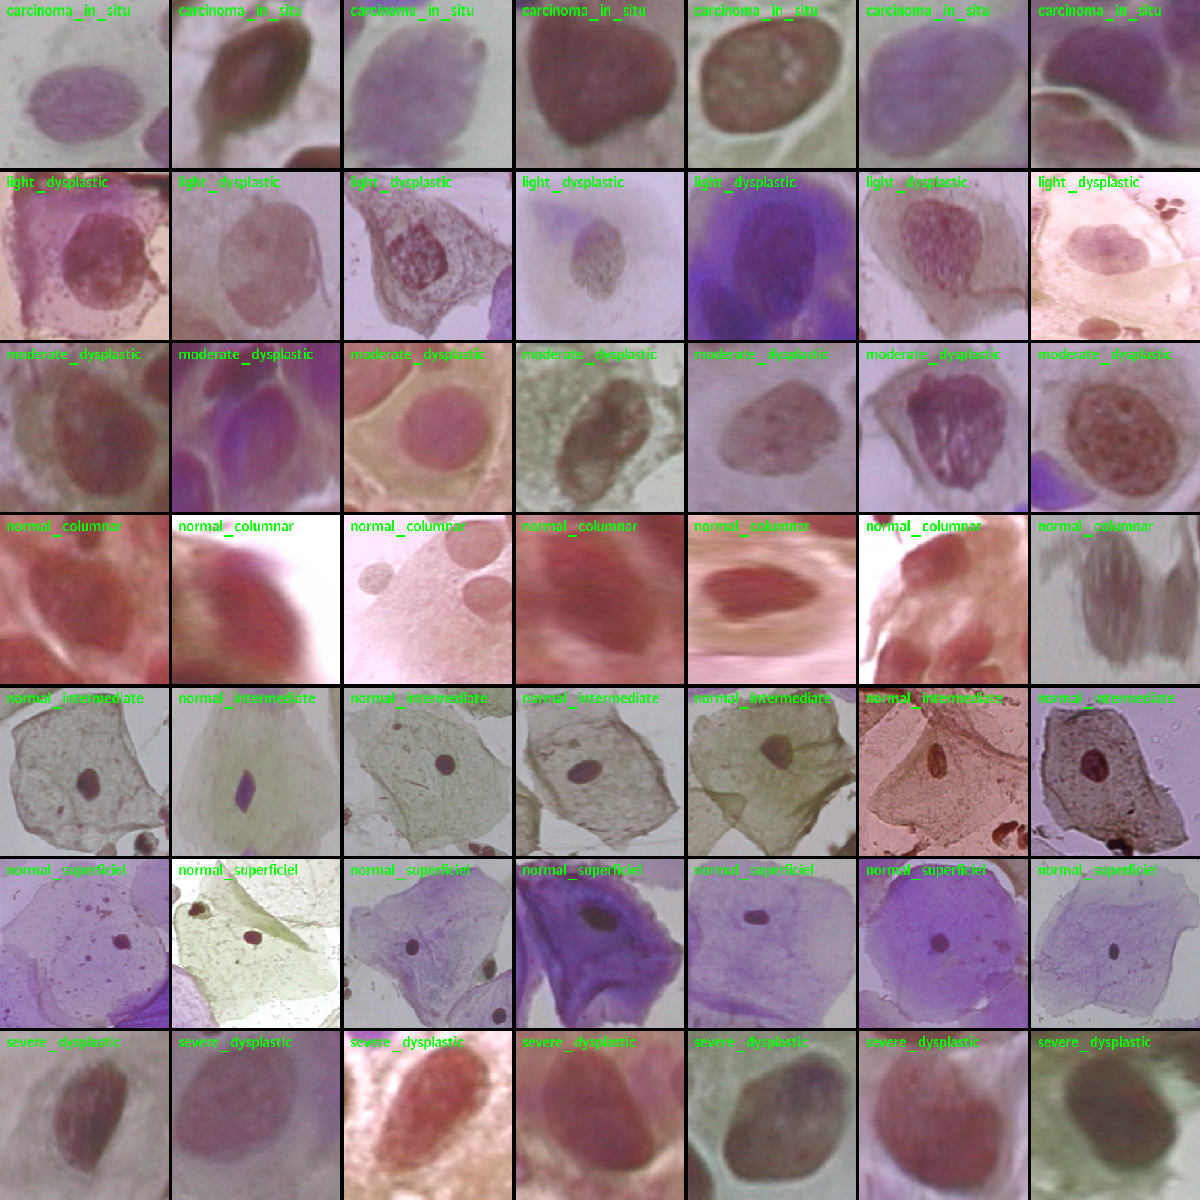
\includegraphics[width=1\textwidth]{capitulo_sdac/muestras_celulas}
    \caption{Muestreo de la BD}\label{fig:muestras_celulas}
\end{figure}

\begin{figure}[]
    \centering
    \includegraphics[width=1\textwidth]{capitulo_sdac/muestras_mascaras}
    \caption{Muestreo de la BD}\label{fig:muestras_mascaras}
\end{figure}

\subsection{Identificar transformaciones}

En esta esta debemos identificar transformación aplicables: Estas
transformaciones pueden incluir transposición matricial, cambio de espacio de
color, cambio en la escala de tiempo, etcétera.

Para datos tabulares, se pueden aplicar transformaciones para cambiar la escala
de los datos y restringirlos a valores pequeños para facilitar el aprendizaje
del modelo. Normalizar se refiere a restringir los datos a una escala entre 0 y
1. Estandarizar resta la media y divide por la varianza.

\subsubsection{Transformaciones aplicables a imágenes}

Transformaciones en imágenes incluyen normalizar pixeles a un rango entre 0 y 1, dividiendo
entre 255 la intensidad de cada pixel (\autoref{eq:pixel_norm}).

\begin{equation}
    \label{eq:pixel_norm}
    I_{norm} = I_{p} / 255
\end{equation}

En nuestro caso, las imágenes celulares tienen dos tipos de simetría. La
simetría axial es, dado cierto eje, podemos reflejar la imagen y seguirá siendo
simétrica. La simetría radial, es dado un punto, podremos rotar la imagen sobre
él sin que pierda su propiedad de simetría.

\begin{figure}[H]
    \centering
    \includegraphics[width=0.7\textwidth]{capitulo_sdac/simetrias}
    \caption{Tipos de simetría}\label{fig:simetrias}
\end{figure}

La normalización nos ayudará a entrenar la \hyperlink{abbr}{ConvNet}, reduciendo la libertad de
valores que puede tomar cada peso dentro de la red. Mientras que las
transformaciones de simetría nos ayudarán en la fase de aumento para generar más
datos e incrementar el poder de generalización del modelo.

\subsection{Información}

Al finalizar este proceso, habremos generado información pertinente que nos
ayudará a pre-procesar los datos para su posterior entrenamiento. Sabemos
cuantos datos tenemos y de que clase, información estadística de la \hyperlink{abbr}{BD}, como
es cada dato individual y las transformaciones que se le pueden aplicar al mismo.

Ya que la imagen contiene la célula y su máscara, pero no contiene las
coordenadas de cada objeto dentro de la imagen o imágenes con múltiples objetos,
podremos aplicar clasificación y segmentación semántica pero no detección ni
instanciación. Esto nos da un indicio de los algoritmos y arquitecturas a utilizar.

Finalmente, aumentaremos el archivo de excel que encontramos dentro de la
carpeta de la \hyperlink{abbr}{BD} de la siguiente manera
(\autoref{tabla:ananidas}). Este archivo servirá como inicio para los algoritmos
posteriores de pre-procesamiento. 

% Please add the following required packages to your document preamble:
% \usepackage{booktabs}
% \usepackage{graphicx}
\begin{table}[H]
    \centering
    \resizebox{0.5\textwidth}{!}{%
    \begin{tabular}{@{}ll@{}}
    \toprule
    Columna & Descripcion \\ \midrule
    Class\_cat\_2 & Clase categórica binaria \\
    Class\_num\_2 & Clase numérica binaria \\
    Class\_cat\_7 & Clase categórica multi-clase \\
    Class\_num\_7 & Clase numérica multi-clase \\
    file & Dirección absoluta de la imagen \\
    file\_masks & Dirección absoluta de la máscara \\ \bottomrule
    \end{tabular}%
    }
    \caption{Columnas añadidas al archivo}\label{tabla:ananidas}
    \end{table}



\section{Preprocesamiento}
Como se mencionó anteriormente, esta fase difiere entre el \hyperlink{abbr}{ML}
tradicional y el \hyperlink{abbr}{DL}. Mientras que en el primero nos enfocamos
a datos tabulares que tienen a ser abundantes, en el segundo nos comprometemos a
trabajar con pocos datos; por lo que la fase de preprocesamiento se enfocará más
a aumentar la base de datos, balancear las clases que la componen y lidiar con
detalles técnicos en la manipulación de vectores, matrices y tensores.

Debido a que en esta tesis trabajaremos con datos en imágenes y aplicamos
\hyperlink{abbr}{ConvNet}s que son capaces de aprender las características
importantes por si solas, podremos saltarnos las fases de ingeniería y selección
de características.

\subsection{Limpieza de datos}

Los archivos que contienen los datos y los procesos que generan los datos
también pueden incidir en ruido. Limpiar los datos se refiere a rellenar valores
faltantes utilizando técnicas de imputación de datos, estandarización y
normalización y también la remoción de valores inusuales.

En nuestro caso, debido a que la \hyperlink{abbr}{BD} esta pre-validada. No es
necesario limpiar los datos.

\subsection{Ingeniería de características}

Las tareas dentro de la Ingeniería de Características son: Discretizar valores
continuos, descomposición de atributos (categóricos, fechas y tiempos), aplicar
transformaciones (logarítmicas, raíces cuadradas y potencias), generar
atributos compuestos con datos correlacionados y no correlacionados.

También lo es el \emph{One-Hot Encoding}, que es transformar un dato categórico
en un vector de \( n \) elementos donde n es cada clase (\autoref{fig:onehot}).
Esta es la única técnica de ingeniería que usaremos en nuestros modelos, ya que
usaremos la función SoftMax.

\begin{figure}[H]
    \centering
    \includegraphics[width=0.5\textwidth]{capitulo_sdac/one-hot-encoding}
    \caption{Ejemplo de \emph{One-Hot Encoding}}\label{fig:onehot}
\end{figure}

\subsection{Selección de características}

Seleccionar los atributos, columnas en datos tabulares, importantes para
resolver el problema, involucra tanto conocimiento del dominio como técnico.
Elegir las mejores características asegurará que el modelo aprenda correctamente
para solucionar el problema. Difiere de la reducción de dimensionalidad en que
esta crea nuevas combinaciones de atributos para crear nuevas columnas, mientras
que la selección excluye atributos.

\subsection{Aumentación}

Para aumentar la \hyperlink{abbr}{BD} sacaremos parches de \(m \times m\),
centrados en el núcleo y rotaremos la célula un número fijo de grados. Para
encontrar el núcleo, nos auxiliaremos de la máscara para extraer el centroide de
la región del núcleo; luego exportaremos esas coordenadas a la imagen normal
para ser rotada. Para balancear la \hyperlink{abbr}{BD}, generaremos más parches
para las células normales que para las anormales. El \emph{DataFrame} es la
representación programática de una tabla de excel o archivo csv, con la mista
estructura tabular (\autoref{alg:aumentacion}). 

\begin{algorithm}[H]
    \SetAlgoLined{}
    \SetKwInOut{Input}{Input}\SetKwInOut{Output}{Output}
    \Input{Dataframe de imágenes}
    \Output{Imágenes aumentadas}
    \(m \longleftarrow 128\)
    \BlankLine{}
    \(balance \longleftarrow 0\)
    \BlankLine{}
    \For{\(row \in df\)}{    
        \BlankLine{}
        \(imagen \longleftarrow open(row[''file''])\)
        \BlankLine{}
        \uIf{\(row[''Class\_cat\_2''\)] == normal}{
            \(balance = 50\)
        }
        \uElse{
            \(balance = 18\)
        }
        \For{\(angle \in sample(balance)\)}{
            \BlankLine{}
            \(rot \longleftarrow rotate\_bound(imagen, angle)\)
            \BlankLine{}
            \(x, y \longleftarrow centro(rot)\)
            \BlankLine{}
            \(random = randint(5, 10)\)
            \BlankLine{}
            \(salida = sub\_image(rot, (x,y), angle, m, m, desp=random)\)
            \BlankLine{}
            \(salida = resize(salida, (256, 256))\)
            \BlankLine{}
        } 
    }
    \caption{Algoritmo para aumentación de datos}\label{alg:aumentacion}
\end{algorithm}

Se tomaron 50 muestras para células normales y 18 muestras para anormales de un
rango de ángulos entre 0 y 360 grados. Posteriormente se extrajo el centroide de
la imagen usando la máscara\footnote{Utilizando una técnica llamada Método de
Momentos.}. Los parches fueron extraídos de estas imágenes rotadas, la medida fue
de \(128 \times 128\) pixeles y, para asegurar cierta variación para hacer el
modelo más robusto, se desplazó el centro en el eje \(x\) y \(y\) por un número
aleatorio entre 5 y 10 pixeles. Por último se cambió el tamaño de la imagen a
\(256 \times 256\) pixeles (\autoref{fig:muestras_augment}). 
  
\begin{figure}[H]
    \centering
    \includegraphics[width=0.5\textwidth]{capitulo_sdac/muestras_augment}
    \caption{Muestreo de la BD aumentada (células)}\label{fig:muestras_augment}
\end{figure}

No solo se aumentaron las imágenes de células normales, sino también las de las
máscaras (\autoref{fig:muestras_augment_masks}). Bajo el contraste de la máscara
podemos apreciar cómo las células normales presentan más regularidad en sus
estructuras y las anormales se vuelven más caóticas.

\begin{figure}[H]
    \centering
    \includegraphics[width=0.5\textwidth]{capitulo_sdac/muestras_augment_masks}
    \caption{Muestreo de la BD aumentada (máscaras)}\label{fig:muestras_augment_masks}
\end{figure}

\subsection{Conocimiento}

Como conocimiento, tenemos una BD con imágenes variadas y aumentadas
aleatoriamente capaz de maximizar el poder de generalización de nuestro
algoritmo. Una preocupación que incluimos en el supuesto, es la de si la fase de
aumentación de datos incide en la capacidad de decisión del algoritmo. Esto es
evidente en las imágenes aumentadas, donde las partes que se añaden a la imagen
en el proceso de rotación y de cambio de tamaño se llenan con pixeles negros. 

Finalmente generamos un archivo \emph{.csv} con todas las imágenes aumentadas y su ruta
absoluta. Esto nos permitirá entrenar el modelo sin cargar todas las imágenes la
memoria, algo que sería totalmente impráctico, haciendo uso de una función que
nos permite alimentar fila por fila el archivo al algoritmo de entrenamiento.


\section{Elección algorítmica}

Aquí se realizará una exploración general de soluciones para indagar su
efectividad, esta exploración va guiada por el conocimiento del dominio y del
experto para asegurar su aplicabilidad final. No es necesario buscar en todo el
espectro de modelos, por ejemplo, el análisis de lenguaje natural se puede
resolver eficazmente con las Redes Neuronales,  gracias a esto el universo a
explorar será de arquitecturas. Esta fase puede ser muy intensiva
computacionalmente, así que la cantidad de iteraciones está limitada, como ya
sabemos el problema radica en que no existe una forma de determinar que modelo
será el mejor para un problema en particular.

En nuestro caso, ya hemos delimitado el tipo de algoritmo a utilizar. Si se
tiene \hyperlink{abbr}{BD} tabular, se procedería a: Probar modelos lineales,
bayesianos, Máquinas de Soporte Vectorial, Árboles Aleatorios, Redes Neuronales
y demás, usando parámetros estándar para estimar su rendimiento.

Para cada modelo, es preferible utilizar una validación cruzada y comparar tanto
la media como la desviación estándar. En algoritmos como las
\hyperlink{abbr}{ConvNet}s, esto puede ser difícil debido a la complejidad
computacional\footnote{Los tiempos por época llegan a ser de entre 5 y 10
minutos, cada iteración puede tener hasta 50 épocas.}. También lo es determinar
el tipo de error estadístico de cada modelo para corroborar el impacto que
tendrá tal error en el rendimiento del algoritmo en situaciones de la vida real,
por ejemplo, en el área médica es importante la tasa de falsos positivos y
falsos negativos.

Este proceso es naturalmente iterativo. Donde cambios en algoritmos,
arquitecturas e hiperparámetros obviamente modifican el rendimiento de los
algoritmos. El objetivo es encontrar un subconjunto muy reducido de candidatos a
probar, ya que estamos limitados por el tiempo y la complejidad computacional de
algunos modelos, que inclusive llegan a tardar semanas en entrenarse.

\subsection{Probar distintos algoritmos}

Se han probado varias arquitecturas desde las más grandes hasta las más
eficientes, todas ellas implementadas en lenguaje Python utilizando
\textbf{Keras}. El \emph{Zoológico de Modelos} es el término que engloba
arquitecturas de \hyperlink{abbr}{ConvNet}s pre-entrenadas para diversas tareas
de \hyperlink{abbr}{VC} (\emph{ImageNet}) y por lo general se manejan con
licencias libres, lo cual permite su implementación para resolver tanto
problemas generales como particulares si se aplica \hyperlink{abbr}{TL}.

La elección de estos algoritmos está basada directamente en la elección del
software utilizado para el desarrollo. Por lo que nos enfocaremos en el
\emph{Zoológico de Modelos} de \textbf{Keras} y su \emph{backend}:
\textbf{TensorFlow}\footnote{Anteriormente Keras era capaz de trabajar con
Theano como \emph{Backend}.}. Para la búsqueda del mejor candidato a modelo solución se
realizó un experimento de búsqueda exhaustiva por todo el espacio de soluciones
comprendido dentro del \emph{Zoológico de Modelos} de \textbf{Keras}. Para ello
se programó un script automatizado que alimenta el ciclo de entrenamiento con
cada modelo de este espacio y captura los resultados del entrenamiento por
época, así como las métricas como la pérdida y la exactitud de cada iteración
del experimento.

\subsubsection{Arquitecturas probadas}

Las arquitecturas probadas fueron las siguientes y serán entrenadas con los
mismos hiperparámetros y el mismo número de épocas
(\autoref{fig:hiper_transfer}):

\begin{enumerate}
    \item DenseNet201
    \item InceptionResNetV2
    \item InceptionV3
    \item MobileNet
    \item MobileNetV2
    \item NASNetLarge
    \item NASNetMobile
    \item ResNet50
    \item VGG16
    \item VGG19
    \item Xception
\end{enumerate}

\begin{figure}[H]
    \centering
    \begin{minted}{python}
                        BATCH_SIZE = 64
                        FC_LAYERS = [1024, 1024]
                        LR = 0.00001
                        OPT = Adam(lr=LR)
                        EPOCHS = 20
                        DROPOUT = 0.5
    \end{minted}
    \caption{Hiperparámetros para búsqueda de algoritmos}\label{fig:hiper_transfer}
\end{figure}

\subsection{Comparar rendimiento}

Los resultados de los experimentos, sus gráficas, tablas y por arquitectura se
muestran en el \autoref{appendix:comparativa}. También incluye una breve
interpretación individual para cada arquitectura y el comportamiento de sus
métricas tanto en entrenamiento como en validación.

\subsection{Analizar métricas}

El análisis de las exactitudes de las arquitecturas probadas tanto en validación
como en entrenamiento se muestra en la~\autoref{fig:comp_total}. Podemos ver que
el comportamiento en entrenamiento fue bastante similar en todas las redes. Esto
cambió drásticamente en la fase de validación, donde la familia VGG se destacó
por sobre todas las demás. Así como en la exactitud, la pérdida se comportó
bastante similar en todos los modelos en la fase de entrenamiento. En
la~\autoref{fig:comp_totalloss} se muestra que algunas arquitecturas se
comportaban peor al pasar las épocas.

\begin{figure}[H]
    \centering
    \begin{subfigure}[b]{0.8\textwidth}
        \centering
       \includegraphics[width=1\textwidth]{capitulo_sdac/exactitud_entrenamiento.pdf}
       \caption{Exactitud en entrenamiento}\label{fig:comp_ent} 
    \end{subfigure}

    \begin{subfigure}[b]{0.8\textwidth}
        \centering
       \includegraphics[width=1\textwidth]{capitulo_sdac/exactitud_validacion.pdf}
       \caption{Exactitud en validación}\label{fig:comp_val}
    \end{subfigure}
    \caption{Gráfica de comparativa de exactitud}\label{fig:comp_total}
\end{figure}
\begin{figure}[H]
    \centering
    \begin{subfigure}[b]{0.8\textwidth}
        \centering
       \includegraphics[width=1\textwidth]{capitulo_sdac/perdida_entrenamiento.pdf}
       \caption{Pérdida en entrenamiento}\label{fig:comp_entloss} 
    \end{subfigure}

    \begin{subfigure}[b]{0.8\textwidth}
        \centering
       \includegraphics[width=1\textwidth]{capitulo_sdac/perdida_validacion.pdf}
       \caption{Pérdida en validación}\label{fig:comp_valloss}
    \end{subfigure}
    \caption{Gráfica de comparativa de pérdida}\label{fig:comp_totalloss}
\end{figure}

\subsection{Seleccionar los mejores algoritmos}

Una vez terminado el proceso de entrenamiento se requiere crear una lista con
los mejores modelos, teniendo siempre en mente la aplicabilidad final del
algoritmo. Pueden existir algoritmos con mejor rendimiento que por sus
características los hacen imposibles de implementar en el área donde surge el
problema. Por ejemplo, las \hyperlink{abbr}{RNA} son restrictivas en su
aplicación y prefieren ser desplegadas en sistemas donde se tenga disponible un
\hyperlink{abbr}{GPU} para realizar los cálculos.

\subsubsection{Algoritmo ganador}

Claramente los ganadores son las arquitecturas VGG16 y VGG19 entrenadas con
\emph{ImageNet}, alcanzando esta última una mejor exactitud en el mismo número
de épocas. Sabemos que esta arquitectura es suficientemente ligera para ser
implementada tanto en dispositivos móviles como en sistemas embebidos, en dado
caso que su tamaño impida una implementación con un rendimiento adecuado, se
puede optar por utilizar la VGG16 por su menor tamaño. Descubrir la razón por la
cual algunas arquitecturas se comportaban pésimo durante el experimento está
fuera del espectro de esta tesis, así como la búsqueda de otros modelos que
puedan resultar aptos y no estén implementados en \textbf{Keras} como las otras
arquitecturas de ResNet o CaffeNet.

Para segmentación semántica, solamente probaremos un algoritmo: Unet, ya que por
sus características, debido a las restricciones de tiempo y a su rendimiento
probado en aplicaciones citológicas, es claramente la mejor arquitectura para
este experimento. Esta arquitectura no implementará \hyperlink{abbr}{TL}. 

\subsection{Experimento}

Teniendo las arquitecturas o algoritmos ganadores, se puede diseñar un
experimento. El cual realizarse con todas las disposiciones
estadísticas para estimar correctamente el rendimiento del algoritmo en cada
iteración del proceso. El experimento consistirá en cambiar los hiperparámetros
del algoritmo para encontrar los mejores y asegurar un mejor rendimiento.
Existen distintas maneras de realizar este proceso pero están fuera del espectro
de esta tesis.

Al realizar el experimento, debemos de tener especial atención en guardar
absolutamente todos los cambios que se hagan tanto al algoritmo como a los
hiperparámetros, para poder analizar correctamente el rendimiento del modelo. El experimento
debe tener las siguientes características~\cite{Broman2017}:

\begin{enumerate}
    \item{\textbf{Repetible:}} Es la capacidad de volver a hacer el experimento
    en otro entorno ajeno al del investigador original y con un código
    independiente al entorno inicial de investigación.
    \item{\textbf{Reproducible:}} Un estudio es reproducible si se pueden tomar
    los datos originales y el código computacional usado para analizarlos y
    reproducir todos los hallazgos numéricos del estudio.
    \item{\textbf{Replicable:}} Es el acto de repetir un estudio completo,
    independientemente del investigador original sin el uso de datos originales
    y utilizando los mismos métodos.
\end{enumerate}

\section{Ajustar modelo}
Ajustar y optimizar es un proceso iterativo susceptible a la automatización.
Esta fase se refiere a la búsqueda de arquitectura (tamaño de las capas, número
de neuronas) e hiperparámetros (tamaño de lote, tasa de aprendizaje) que harán
que el modelo elegido en la fase anterior alcance su mayor potencial y
posiblemente solucione el problema. Cabe mencionar que todos estos pasos no
garantizan converger a una solución específica, y puede que se tenga que pasar
por varias iteraciones de la metodología para encontrar alguna satisfactoria.

Los hiperparámetros pueden ser exclusivos para cada algoritmo, sin embargo, las
técnicas de búsqueda de hiperparámetros son universales (Búsqueda reticular,
búsqueda aleatoria, bayesiana, metaheurísticas). Si los recursos computacionales
lo permiten, utilizar ensamblaje de modelos es mejor que un solo modelo.

Al ser la fase más computacionalmente intensiva de toda la metodología, esta
fase tiende a ser tardada, normalmente de muchas horas. Al finalizar tendremos
no solo el mejor modelo, sino una evaluación del mismo que nos permitirá avanzar
a la culminación del proceso, o comenzar el proceso una vez más si el
rendimiento no es satisfactorio.

Se procederá realizar tres experimentos. Cada uno de ellos será entrenado por el
mismo algoritmo de entrenamiento y tendrá sus hiperparámetros particulares y se
someterán a varias pruebas y validaciones:

\begin{enumerate}
    \item{\textbf{Clasificación binaria:}} Clasificar las imágenes citológicas
    en normales y anormales.
    \item{\textbf{Clasificación multi-clase:}} Clasificar las imágenes en las
    siete clases del sistema \emph{Bethesda}. Esta será el modelo que llegará a
    la solución final y por ello es el que lleva mayor cantidad de análisis.
    \item{\textbf{Segmentación semántica:}} Segmentar cada pixel de la imagen
    citológica en dos clases: núcleo o el resto (citoplasma o fondo).
\end{enumerate}

\subsection{Implementar validación cruzada}

Se cuenta con un archivo .csv que concentra la ruta de la imagen, la clase y la
categoría a la que pertenece. Implementar validación cruzada se reduce a dividir
aleatoriamente los índices de cada fila de tal archivo. Para ello se utilizará
el módulo \emph{Pandas} para manejar los datos tabulares para implementar la
validación cruzada mediante el módulo \emph{Sklearn} y su función
\mintinline{latex}{Kfold}.

La fase de segmentación semántica no cuenta con gráfica de validación cruzada ya
que no se dividen las imágenes por clases.

Se decidió una \mintinline{latex}{K = 10} ya que tienen el mejor compromiso
entre sesgo y varianza. Este proceso es muy tardado pero para asegurar una
estimación precisa del error de generalización, se decidió que era la mejor
opción para validar este trabajo.

\subsubsection{Clasificación binaria}

En la~\autoref{fig:kfold} se representa la planeación de la validación cruzada,
las dos clases, sus índices y como el algoritmo escoge aleatoriamente
subconjuntos (índices) aleatoriamente en cada iteración, para asegurar una
correcta validación del algoritmo. Se decidió por 10 iteraciones debido a la
complejidad computacional, tardando esta fase 22 horas en completarse.

\begin{figure}[H]
    \centering
    \includegraphics[width=0.9\textwidth]{capitulo_sdac/kfold_10_2.png}
    \caption{Kfold de 10 iteraciones binario}\label{fig:kfold}
\end{figure}

\subsubsection{Clasificación multi-clase}

La~\autoref{fig:kfold_7} muestra la validación cruzada aplicada al problema de 7
clases. Existe discrepancia en la cantidad de elementos por cada una de las
clases, es decir, es un entrenamiento desbalanceado y procederemos a evaluar el
impacto de ello en el experimento. Este entrenamiento fue sumamente tardado: 44
horas, ya que duplicamos el número de épocas de entrenamiento.

\begin{figure}[H]
    \centering
    \includegraphics[width=0.9\textwidth]{capitulo_sdac/kfold_10_7.png}
    \caption{Kfold de 10 iteraciones multi-clase}\label{fig:kfold_7}
\end{figure}

\subsection{Elegir hiperparámetros}

Una correcta elección de hiperparámetros asegura que el modelo convergerá para
dar solución al problema. Si elegimos mal puede hacer que el algoritmo jamás
funcione o tenga un comportamiento errático. 

\begin{itemize}
    \item El tamaño de lote o \mintinline{latex}{BATCH_SIZE} se dejó como máximo
    en $64$. Más grande hacía que el \hyperlink{abbr}{GPU} se quedara sin
    memoria antes de terminar.
    \item Las neuronas de la capa densa o totalmente conectada
    \mintinline{latex}{FC_LAYERS} se dejan en $1024$ neuronas en comparación a
    las $4096$ que tiene VGG original.
    \item Como optimizador \mintinline{latex}{OPT} se eligió Adam y este cuenta
    con solo un hiperparámetro \mintinline{latex}{LR} que es la tasa de
    aprendizaje. Para \hyperlink{abbr}{TL} se prefieren tasas pequeñas.
    \item \mintinline{latex}{DROPOUT} define la probabilidad de apagar una
    neurona particular en las capas densas y generalmente se sitúa en $50\%$.
\end{itemize}

\subsubsection{Clasificación binaria}

Los hiperparámetros usados para el entrenamiento del modelo se muestran a
continuación. La variable global \mintinline{latex}{KFOLD_SPLITS} determina la
cantidad de iteraciones en la validación cruzada, lo cual nos permite evaluar el
rendimiento del algoritmo con la mayor exactitud posible y con las mejores
prácticas estadísticas (\autoref{fig:hiper_dosclases}).

\begin{figure}[H]
    \centering
    \begin{minted}{python}
                            BATCH_SIZE = 64
                            FC_LAYERS = [1024, 1024]
                            LR = 0.00001
                            OPT = Adam(lr=LR)
                            EPOCHS = 30
                            DROPOUT = 0.5
                            KFOLD_SPLITS = 10
    \end{minted}
     \caption{Hiperparámetros para dos clases}
     \label{fig:hiper_dosclases}
\end{figure}

\subsubsection{Clasificación multi-clase}

A continuación se muestran los hiperparámetros utilizados, se incrementó la tasa
de aprendizaje y se duplicó el numero de épocas debido a la mayor complejidad
del problema  (\autoref{fig:hiper_sieteclases}), debido a esto el experimento
tardó el doble en completarse como era lógico:

\begin{figure}[H]
    \centering
\begin{minted}{python}
                            BATCH_SIZE = 64
                            FC_LAYERS = [1024, 1024]
                            LR = 0.0001
                            OPT = Adam(lr=LR)
                            EPOCHS = 60
                            DROPOUT = 0.5
                            KFOLD_SPLITS = 10
\end{minted}
\caption{Hiperparámetros para siete clases}
\label{fig:hiper_sieteclases}
\end{figure}

\subsubsection{Segmentación semántica}

Los hiperparámetros usados en el experimentos son los siguientes, notar que el
optimizador usa los valores por defecto que recomienda \textbf{Keras}. Se redujo
\mintinline{latex}{BATCH_SIZE} a la mitad ya que en realidad estamos pasando dos
imágenes por cada iteración de entrenamiento en lugar de una
(\autoref{fig:hiper_segmentacion}). Para este experimento nos conformaremos con
solo cinco iteraciones ya que los previos tardaron mucho:

\begin{figure}[H]
    \centering
\begin{minted}{python}
                            BATCH_SIZE = 32
                            LR = 0.001
                            OPT = Adam(lr=LR)
                            EPOCHS = 50
                            DROPOUT = 0.5
                            KFOLD_SPLITS = 5
\end{minted}
\caption{Hiperparámetros para segmentación semántica}
\label{fig:hiper_segmentacion}
\end{figure}

\subsection{Entrenar modelo}

Una vez encontrado el mejor modelo, procederemos a aplicar Fine-Tuning y la
optimización de hiperparámetros. La última capa del modelo pre-entrenado fue
removida y reemplazada por una capa densa totalmente conectada, para luego ser
entrenada en conjunto a toda la red. Convirtiendo un modelo general en un
predictor particular, capaz de clasificar células en distintas clases.

El ciclo de entrenamiento (\autoref{alg:entrenamiento}) es general para los tres
experimentos. Recibe como entrada una BD representada por un archivo .csv
cargado a memoria como dataframe y como salida da el mejor modelo. La variable
\mintinline{latex}{results} es una lista que va a guardar el rendimiento de cada
modelo entrenado en cada iteración \mintinline{latex}{k = 5}. La función
\mintinline{latex}{Kfold} divide los datos y devuelve \mintinline{latex}{j,
train, val} que son el índice de la iteración, los índices de entrenamiento y
los índices de validación. Se construye el modelo pasando los hiperparámetros a
la función \mintinline{latex}{build_model}. Se guarda el resultado de ajustar el
modelo por el número de épocas. El error de generalización es el promedio del
rendimiento de todos los resultados y se escoge el mejor modelo con la función
\mintinline{latex}{best_index} que devuelve el índice del elemento más grande en
la lista \mintinline{latex}{results}.

\begin{algorithm}[H]
    \SetAlgoLined
    \SetKwInOut{Input}{Input}\SetKwInOut{Output}{Output}
    \Input{Database}
    \Output{Best model}
    $results \longleftarrow [ ... ]$
    \BlankLine
    $models \longleftarrow [ ... ]$
    \BlankLine
    $batch\_size \longleftarrow 128$
    \BlankLine
    $epochs \longleftarrow 50$
    \BlankLine
    $layers \longleftarrow [1024, 1024]$
    \BlankLine
    $opt \longleftarrow Adam$
    \BlankLine
    $lr \longleftarrow 1e-4$
    \BlankLine
    $dropout \longleftarrow [0.5, 0.5]$
    \BlankLine
    $k \longleftarrow 5$
    \BlankLine
    $\mathbb{D}  \longleftarrow database$
    \BlankLine
    \For{$j, train, val \in Kfold(splits=k, data=\mathbb{D})$}{    
        \BlankLine
        $model = build\_model(dropout, layers, opt(lr))$
        \BlankLine
        $result = model.fit(train, epochs)$
        \BlankLine
        $models[j] \longleftarrow model$
        $results[j] \longleftarrow result.evaluate(val)$
    }
    \BlankLine
    $generalization\_error \longleftarrow mean(results)$
    \BlankLine
    $best\_model\_idx \longleftarrow best_index(results)$
    \BlankLine
    $best\_model = models[best\_model\_idx]$
    \caption{Ciclo de entrenamiento}\label{alg:entrenamiento}
\end{algorithm}

Las tablas de rendimiento por época para los tres experimentos se pueden
encontrar en el \autoref{appendix:entrenamiento}.

\subsubsection{Clasificación binaria}

La~\autoref{tabla:rendimiento:final} nos muestra como se comportó el modelo
en las 30 épocas de entrenamiento tanto en entrenamiento como en validación. Es
clara la tendencia del algoritmo a mejorar con respeto a las épocas, aunque se
sigue notando cierta discrepancia entre los valores de validación y
entrenamiento, queremos que estos valores sean lo más cercanos posibles.

Los resultados de la validación cruzada se pueden observar el
la~\autoref{tabla:validacion}. La iteración con mejor rendimiento fue la número
6, alcanzando una exactitud del 99.91\%.

% Please add the following required packages to your document preamble:
% \usepackage{booktabs}
% \usepackage{graphicx}
\begin{table}[H]
    \centering
    \resizebox{0.4\textwidth}{!}{%
    \begin{tabular}{@{}lll@{}}
    \toprule
    fold & acc & loss \\ \midrule
    0 & 99.84536171 & 0.004982506 \\
    1 & 99.85566735 & 0.00357472 \\
    2 & 99.86597896 & 0.004019101 \\
    3 & 99.89690781 & 0.003187174 \\
    4 & 99.8865962 & 0.00304257 \\
    5 & 99.8865962 & 0.004015994 \\ \midrule
    6 & 99.91752505 & 0.002261744 \\ \midrule
    7 & 99.87629056 & 0.002811817 \\ 
    8 & 99.77319837 & 0.006879645 \\
    9 & 99.82474446 & 0.00390799 \\ \bottomrule
    \end{tabular}%
    }
    \caption{Resultados de la validación cruzada binaria}
    \label{tabla:validacion}
    \end{table}

La~\autoref{tabla:estadisticos} concluye el experimento, la exactitud final
alcanzada es el promedio de las iteraciones: $99.86\% \pm 0.0412$. Un
rendimiento bastante aceptable, siendo el error de generalización del modelo un
total de $0.14\%$.

\begin{table}[H]
    \centering
    \resizebox{0.4\textwidth}{!}{%
    \begin{tabular}{@{}lll@{}}
    \toprule
     & acc & loss \\ \midrule
    count & 10 & 10 \\
    mean & 99.86288667 & 0.003868326 \\
    std & 0.041250406 & 0.001303197 \\
    min & 99.77319837 & 0.002261744 \\
    25\% & 99.84793812 & 0.003078721 \\
    50\% & 99.87113476 & 0.003741355 \\
    75\% & 99.8865962 & 0.004018324 \\
    max & 99.91752505 & 0.006879645 \\ \bottomrule
    \end{tabular}%
    }
    \caption{Estadísticos del experimento binario}
    \label{tabla:estadisticos}
    \end{table}

A continuación se mostrarán las métricas de la mejor iteración, que nos ofrecerá
información sobre el comportamiento del experimento y de su rendimiento. Las
métricas cuentan con su gráfica normal y una aplicando suavizado exponencial
para mejorar su interpretación.

La pérdida durante el entrenamiento y validación se muestran en
la~\autoref{fig:perdida_total}, donde la tendencia a disminuir es clara,
estabilizándose alrededor de la época número 15.

\begin{figure}[H]
    \centering
    \includegraphics[width=0.7\textwidth]{capitulo_sdac/reporte_2_class/loss.pdf}
    \caption{Pérdida binaria}\label{fig:perdida_total}
\end{figure}

La exactitud se estabiliza alrededor de la época 15 como se muestra en
la~\autoref{fig:precision_total}. Se detecta que tanto en la pérdida como en la
exactitud que ambas curvas se acercan la una a la otra, lo que nos dice que el
modelo está ajustado de manera excelente.

\begin{figure}[H]
    \centering
    \includegraphics[width=0.7\textwidth]{capitulo_sdac/reporte_2_class/acc.pdf}
    \caption{Precisión binaria}\label{fig:precision_total}
\end{figure}
    
\subsubsection{Clasificación multi-clase}

La~\autoref{tabla:rendimiento_7} nos permite ver que el algoritmo incrementa su
rendimiento al pasar las épocas, aunque cada vez se le hace más difícil mejorar
sus métricas. Quizás se puedan implementar acciones que optimicen los
hiperparámetros o inclusive técnicas de entrenamiento adaptativas o quizás
probar con otro optimizador.

Los resultados de la validación cruzada de 10 iteraciones para el experimento
multi-clase se ven en la~\autoref{tabla:validacion7}. La iteración con mejor
rendimiento fue la número 1, alcanzando una exactitud del 99.72\%. Se manifiesta
cierto fenómeno donde la pérdida de la iteración 0 es mejor que la 1. Esto puede
ser debido a fluctuaciones del generador de números aleatorios.

\begin{table}[H]
    \centering
    \resizebox{0.4\textwidth}{!}{%
    \begin{tabular}{@{}lll@{}}
    \toprule
    fold & acc & loss \\ \midrule
    0 & 99.69072342 & 0.009913217 \\ \midrule
    1 & 99.72165227 & 0.010205996 \\ \midrule
    2 & 99.59793687 & 0.013710575 \\
    3 & 99.49484468 & 0.014681551 \\
    4 & 99.49484468 & 0.016252176 \\
    5 & 99.60824847 & 0.0124342 \\
    6 & 99.60824847 & 0.011963185 \\
    7 & 99.57731962 & 0.014334826 \\
    8 & 99.46391582 & 0.016523478 \\
    9 & 99.62886572 & 0.013009808 \\ \bottomrule
    \end{tabular}%
    }
    \caption{Resultados de la validación cruzada multi-clase}
    \label{tabla:validacion7}
    \end{table}

La~\autoref{tabla:estadisticos7} concluye el experimento, la exactitud final
alcanzada es el promedio de las iteraciones: $99.58\% \pm 0.084$. Podemos ver
que tanto la especificidad como la sensibilidad tienen una desviación estándar
mayor que la exactitud, debido a la forma en que se calculan estas métricas. El
error de generalización total del modelo es de 0.42\%.

\begin{table}[H]
    \centering
    \resizebox{0.4\textwidth}{!}{%
    \begin{tabular}{@{}lll@{}}
    \toprule
     & acc & loss \\ \midrule
    count & 10 & 10 \\
    mean & 99.58866 & 0.013302901 \\
    std & 0.084239213 & 0.002258767 \\
    min & 99.46391582 & 0.009913217 \\
    25\% & 99.51546341 & 0.012080938 \\
    50\% & 99.60309267 & 0.013360192 \\
    75\% & 99.62371141 & 0.01459487 \\
    max & 99.72165227 & 0.016523478 \\ \bottomrule
    \end{tabular}%
    }
    \caption{Estadísticos del experimento multi-clase}
    \label{tabla:estadisticos7}
    \end{table}

La pérdida cayó abruptamente antes de las 10 épocas, después de las cuales se
estabilizó alcanzando cierto límite asintótico; Cuando se analiza la diferencia
entre la pérdida en entrenamiento y validación, estas se encuentran muy cercanas
y casi iguales lo cual es ideal, quiere decir que nuestro modelo puede capturar
muy bien las complejidades de la clasificación citológica multi-clase
(\autoref{fig:perdida_total_7}).

\begin{figure}[H]
    \centering
    \includegraphics[width=0.7\textwidth]{capitulo_sdac/reporte_7_class/loss.pdf}
    \caption{Pérdida con 7 clases}\label{fig:perdida_total_7}
\end{figure}

La exactitud del experimento multi-clase se comporta muy similar al del
experimento binario (\autoref{fig:precision_total_7}). Hay una mínima brecha
entre la metríca en entrenamiento y en validación probablemente se deba al
fenómeno de~\emph{underfitting}. Esto se podría solucionar reduciendo el
\mintinline{latex}{DROPOUT} o incrementando la complejidad del modelo, aunque la
diferencia es tan poca que puede no ser significativa.

\begin{figure}[H]
    \centering
    \includegraphics[width=0.7\textwidth]{capitulo_sdac/reporte_7_class/acc.pdf}
    \caption{Exactitud con 7 clases}\label{fig:precision_total_7}
\end{figure}


\subsubsection{Segmentación semántica}

En la segmentación semántica substituiremos las métricas de clasificación por la
Intersección sobre Union y la función de pérdida por el coeficiente de Dice, ya
que son las indicadas para arquitectura usada en este caso.

Los resultados de la validación cruzada para segmentación, con cinco
iteraciones, se compilan en la~\autoref{tabla:rendseg}, mientras que el resumen
y los estadísticos están en la~\autoref{tabla:estadisticosseg}. Claramente es la
primera iteración la que alcanzó los mejores resultados. Esta pérdida puede
tener valores negativos en comparación a la usada en las arquitecturas
anteriores. Si bien la exactitud es la métrica más alta, en este caso, la
correcta es IoU con un rendimiento total de 88.19\%.

\begin{table}[H]
    \centering
    \resizebox{0.5\textwidth}{!}{%
    \begin{tabular}{@{}llll@{}}
    \toprule
    fold & accuracy & loss & iou \\ \midrule
    0 & 91.0180247 & -0.896642793 & 0.884503568 \\ \midrule
    1 & 89.86388168 & -0.917515639 & 0.888006022 \\
    2 & 89.99839323 & -0.911953644 & 0.885471006 \\
    3 & 89.79965767 & -0.900890709 & 0.866708054 \\
    4 & 90.36797129 & -0.911352285 & 0.885264954 \\ \bottomrule
    \end{tabular}%
    }
    \caption{Rendimiento de la validación cruzada de segmentación}\label{tabla:rendseg}
    \end{table}

\begin{table}[H]
    \centering
    \resizebox{0.6\textwidth}{!}{%
    \begin{tabular}{@{}llll@{}}
    \toprule
    & accuracy & loss & iou \\ \midrule
    Número & 5 & 5 & 5 \\
    Media & 90.20958571 & -0.907671014 & 0.881990721 \\
    Desviación & 0.502696262 & 0.008608186 & 0.008644234 \\
    Mínimo & 89.79965767 & -0.917515639 & 0.866708054 \\
    25\% & 89.86388168 & -0.911953644 & 0.884503568 \\
    50\% & 89.99839323 & -0.911352285 & 0.885264954 \\
    75\% & 90.36797129 & -0.900890709 & 0.885471006 \\
    Máximo & 91.0180247 & -0.896642793 & 0.888006022 \\ \bottomrule
    \end{tabular}%
    } 
    \caption{Estadísticos del experimento}\label{tabla:estadisticosseg}
    \end{table}

La~\autoref{fig:perdida_seg} muestra los resultados de la pérdida en
entrenamiento y validación. Se pueden observar fluctuaciones considerables en
validación con una clara tendencia a estabilizarse conforme pasan las épocas de
entrenamiento.

\begin{figure}[H]
    \centering
    \includegraphics[width=0.7\textwidth]{capitulo_sdac/perdida_2.pdf}
    \caption{Gráfico de pérdida, se nota fluctuación en validación}\label{fig:perdida_seg}

\end{figure}

A continuación vemos (\autoref{fig:acc_total_seg}) la \emph{Intersection over
Union} en las dos fases. Se manifiesta una excelente curva que aumenta
constantemente en función de las épocas, reduciendo su incremento en cada
iteración pero siempre aumentando, igualmente, las dos curvas se mantienen muy
próximas entre si.

\begin{figure}[H]
    \centering
    \includegraphics[width=0.7\textwidth]{capitulo_sdac/exactitud_2.pdf}
    \caption{Gráfico de Intersección sobre Unión}\label{fig:acc_total_seg}

\end{figure}

\subsection{Evaluar modelo}

Para evaluar el modelo, primeramente haremos un análisis comparativo de las
métricas en validación y entrenamiento. En los problemas de clasificación, es
común realizar una gráfica conocida como Matriz de Confusión que nos permite ver
fácilmente la cantidad de elementos clasificados correcta o incorrectamente.
Aplicaremos un total de 22 métricas de evaluación para estimar, con la mayor
certeza posible, el rendimiento del modelo ya que su aplicación final será para
diagnóstico de cáncer.

Por último, tomaremos un muestreo de aquellas células que fueron mal
clasificadas, para poder observar las características morfológicas y apreciar
empíricamente los errores.

\subsubsection{Clasificación binaria}

Para determinar como difieren los valores de entrenamiento y validación, se
realizó una gráfica de caja con las métricas y la pérdida. La variabilidad
individual de estas métricas se muestra en la~\autoref{fig:caja_total2}. Se
aprecia que en la fase de entrenamiento, las métricas tienen una variabilidad
mayor, esto es debido a que la validación se hace siempre una época después que
el entrenamiento, por lo que esta se realiza con los pesos ya ajustados por la
función de pérdida, reduciendo su error total.

\begin{figure}[H]
    \centering
    \begin{subfigure}[b]{0.6\textwidth}
        \centering
        \includegraphics[width=1\textwidth]{capitulo_sdac/reporte_2_class/box_acc.pdf}
        \caption{Gráfico de caja de métricas}\label{fig:caja_acc2} 
    \end{subfigure}

    \begin{subfigure}[b]{0.6\textwidth}
        \centering
        \includegraphics[width=1\textwidth]{capitulo_sdac/reporte_2_class/box_loss.pdf}
        \caption{Gráfico de caja de pérdida}\label{fig:caja_loss2}
    \end{subfigure}
    \caption{Gráficos de caja binarios}\label{fig:caja_total2}
\end{figure}

La~\autoref{fig:caja_total} nos muestra la comparación de la variabilidad entre
la pérdida y la exactitud en validación, donde comprobamos efectivamente que su
variabilidad se reduce conforme pasan las épocas de entrenamiento y que el
modelo puede generalizar correctamente. Como ya sabemos, entre más cerca estén
las métricas, mejor.

\begin{figure}[H]
    \centering
    \begin{subfigure}[b]{0.6\textwidth}
        \centering
        \includegraphics[width=1\textwidth]{capitulo_sdac/reporte_2_class/variabilidad_acc.pdf}
        \caption{Variación en la exactitud}\label{fig:caja_acc} 
    \end{subfigure}

    \begin{subfigure}[b]{0.6\textwidth}
        \centering
        \includegraphics[width=1\textwidth]{capitulo_sdac/reporte_2_class/variabilidad_loss.pdf}
        \caption{Variación en la pérdida}\label{fig:caja_loss}
    \end{subfigure}
    \caption{Gráfica de caja de la variación binaria}\label{fig:caja_total}
\end{figure}

La~\autoref{tabla:reporte_2} nos muestra el reporte que evalúa un algoritmo de
clasificación, condensando la información básica por cada clase. Cabe notar que
los falsos positivos (FP) y falsos negativos (FN) son muy pocos comparados con
los datos utilizados para evaluar (POP). Las clases están desbalanceadas pero su
diferencia es una cantidad negligible. 

\begin{table}[H]
    \centering
    \resizebox{0.3\textwidth}{!}{%
    \begin{tabular}{@{}lll@{}}
    \toprule
    Class & anormal & normal \\ \midrule
    TP & 4899 & 4793 \\
    TN & 4793 & 4899 \\
    FP & 1 & 7 \\
    FN & 7 & 1 \\
    P & 4906 & 4794 \\
    N & 4794 & 4906 \\
    POP & 9700 & 9700 \\ \bottomrule
    \end{tabular}%
    }
    \caption{Reporte de clasificación binario}
    \label{tabla:reporte_2}
    \end{table}

La~\autoref{fig:matrices} nos muestra las matrices de confusión; la matriz
normalizada no se aprecia bien por el redondeo y se puede interpretar que el
sistema tiene un poder de clasificación perfecto, pero podemos ver en la matriz
no normalizada que un total de 8 elementos fueron mal clasificados, un ejemplo
normal clasificado como anormal y siete anormales clasificados como normales,
esto puede suponer un problema ya que es peligroso diagnosticar la ausencia de
lesión citológica cuando si está presente.

\begin{figure}[H]
    \centering
    \begin{subfigure}[b]{0.6\textwidth}
        \centering 
        \includegraphics[width=1\linewidth]{capitulo_sdac/reporte_2_class/matriz.pdf}
        \caption{Matriz de confusión normalizada}\label{fig:matriz_norm}
        \end{subfigure}
    \begin{subfigure}[b]{0.6\textwidth}
        \centering 
        \includegraphics[width=1\linewidth]{capitulo_sdac/reporte_2_class/matriz_norm.pdf}
        \caption{Matriz de confusión sin normalizar}\label{fig:matriz_sin}
    \end{subfigure}%
        \caption{Matrices de confusión} 
        \label{fig:matrices}
\end{figure}
    
La~\autoref{tabla:reporte_completo_2} nos condensa todas las métricas utilizadas
para la evaluación del problema de clasificación de imágenes de células en dos
clases: anormal y normal. El rendimiento del modelo es bastante bueno y que la
elección de arquitectura fue correcta. Lo cual se probará con mayor atención en
el problema de siete clases. 

% Please add the following required packages to your document preamble:
% \usepackage{booktabs}
% \usepackage{graphicx}
\begin{table}[H]
    \centering
    \resizebox{0.3\textwidth}{!}{%
    \begin{tabular}{@{}lll@{}}
    \toprule
    Class & anormal & normal \\ \midrule
    TPR & 0.99857 & 0.99979 \\
    TNR & 0.99979 & 0.99857 \\
    PPV & 0.9998 & 0.99854 \\
    NPV & 0.99854 & 0.9998 \\
    FNR & 0.00143 & 0.00021 \\
    FPR & 0.00021 & 0.00143 \\
    FDR & 0.0002 & 0.00146 \\
    FOR & 0.00146 & 0.0002 \\
    ACC & 0.99918 & 0.99918 \\
    F1 & 0.99918 & 0.99917 \\
    BM & 0.99836 & 0.99836 \\
    PRE & 0.50577 & 0.49423 \\
    J & 0.99837 & 0.99833 \\
    CEN & 0.00881 & 0.00898 \\
    MCEN & 0.01598 & 0.01628 \\
    AUC & 0.99918 & 0.99918 \\ \bottomrule
    \end{tabular}%
    }
    \caption{Métricas de clasificación binaria}
    \label{tabla:reporte_completo_2}
    \end{table}

La \autoref{fig:reporte_2_0} nos muestra una mapa de calor que muestra las
métricas que deben ser 0 al evaluar el modelo. Podemos ver que, si bien no es
justamente 0 el valor mínimo, el rango de variación mostrado por la barra es muy
reducido, siendo la peor métrica MCEN y está solamente 0.015 arriba del óptimo.

\begin{figure}[H]
    \centering
    \includegraphics[width=0.4\textwidth,keepaspectratio]{capitulo_sdac/reporte_2_class/reporte_cero.pdf}
    \caption{Reporte de clasificación binario para métricas que deben tender a 0}\label{fig:reporte_2_0}
\end{figure}

Las métricas que deben de tender a 1 se muestran en la
\autoref{fig:reporte_2_1}. La variación entre el máximo y el mínimo es de 0.006. Se observa
un excelente rendimiento en estas métricas, todas arriba de 0.997.

\begin{figure}[H]
    \centering
    \includegraphics[width=0.4\textwidth,keepaspectratio]{capitulo_sdac/reporte_2_class/reporte_uno.pdf}
    \caption{Reporte de clasificación binario para métricas que deben tender a 1}\label{fig:reporte_2_1}
\end{figure}

La \autoref{fig:roc_auc} nos muestra la curva Receiver Operating Characteristic
y su métrica derivada, el área bajo su curva o AUC. Como podemos ver, la tasa de
falsos positivos y falsos negativos es bastante baja, es por ello que el AUC se
aproxima a uno.

\begin{figure}[H]
    \centering
    \includegraphics[width=0.7\textwidth]{capitulo_sdac/reporte_2_class/roc.pdf}
    \caption{Curva Receiver Operating Characteristic (ROC) y el Área bajo la curva (AUC)}\label{fig:roc_auc}
\end{figure}

Se muestra en la~\autoref{tabla:metricas_diag_2} el reporte de métricas
especiales utilizadas para sistemas de diagnóstico. PLR tiene mejor
representación en la clase anormal, probablemente debido a que contiene más
variación entre sus elementos ya que en realidad son siete clases en una
mientras que normal son tres en una. DOR nos muestra que la prueba es igualmente
efectiva en ambas clases mientras que un DP arriba de tres se considera bueno.

\begin{table}[H]
    \centering
    \resizebox{0.35\textwidth}{!}{%
    \begin{tabular}{@{}lll@{}}
    \toprule
    Class & anormal & normal \\ \midrule
    PLR & 4787.1598 & 700.71095 \\
    NLR & 0.00143 & 0.00021 \\
    DOR & 3354415.286 & 3354415.286 \\
    DP & 3.59776 & 3.59776 \\
    IS & 0.98314 & 1.01465 \\ \bottomrule
    \end{tabular}%
    }
    \caption{Métricas para diagnóstico binario}
    \label{tabla:metricas_diag_2}
    \end{table}

De las 8 imágenes clasificadas incorrectamente, se tomaron cuatro muestras.
Cinco para aquellas células clasificadas incorrectamente como normales y cinco
para las clasificadas como anormales. Podemos ver en
la~\autoref{fig:muestreo_error_2}, que probablemente lo que incide en la mala
clasificación es la calidad de la imagen. Las células incorrectamente
clasificadas como normales son aquellas que tienen muestran una morfología
nuclear uniforme y pareja, en contraste con otras células cancerígenas. Las
células normales clasificadas como anormales, pertenecen todas a la clase
\emph{normal\_columnar}, ya que son las que tienen un núcleo más grande y este,
como se estipuló en los supuestos, es lo que determina la clase de una célula.

\begin{figure}[H]
    \centering
    \includegraphics[width=0.6\textwidth,keepaspectratio]{capitulo_sdac/reporte_2_class/muestras_erroneas.pdf}
    \caption{Muestreo de pruebas mal clasificadas binarias}\label{fig:muestreo_error_2}
\end{figure}


\subsubsection{Clasificación multi-clase}

La~\autoref{fig:caja_total7} muestra que en el experimento multi-clase, las
métricas de evaluación y entrenamiento varían más que en el experimento
anterior, como se puede observar en la amplitud de la gráfica de caja.
Probablemente se deba a que es un problema más complejo y con más clases.
También puede incidir en esto la decisión de hiperparámetros.

\begin{figure}[H]
    \centering
    \begin{subfigure}[b]{0.6\textwidth}
        \centering
        \includegraphics[width=1\textwidth]{capitulo_sdac/reporte_7_class/box_acc.pdf}
        \caption{Gráfico de caja de métricas}\label{fig:caja_acc7} 
    \end{subfigure}

    \begin{subfigure}[b]{0.6\textwidth}
        \centering
        \includegraphics[width=1\textwidth]{capitulo_sdac/reporte_7_class/box_loss.pdf}
        \caption{Gráfico de caja de pérdida}\label{fig:caja_loss7}
    \end{subfigure}
    \caption{Gráficos de caja multi-clase}\label{fig:caja_total7}
\end{figure}


Es en la comparativa de la variabilidad entre ambas métricas donde realmente nos
damos cuenta que (\autoref{fig:caja_total_7}) el modelo tiene más problemas que
el anterior en generalizar. La reducción entre la diferencia entre validación y
entrenamiento es mucho menor en cada época, decreciendo lenta pero segura para
converger a un mínimo.

\begin{figure}[H]
    \centering
    \begin{subfigure}[b]{0.6\textwidth}
        \centering
        \includegraphics[width=1\textwidth]{capitulo_sdac/reporte_7_class/variabilidad_acc.pdf}
        \caption{Variación en la exactitud multi-clase}\label{fig:caja_acc_7} 
    \end{subfigure}

    \begin{subfigure}[b]{0.6\textwidth}
        \centering
        \includegraphics[width=1\textwidth]{capitulo_sdac/reporte_7_class/variabilidad_acc.pdf}
        \caption{Variación en la pérdida multi-clase}\label{fig:caja_loss_7}
    \end{subfigure}
    \caption{Gráfica de caja de la variación multi-clase}\label{fig:caja_total_7}
\end{figure}

En la~\autoref{tabla:reporte_class_7} vemos que el total de elementos utilizados
para la evaluación fue de 9700. Las células normales tienen a ser mejor clasificadas que
las anormales, esto se puede deber al desbalance que existe en la base de datos. De las
células normales la clase~\emph{normal\_columnar} es la que más errores presenta, lo cual
concuerda con los resultados de la clasificación binaria debido a su morfología.

\begin{table}[H]
    \centering
    \resizebox{0.5\textwidth}{!}{%
    \begin{tabular}{@{}llllllll@{}}
    Class & \rot{\shortstack[l]{carcinoma\_in\_situ}} & \rot{\shortstack[l]{light\_dysplastic}} & \rot{\shortstack[l]{moderate\_dysplastic}} & \rot{\shortstack[l]{normal\_columnar}} &\rot{\shortstack[l]{normal\_intermediate}} & \rot{\shortstack[l]{normal\_superficiel}} & \rot{\shortstack[l]{severe\_dysplastic}} \\ \midrule
    TP & 1115 & 1247 & 1039 & 1965 & 1392 & 1503 & 1412 \\
    TN & 8566 & 8451 & 8649 & 7731 & 8308 & 8197 & 8271 \\
    FP & 14 & 2 & 4 & 2 & 0 & 0 & 5 \\
    FN & 5 & 0 & 8 & 2 & 0 & 0 & 12 \\
    P & 1120 & 1247 & 1047 & 1967 & 1392 & 1503 & 1424 \\
    N & 8580 & 8453 & 8653 & 7733 & 8308 & 8197 & 8276 \\
    POP & 9700 & 9700 & 9700 & 9700 & 9700 & 9700 & 9700 \\ \bottomrule
    \end{tabular}%
    }
    \caption{Reporte de clasificación multi-clase}
    \label{tabla:reporte_class_}
    \end{table}

% \begin{table}[H]
%     \centering
%     \resizebox{\textwidth}{!}{%
%     \begin{tabular}{@{}llllllll@{}}
%     \toprule
%     Class & carcinoma\_in\_situ & light\_dysplastic & moderate\_dysplastic & normal\_columnar & normal\_intermediate & normal\_superficiel & severe\_dysplastic \\ \midrule
%     TP & 1115 & 1247 & 1039 & 1965 & 1392 & 1503 & 1412 \\
%     TN & 8566 & 8451 & 8649 & 7731 & 8308 & 8197 & 8271 \\
%     FP & 14 & 2 & 4 & 2 & 0 & 0 & 5 \\
%     FN & 5 & 0 & 8 & 2 & 0 & 0 & 12 \\
%     P & 1120 & 1247 & 1047 & 1967 & 1392 & 1503 & 1424 \\
%     N & 8580 & 8453 & 8653 & 7733 & 8308 & 8197 & 8276 \\
%     POP & 9700 & 9700 & 9700 & 9700 & 9700 & 9700 & 9700 \\ \bottomrule
%     \end{tabular}%
%     }
%     \caption{Reporte de clasificación multi-clase}
%     \label{tabla:reporte_class_}
%     \end{table}

Las matriz de confusión normalizada nos muestra una muy buena información sobre
el buen rendimiento del modelo. Esto lo podemos notar en
la~\autoref{fig:matriz_norm_7}. Observamos la diagonal muy bien marcada sin
rastros de azul en otras partes de la gráfica.

\begin{figure}[H]
    \centering
    \includegraphics[width=0.7\textwidth]{capitulo_sdac/reporte_7_class/matriz_norm.pdf}
    \caption{Matriz de confusión normalizada multi-clase} 
    \label{fig:matriz_norm_7}
\end{figure}

La matriz de confusión sin normalizar (\autoref{fig:matriz_sin_7}) nos muestra
con mayor claridad los errores de clasificación. La diferencia en tonalidad de
azul en la diagonal de la matriz se debe a que cada clase tiene diferente número
de elementos. El modelo tiene a confundir más las clases
\emph{carcinoma\_in\_situ} y \emph{severe\_dysplastic}, puesto que una es una
etapa previa a la otra, no es tanto problema durante el diagnóstico médico.

\begin{figure}[H]
    \centering
    \includegraphics[width=0.7\textwidth]{capitulo_sdac/reporte_7_class/matriz.pdf}
    \caption{Matriz de confusión sin normalizar con 7 clases} 
    \label{fig:matriz_sin_7}
\end{figure}

La~\autoref{tabla:metricas_class_7} resume todas las métricas utilizadas para la
evaluación posterior del modelo. Son las clases \emph{normal\_intermediate} y
\emph{normal\_superficiel} las mejor clasificadas, teniendo un rendimiento
perfecto, esto es obvio debido a sus características morfológicas con su núcleo
pequeño y bien diferenciado. 

% Please add the following required packages to your document preamble:
% \usepackage{graphicx}
\begin{table}[H]
    \centering
    \resizebox{0.7\textwidth}{!}{%
    \begin{tabular}{llllllll}
    Class & \rot{\shortstack[l]{carcinoma\_in\_situ}} & \rot{\shortstack[l]{light\_dysplastic}} & \rot{\shortstack[l]{moderate\_dysplastic}} & \rot{\shortstack[l]{normal\_columnar}} &\rot{\shortstack[l]{normal\_intermediate}} & \rot{\shortstack[l]{normal\_superficiel}} & \rot{\shortstack[l]{severe\_dysplastic}} \\ \midrule
    TPR & 0.99554 & 1 & 0.99236 & 0.99898 & 1 & 1 & 0.99157 \\
    TNR & 0.99837 & 0.99976 & 0.99954 & 0.99974 & 1 & 1 & 0.9994 \\
    PPV & 0.9876 & 0.9984 & 0.99616 & 0.99898 & 1 & 1 & 0.99647 \\
    NPV & 0.99942 & 1 & 0.99908 & 0.99974 & 1 & 1 & 0.99855 \\
    FNR & 0.00446 & 0 & 0.00764 & 0.00102 & 0 & 0 & 0.00843 \\
    FPR & 0.00163 & 0.00024 & 0.00046 & 0.00026 & 0 & 0 & 0.0006 \\
    FDR & 0.0124 & 0.0016 & 0.00384 & 0.00102 & 0 & 0 & 0.00353 \\
    FOR & 0.00058 & 0 & 0.00092 & 0.00026 & 0 & 0 & 0.00145 \\
    ACC & 0.99804 & 0.99979 & 0.99876 & 0.99959 & 1 & 1 & 0.99825 \\
    F1 & 0.99155 & 0.9992 & 0.99426 & 0.99898 & 1 & 1 & 0.99402 \\
    BM & 0.9939 & 0.99976 & 0.9919 & 0.99872 & 1 & 1 & 0.99097 \\
    PRE & 0.11546 & 0.12856 & 0.10794 & 0.20278 & 0.14351 & 0.15495 & 0.1468 \\
    J & 0.98325 & 0.9984 & 0.98858 & 0.99797 & 1 & 1 & 0.9881 \\
    CEN & 0.02137 & 0.00252 & 0.01586 & 0.00325 & 0 & 0 & 0.01549 \\
    MCEN & 0.03776 & 0.00459 & 0.02838 & 0.00592 & 0 & 0 & 0.0275 \\
    AUC & 0.99695 & 0.99988 & 0.99595 & 0.99936 & 1 & 1 & 0.99548
    \end{tabular}%
    }
    \caption{Métricas de clasificación multiclase}
    \label{tabla:metricas_class_7}
    \end{table}

La~\autoref{fig:reporte_7_0} y~\autoref{fig:reporte_7_1} nos muestran, en un
mapa de calor las técnicas cuyo valor óptimo debe tender a 0 y a 1
respectivamente. Las métricas CEN, MCEN son las que peor evalúan al
algoritmo, sin embargo, la divergencia del óptimo es muy poca. Siendo la clase
\emph{severe\_dysplastic} la que peor rendimiento tiene, siendo confundida por
cáncer habitualmente.

\begin{figure}[H]
    \centering
    \includegraphics[width=0.7\textwidth,keepaspectratio]{capitulo_sdac/reporte_7_class/reporte_cero.pdf}
    \caption{Reporte de clasificación multi-clase para métricas que deben tender a 0}\label{fig:reporte_7_0}
\end{figure}

\begin{figure}[H]
    \centering
    \includegraphics[width=0.7\textwidth,keepaspectratio]{capitulo_sdac/reporte_7_class/reporte_uno.pdf}
    \caption{Reporte de clasificación multi-clase para métricas que deben tender a 1}\label{fig:reporte_7_1}
\end{figure}

La curva ROC y AUC generalmente se utilizan para problemas de clasificación
binarios, se pudo adaptar al problema multi-clase  realizando una cruza todos
contra todos de los valores de validación podemos generar las métricas y grafica
multi-clase. El macro-promedio computa la métrica independiente para cada clase
y luego toma el promedio; mientras que el micro-promedio agrega las
contribuciones de todas las clases y computa el promedio, este ultimo es
significativo para pruebas multi-clase debido a que toma en cuenta la falta de
balance entre las clases.

\begin{figure}[H]
    \centering
    \includegraphics[width=0.8\textwidth]{capitulo_sdac/reporte_7_class/roc_multiclase.pdf}
    \caption{ROC y AUC multi-clase} 
    \label{fig:matriz_norm_7}
\end{figure} 

En la tabla de métricas de diagnóstico (\autoref{tabla:diag_7}), llama la
atención el valor de \emph{None} en las clases \emph{normal\_intermediate} y
\emph{normal\_superficiel}, esto se debe a que tienen cero clasificaciones
erróneas y las fórmulas deben de haber encontrado una división por 0. 

% Please add the following required packages to your document preamble:
% \usepackage{graphicx}
\begin{table}[H]
    \centering
    \resizebox{0.8\textwidth}{!}{%
    \begin{tabular}{llllllll}
    Class & \rot{\shortstack[l]{carcinoma\_in\_situ}} & \rot{\shortstack[l]{light\_dysplastic}} & \rot{\shortstack[l]{moderate\_dysplastic}} & \rot{\shortstack[l]{normal\_columnar}} &\rot{\shortstack[l]{normal\_intermediate}} & \rot{\shortstack[l]{normal\_superficiel}} & \rot{\shortstack[l]{severe\_dysplastic}} \\ \midrule
    PLR & 610.12117 & 4226.5 & 2146.72087 & 3862.56863 & None & None & 1641.25169 \\
    NLR & 0.00447 & 0 & 0.00764 & 0.00102 & 0 & 0 & 0.00843 \\
    DOR & 136444.1429 & None & 280822.2188 & 3797853.75 & None & None & 194644.2 \\
    DP & 2.83105 & None & 3.00388 & 3.62749 & None & None & 2.91611 \\
    IS & 3.09648 & 2.95721 & 3.20618 & 2.30052 & 2.80083 & 2.69014 & 2.76294
    \end{tabular}%
    }
    \caption{Métricas de diagnóstico de 7 clases}
    \label{tabla:diag_7}
    \end{table}

De todas las imágenes mal clasificadas del problema de siete clases, tomamos
unas muestras de cada una para poder visualizar lo errado de la clasificación e
intentar distinguir para posteriores experimentos. Se muestrearon solo cuatro
clases ya que son las únicas que tienen malas clasificaciones. Podemos ver en la
\autoref{fig:muestreo_7} que las características morfológicas de las células mal
clasificadas son bastantes similares, lo cual hace obvia la razón por la cual
fueron mal clasificadas. Ninguna célula anormal fue clasificada como normal pero
si una célula normal fue clasificada como anormal.

\begin{figure}[H]
    \centering
    \includegraphics[width=0.8\textwidth]{capitulo_sdac/reporte_7_class/muestras_erroneas.pdf}
    \caption{Muestreo de pruebas mal clasificadas para 7 clases}\label{fig:muestreo_7}
\end{figure}

\subsubsection{Segmentación semántica}

Como vimos anteriormente, la diferencia entre las métricas y la pérdida en las fases de validación
y entrenamiento es una medida para saber que tan bueno es el modelo para generalizar. 

La~\autoref{fig:caja_total2_seg} nos muestra el gráfico de caja para las
métricas y la pérdida, respectivamente. Podemos ver que la exactitud casi no
varia, pero la métrica que nos importa IOU tiene como mínimo casi 50\% en
entrenamiento. Ambas pérdidas se comportan de manera muy similar, otra vez,
demostrando el buen entrenamiento del modelo.

\begin{figure}[H]
    \centering
    \begin{subfigure}[b]{0.8\textwidth}
        \centering
       \includegraphics[width=1\textwidth,height=7cm]{capitulo_sdac/boxen.pdf}
       \caption{Gráfico de caja de métricas}\label{fig:caja_acc2_seg} 
    \end{subfigure}

    \begin{subfigure}[b]{0.8\textwidth}
        \centering
       \includegraphics[width=1\textwidth,height=7cm]{capitulo_sdac/boxen_loss.pdf}
       \caption{Gráfico de caja de pérdida}\label{fig:caja_loss2_seg}
    \end{subfigure}
    \caption{Gráficos de caja}\label{fig:caja_total2_seg}
\end{figure}

En la~\autoref{fig:caja_total_seg} observamos que la variabilidad es bastante
baja comparando validación y entrenamiento, podemos inferir que el modelo
generaliza correctamente. Los picos en variación corresponden a los picos
observados en la fase de entrenamiento. La métrica IOU varía más puesto que es
un análisis de todos los pixeles en una imagen.

\begin{figure}[H]
    \centering
    \begin{subfigure}[b]{0.6\textwidth}
        \centering
       \includegraphics[width=1\textwidth]{capitulo_sdac/box_mejorada_iou.pdf}
       \caption{Variación en IOU}\label{fig:caja_acc_seg} 
    \end{subfigure}

    \begin{subfigure}[b]{0.6\textwidth}
        \centering
       \includegraphics[width=1\textwidth]{capitulo_sdac/box_mejorada_loss.pdf}
       \caption{Variación en la pérdida}\label{fig:caja_loss_seg}
    \end{subfigure}
    \caption{Gráfica de caja de la variación en segmentación}\label{fig:caja_total_seg}
\end{figure}

El modelo se comporta mejor conforme pasan las épocas y es posible mejorar el
rendimiento del mismo incrementando los hiper-parámetros que controlan el
entrenamiento. No fue posible incrementar a 64 el tamaño del lote debido a
problemas con la memoria derivados de la naturaleza de la arquitectura. Es
probable que se requiera reentrenar el modelo para poder lidiar con imágenes con
mucho más ruido que las utilizadas, esto depende de la correcta anotación de la
base de datos de laminilla, lo cual se pretende hacer mediante algoritmos
tradicionales de Procesamiento Digital de Imágenes en un futuro.

Después de la validación hemos tomado \(n = 10\) muestras para mostrar
gráficamente la clasificación de los pixeles y estimar visualmente el
rendimiento del experimento. La~\autoref{fig:mascaras} nos muestra claramente
que el algoritmo es capaz de distinguir correctamente entre el núcleo, el
citoplasma y el fondo de la imagen. Se puede observar que el mayor problema del
algoritmo es la tasa de falsos positivos, mientras que los falsos negativos son
relativamente escasos. Se puede asegurar que el algoritmo clasifica pixeles
entre núcleo y resto de manera muy eficaz.

\begin{figure}[H]
    \centering
    \includegraphics[width=0.8\textwidth]{capitulo_sdac/muestreo_mascaras_segmentacion}
    \caption{Muestreo de máscaras de validación}\label{fig:mascaras}
\end{figure}

Estas pruebas fueron realizadas en un conjunto de datos externo que contiene
imágenes que campo amplio de una laminilla de Papanicolau. Para poder observar
el rendimiento de la segmentación en una aplicación similar a la real
(\autoref{fig:laminilla}). Si bien el rendimiento no es perfecto, debido a la
revisión que hace la red por cada pixel de la imagen, se nota que detecta
relativamente bien el núcleo dentro de la imagen; tomando en cuenta que estas
imágenes si tienen múltiples células y que la red fue entrenada con imágenes que
contienen solo una.

\begin{figure}[H]
    \centering
    \includegraphics[width=0.7\textwidth]{capitulo_sdac/test_segmentacion}
    \caption{Pruebas en imagen de laminilla}\label{fig:laminilla}
\end{figure}

\subsection{Análisis del modelo y comprobación de supuestos}

Esta etapa no está estipulada dentro de la metodología básica para
\hyperlink{abbr}{ML}, sin embargo, los modelos de \hyperlink{abbr}{DL} como las
\hyperlink{abbr}{ConvNets} carecen de interpretabilidad. Esta capacidad está
presente en algoritmos como los árboles de decisión donde rastrear la serie de
decisiones que tomó el algoritmo para la clasificación final es tan fácil como
seguir las ramas de vuelta.

Tenemos que analizar como el \hyperlink{abbr}{TL} actúa en las capas de la arquitectura para
detectar patrones y conectar esto a lo que ven las capas subsecuentes y finales
que son las que se entrenaron. Vislumbrar que ve cada filtro de cada capa nos
permitirá saber que patrones está captando la red para hacer su clasificación y
por consiguiente el diagnóstico.

Los supuestos para llevar a cabo los experimentos de clasificación de imágenes
fueron los siguientes:

\begin{itemize}
  \item El núcleo celular contiene suficiente información para diferenciar entre
  los tipos de célula citológica cervical.
  \item Las técnicas de aumento de datos no inciden en la decisión del
  algoritmo.
  \item La red neuronal es capaz de diferenciar correctamente en un espacio
  multidimensional entre los tipos de célula.
\end{itemize}

El primer supuesto guio el desarrollo de los algoritmos de aumentación de datos
y la premisa que sustenta la investigación. 

El segundo tiene que ver específicamente con las características de la imagen
aumentada; se requiere saber si los pixeles extras añadidos a la imagen en el
proceso de rotación afecta la inferencia del algoritmo.

El tercero relaciona el espacio multidimensional generado por el algoritmo con
la relación bidimensional de cada ejemplo en comparación a los demás.

Para probar los supuestos, se utilizaron técnicas novedosas de análisis,
optimizaciones específicas de gradiente para cada capa, métodos de visualización
híbridos de visión por computadora y algoritmos de reducción de la
dimensionalidad.

\subsubsection{Análisis de las capas del modelo}

La justificación por la cual no se realizaron experimentos para encontrar una
arquitectura particular para el problema es el \hyperlink{abbr}{TL}. Esta forma de
construir nuevos modelos de manera incremental basándose en conocimiento
anterior es el motor que guía no solo el aprendizaje humano sino toda la
ciencia.

Para entender como ayuda el \hyperlink{abbr}{TL}, en particular la arquitectura
VGG19 entrenada en \emph{Imagenet} al problema expuesto en esta tesis. Mostramos
una selección aleatoria, de cierto número de capas, de los filtros que se
aplican a la imagen al transitar por las capas de la red. 

La~\autoref{fig:filtros} muestra los filtros de algunas capas de la primera a
las capas superiores. Los filtros de las capas inferiores tienden a buscar
patrones sencillos como colores y su relación con la región de la imagen.
Subsecuentemente, vemos que la capas \emph{block2\_conv2} y \emph{block3\_conv1}
detectan patrones más complejos y granulados que detectan patrones como líneas
verticales o bordes. Es en la capa \emph{block4\_conv4} que podemos ver patrones
sumamente complejos y difíciles de interpretar.

\begin{figure}[H] 
  \begin{subfigure}[b]{0.5\linewidth}
    \centering
    \includegraphics[width=0.75\linewidth]{capitulo_sdac/filtros-block1_conv1.pdf} 
    \caption{Filtros block1\_conv1}\label{fig7:aa}
    \vspace{4ex}
  \end{subfigure}%% 
  \begin{subfigure}[b]{0.5\linewidth}
    \centering
    \includegraphics[width=0.75\linewidth]{capitulo_sdac/filtros-block2_conv2.pdf} 
    \caption{Filtros block2\_conv2}\label{fig7:bb}
    \vspace{4ex}
  \end{subfigure} 
  \begin{subfigure}[b]{0.5\linewidth}
    \centering
    \includegraphics[width=0.75\linewidth]{capitulo_sdac/filtros-block3_conv1.pdf} 
    \caption{Filtros block3\_conv1}\label{fig7:cc}
  \end{subfigure}%%
  \begin{subfigure}[b]{0.5\linewidth}
    \centering
    \includegraphics[width=0.75\linewidth]{capitulo_sdac/filtros-block4_conv4.pdf} 
    \caption{Filtros block4\_conv4}\label{fig7:dd}
  \end{subfigure} 
  \caption{Visualización de filtros convolucionales}\label{fig:filtros} 
\end{figure}

Finalmente, se muestran los filtros de la última capa \emph{block5\_conv4},
tales filtros muestran una complejidad bastante alta, con tintes
psicodélicos, que muestran las abstracciones que hace la red para poder
interpretar el contenido de una imagen.

\begin{figure}[H] 
  \centering
  \includegraphics[width=0.8\textwidth]{capitulo_sdac/filtros-block5_conv4.pdf}
  \caption{Filtros de la última capa: block5\_conv4}\label{fig:convultima}
\end{figure}

En la~\autoref{fig:inter} se pueden ver las activaciones de todas las capas de
\emph{Max Pooling} de todos los bloques convolucionales que componen nuestra
arquitectura. Se probaron estas activaciones con una célula cancerígena
aleatoria. Se repite el patrón que hemos visto desde las secciones anteriores,
cada capa captura elementos cada vez más abstractos de la imagen. La capa
\emph{Block1\_pool} evidencia la potencia del algoritmo, pudiendo segmentar
correctamente las partes como el núcleo. Los filtros de la capa
\emph{Block5\_pool} se activan en su mayoría, se concluye que el modelo no es ni
tan sencillo ni tan complejo, en dado caso que hubiesen muchos filtros sin
activar, el modelo sería demasiado complejo para la tarea. Quizás sea esta la
razón por la cual otras arquitecturas más grandes no funcionaron para este
problema.

  \begin{figure}[H] % "[t!]" placement specifier just for this example
    \begin{subfigure}{0.40\textwidth}
      \includegraphics[width=\linewidth]{capitulo_sdac/xcancerseed_activaciones(0).pdf}
      \caption{Block1\_pool}\label{fig:ay}
    \end{subfigure}\hspace*{\fill}
    \begin{subfigure}{0.40\textwidth}
      \includegraphics[width=\linewidth]{capitulo_sdac/xcancerblock1_pool-MaxPool_0.pdf}
      \caption{Block1\_pool}\label{fig:ay}
    \end{subfigure}
    
    \medskip
    \begin{subfigure}{0.40\textwidth}
      \includegraphics[width=\linewidth]{capitulo_sdac/xcancerblock2_pool-MaxPool_0.pdf}
      \caption{Block2\_pool}\label{fig:by}
    \end{subfigure}\hspace*{\fill}
    \begin{subfigure}{0.40\textwidth}
      \includegraphics[width=\linewidth]{capitulo_sdac/xcancerblock3_pool-MaxPool_0.pdf}
      \caption{Block3\_pool}\label{fig:cy}
    \end{subfigure}
    
    \medskip
    \begin{subfigure}{0.40\textwidth}
      \includegraphics[width=\linewidth]{capitulo_sdac/xcancerblock4_pool-MaxPool_0.pdf}
      \caption{Block4\_pool}\label{fig:dy}
    \end{subfigure}\hspace*{\fill}
    \begin{subfigure}{0.40\textwidth}
      \includegraphics[width=\linewidth]{capitulo_sdac/xcancerblock5_pool-MaxPool_0.pdf}
      \caption{Block5\_pool}\label{fig:ye}
    \end{subfigure}
    \caption{Activaciones de capas \emph{MaxPool} intermedias con entrada de célula cancerígena}\label{fig:inter}
    \end{figure}

Las activaciones en la última capa, si bien son bastante abstractas, ofrecen
atisbos sobre lo que está buscando la red para clasificar cada clase
(\autoref{fig:densa}). En algunas clases, sobre todo las normales, se observa un
claro patrón que se puede interpretar como un núcleo. Mientras que las anormales
tienen a der más caóticas, aunque se pueden distinguir ciertas estructuras
circulares en ellas.

\begin{figure}[H]
    \centering
    \includegraphics[width=0.8\textwidth]{capitulo_sdac/activacion candidato1.pdf}
    \caption{Visualizaciones de la última capa densa para 7 clases}\label{fig:densa}
\end{figure}

\subsubsection{Análisis de supuestos}

Las técnicas de visualización nos permiten ver y analizar lo que aprende una
ConvNet, modelos que generalmente se han tomado como una caja negra debido a su
complejidad.

Estos algoritmos buscan encontrar, dada cierta entrada y una posterior
optimización por gradiente, que partes de la imagen fueron usadas por la red
neuronal para clasificar. Lo que nos permitirá observar si efectivamente el
núcleo forma parte de la clasificación y si el aumento de datos incide en la
misma.

El método es estocástico e iterativo, cierta variación y discrepancia es de
esperarse. También se cuenta con tres variantes de cada método que por si solas
no ofrecen la claridad buscada, en consecuencia se aplicarán todas en la
comparativa. Estos mapas nos permiten determinar el grado de importancia en la
decisión de cada pixel que compone la imagen.

Se tomaron aleatoriamente siete muestras de las siete clases para las
comparativas.

La~\autoref{fig:saliency} se compone de las imágenes muestra y los mapas
respectivos. ReLU nos permite ver que las decisiones fueron tomadas en base al
contenido de la imagen y los pixeles negros añadidos durante el proceso de
aumentación de datos no influyeron en la decisión. El método normal nos muestra
que los pixeles usados para la decisión fueron aquellos pertenecientes al núcleo
celular. Finalizando con el método guiado que confirma que el núcleo fue el
factor de decisión; aunque el método induce cierto ruido que se manifiesta en
los bordes, los otros no tienen este comportamiento.

  \begin{figure}[H] 
    \begin{subfigure}[b]{0.5\linewidth}
      \centering
      \includegraphics[width=0.75\linewidth]{capitulo_sdac/muestras_saliency.pdf} 
      \caption{Muestras}\label{fig7:a} 
      \vspace{4ex}
    \end{subfigure}%% 
    \begin{subfigure}[b]{0.5\linewidth}
      \centering
      \includegraphics[width=0.75\linewidth]{capitulo_sdac/saliency_relu.pdf} 
      \caption{Prominencia ReLU}\label{fig7:b} 
      \vspace{4ex}
    \end{subfigure} 
    \begin{subfigure}[b]{0.5\linewidth}
      \centering
      \includegraphics[width=0.75\linewidth]{capitulo_sdac/saliency_normal.pdf} 
      \caption{Prominencia normal}\label{fig7:c} 
    \end{subfigure}%%
    \begin{subfigure}[b]{0.5\linewidth}
      \centering
      \includegraphics[width=0.75\linewidth]{capitulo_sdac/saliency_guided.pdf} 
      \caption{Prominencia guided}\label{fig7:d} 
    \end{subfigure} 
    \caption{Visualización de mapas de prominencia y comparativa}\label{fig:saliency} 
  \end{figure}

  El método \emph{Gradient-weighted Class Activation Mapping} genera una máscara
  que es superpuesta en la imagen de activación para ver que parte de la imagen
  contribuyó más a la activación. La~\autoref{fig:cam} nos muestra estos
  gradientes de activación para las muestras. Podemos ver que,
  satisfactoriamente, la parte con mayor peso en la activación se concentra en
  el núcleo. Debido a la naturaleza del modelo y su inicialización aleatoria y
  de optimización, estas activaciones no siempre se interceptan el núcleo exacto,
  pero sin duda alguna este fue el que culminó la toma de decisión de la capa.

  \begin{figure}[H] 
      \begin{subfigure}[b]{0.5\linewidth}
        \centering
        \includegraphics[width=0.75\linewidth]{capitulo_sdac/muestras_saliency.pdf} 
        \caption{Muestras}\label{fig7:ab}
        \vspace{4ex}
      \end{subfigure}%% 
      \begin{subfigure}[b]{0.5\linewidth}
        \centering
        \includegraphics[width=0.75\linewidth]{capitulo_sdac/cam_relu.pdf} 
        \caption{Cam ReLU}\label{fig7:ba}
        \vspace{4ex}
      \end{subfigure} 
      \begin{subfigure}[b]{0.5\linewidth}
        \centering
        \includegraphics[width=0.75\linewidth]{capitulo_sdac/cam_normal.pdf} 
        \caption{Cam normal}\label{fig7:cd}
      \end{subfigure}%%
      \begin{subfigure}[b]{0.5\linewidth}
        \centering
        \includegraphics[width=0.75\linewidth]{capitulo_sdac/cam_guided.pdf} 
        \caption{Cam guided}\label{fig7:dc}
      \end{subfigure} 
      \caption{Grad-CAM: Gradient-weighted Class Activation Mapping y muestras de comparativa}\label{fig:cam} 
    \end{figure}

Las pruebas de oclusión, como otras técnicas de visualización, nos permiten ver que pixeles de
una imagen se activan más al momento de evaluar tal imagen para su clasificación. La diferencia
radica en que, en oclusión, se crea un obstáculo de \(m \times n\) y se mueve secuencialmente
a través de la imagen para determinar tanto los pixeles de activación como la robustez del
algoritmo a la oclusión, es decir, que el objeto a buscar se encuentre oculto tras otro. 

La~\autoref{fig:oclusion} son los resultados de la prueba, para la cual se tomaron
aleatoriamente una imagen de cada clase. Podemos observar que efectivamente el 
algoritmo se enfoca en el núcleo y los resultados de consecutivas iteraciones del proceso
de oclusión arrojan que también es robusto antes esta prueba de estrés.
  \begin{figure}[H] % "[t!]" placement specifier just for this example
    \begin{subfigure}{0.40\textwidth}
    \includegraphics[width=\linewidth]{capitulo_sdac/occlusion-carcinoma_in_situ0.pdf}
    \caption{Oclusión para \emph{carcinona\_in\_situ}}\label{fig:a}
    \end{subfigure}\hspace*{\fill}
    \begin{subfigure}{0.40\textwidth}
    \includegraphics[width=\linewidth]{capitulo_sdac/occlusion-light_dysplastic13.pdf}
    \caption{Oclusión para \emph{light\_dysplastic}}\label{fig:b}
    \end{subfigure}
    
    \medskip
    \begin{subfigure}{0.40\textwidth}
    \includegraphics[width=\linewidth]{capitulo_sdac/occlusion-moderate_dysplastic25.pdf}
    \caption{Oclusión para \emph{moderate\_dysplastic}}\label{fig:c}
    \end{subfigure}\hspace*{\fill}
    \begin{subfigure}{0.40\textwidth}
    \includegraphics[width=\linewidth]{capitulo_sdac/occlusion-normal_columnar34.pdf}
    \caption{Oclusión para \emph{normal\_columnar}}\label{fig:d}
    \end{subfigure}
    
    \medskip
    \begin{subfigure}{0.40\textwidth}
    \includegraphics[width=\linewidth]{capitulo_sdac/occlusion-normal_intermediate44.pdf}
    \caption{Oclusión para \emph{normal\_intermediate}}\label{fig:c}
    \end{subfigure}\hspace*{\fill}
    \begin{subfigure}{0.40\textwidth}
    \includegraphics[width=\linewidth]{capitulo_sdac/occlusion-normal_superficiel59.pdf}
    \caption{Oclusión para \emph{normal\_superficiel}}\label{fig:d}
    \end{subfigure}

    % \hspace*{\fill}
    \centering
    \begin{subfigure}{0.40\textwidth}
      
    \includegraphics[width=\linewidth]{capitulo_sdac/occlusion-severe_dysplastic64.pdf}
    \caption{Oclusión para \emph{severe\_dysplastic}}\label{fig:e}
    \end{subfigure}
    
    \caption{Prueba de oclusión para todas las clases}\label{fig:oclusion}
    \end{figure}
    
Para comprobar el último supuesto, necesitaremos aplicar técnicas de reducción
de dimensionalidad. De todas las técnicas de reducción de dimensionalidad en la
actualidad, \hyperlink{abbr}{t-SNE} es el
que ha dado mejores resultados a la hora de visualizar datos multidimensionales
extraídos de las capas de una red neuronal. Este algoritmo está implementado en
\textbf{Python}

Los hiper-parámetros utilizados para correr el algoritmo se muestra a continuación. Se hicieron
pruebas manuales para encontrar el mejor nivel de \emph{perplexity}. La implementación
del algoritmo en \textbf{Python} es paralelizada, por lo que se pudieron usar todos los 
núcleos disponibles del sistema.

\begin{figure}[H]
    \centering
\begin{minted}{python}
                        PERPLEXITY = 2000
                        N_JOBS = 16
\end{minted}
\caption{Hiperparámetros para \emph{t-SNE}}
\label{fig:hiper_tsne}
\end{figure}

Se tomaron los datos de validación usados para la mejor iteración de la
validación cruzada y se alimentaron al algoritmo \hyperlink{abbr}{t-SNE}
(\autoref{fig:tsne}). Podemos ver que todas las clases están correctamente
separadas en racimos. La diferencia de forma entre los racimos nos da evidencia
de la complejidad de la imagen con relación a la clase que representa.

\begin{itemize}
  \item{\emph{normal\_superficiel:}} Se encuentra bien diferenciada, con algunos valores que se varían
  más que el resto.
  \item{\emph{normal\_intermediate:}} Igual que la anterior, un racimo bien diferenciado con pocos valores
  variantes.
  \item{\emph{normal\_columnar:}} Podemos ver que existen dos subclases dentro de esta clase y que
  se diferencian por ciertas características morfológicas, observamos también como algunas células
  \emph{severe\_dysplastic} y \emph{carcinoma\_in\_situ} se catalogan erróneamente en esta clase.
  \item{\emph{light\_dysplastic:}} Estas células están agrupadas en forma de media luna lo cual
  muestra que son más complejas de agrupar.
  \item{\emph{moderate\_dysplastic:}} Encontramos en este racimo algunas células mal clasificadas.
  \item{\emph{severe\_dysplastic:}} Varias células de \emph{carcinoma\_in\_situ} son mal
  clasificadas dentro de esta clase, lo cual nos muestra una progresión directa entre una
  clase a otra.
  \item{\emph{carcinoma\_in\_situ:}} Se encuentran bien diferenciadas y no se confunden con
  ninguna normal.
\end{itemize}

\begin{figure}[H]
    \centering
    \includegraphics[width=0.7\textwidth]{capitulo_sdac/tsne-7clases3-84954-2000.pdf}
    \caption{Reducción de dimensionalidad con t-distributed stochastic neighbor embedding optimizado}\label{fig:tsne}
\end{figure}

Podemos ver que el algoritmo puede clasificar correctamente y los resultados de
la reducción de la dimensionalidad son consistentes con las métricas de
evaluación para un modelo de clasificación. Habiendo tintes células anormales en
la clase \emph{normal\_columnar} mientras que las otras dos clases normales
están correctamente separadas del resto.

\subsection{Modelo}

El problema de clasificación de imágenes de índole citológica, en particular a
las células encontradas dentro de una laminilla de examen Papanicolau, pertenece
a la categoría de problemas que pueden ser resueltos mediante Deep Learning,
utilizando Redes Neuronales Convolucionadas.

Como se mostró en el Estado del Arte, a la fecha existen varios intentos de
clasificación de células para prueba de Papanicolau.
La~\autoref{tabla:comparativa2} muestra el rendimiento de clasificación de
distintos métodos, con sus respectivas métricas, para el problema de dos clases.
También se incluyen en la comparativa los resultados de las tesis y los
artículos de la \hyperlink{abbr}{BD} de Herlev, que funge como benchmark.

Solamente el penúltimo, \emph{DeepPap}, utiliza \hyperlink{abbr}{DL}, los otros
son métodos tradicionales que conjugan Extracción de Características y otros
algoritmos de Machine Learning. La comparativa demuestra la superioridad del
método de solución que se propone en la tesis, teniendo mejor rendimiento y
menor variación. El trabajo de esta tesis se validó usando validación cruzada de
10 iteraciones, lo cual hace una mejor estimación del error de generalización y
provee mejor balance entre el sesgo y la varianza, en comparación a usar 5
iteraciones; por ello el benchmark usa 10.

\begin{table}[H]
  \centering
  \resizebox{\textwidth}{!}{%
  \begin{tabular}{@{}lllllll@{}}
  \toprule
  Métodos & k-fold CV & TPR/Sens & TNR/Spec & ACC & F1 & AUC \\ \midrule
  Benchmark & 10 & $98.8 \pm 1.3$ & $79.3 \pm 6.3$ & $93.6 \pm 1.9$ & 88.0 &\- \\
  PSO-lnn & 5 & 98.4 & 92.2 & 96.7 & 95.2 & - \\
  GEN-lnn & 5 & 98.5 & 92.1 & 96.8 & 95.2 &\ - \\
  ANN & - & 99.9 & 96.5 & 99.3 & 98.2 & - \\
  K-PCA + SVM & 5 & - & - & - & 96.9 & - \\
  Ensemble & 5 & 99 & 89.7 & 96.5 & - & - \\
  Ens & 5 & - & - & - & - & 0.884 \\
  dis(S+M) & 5 & - & - & - & - & 0.964 \\
  DeepPap & 5 & $98.2 \pm 1.2$ & $98.3 \pm 0.9$ & $98.3 \pm 0.7$ & $98.3 \pm 0.3$ & 0.998 \\
  Tesis2 & 10 & $\mathbf{0.99857}$ & $\mathbf{0.99979}$ & $\mathbf{99.86}$ & $\mathbf{0.99918}$ & \textbf{0.99918} \\ \bottomrule
  \end{tabular}%
  }
  \caption{Comparativa para el problema binario}\label{tabla:comparativa2}
  \end{table}

\emph{DeepPap} también realiza pruebas para el problema de siete
clases, y nos ofrece una exactitud total de 98.5\%, mientras que el método de
solución para siete clases propuesto en esta tesis, alcanza 99.58\%. El error
total de \emph{DeepPap} queda en 1.6\%, mientras que la tesis tiene uno de
0.42\%, lo cual nos dice la red entrenada en los experimentos realizados
en este trabajo es más de tres veces mejor que el competidor más cercano. 


\section{Implementación}
Para poder utilizar un modelo, es necesario ajustarlo y construir alrededor de
él la interface con la cual interactuará con el usuario final. No podemos
esperar que el cito-tecnólogo tenga los conocimientos suficientes de
programación para usar el modelo de manera directa.

Implementar se refiere a tomar el modelo y convertirlo en un sistema de software
capaz. También se refiere a la forma en que el sistema será usado por el
usuario. Se refiere a las disposiciones técnicas para hacer llegar el modelo a
donde va a ser usado y se constituye de disciplinas como la ingeniería de
software, redes computacionales e internet o hardware y electrónica. 

Este concepto puede ir desde programar una interface sencilla basada en terminal
para su utilización por usuarios con conocimientos computacionales o integrado
en sistemas de software ya existentes dentro de una organización; hasta todo un
sistema web capaz de ser usado mediante el escritorio o un dispositivo móvil.
Otras implementaciones existen para poder usar el modelo en un
\emph{Smartphone} de forma nativa o en dispositivos de hardware creados
específicamente para tal fin.

Es importante mantener criterios de usabilidad bastante altos mediante el diseño
de interfaces fáciles de usar. Por ejemplo en \emph{software} que será integrado
en sistemas más grandes, diseñar Application Programming Interfaces
(\hyperlink{abbr}{API}\nomenclature{API}{Application Programming Interface})
adecuadas y en sistemas dirigidos a un usuario final, \hyperlink{abbr}{GUI}s
sencillas y que conformen buenas prácticas de User eXperience \hyperlink{abbr}{UX}.

En la \autoref{fig:logo} tenemos el logo creado para el software que será
llamado \emph{ConvoPap: Sistema inteligente de diagnóstico cervical}.

\begin{figure}[H]
    \centering
    \includegraphics[width=0.6\textwidth]{capitulo_sdac/logo}
    \caption{Nombre, logo y eslogan del sistema}\label{fig:logo}
\end{figure}

\subsection{Determinar plataforma final}
La elección de la plataforma final rige todo el desarrollo tanto del sistema
como de la siguiente fase. Para definirla, debemos de hacer un análisis
minucioso de las condiciones de uso final como el lugar o las restricciones
computacionales; también es importante retroalimentarse con el usuario final
para hacer una lista de demandas y casos de uso y poder resolverlas todas con un
solo sistema.

Existen muchos tipos de plataformas finales y dependen de como será usado
el sistema. 

\begin{itemize}
    \item{\textbf{Local: }} Se crea un programa de software tradicional y se usa
    mediante el escritorio del sistema operativo popular del momento. Tiene la
    desventaja que no existe solo un sistema operativo y se tendrían que crear
    versiones específicas para cada uno, esto incluye también los cambios de
    versiones entre estos.
    \item{\textbf{La nube: }} Es una forma muy versátil de implementar un modelo
    ya que la nube permite acceso a través del escritorio mediante un explorador
    de internet o mediante \hyperlink{abbr}{API}s que pueden ser consumidos por
    dispositivos móviles, programas de software u otros sistemas externos.
    \item{\textbf{Móvil: }} Esta forma difiere de la anterior en que el
    procesamiento se hace dentro del móvil y no en la nube. Permite desplegar
    modelos ligeros en dispositivos como \emph{smartphones} o \emph{tablets} que
    son usados masivamente en nuestra sociedad moderna. Esto permite el análisis
    de datos que son muy pesados para ser transmitidos mediante redes móviles,
    como imagen o video.
    \item{\textbf{Embebido: }} Tradicionalmente, para aplicaciones específicas
    dentro de la industria, se desarrollaban dispositivos de hardware de uso
    específico. En la actualidad, los \hyperlink{abbr}{SE}s permiten implementar
    modelos en situaciones especializadas sin tener que recurrir a un desarrollo
    caro y tardado. Aunque hay que tener consideraciones sobre el rendimiento.
\end{itemize}

\subsubsection{Condiciones de uso}

Como mencionamos anteriormente, debemos de generar una solución capaz de ser
usada dentro de un laboratorio de análisis citológico por un experto
cito-tecnólogo para poder asistirlo a clasificar células dentro de un examen
\hyperlink{abbr}{PAP} mediante el uso de un microscopio.

En esas condiciones es difícil implementar una plataforma local. Ya que se
debería programar un software específico para ser usado en el sistema operativo,
comúnmente \emph{Windows}. Esto no solo conlleva una complejidad extra puesto
que hay distintas versiones en el mercado y habría que adecuar el sistema a cada
una de ellas. También tendríamos que desarrollar el software tanto en
\emph{macOS} o \emph{Linux}. Otro problema es que tanto \emph{Windows} como
\emph{macOS} son de paga y esto incurriría en costos extra.

El uso de la nube también se descarta puesto que se tienen que analizar grandes
volúmenes de datos pesados difíciles de transmitir con la rapidez necesaria
mediante redes inalámbricas o cableadas. Inicialmente transmitiremos imágenes
pero posteriormente se planea transmitir video para una clasificación en tiempo
real.

El uso de un \emph{Smartphone} o \emph{tablet} dentro del laboratorio
citológico es algo viable. El problema radica en que también estos dispositivos
tienen dos tipos distintos de sistema operativo lo que complica el desarrollo.
Así mismo, la variedad de modelos disponibles en el mercado hace que sea
complejo estandarizar el sistema; no todas las personas tienen un teléfono con
la potencia necesaria para correr modelos de \hyperlink{abbr}{DL}. 

La plataforma debe eliminar estos problemas mientras se mantiene a un bajo
costo. También su uso debe ser sencillo, de preferencia mediante interfaces
táctiles y tiene que ser de tamaño pequeño y bajo uso energético para poder ser
desplegada dentro de un laboratorio.

\subsubsection{Plataforma}

En la actualidad los \hyperlink{abbr}{SE}s difieren de los tradicionales en que
ya vienen integrados dentro de una placa pequeña que incluye todas las
conexiones necesarias para ser usada en muchísimas aplicaciones como captura de
imagen, lectura de sensores o inclusive como computadora personal

Se consideraron los \hyperlink{abbr}{SE}s como plataforma final debido a que
cumplen con las siguientes características:

\begin{enumerate}
    \item{\textbf{Bajo costo: }} Estos dispositivos difícilmente cuestan más de
    \$100 dólares.
    \item{\textbf{Sin licencias: }} La mayoría trabajan con \emph{Linux} o
    \emph{Android} que son sistemas operativos libres y sin costo.
    \item{\textbf{Múltiples puertos: }} Cuentan con muchas conexiones USB, HDMI,
    o Ethernet pero también con puertos especializados como el GPIO para
    sensores o el bus CSI para cámaras.
    \item{\textbf{Bajo poder: }} Rara vez requieren fuentes de poder grandes y
    estorbosas. Se pueden alimentar con un pequeño cargador de 5v o inclusive el
    de un celular o batería externa.
    \item{\textbf{Popularidad: }} Existe mucha documentación y ejemplos del uso.
    En internet se pueden encontrar diseños, códigos así como soluciones a
    problemas típicos de implementación.
\end{enumerate}

El poder computacional no solo es crucial en la fase de entrenamiento de una
\hyperlink{abbr}{ConvNet}, sino también lo es durante el despliegue del modelo a
su uso final. Un modelo lento resulta poco práctico, debito a esto el
rendimiento debe ser uno de los enfoques principales.

En un laboratorio citológico es difícil poder encontrar el poder necesario para
desplegar una solución basada en \hyperlink{abbr}{DL}. Otra restricción que se
presenta radica en la poco practicidad de implementar soluciones basadas en la
nube, debido al gran volumen de datos que representan las imágenes y video, por
lo que subirlas a un sistema remoto incide negativamente en el rendimiento de la
solución final. 

Es por ello que se recurrió al uso de los \hyperlink{abbr}{SE} para desplegar la
solución en las condiciones necesarias para maximizar su uso. Hasta hace unos
meses, se tuvo la idea de desplegar el modelo dentro de un \hyperlink{abbr}{SE}
llamado \emph{Raspberry Pi}. Sin embargo, en Marzo de 2019, Nvidia lanzó al
mercado un \hyperlink{abbr}{SE} conocido como \emph{Jetson Nano}
(\autoref{fig:jetson}), basado en las potentes y caras soluciones que ofrece
Nvidia para el mercado de los carros autónomos, pero enfocado a un público con
restricciones de presupuesto o que buscan ligereza.

\begin{figure}[H]
    \centering
    \includegraphics[width=0.6\textwidth]{capitulo_marcoteorico/jetson}
    \caption{Nvidia Jetson Nano}\label{fig:jetson}
\end{figure}

En la \autoref{fig:jetsoncomp} vemos el rendimiento comparado entre tres
distintas soluciones: Coral de Google, Raspberry Pi más un módulo neural de
Intel y Jetson Nano. Como podemos ver, en la mayoría de las arquitecturas
neuronales Jetson Nano ofrece un mejor rendimiento. Las arquitecturas VGG19 y
Unet resultarán cruciales en el desarrollo de esta tesis. 

\begin{figure}[H]
    \centering
    \includegraphics[width=\textwidth]{capitulo_marcoteorico/jetson_comparison}
    \caption{Comparativa entre tres SE}\label{fig:jetsoncomp}
\end{figure}

Jetson Nano fungirá como cerebro en la creación de un dispositivo de hardware
que despliegue un modelo de \hyperlink{abbr}{ConvNet} para la clasificación de
células cérvico-uterinas. Que contará en primera instancia una cámara para
capturar imagen y video de un microscopio y de una pantalla táctil para su fácil
operación. Este se conectará a un microscopio mediante un adaptador que será
impreso en 3D. Lo que conformará el \hyperlink{abbr}{SDAC} y solución final.

Jetson Nano cuenta como un \hyperlink{abbr}{GPU} integrado optimizado para
    realizar las operaciones de álgebra lineal requeridas para el cómputo dentro
    de la \hyperlink{abbr}{ConvNet}. Este dispositivo creado por la empresa
    Nvidia, salió a la venta al público tan solo 5 meses antes de ser aprobada
    esta tesis y se caracteriza por ser de bajo costo.~\cite{Long2019}

Como plataforma se seleccionó, el \hyperlink{abbr}{SE} de Nvidia Jetson Nano. El
cual usa una distribución de \emph{Linux} especialmente mejorada por Nvidia para
aplicaciones de \hyperlink{abbr}{IA}. 

\subsection{Adecuar modelo para despliegue}
Ajustar un modelo puede ser tan sencillo como tomar los coeficientes de una
regresión lineal, extraer los pesos de una \hyperlink{abbr}{RNA} o aplicar
optimizaciones para poder desplegar el modelo en lugares con bajo poder
computacional. En estos casos es muy importante tener en cuenta la eficiencia en
la inferencia en restricciones de procesamiento, memoria, almacenamiento o
poder.

Cuantizar o \emph{Quantization} es el proceso de reducir el número de bits
necesario para representar un número. Convierte el modelo a uno de tamaño
reducido mientras mejora la eficiencia, aunque esto incurre en una degradación
en el rendimiento. 

La \autoref{tabla:cuantizacion} muestra los tres tipos disponibles para el
modelo. Habría que hacer una prueba de rendimiento entre ellas para determinar
cual es la que confluye mejor rendimiento con eficiencia. Por la naturaleza de
la plataforma, que cuenta con un \hyperlink{abbr}{GPU}, la última puede ser la
más adecuada.

\begin{table}[H]
    \centering
    \resizebox{\textwidth}{!}{%
    \begin{tabular}{@{}lll@{}}
    \toprule
    Técnica & Beneficios & Hardware \\ \midrule
    Cuantización de pesos & 4x más pequeña, 2-3x más rápida, rendimiento & CPU \\
    Cuantización a enteros & 4x más pequeña, 3x+ rápida & CPU, Edge TPU, etc. \\
    Cuantización Float16 & 2x más pequeña, aceleración potencial por GPU & CPU/GPU \\ \bottomrule
    \end{tabular}%
    }
    \caption{Tipos de cuantización para modelos de Deep Learning}\label{tabla:cuantizacion}
    \end{table}

\subsubsection{\emph{Tensorflow Lite}}

Para cuantificar y convertir nuestro modelo de \emph{Tensorflow}, utilizaremos
el módulo auxiliar \emph{Tensorflow Lite}: un framework de código abierto para
la inferencia dentro de un dispositivo.

El proceso de conversión de un modelo normal a uno capaz de ser implementado en
la Jetson Nano se divide en dos partes. El servidor se refiere al proceso de
entrenar el modelo en una computadora con \hyperlink{abbr}{GPU} y procesarlo
funciones convertidoras que tienen como salida un archivo \emph{TFLite
Flatbuffer} que ya se puede utilizar en el cliente. El intérprete de
\emph{Tensorflow Lite} se instala en el cliente, es decir, la plataforma elegida
que toma el archivo generado por el servidor para poder hacer inferencia.
\emph{Tensorflow Lite} nos permite usar el modelo tanto en \emph{iOS},
\emph{Android} y \emph{Linux} utilizando todos los tipos de procesador
(\autoref{fig:tflite}).

\begin{figure}[H]
    \centering
    \includegraphics[width=\textwidth]{capitulo_sdac/workflow.png}
    \caption{Diagrama del proceso de \emph{Tensorflow Lite}}\label{fig:tflite}
\end{figure}

\subsection{Solucionar integración}

En otros tipos de algoritmo de \hyperlink{abbr}{ML}, esta parte se refiere a
gestión para la creación de una misma \emph{app} tanto para \emph{iOS} como para
\emph{Android}, a la planeación de las \hyperlink{abbr}{API}s restful para
comunicar el modelo mediante protocolos de internet o la configuración de
sensores u otras formas de ingreso de datos e interfaces para poder usar el
modelo y convertirlo en un sistema. Es decir, las disposiciones para usar el
modelo implementado en la plataforma.

En el caso de la plataforma Jetson Nano u otro tipo de \hyperlink{abbr}{SE}, se
debe complementar el dispositivo de hardware con periféricos de entrada/salida.
En particular la pantalla táctil con la cual el cito-tecnólogo interactuará con
la plataforma y la cámara con la cual se alimentará el modelo con imágenes o
video.

\subsubsection{Dispositivo de Hardware}

El prototipo generado por el diseño conceptual será compuesto por los
componentes mostrados en la \autoref{fig:componentes}.

\begin{figure}[H]
    \centering
    \includegraphics[width=0.8\textwidth]{capitulo_marcoteorico/componentes}
    \caption{Componentes para ensamblar el SDAC}\label{fig:componentes}
\end{figure}

Jetson Nano se compone de dos partes, el módulo del procesador y la placa base.
El módulo tiene las siguientes características:

\begin{itemize}
    \item 128-core Maxwell GPU
    \item Quad-core Arm A57 processor @ 1.43 GHz
    \item System Memory  – 4GB 64-bit LPDDR4 @ 25.6 GB/s
    \item Storage  – microSD card slot (devkit) or 16GB eMMC flash (production)
    \item Video Encode – 4K @ 30 | 4x 1080p @ 30 | 9x 720p @ 30 (H.264/H.265)
    \item Video Decode – 4K @ 60 | 2x 4K @ 30 | 8x 1080p @ 30 | 18x 720p @ 30
    (H.264/H.265)
\end{itemize}

Mientras que la placa base tiene las siguientes:

\begin{itemize}
    \item 260-pin SO-DIMM connector for Jetson Nano module
    \item Video Output – HDMI 2.0 and eDP 1.4 (video only)
    \item Connectivity – Gigabit Ethernet (RJ45) + 4-pin PoE header
    \item USB – 4x USB 3.0 ports, 1x USB 2.0 Micro-B port for power or device
    mode
    \item Camera I/F – 1x MIPI CSI-2 DPHY lanes compatible with Leopard Imaging
    LI-IMX219-MIPI-FF-NANO camera module and Raspberry Pi Camera Module V2
    \item M.2 Key E socket (PCIe x1, USB 2.0, UART, I2S, and I2C) for wireless
    networking cards
    \item 40-pin expansion header with GPIO, I2C, I2S, SPI, UART signals
    \item 8-pin button header with system power, reset, and force recovery
    related signals
    \item Misc. – Power LED, 4-pin fan header
    \item Power Supply – 5V/4A via power barrel or 5V/2A via micro USB port;
    optional PoE support
\end{itemize}

Para el diseño haremos uso de la interface CSI para la cámara el cual ofrece
mejor rendimiento que los puertos USB integrados. También tenemos la posibilidad
de usar una batería externa para que el prototipo funcione de manera
inalámbrica. Gracias al procesador de arquitectura Maxwell con 128 núcleos,
podremos hacer inferencia mediante \hyperlink{abbr}{DL} sin pender rendimiento
en la captura de imagen o video.

La pantalla táctil capacitiva de siete pulgadas LCD tiene las siguientes
especificaciones. Esta servirá para interactuar con el sistema usando gestos
táctiles:

\begin{itemize}
    \item IPS screen, 1024x600 hardware resolution, configurable by software (up
    to 1920x1080).
    \item Multi languages OSD menu, for power management, brightness/contrast adjustment, etc. 
    \item 3.5mm audio jack, speaker connector, supports HDMI audio output
\end{itemize}

La cámara es modelo IMX219-77. Su gran resolución y número de megapíxeles la
hace ideal para capturar imágenes difíciles como las que se generan en un
microscopio. Tiene las siguientes características:

\begin{minipage}{\textwidth}
\begin{itemize}
    \item 8 Megapixels
    \item Sensor: Sony IMX219
    \item Resolution: 3280 × 2464
    \item CMOS size: 1/4inch
    \item Focal Length: 2.96mm
    \item Angle of View (diagonal): 77 degree
    \item Distortion: < 1\%
    \item Lens dimensions: 6.5mm × 6.5mm
\end{itemize}
\end{minipage}

Otros componentes que se le pueden agregar al sistema son una tarjeta de
\emph{WiFi} para conexión a internet o pantallas externas de alta definición
para una mejor visualización de la imagen.

Debido a que los algoritmos de \hyperlink{abbr}{DL} son computacionalmente
intensivos, generan una carga de trabajo enorme en los procesadores, lo que
incrementa el consumo de poder y, por consiguiente, la generación de calor. Un
procesador sobrecalentado reducirá su velocidad de procesamiento para bajar su
temperatura. Para evitar esto, una disipación eficaz del calor es necesaria para
mantener un rendimiento alto y constante en la inferencia. Si bien el disipador
de aluminio integrado en el módulo procesador es bastante grande, se auxiliará
de un ventilador Noctua modelo NF-A4x20 5V PWM (\autoref{fig:noctua}) que tiene
la capacidad de ser controlado por el sistema operativo instalado en Jetson Nano
para aumentar o reducir sus revoluciones según sea la temperatura, lo que lo
hace muy eficiente energéticamente. Cuenta con las siguientes características:

\begin{minipage}{\textwidth}
\begin{itemize}
    \item 40x20mm size
    \item Polarity protection
    \item Flow Acceleration Channels
    \item Integrated Anti-Vibration Pads
    \item SSO2 bearing
    \item Rotational speed (\(\pm 10\%\)) 5000 RPM
    \item Airflow \(9.4 m^{3}/h\)
    \item Acoustical noise 14,9 dB(A)
    \item Static pressure \(2.26 mm H_{2}O\)
    \item Max. input power 0.5 W
    \item Max. input current 0.1 A    
    \item Operating voltage 5 V
\end{itemize}
\end{minipage}

\begin{figure}[H]
    \centering
    \includegraphics[width=0.3\textwidth]{capitulo_sdac/noctua}
    \caption{Ventilador Noctua NF-A4x20 5V PWM}\label{fig:noctua}
\end{figure}

En la \autoref{fig:prototipo_ventilador} podemos ver la placa Jetson ya con el
ventilador Noctua integrado. Los agujeros del disipador ya estaban perforados
con las dimensiones precisas pero no contaban con estrías para asegurar el
tornillo, re recurrió al uso de una herramienta especializada para crear estas
estrías y asegurar firmemente el ventilador al disipador.

\begin{figure}[H]
    \centering
    \includegraphics[width=0.6\textwidth]{capitulo_sdac/prototipo_ventilador}
    \caption{Jetson Nano integrado con Noctua}\label{fig:prototipo_ventilador}
\end{figure}

Para conjugar todos estos dispositivos se requiere una carcasa rígida capaz de
albergarlos y protegerlos. También hay que encontrar la manera de conectar la
cámara al objetivo del microscopio. Debe tener el espacio justo con suficiente
ventilación así como los agujeros dispuestos para todos los puertos del Jetson
Nano. El adaptador de la cámara debe ser capaz de sellar perfectamente la
entrada de luz para no incidir con ruido en la toma de la imagen.

\subsubsection{Impresión 3D}

Para la creación de la carcasa y el adaptador, se decidió utilizar la impresión
3D para agilizar el proceso de prototipado. Transfiriendo la dificultad de
diseñar y crear tanto la carcasa como el adaptador en madera o plástico
termo-deformable, al tiempo que se tarda una impresora 3D en imprimir cada una
de las partes tanto del adaptador como de la carcasa.

El Centro Regional de Optimización y Desarrollo de Equipo de Orizaba fue un gran
apoyo al proveer infraestructura y mano de obra calificada para la realización
del prototipo y la impresión 3D. El centro cuenta con dos tipos de impresora 3D:

\begin{enumerate}
    \item{\textbf{Form2 de FormLabs: }}  Una impresora de resina fotopolímera
    que es curada con un rayo laser UV (\autoref{fig:resina}). Alcanza grandes
    precisiones en todos los ejes ya que el grosor del laser es ínfimamente más
    pequeño (140 micrones) que el de un filamento de plástico. Cuenta con una
    precisión de 0.050 mm.
    \item{\textbf{Pro2 Plus de Raise3D: }} Es una impresora de filamento
    plástico (\autoref{fig:plastico}) capaz de alcanzar una resolución de
    0.01mm. Es rápida que la de resina y cuenta con dos cabezales de
    alimentación de filament y permite imprimir una pieza con distintos colores,
    uno por cada rollo de filamento. 
\end{enumerate}

\begin{figure}[H]
    \centering
    \includegraphics[width=0.7\textwidth,angle=270,origin=c]{capitulo_sdac/impresora_resina}
    \caption{Impresora Form2 de resina fotopolímera}\label{fig:resina}
\end{figure}

\begin{figure}[H]
    \centering
    \includegraphics[width=0.7\textwidth]{capitulo_sdac/impresora_plastico}
    \caption{Impresora Pro2Plus de filamento plástico}\label{fig:plastico}
\end{figure}

El adaptador de cámara se compone de tres partes y fue diseñado para adaptar
dispositivos creados con Raspberry Pi usando la cámara oficial de Raspberry por
el usuario \hyperlink{https://www.thingiverse.com/luisibanez/about}{Luis
Ibanez}\footnote{\url{https://www.thingiverse.com/thing:214466}} en el sitio
\hyperlink{https://www.thingiverse.com/}{Thingiverse}. El modelo de cámara usado
con Jetson Nano difiere un poco comparado con la cámara de Raspberry, debido a
esto se tuvo que modificar el modelo para poder adaptarlo a la cámara a utilizar
utilizando el software OpenSCAD para diseño asistido por computadora. En la
\autoref{fig:adaptador_final} vemos un ejemplo del uso final del adaptador, para
acoplar la cámara al objetivo del microscopio

\begin{figure}[H]
    \centering
    \includegraphics[width=0.8\textwidth]{capitulo_sdac/adaptador_final}
    \caption{Ejemplo de uso del adaptador impreso en 3D}\label{fig:adaptador_final}
\end{figure}

\begin{minipage}{\textwidth}
    Las partes del adaptador son las siguientes:
    \begin{enumerate}
        \item El adaptador de cámara, que alojará la cámara para protección.
        \item El adaptador de cámara-microscopio, que se acoplará al otro adaptador
        para conectar la cámara seguramente al microscopio.
        \item La tapa de atrás, para evitar el paso de la luz y asegurar la cámara.
    \end{enumerate}
\end{minipage}


El primer prototipo se realizó en la impresora Form2 ya que la resina
transparente permite ver mejor como se inserta la cámara para analizar el
ajuste, ya que ambos modelos de cámara son diferentes. En la
\autoref{fig:interface_impresora_resina} se observa la interface táctil de la
impresora 3D mientras se dispone a imprimir el adaptador de la cámara.

\begin{figure}[H]
    \centering
    \includegraphics[width=0.6\textwidth]{capitulo_sdac/interface_impresora_resina}
    \caption{Interface táctil de la impresora Form2}\label{fig:interface_impresora_resina}
\end{figure}

% \begin{figure}[H]
%     \centering
%     \includegraphics[width=0.6\textwidth]{capitulo_sdac/primer_prototipo_resina}
%     \caption{Interface táctil de la impresora Form2}\label{fig:primer_prototipo_resina}
% \end{figure}

El prototipo terminado se puede ver en la \autoref{fig:primer_prototipo_resina}.
Claramente se observa la muesca del cable y la base que genera la impresora como
estructura del diseño.

\begin{figure}[H]
    \centering
    \includegraphics[width=0.6\textwidth]{capitulo_sdac/primer_prototipo_resina1}
    \caption{Interface táctil de la impresora Form2}\label{fig:primer_prototipo_resina}
\end{figure}

Podemos ver el resultado de la impresión de las tres piezas del adaptador en la
\autoref{fig:resina_adaptador}. También se proporciona la tapa trasera que
mantiene la cámara en su sitio y evitaría, en un material opaco, el paso de la
luz.

\begin{figure}[H]
    \centering
    \includegraphics[width=0.6\textwidth]{capitulo_sdac/resina_adaptador}
    \caption{Interface táctil de la impresora Form2}\label{fig:resina_adaptador}
\end{figure}

El prototipo no tuvo un ajuste perfecto debido a que el conector de cable plano
de la cámara usada está al frente mientras que en la cámara Raspberry está
atrás. Para ello se tuvo que modificar el archivo CAD del adaptador para
ajustarlo a la cámara de la Jetson Nano. Se puede observar que se trasladó la
muesca del cable a su antípoda y se horadó una brecha del lado de la nueva
muesca para alojar el conector de cable plano (\autoref{fig:adaptadores}).

\begin{figure}[H]
    \centering
    \begin{subfigure}{.5\textwidth}
        \centering
        \includegraphics[width=.7\linewidth]{capitulo_sdac/adaptador_raspberry}
        \caption{Adaptador de cámara Raspberry}
    \end{subfigure}%
    \begin{subfigure}{.5\textwidth}
        \centering
        \includegraphics[width=.7\linewidth]{capitulo_sdac/adaptador_jetson}
        \caption{Adaptador de cámara Jetson Nano}
    \end{subfigure}
    \caption{Adaptador de cámara Jetson Nano}\label{fig:adaptadores}
    \end{figure}

Una vez analizado el primer prototipo y tomadas las consideraciones para el
cambio del archivo CAD. Se procedió a imprimir otro prototipo en la impresora
Pro2 Plus. Debido a que esta puede imprimir más rápido y también a la
disponibilidad de imprimir en un material opaco a la luz visible.

%  La interface táctil de la impresora, donde muestra el tiempo
% restante, el número de capa y porcentaje del trabajo se ve en la
% \autoref{fig:interfaz_impresora_plastico}.

% \begin{figure}[H]
%     \centering
%     \includegraphics[width=0.7\textwidth,angle=270,origin=c]{capitulo_sdac/interfaz_impresora_plastico}
%     \caption{}\label{fig:interfaz_impresora_plastico}
% \end{figure}

Para el prototipo final primero se imprimió el adaptador para el objetivo del
microscopio. La impresión 3D es un proceso realizado capa por capa. En la
\autoref{fig:cabezal_impresion_plastico} vemos ambos cabezales de la impresora
3D, cada uno alimentado por un filamento de distinto color. El blanco fue usado
para la construcción de la base de impresión mientras que el negro se usó para
el adaptador mismo.

\begin{figure}[H]
    \centering
    \includegraphics[width=0.7\textwidth]{capitulo_sdac/cabezal_impresion_plastico}
    \caption{}\label{fig:cabezal_impresion_plastico}
\end{figure}

Los dos adaptadores ya terminados se muestran junto con sus bases de impresión
en la \autoref{fig:adaptadores_finales}. Del adaptador del  microscopio se
pueden notar cuatro piezas de anclaje para conectarlo al adaptador de la cámara.
En el adaptador de la cámara podemos ver la adaptación para que se acople la
cámara de Jetson Nano.

\begin{figure}[H]
    \centering
    \begin{subfigure}{.5\textwidth}
        \centering
        \includegraphics[width=.8\linewidth]{capitulo_sdac/adaptador_microscopio}
        \caption{Adaptador de cámara Raspberry}
    \end{subfigure}%
    \begin{subfigure}{.5\textwidth}
        \centering
        \includegraphics[width=.8\linewidth]{capitulo_sdac/adaptador_camara}
        \caption{Máscara}
    \end{subfigure}
    \caption{Adaptadores para conectar la cámara al microscopio}\label{fig:adaptadores_finales}
    \end{figure}

Para alcanzar el ajuste perfecto, se necesitaron cuatro prototipos. Podemos ver
como se va abriendo progresivamente la brecha para alojar el conector de cable
plano. Las tres piezas finales consisten en los dos adaptadores y en la tapa
para ajustar la cámara (\autoref{fig:adaptador_jetson}).

\begin{figure}[H]
    \centering
    \begin{subfigure}{.5\textwidth}
        \centering
        \includegraphics[width=.8\linewidth]{capitulo_sdac/prototipos}
        \caption{Adaptador de cámara Raspberry}
    \end{subfigure}%
    \begin{subfigure}{.5\textwidth}
        \centering
        \includegraphics[width=.8\linewidth]{capitulo_sdac/impresion_final}
        \caption{Piezas del adaptador final}
    \end{subfigure}
    \caption{Adaptador de cámara Jetson Nano}\label{fig:adaptador_jetson}
\end{figure}

El resultado final de la impresión para adaptar
(\autoref{fig:resultado_impresion}) tiene un ajuste perfecto en la cámara y
permite su conexión al microscopio. Debido a la falta de  un microscopio
disponible, las pruebas de ajuste y aislamiento de luz se dejarán para trabajos
posteriores.

\begin{figure}[H]
    \centering
    \includegraphics[width=0.8\textwidth]{capitulo_sdac/resultado_impresion}
    \caption{Resultado final de la impresión 3D}\label{fig:resultado_impresion}
\end{figure}

Se realizó un experimento con la impresora Form2 para la creación de la carcasa
para alojar tanto la Jetson como su pantalla. La carcasa se compone de distintas
partes y se realizó la prueba con la más grande. Esta pieza contiene la Jetson y
tiene espacio suficiente para colocar el ventilador Noctua
(\autoref{fig:carcasa_print}). Llama la atención el entramado interno que genera
el software de impresión 3D para darle soporte a la estructura mientras se
imprime.

\begin{figure}[H]
    \centering
    \includegraphics[width=0.6\textwidth]{capitulo_sdac/carcasa_impresion}
    \caption{Impresión terminada de la carcasa}\label{fig:carcasa_print}
\end{figure}

La \autoref{fig:carcasa} revela los puertos de entrada. La resina recién impresa
continua una reacción química por lo que es necesario lavarla en alcohol
isopropílico para detenerla y disolver todo resto de resina líquida que quede
sobre la superficie, posteriormente se necesita un periodo de curación mediante
rayos UV para alcanzar la integridad física normal del material; este proceso
opaca la resina lo cual dota de la pieza de un color blancuzco.

\begin{figure}[H]
    \centering
    \includegraphics[width=0.8\textwidth]{capitulo_sdac/carcasa1}
    \caption{Experimento para la impresión de la carcasa}\label{fig:carcasa}
\end{figure}

El tiempo de impresión de esta pieza fue de 17 horas. Debido a que la carcasa se
compone de piezas con un tiempo muy similar de impresión, se tuvo una
restricción de tiempo y solo se pudo imprimir el prototipo mencionado. A futuro
se realizarán más prototipos en la impresora de plástico para culminar en la
impresión de todas las piezas de la carcasa.

Un ejemplo del uso final de la carcasa se puede ver en la \autoref{fig:preview}.
La parte frontal deja ver la instalación de la pantalla con una muestra del uso
de la cámara mientras que la parte trasera deja ver el agujero de disipación
para el ventilador Noctua, los puertos de la Jetson así como aperturas para las
antenas WiFi. Se puede reducir el volumen del sistema cambiando las antenas por
receptores USB de tamaño
pequeño\footnote{\url{https://www.thingiverse.com/thing:3922565}}.

\begin{figure}[H]
    \centering
    \begin{subfigure}{.5\textwidth}
        \centering
        \includegraphics[width=.8\linewidth]{capitulo_sdac/large_preview_front}
        \caption{Frontal}
    \end{subfigure}%
    \begin{subfigure}{.5\textwidth}
        \centering
        \includegraphics[width=.8\linewidth]{capitulo_sdac/large_preview_back}
        \caption{Trasero}
    \end{subfigure}
    \caption{Ejemplo de uso de la carcasa final}\label{fig:preview}
\end{figure}

\subsection{Creación del software}

La \autoref{fig:diagrama_sistema} deja ver el diagrama del sistema. El modelo
guardado en archivo binario \emph{.h5} se alimenta al intérprete de
\emph{Tensorflow Lite}, que se comunica con el \hyperlink{abbr}{GPU} de Jetson
para hacer inferencia. Todo está orquestado por el módulo \emph{Kivy} que sirve
para la interface gráfica. La imagen es alimentada mediante el módulo de captura
basado en \emph{OpenCV} y \emph{GStreamer}, módulos en C++ para
\hyperlink{abbr}{DPI}\footnote{OpenCV significa Open Computer Vision y es la
biblioteca de código más usada para esta tarea.}.

\begin{figure}[H]
    \centering
    
\tikzset{every picture/.style={line width=0.75pt}} %set default line width to 0.75pt  
\begin{tikzpicture}[x=0.75pt,y=0.75pt,yscale=-1,xscale=1]
    %uncomment if require: \path (0,300); %set diagram left start at 0, and has height of 300
    
    %Flowchart: Process [id:dp38080226322023414] 
    \draw   (363.5,229) -- (443.5,229) -- (443.5,261.2) -- (363.5,261.2) -- cycle ;
    %Shape: Cube [id:dp8468046915311254] 
    \draw   (263,68.49) -- (264.29,67.2) -- (288.73,67.2) -- (288.73,92.91) -- (287.44,94.2) -- (263,94.2) -- cycle ; \draw   (288.73,67.2) -- (287.44,68.49) -- (263,68.49) ; \draw   (287.44,68.49) -- (287.44,94.2) ;
    %Flowchart: Process [id:dp3784953439432983] 
    \draw   (363.5,173.5) -- (443.5,173.5) -- (443.5,205.7) -- (363.5,205.7) -- cycle ;
    %Flowchart: Process [id:dp6706534673883591] 
    \draw   (236,117.5) -- (316,117.5) -- (316,149.7) -- (236,149.7) -- cycle ;
    %Flowchart: Alternative Process [id:dp06859905125399013] 
    \draw   (368,51) .. controls (368,47.13) and (371.13,44) .. (375,44) -- (431,44) .. controls (434.87,44) and (438,47.13) .. (438,51) -- (438,77) .. controls (438,80.87) and (434.87,84) .. (431,84) -- (375,84) .. controls (371.13,84) and (368,80.87) .. (368,77) -- cycle ;
    %Shape: Rectangle [id:dp8508559969443851] 
    \draw   (209.58,30.6) -- (525.58,30.6) -- (525.58,278.6) -- (209.58,278.6) -- cycle ;
    %Straight Lines [id:da7738568846869857] 
    \draw    (275.58,96.6) -- (275.58,115.6) ;
    \draw [shift={(275.58,117.6)}, rotate = 270] [color={rgb, 255:red, 0; green, 0; blue, 0 }  ][line width=0.75]    (10.93,-3.29) .. controls (6.95,-1.4) and (3.31,-0.3) .. (0,0) .. controls (3.31,0.3) and (6.95,1.4) .. (10.93,3.29)   ;
    
    %Straight Lines [id:da6265254082403638] 
    \draw    (403.58,174.6) -- (403.58,151.6) ;
    \draw [shift={(403.58,149.6)}, rotate = 450] [color={rgb, 255:red, 0; green, 0; blue, 0 }  ][line width=0.75]    (10.93,-3.29) .. controls (6.95,-1.4) and (3.31,-0.3) .. (0,0) .. controls (3.31,0.3) and (6.95,1.4) .. (10.93,3.29)   ;
    
    %Straight Lines [id:da5790227887597429] 
    \draw    (405.58,228.6) -- (405.58,209.6) ;
    \draw [shift={(405.58,207.6)}, rotate = 450] [color={rgb, 255:red, 0; green, 0; blue, 0 }  ][line width=0.75]    (10.93,-3.29) .. controls (6.95,-1.4) and (3.31,-0.3) .. (0,0) .. controls (3.31,0.3) and (6.95,1.4) .. (10.93,3.29)   ;
    
    %Straight Lines [id:da3353787323675512] 
    \draw    (318.58,134.6) -- (359.58,134.6) ;
    \draw [shift={(361.58,134.6)}, rotate = 180] [color={rgb, 255:red, 0; green, 0; blue, 0 }  ][line width=0.75]    (10.93,-3.29) .. controls (6.95,-1.4) and (3.31,-0.3) .. (0,0) .. controls (3.31,0.3) and (6.95,1.4) .. (10.93,3.29)   ;
    
    %Flowchart: Process [id:dp23423991466702976] 
    \draw   (363.5,117.5) -- (443.5,117.5) -- (443.5,149.7) -- (363.5,149.7) -- cycle ;
    %Straight Lines [id:da7698169631875084] 
    \draw    (403.58,117.6) -- (403.58,85.6) ;
    \draw [shift={(403.58,83.6)}, rotate = 450] [color={rgb, 255:red, 0; green, 0; blue, 0 }  ][line width=0.75]    (10.93,-3.29) .. controls (6.95,-1.4) and (3.31,-0.3) .. (0,0) .. controls (3.31,0.3) and (6.95,1.4) .. (10.93,3.29)   ;
    
    
    % Text Node
    \draw (277,55) node [scale=1] [align=left] {Imagen};
    % Text Node
    \draw (276,133.6) node  [align=left] {Captura};
    % Text Node
    \draw (403.5,245.1) node  [align=left] {model.h5};
    % Text Node
    \draw (403.5,189.6) node  [align=left] {tf.lite};
    % Text Node
    \draw (403,64) node  [align=left] {Pantalla};
    % Text Node
    \draw (228,265) node  [align=left] {GUI};
    % Text Node
    \draw (403.5,133.6) node  [align=left] {Kivy};
    
    
    \end{tikzpicture}
\caption{Diagrama general del sistema}\label{fig:diagrama_sistema}
\end{figure}

\subsubsection{Configuración de LINUX}

El proceso para instalar LINUX en Jetson nano es sencillo, hay que grabar el
sistema operativo en una memoria microSD para posteriormente insertarla en la
tarjeta. Los pasos son los siguientes (\autoref{fig:jetson_linux}):

\begin{enumerate}
    \item Descargar la imagen del sistema operativo personalizado de Nvidia.
    \item Formatear la tarjeta microSD.
    \item Escribir la imagen en la tarjeta microSD.
\end{enumerate}

\begin{figure}[H]
    \centering
    \includegraphics[width=\textwidth]{capitulo_sdac/jetson_linux.png}
    \caption{Linux personalizado de Nvidia en Jetson}\label{fig:jetson_linux}
\end{figure}

Luego de actualizar el sistema operativo. Se procede a instalar las dependencias
de Python para poder desarrollar el sistema. Debido a que la complejidad de
compilar \emph{OpenCV} es considerable, su instalación sale del espectro de esta
tesis, tardando su compilación hasta más de 5 horas y necesitando forzosamente
la modificación de parámetros internos de administración de memoria de la
tarjeta.

\subsubsection{Interface gráfica}

Para la interface gráfica necesitamos un framework capaz de hacer fácil el
desarrollo y que pueda ser desplegado en cualquier sistema operativo, también
tiene que tener funcionalidad táctil integrada.

Kivy es un módulo de Python para desarrollo rápido de aplicaciones que usan
interfaces innovadoras, como aquellas que requieren dispositivos táctiles. Kivy
puede ser usado en todos los sistemas operativos incluyendo el de Jetson Nano y
maneja muchos protocolos de ingreso de impulsos táctiles. Es 100\% libre bajo
una licencia del MIT y cuenta con desarrollo profesional. Analizando estos
argumento se concluye que Kivy es la única opción de framework para crear la
interface gráfica.

Kivy funciona dividiendo el desarrollo de la interface en dos capas. La primera
es aquella que provee la funcionalidad de backend, es decir, todo lo que va a
soportar la interface propiamente dicha. Esto se programa en lenguaje Python. La
segunda capa es la capa que describe como se va a renderizar la interface
gráfica en el dispositivo, para ello se hace uso de un lenguaje de marcado
específico con extensión \emph{.kv}.

La arquitectura de Kivy, \autoref{fig:kivy} va desde el bajo nivel, compuesto de
módulos y \emph{drivers} tanto externos como del sistema operativo; los módulos
usados para la creación de la interface son GStreamer para la cámara o WM\_Touch
para la entrada de datos táctiles. Al centro encontramos los elementos para
armar la interface, por ejemplo, ventanas o imágenes; también maneja la parte
gráfica y direcciona las entradas al \emph{driver} correspondiente. El alto
nivel contiene el lenguaje \emph{.kv} y las funciones para crear la app en su noción
general.

\begin{figure}[H]
    \centering
    \includegraphics[width=0.6\textwidth]{capitulo_sdac/kivy}
    \caption{La arquitectura de Kivy}\label{fig:kivy}
\end{figure}

Toda la lógica para soportar la captura de imagen y alimentar el modelo se hace
en Python y es directamente integrada con Kivy. Mientras que el lenguaje \emph{.kv} y
el módulo abstraen toda la parte de la generación de la interface y la forma en
que se conecta al software de la tarjeta que maneja la pantalla táctil. Esto
hace el desarrollo sumamente sencillo\footnote{Elegir las tecnologías correctas simplifica
mucho cualquier desarrollo tecnológico}.

En la \autoref{fig:gui} tenemos un ejemplo de pantalla principal para el
sistema. Esta interface es sencilla y fácil de usar. Una vez presionado el botón
correspondiente nos dirigirá a la siguiente ventana para utilizar la inferencia.

\begin{figure}[]
    \centering
    \includegraphics[width=0.9\textwidth]{capitulo_sdac/gui}
    \caption{Linux personalizado de Nvidia en Jetson}\label{fig:gui}
\end{figure}

Para la inferencia (\autoref{fig:gui2}) podemos cargar una imagen o alimentarla
desde el microscopio. La célula se muestra en pantalla y posterior activación
del botó indicado, se procesa y genera una gráfica de barras; donde se indica la
probabilidad de pertenecer a alguna de las siete clases.

\begin{figure}[]
    \centering
    \includegraphics[width=0.9\textwidth]{capitulo_sdac/gui2}
    \caption{Linux personalizado de Nvidia en Jetson}\label{fig:gui2}
\end{figure}

% \subsubsection{Captura de imagen}

\subsection{Sistema}

Se culmina el diseño conceptual mediante la integración del módulo de
\hyperlink{abbr}{ConvNet}, la interface gráfica y la Jetson Nano. Para el primer
prototipo se logró instalar todas las dependencias de Linux, OpenCV para la
captura de imagen y configurar tanto el intérprete de Python como la captura de
pantalla táctil mediante el \emph{Driver} de la placa Jetson Nano y la pantalla.

Optimizaciones posteriores del \emph{Kernel} del sistema operativo así como la
instalación de módulos adicionales para cómputo tensorial (TensorRT) son
necesarios para proseguir con las pruebas del motor de inferencia.

En la \autoref{fig:prototipo_final} podemos observar la pantalla conectada a la
Jetson mostrando la interface gráfica creada para el sistema. No se muestra
puntero en la pantalla ya que todo el control es mediante impulsos táctiles.

\begin{figure}[]
    \centering
    \includegraphics[width=\textwidth]{capitulo_sdac/prototipo_final}
    \caption{Muestra del prototipo con la interface del sistema}\label{fig:prototipo_final}
\end{figure}


\section{Conclusión}
El cáncer es una de las batallas más cruentas que libra el hombre. Es
literalmente combatir a nuestro propio cuerpo, a veces en suma desventaja.
Características del cáncer lo hacen especialmente letal, como que genera sus
propios vasos sanguíneos para alimentarse a costa de la persona que lo padece.
Es por ello que debemos incrementar los esfuerzos no solo para erradicarlo, sino
especialmente para detectarlo a tiempo. Es una batalla tan cruel que el
tratamiento se reduce a intoxicar el cuerpo del paciente hasta que uno de los
dos, el cáncer o el paciente, se rinda primero.

Es por ello que se propone el uso de la tecnología más nueva para atacar el
problema del diagnóstico de \hyperlink{abbr}{CCU}. Estas \hyperlink{abbr}{ConvNet}s están alcanzando rendimiento
supra-humano en lugares y situaciones que anteriormente jamás se habría pensado
que eran propensas a automatizarse. Validar correctamente estos modelos es lo
más importante ya que cualquier error puede costar vidas, por ello es que se
usan tantas métricas de evaluación, para asegurar la asertividad del modelo.

La aplicación de \hyperlink{abbr}{DL} es un proceso complejo y computacionalmente intensivo y no
podríamos haber realizado tanto dentro de estas tesis si no hubiese sido por la
empresa Nvidia y su desinteresada donación de un \hyperlink{abbr}{GPU} de última generación.

Asistir a la toma de decisiones directamente con el experto y no a su costa, con
un \hyperlink{abbr}{SDAC}, mejora las condiciones de la tarea a realizar lo cual
incrementa la probabilidad de éxito. El dispositivo asistirá al experto en
aquellos casos fáciles de clasificar, dejándolo enfocarse en los casos donde su
pericia sea requerida. El hardware también ofrece otra ventaja, que mejora la
calidad de vida de la persona que realiza el trabajo, reduciendo la fatiga
ocular y por lo tanto la tasa de error humano.





\chapter{Comentarios finales}

\section{Introducción}
La creación del \hyperlink{abbr}{SDAC} fue un proceso si bien directo de la
propuesta al sistema, largo gracias a la complejidad computacional del modelo
que realizará la inferencia. Como se expuso, previamente los sistemas de apoyo
al diagnóstico eran caros y poco presentes dentro del laboratorio; al crear un
sistema diseñado desde el concepto para maximizar su presencia y su uso por el
experto, se asegura que pueda reducir las muertes por \hyperlink{abbr}{CCU} en
nuestro país gracias a la detección rápida y temprana de las lesiones
morfológicas que lo originan. 

Concluimos esta tesis presentando un condensado de los resultados de los
experimentos realizados, una reseña del trabajo a futuro necesario para
convertir la solución en un sistema y cerramos con unas conclusiones pertinentes
y algunos comentarios del desarrollo completo de la tesis.

\section{Resultados}
Los experimentos fueron exhaustivos y tardados. Aparte del tiempo necesario para
el entrenamiento de cada modelo, se realizaron varias pruebas con variaciones de
hiperparámetros, optimizadores, arquitecturas, métodos de alimentación de datos
y ciclos de entrenamiento así como también trabajo previo en la deducción del
mejor software para diseñar aplicaciones de \hyperlink{abbr}{DL}.

Todas las pruebas de los experimentos se encuentran en sus respectivas
secciones, condensaremos los resultados en dos métricas básicas en la
\autoref{tabla:condensadas}. Podemos ver que todos los experimentos lograron el
objetivo de tener una gran exactitud en todas las iteraciones de la validación
cruzada. Podemos afirmar que tenemos una estimación muy cercana a la realidad
del error de generalización de nuestro modelo, gracias a esto se confía en su
capacidad para tomar decisiones dentro del laboratorio y cuenta con la
asertividad necesaria para asistir al experto.

\begin{table}[H]
    \centering
    \resizebox{1\textwidth}{!}{%
    \begin{tabular}{@{}lll@{}}
    \toprule
    \textbf{Experimento} & \textbf{Exactitud} & \textbf{Pérdida} \\ \midrule
    \rowcolor{azul}
    Binario & 99.86\% & 0.0038 \\
    \rowcolor{verde}
    Multi-clase & 99.58\% & 0.013 \\
    \rowcolor{media}
    Segmentación & 90.20\% & -0.9 \\ \bottomrule
    \end{tabular}%
    }
    \caption{Métricas condensadas de los experimentos}\label{tabla:condensadas}
\end{table}

Para realizar todas las evaluaciones de poder de clasificación de los modelos,
se utilizó el módulo de Python llamado PyCM, con el objetivo de
reducir la probabilidad de errores al escribir todas las pruebas de manera
manual~\cite{Haghighi2018}.

Incluimos un reporte sumamente detallado generado por PyCM. Aparte de las
pruebas ya expuestas en las secciones de evaluación, nos da otros estadísticos
generales extra para la evaluación así como estimaciones cualitativas de algunas
métricas e indicadores. Se pudo obtener un rendimiento excepcional en todas las
métricas evaluadas para el problema multi-clase. Este reporte se encuentra en el
\autoref{appendix:reporte}. 





\section{Trabajo futuro}
Tomando el diseño conceptual como base y ya teniendo un modelo de clasificación
con un poder impresionante para distinguir entre las células atípicas. Podemos
convertir el sistema, aislado y desconectado de su aplicación final, y
transmutarlo en una solución final para el problema de diagnóstico de
\hyperlink{abbr}{CCU} mediante análisis citológico. En la
\autoref{fig:despliegue} podemos ver que este proceso de despliegue recibe un
sistema y, aplicando técnicas de ingeniería de software, lo convertimos en una
solución final.

\begin{figure}[H]
    \centering
    \includegraphics[width=0.5\textwidth]{capitulo_final/despliegue}
    \caption{Fase del despliegue}\label{fig:despliegue}
\end{figure}

La solución final deberá cumplir con todas las restricciones que fueron
desarrolladas a lo largo de la tesis, es decir, debe ser de uso fácil, mucha
exactitud y con funcionalidad dentro del laboratorio mismo.

Para concluir el proceso, se deben realizar pruebas del rendimiento del motor de
inferencia ya dentro de la Jetson Nano para asegurar que sea rápido y efectivo o
si no, optimizar más el modelo y medir la degradación en su rendimiento al ser
optimizado.

Debido a la falta de un microscopio para hacer pruebas de acoplamiento con el
adaptador impreso 3D y la cámara, estas quedan como trabajo a futuro. Hay que
probar si el adaptador efectivamente sirve para el propósito correcto, que no
filtra luz a la cámara y que esta se encuentra en la posición correcta para
capturar la luz que pasa por la laminilla.

La impresión de la carcasa final es un proceso sumamente tardado, en promedio se
tardará más de 3 días en la creación de todas las piezas que la componen. Sin
embargo, es un proceso necesario para el despliegue del sistema. Este proceso
también se requiere para poder realizar pruebas de ergonomía del uso del sistema
como un dispositivo discreto.

Ampliar las funciones de la interface para permitir al usuario tomar capturas de
células interesantes para compartirlas y gestionar conocimiento. Grabar video,
permitir la conexión de una pantalla externa más grande y distintos tipos de
pre-procesamiento de imagen para mejorar contrastes y nitidez también se
consideran parte del despliegue.

Para concluir el despliegue, es imperativo hacer pruebas con el usuario final,
es decir, el cito-tecnólogo. Para ello hay que crear un manual de usuario y
procedimientos para el correcto uso de la solución. Mucha retroalimentación con
el experto, un enfoque basado en \hyperlink{abbr}{UX} y una documentación clara
darán las herramientas necesarias para pulir la solución prototipo y convertirla
en un producto final.

Posteriormente se pretender crear un sistema central que controle todos los
dispositivos en uso. Que permita a los usuarios seleccionar y subir las imágenes
que el modelo haya clasificado mal para poder reentrenarlo y mejorar su
rendimiento dinámicamente. Las aplicaciones de \hyperlink{abbr}{DL} sufren de
una falta de datos correctamente etiquetados ya que se requieren bastantes y la
validación es cara y tardada, es por ello que crear una forma de auto-mejora de
la solución puede darle el empuje necesario para comportarse como se requiere
dentro de la vida real.

\section{Productividad}
Durante el desarrollo de esta tesis se tuvo la oportunidad de participar en
múltiples proyectos que involucran los temas y técnicas tratados en esta tesis.
El amplio espectro de aplicaciones de las técnicas de \hyperlink{abbr}{IA}, el
rendimiento excepcional de las \hyperlink{abbr}{ConvNets} en tareas de
\hyperlink{abbr}{VC}, la mejora de la eficiencia de los procesos dentro de una
organización al ser vistos desde la perspectiva de las \hyperlink{abbr}{TI} y
\hyperlink{abbr}{SE}s y la facilidad y velocidad del lenguaje Python permitieron
la productividad académica acá expuesta.
 
\subsection{Ponencia en CiLOG 2018}

El Congreso Internacional de Logística y Cadena de Suministro
(\autoref{fig:cilog}), en su edición 2018 fue celebrado en el Palacio de Minería
en la Ciudad de México los días 10 a 12 de Octubre. Surge de los esfuerzos de la
Asociación Mexicana de Logística y Cadena de Suministro para congregar expertos
y estudiantes en el área para divulgar nuevas investigaciones, generar
conocimiento nuevo y vincular investigadores para 

\begin{figure}[H]
    \centering
    \includegraphics[width=0.6\textwidth]{capitulo_final/cilog}
    \caption{Congreso Internacional de Logística y Cadena de Suministro}\label{fig:cilog}
\end{figure}

Siendo uno de los eventos líderes en su área en América Latina, se tuvo la
fortuna de poder presentar una ponencia basada en el artículo titulado:

\begin{quote}
\textbf{Using Geographical Information Systems to solve Epidemiological and
    Obstetrical Risks within an Organization Health Supply Chain}
\end{quote}

Cuyos autores y afiliaciones fueron:

\begin{itemize}
    \item Marco J. Del Moral-Argumedo -- Tecnológico Nacional de México /
    Instituto Tecnológico de Orizaba
    \item Alberto A. Aguilar-Lasserre -- Tecnológico Nacional de México /
    Instituto Tecnológico de Orizaba
    \item Carlos F. Vázquez-Rodríguez -- IMSS / Coordinación Médica Auxiliar en
    Investigación en Salud
\end{itemize}

Se muestra el abstract o resumen del artículo como referencia:

\begin{quote}
\emph{Abstract—Within the Instituto Mexicano del Seguro Social (IMSS) Delegación
    Veracruz Sur (DVS) over a period of several months maternal deaths have
    occurred due to the dengue fever vector, the mosquito Aedes Aegypti. When a
    pregnant woman arrived, their symptoms were confused with another syndrome
    which the treatment is almost 100\% lethal in pregnant women infected with
    dengue. Mosquito’s behavior is well known so policies can be formulated to
    determine the risk of exposure; knowing this and by thinking treatment
    providing as a supply logistic chain based on the interactions within its
    elements, a paper and ink solution was devised to stop these deaths. Using
    modern software practices and Geographic Information Systems, our solution
    was transformed into a platform to assist decision makers within the IMSS,
    in real time, to evaluate risks such as disease exposure; allowing the
    organization to implement correct logistic policies to deal with
    epidemiological events. The tool can provide passive and active
    epidemiological oversight in both populations to evaluate obstetrical risks.
    Focusing on further objectives, our tool can be extended to create a
    Knowledge Management System that can be applied to the whole organization to
    provide geo epidemiological analysis and prediction. At the current state,
    the platform is fully functional for its intended operational use, our
    implementation applies parallel, asynchronous and distributed computing, and
    is awaiting approval to be implemented in all clinics and hospitals of the
    Instituto Mexicano del Seguro Social (IMSS) Delegación Veracruz Sur (DVS).}
\end{quote}

\subsection{Capítulo de Libro}

Derivado de la ponencia en el congreso, se logró publicar el trabajo presentado
en un libro publicado por la editorial Pearson (\autoref{fig:libro}),
especializada en libros de texto, de divulgación e investigación. La ficha
bibliográfica es la siguiente:

\begin{itemize}
    \item{\textbf{Editores: }} Mauricio Lopez-Acosta,  Jose Manuel
    Velarde-Cantu, Miguel Gaston Cedillo-Campos, Alfredo Bueno-Solano, Ernesto
    Alonso Lagarda-Leyva
    \item{\textbf{Año: }} 2019
    \item{\textbf{Título: }} Gestión en la cadena de suministro: Aplicaciones en
    Latinoamérica
    \item{\textbf{Editorial: }} Pearson.
    \item{\textbf{Lugar: }} Ciudad de México.
    \item{\textbf{ISBN: }} 978-607-32-4878-5.
\end{itemize}

\begin{figure}[H]
    \centering
    \includegraphics[width=0.3\textwidth]{capitulo_final/libro}
    \caption{Portada}\label{fig:libro}
\end{figure}

El capítulo incluido es el Quinto, en las páginas 67-79. Si bien el tema del
capítulo es igual al de la ponencia, se coloca el título del mismo ya que se
tradujo al español para su publicación:

\begin{quote}
\textbf{Uso de sistemas de información geográfica para resolver riesgos
    epidemiológicos y obstétricos dentro de la cadena de suministros de salud de
    una organización}
\end{quote}

Los autores del capítulo son los mismos del artículo y ponencia presentadas en
el congreso, igualmente se coloca el abstract como referencia al ser traducido
al español:

\begin{quote}
\emph{Dentro del Instituto Mexicano del Seguro Social (IMSS) Delegación Veracruz Sur,
han ocurrido muertes maternas debido al vector del Dengue, el mosquito Aedes
Aegypti. Cuando una mujer embarazada llegaba a la clínica, sus síntomas eran
confundidos por otro síndrome cuyo tratamiento resulta 100\% letal si la mujer
embarazada está infectada. El comportamiento del mosquito es bien conocido así
que se pueden formular políticas para determinar el riesgo de exposición. Usando
prácticas modernas de software y Sistemas de Información Geográfica y pensando
en la provisión de tratamientos como una cadena de suministros basada en las
interacciones entre sus elementos, desarrollamos una plataforma para evaluar
riesgos como la exposición a una enfermedad, permitiendo a la organización
implementar políticas logísticas correctas para solucionar eventos
epidemiológicos. La plataforma puede proveer vigilancia epidemiológica pasiva y
activa en ambas poblaciones para evaluar el riesgo obstétrico. Enfocándonos en
objetivos ulteriores, nuestra herramienta puede ser extendida para crear un
Sistema de Gestión del Conocimiento que puede ser aplicado a toda la
organización para proveer análisis geo-epidemiológico y predicción. En su estado
actual, la plataforma es totalmente funcional, aplica cómputo en paralelo,
asíncrono y distribuido y se encuentra esperando aprobación para ser
implementado en todas las clínicas y hospitales del IMSS.}
\end{quote}

\subsection{Estancia Internacional de Investigación}

Se realizó una estancia de investigación de tres meses de duración, Junio -
Agosto 2019, en Toulouse, Francia; en el Laboratorio de Ingeniería Química del
Instituto Nacional Politécnico (\autoref{fig:estancia}) bajo la tutela de la
\textbf{Doctora Catherine Azzaro-Pantel}, experta en optimización matemática y
metaheurísticas.

\begin{figure}[H]
    \centering
    \begin{subfigure}{.49\textwidth}
        \centering
        \includegraphics[width=.6\linewidth]{capitulo_final/lgc}
        \caption{Laboratorio de Ingeniería Química}
    \end{subfigure}%
    \begin{subfigure}{.5\textwidth}
        \centering
        \includegraphics[width=.7\linewidth]{capitulo_final/inp}
        \caption{Instituto Nacional Politécnico}
    \end{subfigure}
    \caption{Instituciones francesas de la estancia}\label{fig:estancia}
\end{figure}

En esta estancia se trabajó con la rama de \hyperlink{abbr}{IA} de los
\emph{Algoritmos Evolutivos}, que son algoritmos inspirados en la naturaleza
capaz de evolucionar soluciones que den el mejor resultado posible (máximo o
mínimo) de una función o modelo matemático. En concreto, se utilizó el algoritmo
\emph{NSGA2} (capaz de optimizar múltiples criterios al mismo tiempo) para
evolucionar hiperparámetros que optimicen el rendimiento ya sea maximizando
exactitud o minimizando pérdida, de una \hyperlink{abbr}{ConvNet} aplicada a un
problema de \hyperlink{abbr}{VC}.

Los resultados del experimento fueron sumamente prometedores. PSe maximizó la
exactitud, representada en la \autoref{fig:resultnsga} como el eje \(z\) y se
tomaron dos criterios: la tasa de aprendizaje (eje \(y\)) y el número de neuronas
(eje \(x\)) representado por un número entero que resuelve la ecuación \(2^{n}\). Se
puede observar que el algoritmo encontró soluciones que consistentemente se
aproximaban al óptimo de la exactitud y no solo ello, sino encontrando
soluciones excelente con modelos menos complejos; como se expuso anteriormente
en esta tesis, se favorecen siempre los modelos menos complejos debido a que son
capaces de generalizar mejor.

\begin{figure}[H]
    \centering
    \includegraphics[width=0.6\textwidth]{capitulo_final/scatter3}
    \caption{Resultados del experimento con \emph{NSGA2}}\label{fig:resultnsga}
\end{figure}

\subsection{Patente}

Del dispositivo de \emph{hardware}, se pretende tramitar una patente en el
Instituto Mexicano de la Propiedad Intelectual (\autoref{fig:impi}). Las
características necesarias para tener un mínimo producto viable para patentar
son las siguientes:

\begin{enumerate}
    \item Componentes electrónicos que incluyen el \hyperlink{abbr}{SE}, la
    cámara, la pantalla táctil, antenas \emph{WiFi}, periféricos de
    entrada/salida y fuente de alimentación o batería.
    \item Elementos del gabinete, como lo son la carcasa para el
    \hyperlink{abbr}{SE}, el soporte para la pantalla táctil, el adaptador
    cámara-microscopio y el anclaje del gabinete al microscopio.
\end{enumerate}

\begin{figure}[H]
    \centering
    \includegraphics[width=0.3\textwidth]{capitulo_final/impi}
    \caption{IMPI}\label{fig:impi}
\end{figure}

Con los elementos y los componentes se procede a armar el dispositivo de
\emph{hardware} creado por el diseño conceptual realizado en esta tesis, que
servirá para permitir al experto cito-tecnólogo analizar de manera rápida y
precisa las células vistas a través de un microscopio, todo mediante una
interfaz sencilla y de fácil uso.

\subsection{Derechos de autor}

El dispositivo patentado incluirá varios \emph{software} que deberán ser
registrado en el Instituto Nacional de Derechos de Autor
(\autoref{fig:indautor}).

\begin{figure}[H]
    \centering
    \includegraphics[width=0.6\textwidth]{capitulo_final/indautor}
    \caption{INDAUTOR}\label{fig:indautor}
\end{figure}

Para el producto final se tiene que hacer uso de varios programas de
\emph{software} que trabajarán en conjunto entre si y con el \emph{hardware} para
convertir el sistema en una solución capaz de ser usada por el experto. Los programas que se
registrarán para derechos son los siguientes:

\begin{enumerate}
    \item El \emph{software} del \hyperlink{abbr}{SE} que utilizará el experto
    dentro del laboratorio. Que incluye el módulo de captura de imagen, el módulo
    de inferencia y la \hyperlink{abbr}{GUI}.
    \item El \emph{software} que sincronizará todos los dispositivos y permitirá
    al experto seleccionar imágenes interesantes, mal clasificadas o relevantes
    y subirlas a la nube para poder ser compartidas entre colegas y para
    reentrenar el \hyperlink{abbr}{SDAC} haciéndolo mejor conforme se generaliza
    su uso
\end{enumerate}

\subsection{Artículos a publicar}

Se redactarán los siguientes artículos derivados del trabajo de esta tesis, los
cuales se mandarán a revistas con buen factor de impacto y JCR para su
publicación. Los títulos de los artículos son tentativos y pueden cambiarse:

\begin{itemize}
    \item Clasificación citológica para cáncer cervical basado en aprendizaje
    profundo.
    \item Segmentación semántica aplicada a la detección de células atípicas
    cervicales.
    \item Detección de objetivos para clasificar células cancerígenas en tiempo
    real en pruebas de Papanicolau.
    \item Sistemas de Diagnóstico Asistido por Computadora para asistir al
    experto en clasificación, detección y localización de células cervicales.
\end{itemize}

Las revistas probables para publicación son las siguientes, también se colocan
algunos journals de las mismas que son indicados para los temas expuestos en la
tesis y los artículos a publicar.

\parbox[c]{0.7\textwidth}{\includegraphics[width=1in]{capitulo_final/elsevier}}
\begin{itemize}
    \item Engineering Applications of Artificial Intelligence
    \item Knowledge-Based Systems
    \item Expert Systems with Applications
    \item Artificial Intelligence in Medicine
\end{itemize} 
\parbox[c]{0.7\textwidth}{\includegraphics[width=1in]{capitulo_final/ieee}}
\begin{itemize}
    \item Transactions on Pattern Analysis and Machine Intelligence
    \item Transactions on Neural Networks and Learning Systems
    \item Transactions on Medical Imaging
    \item Computational Intelligence Magazine
\end{itemize}

\subsection{Premios y distinciones}

Durante los dos años de los estudios de maestría que se culminan con esta tesis,
gracias al apoyo y asesoría del instituto, se pudieron ganar dos distinguidos
premios en innovación de instituciones de gobierno federales.

\subsubsection{Segunda emisión de las Olimpiadas de la Innovación IMSS}

Las olimpiadas de la innovación IMSS (\autoref{fig:ol}), son un premio que trata
de buscar talento dentro del instituto para resolver problemas relacionados con
las siguientes categorías: tecnología, procesos, educación, analítica y big
data, modelos económicos.

\begin{figure}[H]
    \centering
    \includegraphics[width=0.6\textwidth]{capitulo_final/ol}
    \caption{Olimpiadas de la Innovación IMSS}\label{fig:ol}
\end{figure}

El evento de premiación tuvo lugar el 6 y 7 de octubre del año 2019, donde se
presentaron los finalistas y se eligió el ganador. En total fueron 419 ideas
inscritas a nivel nacional mientras que el número de finalistas fue de quince,
tres por cada categoría.

Se participó en las olimpiadas con el proyecto:

\begin{quotation}
    \textbf{Coordenadas de salud: La plataforma inteligente para el riesgo obstétrico por dengue}
\end{quotation}

Que es retoma el trabajo realizado para el congreso CiLOG y lo presenta a los
expertos en salud de una manera entendible para poder estimar su valor e impacto
dentro del IMSS para el instituto y los derechohabientes. En la categoría de
analítica y big data se obtuvo el primer lugar, venciendo a todos los demás
proyectos.

\subsubsection{Quinto premio a la Innovación del STCM}

El Quinto Premio a la Innovación Tecnológica “Ing. Juan Manuel Ramírez Caraza”
para el desarrollo de proyectos con aplicación al Metro de la Ciudad de México
2018 (\autoref{fig:medalla}), es un premio que se realiza año con año y surge de
las necesidades del Sistema de Transporte Colectivo Metro para encontrar talento
innovador para resolver los problemas técnicos y logísticos a los que se
enfrenta. La ceremonia de premiación fue el 29 de Noviembre de 2018.

\begin{figure}[H]
    \centering
    \includegraphics[width=0.6\textwidth]{capitulo_final/medalla}
    \caption{Medalla del quinto premio de innovación STCM}\label{fig:medalla}
\end{figure}

Se participó con un proyecto para utilizar una \hyperlink{abbr}{ConvNet} para
clasificar imágenes y detectar daños en los rieles en los que avanza el metro,
su título fue: 

\begin{quotation}
\textbf{Software de prueba basado en inteligencia artificial para la
    identificación y clasificación automática de daños superficiales en vías
    férreas del STC metro}
\end{quotation}

El trabajo representa un esfuerzo interinstitucional entre el Tecnológico
Nacional de México Campus Orizaba y el Instituto Politécnico Nacional de México.
En el proyecto participaron el autor de esta tesis y los aspirantes a doctor
Gerardo Bravo y Mario Guarneros, del grupo de tribología de la SEPI ESIME
Zacatenco. 

\subsection{Artículo JCR}

Finalmente, se colaboró en la publicación de un artículo JCR en la revistas
Multidisciplinary Digital Publishing Institute (\autoref{fig:mdpi}), con un
factor de impacto de 2.217. Este fue publicado en un volumen especial
Multi-Agent Systems 2019 que, como su nombre lo indica, se basó en la
presentación de artículos relacionados con sistemas multi-agente.

\begin{figure}[H]
    \centering
    \includegraphics[width=0.6\textwidth]{capitulo_final/mdpi}
    \caption{MDPI}\label{fig:mdpi}
\end{figure}

El artículo fue recibido el día 14 de Octubre de 2019, aceptado el 6 de Noviembre y 
publicado el 15 de Noviembre de 2019.

Los autores y sus afiliaciones son las siguientes:

\begin{itemize}
    \item María del Rosario Pérez-Salazar -- Tecnológico Nacional de México /
    Instituto Tecnológico de Orizaba.
    \item Alberto Alfonso Aguilar-Lasserre -- Tecnológico Nacional de México /
    Instituto Tecnológico de Orizaba.
    \item Rubén Posada-Gómez -- Tecnológico Nacional de México /
    Instituto Tecnológico de Orizaba.
    \item Marco J. Del Moral-Argumedo -- Tecnológico Nacional de México /
    Instituto Tecnológico de Orizaba.
    \item José Carlos Hernández-González -- Tecnológico Nacional de México /
    Instituto Tecnológico de Orizaba. 
    \item Miguel Gastón Cedillo-Campos -- Instituto Mexicano del Transporte /
    Laboratorio Nacional de Logística y Sistemas de Transporte.
\end{itemize}

El título del artículo fue el siguiente:

\begin{quotation}
\textbf{An Agent-Based Model Driven Decision Support System for Reactive
    Aggregate Production Scheduling in the Green Coffee Supply Chain}
\end{quotation}

El abstract se muestra a continuación:

\begin{quotation}
\emph{Abstract: The aim of this paper is to contribute to the thread of research
regarding the need for logistic systems for planning and scheduling/rescheduling
within the agro-industry. To this end, an agent-based model driven decision
support system for the agri-food supply chain is presented. Inputs in this
research are taken from a case example of a Mexican green coffee supply chain.
In this context, the decision support agent serves the purposes of deriving
useful knowledge to accomplish (i) the decision regarding the estimation of
Cherry coffee yield obtained at the coffee plantation, and the Parchment coffee
sample verification decision, using fuzzy logic involving an inference engine
with IF-THEN type rules; (ii) the production plan establishment decision, using
a decision-making rule approach based upon the coupling of IF-THEN fuzzy
inference rules and equation-based representation by means of mixed integer
programming with the aim to maximize customer service level; and (iii) the
production plan update decision using mathematical equations once the customer
service level falls below the expected level. Three scenarios of demand patterns
were considered to conduct the experiments: increasing, unimodal and decreasing.
We found that the input inventory and output inventory vary similar over time
for the unimodal demand pattern, not the case for both the increasing and
decreasing demand patterns. For the decreasing demand pattern, ten tardy orders
for the initial production schedule, an 88\% service level, and nineteen tardy
orders from the estimated production results, a 77\% service level. This value
falls below the expected level. Consequently, the updated aggregate production
schedule resulted in ten tardy orders and an 88\% service level.}
\end{quotation}

La colaboración para la realización del artículo se basó en la optimización del
proceso de simulación en software mediante la traducción del modelo de lógica
difusa escrito en Matlab a lenguaje Python. Posteriormente se integró el modelo
traducido al software AnyLogic para usarse dentro de las
simulaciones. El resultado de esto fue una reducción considerable del tiempo de
simulación, de días u horas a minutos y segundos.

\section{Conclusiones}
El cáncer cérvico-uterino es un problema de salud latente a nivel mundial. Los
esfuerzos para reducir su incidencia son asimétricos en el aspecto en que si
bien cada día se realizan más pruebas, no se conjuga con un entrenamiento de más
expertos para satisfacer la demanda que el incremento de pruebas genera.

Detectar a tiempo el cáncer es la primera línea de defensa y es la variable que
más importa en la predicción de la supervivencia, no solo para el
\hyperlink{abbr}{CCU} sino para todos los tipos de cáncer.

Poder clasificar correctamente entre células normales y anormales a veces no
es suficiente, también se requiere determinar el grado de lesión para que el
médico pueda establecer horizontes temporales para realizar un mejor
tratamiento, es por ello que tomó especial énfasis en el experimento de
clasificación multi-clase.

En las aplicaciones de modelos de clasificación al área médica, se debe de poner
especial atención al rendimiento del algoritmo y su evaluación para conocer como
se comporta en el problema determinado. Un algoritmo aplicado a diagnóstico no
puede cometer errores como clasificar una célula sana con una enferma, pero es
mucho mayor problema si clasifica una célula enferma como una sana, en ese caso,
puede morir gente. Medir el precisamente el rendimiento del modelo, tanto la
estimación real del error de generalización así como las métricas de
clasificación, nos da la certeza necesaria para determinar si sirve para el
diagnóstico médico o no.

El \hyperlink{abbr}{DL} en medicina se ha topado con cierta renuencia debido a
que la mayoría de los modelos se comportan como caja negra y carecen de
interpretabilidad, sobre todo si se comparan con algoritmos como los Árboles de
Decisión que son totalmente transparentes. Es por ello que se tomó especial
atención en analizar que es lo que ve la \hyperlink{abbr}{ConvNet} al clasificar
una imagen y poder primeramente comprobar los supuestos metodológicos de
investigación y segundo, saber si la red está observando la parte correcta de la
imagen y hacerla más interpretable.

Si bien el paradigma actual de los \hyperlink{abbr}{SDAC}s es la automatización
total del proceso de diagnóstico, el sistema no reemplaza al experto sino que
está presente para asistirlo en la clasificación de células fáciles de
diagnosticar, dejando el camino libre para que se enfoque exclusivamente en
aquellas células que por su morfología presentan ambigüedad en su clasificación;
con el objetivo de diagnosticar más muestras por jornada de trabajo, para tener
mejor rendimiento en su clasificación y tener un incremento en la ergonomía del
trabajo al ofrecer una pantalla en lugar del objetivo pequeño del microscopio,
que fuerza al ojo y degrada la vista del experto a largo plazo, y a corto, lo
fatiga reduciendo su exactitud.

El proceso de convertir una propuesta en un sistema mediante la metodología
propuesta orquestado directamente por las ganas de que el trabajo expuesto en
esta tesis tenga un respaldo tanto en código como en resultados. El repositorio
remoto incluido en la tesis es un acompañante y complemento del desarrollo aquí
expuesto. Se recomienda sobremanera su análisis al leer esta tesis.

Usar \hyperlink{abbr}{DL} simplifica mucho la metodología general de
\hyperlink{abbr}{ML}. Las dos fases más difíciles de todo el proceso es sacar
las características importantes y decisoras dentro de la imagen, usando
algoritmos complejos y convertir todo en datos tabulares. Se dieron ejemplos de
las fases para el uso en algoritmos más tradicionales para contrastar las
ventajas del diseño conceptual propuesto.

Gracias a la \hyperlink{abbr}{BD} del Hospital de Herlev, se pudo realizar un
pase rápido por las cuatro primeras fases del proyecto. Los investigadores
mantuvieron una comunicación expedita con el autor y resolvieron todas las dudas
de manera precisa y amable. 

La etapa de \hyperlink{abbr}{DL} fue especialmente compleja. Las restricciones
computacionales (aliviadas en gran parte por la donación de Nvidia) fueron
importantes. Para poder llevar a cabo los entrenamiento, se adquirió un equipo
de cómputo de última generación. Esto evidencia uno de los contras más comunes
del \hyperlink{abbr}{DL}, las restricciones computacionales. Afortunadamente la
mayoría está confinada a la parte de entrenamiento, pudiendo encontrar una
plataforma especializada, de bajo costo y embebida para el despliegue del
modelo.

Debido a las nuevas técnicas de manufactura 4.0 como la impresión 3D, a que los
\hyperlink{abbr}{SE} ya vienen integrados en soluciones discretas con los
puertos necesarios para su implementación y a los modernos frameworks escritos
en lenguaje de alto nivel, legible, de código abierto y poderoso se logró
realizar un diseño conceptual bastante maduro y rápido. Poder realizar un
prototipado rápido y consistente es crucial para poder generar soluciones
acordes a las necesidades del usuario final, en este caso, un experto
cito-tecnólogo.

Configurar la plataforma e instalar las dependencias para el sistema fue un
proceso tedioso y tardado, se espera que a futuro, cuando la tecnología esté
mejor adoptada, se desarrollen comandos para la instalación sencillos y
transparentes. 

El trabajo aquí desarrollado no solo culminó en la creación de un modelo con
mejor rendimiento que el benchmark, sino que tal rendimiento es muy superior a
todas las alternativas antes aplicadas al problema y sus métricas cumplen las
más estrictas estipulaciones médicas. Adicionalmente, se aplicó un método jamás
antes intentado con la \hyperlink{abbr}{BD} de Herlev, la segmentación
semántica; obteniendo resultados interesantes cuando se probó la misma red en
laminillas de campo abierto. 

Si bien la idea de un microscopio inteligente no es nueva, la aplicación de este
concepto con el de un \hyperlink{abbr}{SDAC} como el desarrollado en esta tesis,
puede traer beneficios a la población, a incrementar la calidad del trabajo del
experto y reducir significativamente la cantidad de casos de
\hyperlink{abbr}{CCU} que están a la espera de ser diagnosticados.

El diseño conceptual final es innovador en el aspecto de que no solo conjuga las
mejores tecnologías con los algoritmos más modernos, ni por la cantidad superior
de pruebas de análisis de clasificación y de comportamiento neuronal, sino que
por las características en su integración y posterior despliegue, su enfoque a
asistir a la toma de decisiones en lugar de automatizarlas y por la posibilidad
de mejorar el rendimiento no de un proceso sino de un experto humano, rompe con
todos los paradigmas previos asociados tanto en \hyperlink{abbr}{DL},
\hyperlink{abbr}{SDAC}s y en la \hyperlink{abbr}{IA} de la actualidad.
% \chapter*{Glosario}
% \addcontentsline{toc}{chapter}{Glosario}

\appendix
\chapter{Propuesta para donación}
\label{appendix:grant}
\section{Propuesta}

\small

\textbf{Research Website:} http://www.itorizaba.edu.mx

\textbf{Which libraries do you use or interested in using? (Select main one, but no more than 3):} CuDNN, NPP, OpenCV

\textbf{Research Domain/Field of Interest (Select main domain based on project but no more than 3):} Artificial Intelligence, Computer Vision and Machine Vision y Medical Imaging 

\textbf{Programming interfaces/language solutions used for GPU acceleration (Select no more than 3):} Anaconda, Python, Matlab

\textbf{Which Deep Learning Framework are you using (eg. TensorFlow, Torch, etc.):} Tensorflow, Keras, PyTorch

\textbf{Statement of Proposed Research: }

Cervical Cancer screening is a demanding procedure for the human expert. Their
training is done using a Data Base that serves as the Gold Pattern for all
technicians and they are evaluated exhaustingly to achieve high levels of
certainty, also, the training ensures that the technician is capable to detect
even the most little anomaly within a Papanicolau test smear as viewed with a
microscope. As the job consists of meticulously screen each individual cell for
anomalies, it inflicts stress in the technician’s eye and in the long term it
can harm his or her vision permanently. Also, the volume of work increases as
the availability of the test becomes widespread within vulnerable populations.
[1] The technician only have to detect one single anomalous cell to tag the
samples as cancerous, the sample is next passed to the pathologist for correct
diagnostics. The need for a system that helps the technician in the screening
problem increases as the accumulation of unreviewed samples becomes critical,
this is because the technician can’t overwork his or her eyes (most technicians
overwork their eyes to meet the quotas).

The problem is simple, detecting one anomalous cell inside a pap smear test
using a stock microscope. Our solution involves a system to detect anomalous
cells and an embedded implementation of such system using a single-board
computer (of low cost). 

Cell detection is going to be done with Deep Learning techniques as previous
work with other Artificial Intelligence techniques have been fructiferous. Our
research showed that Deep Learning is achieving high certainty and reliability
in fields such as Computer Vision, Image Classification and, important for this
project, Object Detection and its use in Medical Image Processing and
Computer-Aided Diagnosis is state-of-the-art. [2]

This project is going to serve as a starting point to teach and train
researchers in novel artificial intelligence algorithms and frameworks to tackle
Industrial Engineering problems not only within IMSS but in industries also. 

As the principal problem of developing and deploying Deep Learning models is the
amount of data available to build a particular model, our partnership with the
Mexican Social Security Institute is invaluable. They not only will provide the
same Golden Pattern database in which experts are trained, but are also will
provide medical experts and manpower to collect and improve such database with
field taken samples that will resemble the exact conditions on which the
detection device is going to be used. Tailored Digital Image Processing
algorithms are going to be applied to help the DL model by reducing variations
and improving contrast, lighting and hue for better detection, GPU will help us
to quickly test several of them and pick the best one. 

We aim to build a reliable database for training and testing different DL
models: Convolutional Neural Networks, Fully Convolutional Networks, Capsule
Networks and research for multi-input models that will include an image model
and another one (like LSTM for medical record analysis) for diagnosis and not
only for screening. Also, as our faculty members have expertise using
optimization techniques like Evolutionary Algorithms, Particle Swarm, Ant
Colony, Monte Carlo and we will use them in hyper-parameter optimization tasks
which are suited for GPU acceleration.

There exists a zoo of Deep Neural Networks architectures that are suited for a
specific or a broad spectrum of problems. Given that, we are going to test
several of these architectures: ResNet and its variants, VGG and its variants,
GoogleNet, AlexNet, RetinaNet, Yolo and its variants, etc. Training
methodologies are going to be as follow: Transfer Learning as a Feature
Extractor, Transfer Learning with Fine Tuning and, as we will get a large
database, training from scratch. We will try several datasets, and pre-trained
networks in this project. 

Sample variation are caused by different preparation and methods used to get a
Papanicolau Smear Test from a patient. Nurse skill and patient condition
decrease sample quality. Also, variation can come from the staining procedure,
as each nurse can prepare the sample with different concentrations of staining
chemicals. We will reduce this variation using DPI as proposed before and during
the Data Augmentation phase of DL training, modifying the image to simulate
different staining concentrations, blood presence and erasing known impurities. 

We want to get two models using this approach: the best overall model and the
best model that can be implemented in a single-board computer and provide real
life performance. Several of them will be tested, being Raspberry Pi the most
obvious candidate we will try other vendors and boards such as Asus Rock. The
cost of the final device is an important constraint so we will keep our choices
cheap as possible; Intel Movidious is also considered as it can boost the
performance of these cards in DL tasks.

We also aim to propose novel network architectures and test them against the
previous approach so we can get insight of how these models behave and
strengthen our knowledge in these new Artificial Intelligence Methodologies.
Capsule Networks are going to get special attention as they seem to manage
rotation and orientation more precisely, characteristics greatly present in cell
analysis. [3]

We plan to use and apply the model generated by this project to improve research
in other areas in Medical Imaging and Computer-Aided Diagnosis, in particular,
cytological analysis, detection and classification. Traditional statistical
analysis and inference will be used to determine the best overall model, as we
plan to train and test several of them with the help of the GPU. 

Python language will be used to interface with C++ libraries that will power the
DPI algorithms and DL training. OpenCV has reliable Python bindings and we will
leverage this to implement the full application in the board’s LINUX Operative
System. Bindings to CuDNN are present in TensorFlow (TF) and PyTorch modules, we
will test both; Keras will be used for prototyping and a high level API for TF 

The final solution will be a device that, connected to a microscope, will assist
the expert in detecting anomalous cervical cells. Adapters are going to be 3d
printed to attach the camera to the microscope. The system has the benefit of a
screen to easily analyze the sample. The technician surveys the whole sample
looking for a single anomalous cell and the system will detect these cells and
provide insight in the form of a probability (using softmax). The expert will
only have to put the eye in the microscope when difficult or peculiar cases are
present, increasing efficiency and reducing eye stress.

As an overall goal, we are aiming to provide an improved Treatment Supply Chain,
leveraging our partnership with health organizations. We propose three more
steps after our screening solution:

\begin{itemize}
    \item{\textbf{Diagnostics:}} Our previous work using techniques such as
    Fuzzy Logic and traditional DPI for cancer screening serves as a foundation
    to achieve our overall goal. We can overcome our limitations in model
    complexity and computational power by using GPUs to accelerate Fuzzy Models
    and Fuzzy Image Segmentation; allowing us to create new and improve previous
    models with more rules for better inference power. [4] [5] Colposcopy image
    analysis using Deep Learning is also considered.
    \item{\textbf{Epidemiology:}} Medical data already gathered can be analyzed
    to provide epidemiological insight about cancer, high volumes of this data
    are available; we can evaluate risks in groups divided by age, income level,
    etc. Algorithms like K-Means (for segmentation) can be accelerated inside
    GPU allowing us to process patient data with effectiveness.
    \item{\textbf{Prevention:}} After identifying high risk populations, we can
    then take this insight and join it with regular patient data that is
    generated daily inside clinics (mostly Excel files). XG-Boost is the
    standard algorithm for processing tabular data and, as patient data is the
    most abundant kind of data inside the Treatment Supply Chain, we can make
    use of GPU acceleration to improve our boosting models.
\end{itemize}

1.	Jusman Y. Intelligent screening systems for cervical cancer. Scientific World Journal. 2014.

2.	Zheng Y. Review of Deep Learning Methods in Mammography, Cardiovascular, and Microscopy Image Analysis. Advances in Computer Vision and Pattern Recognition. 2017.

3.	Tajbakhsh N. On the Necessity of Fine-Tuned Convolutional Neural Networks for Medical Imaging. Advances in Computer Vision and Pattern Recognition. 2017.

4.	Gómez-Posada R. Development of an expert system as a diagnostic support of cervical cancer in atypical glandular cells, based on fuzzy logics and image interpretation. Computational and Mathematical Methods in Medicine. 2013.

5.	Y. Z. Parallel fuzzy connected image segmentation on GPU. Medical Physics. 2011.


\textbf{Equipment Requested:} GeForce

\textbf{Do you have or will you purchase a workstation or system to house the donated GPU?:} Yes

\textbf{Are you interested in sharing your work with the GPU community?:} Yes

\section{Correo de aceptación}

\begin{figure}[H]
    \centering
    \includegraphics[width=\textwidth]{apendice_grant/correo_nvidia}
    \caption{Correo de aceptación para la donación}
    \label{fig:aceptaccion}
\end{figure}


\chapter{Comparativa de arquitecturas}
\label{appendix:comparativa}
En este anexo se mostrarán los resultados de los experimentos para buscar el
mejor algoritmo para TL aplicado al análisis de imágenes citológicas de  \hyperlink{abbr}{CCU}. 

\section{DenseNet201}
En la~\autoref{fig:DenseNet201_total} las gráficas de exactitud y pérdida tanto
en entrenamiento como en validación. Se nota que el modelo se desempeña bien en
ambas métricas en la fase de entrenamiento, sin embargo, la exactitud en
validación se estanca en 86\%.

La~\autoref{tabla:densenet} muestra época por época los valores de cada métrica
de evaluación. Podemos ver claramente que la exactitud en validación alcanza su
meseta a partir de la época número dos. Quizás con mayor entrenamiento pueda
alcanzar mejores exactitudes.

\begin{figure}[H]
    \centering
    \begin{subfigure}[b]{0.6\textwidth}
        \centering
       \includegraphics[width=1\textwidth]{apendice_comparativa/DenseNet201/accuracy.pdf}
       \caption{Exactitud}\label{fig:accuracy_dense} 
    \end{subfigure}

    \begin{subfigure}[b]{0.6\textwidth}
        \centering
       \includegraphics[width=1\textwidth]{apendice_comparativa/DenseNet201/perdida.pdf}
       \caption{Pérdida}\label{fig:perdida_dense}
    \end{subfigure}
    \caption{Gráfica de resultados DenseNet201}\label{fig:DenseNet201_total}
\end{figure}

\begin{table}[H]
    \centering
    \resizebox{\textwidth}{!}{%
    \begin{tabular}{@{}lllll@{}}
    \toprule
    epoch & acc & loss & val\_acc & val\_loss \\ \midrule
    0 & 0.8816813261163735 & 0.28077716838079475 & 0.8452333860759493 & 0.33892060240989996 \\
    1 & 0.9350262178619756 & 0.1519903604430178 & 0.8452333860759493 & 0.40150484546453136 \\
    2 & 0.9559651275999663 & 0.10801195268323688 & 0.8614787541048861 & 0.3644524866436854 \\
    3 & 0.9641407307171854 & 0.08995626396367248 & 0.8640229430379747 & 0.3811593785693374 \\
    4 & 0.972554911337763 & 0.07088062347590966 & 0.8609811921584237 & 0.41602436602575316 \\
    5 & 0.9769325101488497 & 0.05883671183527242 & 0.868868670886076 & 0.41559964578740205 \\
    6 & 0.982225231706801 & 0.04784070313050306 & 0.8667529107373868 & 0.4215865283122002 \\
    7 & 0.9841635656292287 & 0.043350681534959495 & 0.8659018987341772 & 0.42896874621510506 \\
    8 & 0.9877904270176479 & 0.03282767813877416 & 0.8650612001194149 & 0.4881055260050984 \\
    9 & 0.9886882611637348 & 0.03197787917585834 & 0.8682753164556962 & 0.47052457004408293 \\ \bottomrule
    \end{tabular}%
    }
    \caption{Tabla de resultados DenseNet201}\label{tabla:densenet}
    \end{table}
\section{InceptionResNetV2}
En la~\autoref{fig:InceptionResNetV2_total} las gráficas de exactitud y pérdida
tanto en entrenamiento como en validación. Vemos que el modelo se desempeña
bastante similar al anterior, con la exactitud alcanzando un máximo en
aproximadamente 86\%. En la~\autoref{tabla:incepres} podemos ver época por época
los valores de cada métrica de evaluación. Podemos ver claramente que la
exactitud en validación alcanza su meseta a partir de la época número dos.
Quizás con mayor entrenamiento pueda alcanzar mejores exactitudes, ya que en las
épocas finales tenemos una mejoría considerable.
\begin{figure}[H]
    \centering
    \begin{subfigure}[b]{0.6\textwidth}
        \centering
       \includegraphics[width=1\textwidth]{apendice_comparativa/InceptionResNetV2/accuracy.pdf}
       \caption{Exactitud}\label{fig:accuracy_incepres} 
    \end{subfigure}
    \begin{subfigure}[b]{0.6\textwidth}
        \centering
       \includegraphics[width=1\textwidth]{apendice_comparativa/InceptionResNetV2/perdida.pdf}
       \caption{Pérdida}\label{fig:perdida_incepres}
    \end{subfigure}
    \caption{Gráfica de resultados InceptionResNetV2}\label{fig:InceptionResNetV2_total}
\end{figure}
\begin{table}[H]
    \centering
    \resizebox{\textwidth}{!}{%
    \begin{tabular}{@{}lllll@{}}
    \toprule
    epoch & acc & loss & val\_acc & val\_loss \\ \midrule
    0 & 0.8492050067658998 & 0.3318183500123121 & 0.8423655063291139 & 0.3375841017953957 \\
    1 & 0.9013447225981055 & 0.22333102560374024 & 0.8382120253164557 & 0.36431452565932576 \\
    2 & 0.9242667907978155 & 0.17927562374550843 & 0.849338242611205 & 0.3586960219959691 \\
    3 & 0.9322987144790257 & 0.16420369250485636 & 0.8459256329113924 & 0.3894995019028458 \\
    4 & 0.9432053832004051 & 0.14026918872819438 & 0.8242611205095034 & 0.46785515184088344 \\
    5 & 0.9490654600811907 & 0.127112085869251 & 0.8382120253164557 & 0.4444301720661453 \\
    6 & 0.9549071056777522 & 0.11169852065830166 & 0.8455567718180913 & 0.44374521763980274 \\
    7 & 0.9573325439783491 & 0.10748760122931858 & 0.8490901898734177 & 0.42932562841267524 \\
    8 & 0.964344661223903 & 0.09241010912588525 & 0.8430689620857796 & 0.4834341069977964 \\
    9 & 0.9642887347767253 & 0.08981058969892088 & 0.8544303797468354 & 0.4372948621270023 \\ \bottomrule
    \end{tabular}%
    }
    \caption{Tabla de resultados InceptionResNetV2}\label{tabla:incepres}
    \end{table}
\section{InceptionV3}
En la~\autoref{fig:v3_total} notamos un desempeño excelente en la fase de
entrenamiento, pero en validación tenemos un rendimiento deficiente. En
la~\autoref{tabla:v3} podemos ver como la exactitud en validación fluctúa por
debajo y por arriba del 80\%.
\begin{figure}[H]
    \centering
    \begin{subfigure}[b]{0.6\textwidth}
        \centering
       \includegraphics[width=1\textwidth]{apendice_comparativa/InceptionV3/accuracy.pdf}
       \caption{Exactitud}\label{fig:acc_v3} 
    \end{subfigure}
    \begin{subfigure}[b]{0.6\textwidth}
        \centering
       \includegraphics[width=1\textwidth]{apendice_comparativa/InceptionV3/perdida.pdf}
       \caption{Pérdida}\label{fig:loss_v3}
    \end{subfigure}
    \caption{Gráfica de resultados InceptionV3}\label{fig:v3_total}
\end{figure}
\begin{table}[H]
    \centering
    \resizebox{\textwidth}{!}{%
    \begin{tabular}{@{}lllll@{}}
    \toprule
    epoch & acc & loss & val\_acc & val\_loss \\ \midrule
    0 & 0.8312753721244925 & 0.37030398910197254 & 0.8115110759493671 & 0.3884746979309034 \\
    1 & 0.8863328822733424 & 0.25030760747331404 & 0.8303995253164557 & 0.3707956474604486 \\
    2 & 0.9075712048627524 & 0.2101220147314273 & 0.8088367001691711 & 0.4213309813902881 \\
    3 & 0.9193800744248986 & 0.18636871452905812 & 0.803995253164557 & 0.4422619576695599 \\
    4 & 0.9305091201338344 & 0.1631108493980045 & 0.8026669320330381 & 0.4377892488382238 \\
    5 & 0.9372039918809202 & 0.14921693205934256 & 0.8273338607594937 & 0.40324580018656164 \\
    6 & 0.9467180159821563 & 0.12960461062618467 & 0.8133147576873321 & 0.46483026586227577 \\
    7 & 0.9502494925575101 & 0.12098936297009537 & 0.796182753164557 & 0.5302235189872452 \\
    8 & 0.9570654703814115 & 0.10743719277253652 & 0.7873420240819982 & 0.5341834621667758 \\
    9 & 0.959721752368065 & 0.1025027072256247 & 0.7937104430379747 & 0.54613812324367 \\ \bottomrule
    \end{tabular}%
    }
    \caption{Tabla de resultados InceptionV3}\label{tabla:v3}
    \end{table}
\section{MobileNet}
El rendimiento de esta red se muestra en la~\autoref{fig:mobile_total}, donde se nota
la tendencia a mejorar del modelo conforme pasan las épocas, aunque lo hace muy lentamente.
La~\autoref{tabla:mobile} nos muestra que la exactitud en validación se estanca alrededor
del 88\%, es probable que mayor entrenamiento mejore la exactitud.
\begin{figure}[H]
    \centering
    \begin{subfigure}[b]{0.6\textwidth}
        \centering
       \includegraphics[width=1\textwidth]{apendice_comparativa/MobileNet/accuracy.pdf}
       \caption{Exactitud}\label{fig:acc_mobile} 
    \end{subfigure}
    \begin{subfigure}[b]{0.6\textwidth}
        \centering
       \includegraphics[width=1\textwidth]{apendice_comparativa/MobileNet/perdida.pdf}
       \caption{Pérdida}\label{fig:loss_mobile}
    \end{subfigure}
    \caption{Gráfica de resultados MobileNet}\label{fig:mobile_total}
\end{figure}
\begin{table}[H]
    \centering
    \resizebox{\textwidth}{!}{%
    \begin{tabular}{@{}lllll@{}}
    \toprule
    epoch & acc & loss & val\_acc & val\_loss \\ \midrule
    0 & 0.8362652232746955 & 0.42970931153941055 & 0.8671875 & 0.2784600118293038 \\
    1 & 0.9151513870094723 & 0.1990110754502965 & 0.8696598101265823 & 0.2864763741440411 \\
    2 & 0.9435016293386251 & 0.13422357799870246 & 0.8716290178127177 & 0.299755587320625 \\
    3 & 0.9569731055480379 & 0.10609430402860105 & 0.8807357594936709 & 0.3058296863131131 \\
    4 & 0.9705023487960547 & 0.0751105922989781 & 0.8844661160314459 & 0.31218606474837984 \\
    5 & 0.9736129905277402 & 0.06679317291576481 & 0.8783623417721519 & 0.3662027230462696 \\
    6 & 0.9822463921452452 & 0.048744907227324594 & 0.8813812319633795 & 0.3440347693445958 \\
    7 & 0.9828949594046008 & 0.044067785073278395 & 0.8854825949367089 & 0.3631645980043502 \\
    8 & 0.9885522028041646 & 0.03048922039637478 & 0.8820778186884267 & 0.40379064415732313 \\
    9 & 0.9882653924221921 & 0.032184116271780035 & 0.8855814873417721 & 0.3961664696660223 \\ \bottomrule
    \end{tabular}%
    }
    \caption{Tabla de resultados MobileNet}\label{tabla:mobile}
    \end{table}
\section{MobileNetV2}
Esta red alcanzó un rendimiento similar al anterior en entrenamiento, llegando a resultados
mediocres en validación (\autoref{fig:mobilev2_total}).
La siguiente tabla (\autoref{tabla:mobilev2}) nos muestra que el modelo es incapaz de
superar el 80\% de exactitud, puede que con mayor entrenamiento esto se logre.
\begin{figure}[H]
    \centering
    \begin{subfigure}[b]{0.6\textwidth}
        \centering
       \includegraphics[width=1\textwidth]{apendice_comparativa/MobileNetV2/accuracy.pdf}
       \caption{Exactitud}\label{fig:acc_mobilev2} 
    \end{subfigure}
    \begin{subfigure}[b]{0.6\textwidth}
        \centering
       \includegraphics[width=1\textwidth]{apendice_comparativa/MobileNetV2/perdida.pdf}
       \caption{Pérdida}\label{fig:loss_mobilev2}
    \end{subfigure}
    \caption{Gráfica de resultados MobileNetV2}\label{fig:mobilev2_total}
\end{figure}
\begin{table}[H]
    \centering
    \resizebox{\textwidth}{!}{%
    \begin{tabular}{@{}lllll@{}}
    \toprule
    epoch & acc & loss & val\_acc & val\_loss \\ \midrule
    0 & 0.8797149864682002 & 0.3023628726430207 & 0.7772943037974683 & 0.43990715998637525 \\
    1 & 0.9247505074424899 & 0.17749918395393757 & 0.7505933544303798 & 0.571203210308582 \\
    2 & 0.9475221126606967 & 0.12600660631276653 & 0.7627624639267588 & 0.5624308975862369 \\
    3 & 0.9548376184032477 & 0.1094223103575479 & 0.7443631329113924 & 0.7165416765816605 \\
    4 & 0.9668204325042267 & 0.08351769058360253 & 0.7454473081898696 & 0.8224829340090217 \\
    5 & 0.970674052774019 & 0.07430213580414632 & 0.7466376582278481 & 0.8105858679436431 \\
    6 & 0.9763849506961785 & 0.05905494801061996 & 0.747238531197134 & 0.874111269443044 \\
    7 & 0.9799137347767253 & 0.05209601325195923 & 0.7512856012658228 & 0.8351328080590767 \\
    8 & 0.9841508316052309 & 0.04006103388120085 & 0.7720171161309584 & 0.7483123965032772 \\
    9 & 0.9848401556156969 & 0.039595637805709495 & 0.775810917721519 & 0.748939653363409 \\ \bottomrule
    \end{tabular}%
    }
    \caption{Tabla de resultados MobileNetV2}\label{tabla:mobilev2}
    \end{table}
\section{NASNetLarge}
La~\autoref{fig:naslarge_total} muestra el rendimiento de esta red, excelente rendimiento
en entrenamiento con un rendimiento en validación que no cumple el cometido.
La~\autoref{tabla:naslarge} nos muestra que si bien la exactitud en validación
aumenta, lo hace a una tasa demasiado baja, aunque mayor entrenamiento si se
pueda traducir en mejor exactitud.
\begin{figure}[H]
    \centering
    \begin{subfigure}[b]{0.6\textwidth}
        \centering
       \includegraphics[width=1\textwidth]{apendice_comparativa/NASNetLarge/accuracy.pdf}
       \caption{Exactitud}\label{fig:acc_nasnetlarge} 
    \end{subfigure}
    \begin{subfigure}[b]{0.6\textwidth}
        \centering
       \includegraphics[width=1\textwidth]{apendice_comparativa/NASNetLarge/perdida.pdf}
       \caption{Pérdida}\label{fig:loss_nasnetlarge}
    \end{subfigure}
    \caption{Gráfica de resultados NASNetLarge}\label{fig:naslarge_total}
\end{figure}
\begin{table}[H]
    \centering
    \resizebox{\textwidth}{!}{%
    \begin{tabular}{@{}lllll@{}}
    \toprule
    epoch & acc & loss & val\_acc & val\_loss \\ \midrule
    0 & 0.8330302774018945 & 0.3635981563221618 & 0.8211036392405063 & 0.34748237391438663 \\
    1 & 0.8910478687415426 & 0.24000021549135808 & 0.8269382911392406 & 0.34373047212256663 \\
    2 & 0.9215582546769471 & 0.17807241957834125 & 0.8296347895312967 & 0.36517047279449777 \\
    3 & 0.9330387347767253 & 0.1596698452377029 & 0.8395965189873418 & 0.34820441430128074 \\
    4 & 0.9487917389673539 & 0.12433579072329107 & 0.8246591700666733 & 0.38676544198517415 \\
    5 & 0.9529347090663058 & 0.11612441493588953 & 0.8341574367088608 & 0.3711342213651802 \\
    6 & 0.9625460239384812 & 0.09507849778516661 & 0.8278435665240322 & 0.406486204115879 \\
    7 & 0.9656207713125846 & 0.08677687909181894 & 0.8229825949367089 & 0.41494361462095114 \\
    8 & 0.9729569596530692 & 0.07003484494311583 & 0.8403821275748831 & 0.39771304260807755 \\
    9 & 0.972302097428958 & 0.07279701275859377 & 0.8486946202531646 & 0.3786456268988078 \\ \bottomrule
    \end{tabular}%
    }
    \caption{Tabla de resultados NASNetLarge}\label{tabla:naslarge}
    \end{table}
\section{NASNetMobile}
Las gráficas de validación y pérdida de esta red muestran una clara tendencia a mejorar entre
más épocas se use para el entrenamiento (\autoref{fig:nasmobile_total}).
Esto lo podemos corroborar en la~\autoref{tabla:nasmobile} donde se nota una clara mejoría
en las épocas 7, 8 y 9.
\begin{figure}[H]
    \centering
    \begin{subfigure}[b]{0.6\textwidth}
        \centering
       \includegraphics[width=1\textwidth]{apendice_comparativa/NASNetMobile/accuracy.pdf}
       \caption{Exactitud}\label{fig:acc_nasmobile} 
    \end{subfigure}
    \begin{subfigure}[b]{0.6\textwidth}
        \centering
       \includegraphics[width=1\textwidth]{apendice_comparativa/NASNetMobile/perdida.pdf}
       \caption{Pérdida}\label{fig:loss_nasmobile}
    \end{subfigure}
    \caption{Gráfica de resultados NASNetMobile}\label{fig:nasmobile_total}
\end{figure}
\begin{table}[H]
    
    \resizebox{\textwidth}{!}{%
    \begin{tabular}{@{}lllll@{}}
    \toprule
    epoch & acc & loss & val\_acc & val\_loss \\ \midrule
    0 & 0.8326285520974289 & 0.37967929383172716 & 0.6917523734177216 & 0.5808788781301885 \\
    1 & 0.8796515561569689 & 0.26129658017131085 & 0.6865110759493671 & 0.6342987740718866 \\
    2 & 0.9033602776148623 & 0.21482689011903658 & 0.7254453179420838 & 0.5706850046517896 \\
    3 & 0.9119164411366711 & 0.1957600022664896 & 0.7341772151898734 & 0.591176067349277 \\
    4 & 0.927588979628523 & 0.16898421533278077 & 0.7420638869539258 & 0.5980510416226892 \\
    5 & 0.9321084235453315 & 0.158301555033627 & 0.7487143987341772 & 0.5954727270180666 \\
    6 & 0.9390579372829829 & 0.14246062440173757 & 0.7594785550801074 & 0.5776337250779373 \\
    7 & 0.9450482070365359 & 0.13039879189332865 & 0.7682950949367089 & 0.5791610358636591 \\
    8 & 0.9499555630641319 & 0.11926576506269684 & 0.7645536869340233 & 0.583304791845909 \\
    9 & 0.9534210081190798 & 0.11307193848514911 & 0.7885680379746836 & 0.5303030423348463 \\ \bottomrule
    \end{tabular}%
    }
    \caption{Tabla de resultados NASNetMobile}\label{tabla:nasmobile}
    \end{table}
\section{ResNet50}
Esta red fue la primera en alcanzar el 90\% de exactitud en el conjunto de
validación, aunque se nota un incremento bastante marcado en la pérdida, como se
muestra en la~\autoref{fig:loss_resnet}.
La exactitud se estanca en 90\% en la época número 3, no se nota una mejoría en esta métrica 
conforme pasan las épocas del entrenamiento, esto se puede ver en la~\autoref{tabla:resnet}
\begin{figure}[H]
    \centering
    \begin{subfigure}[b]{0.6\textwidth}
        \centering
       \includegraphics[width=1\textwidth]{apendice_comparativa/ResNet50/accuracy.pdf}
       \caption{Exactitud}\label{fig:acc_resnet} 
    \end{subfigure}

    \begin{subfigure}[b]{0.6\textwidth}
        \centering
       \includegraphics[width=1\textwidth]{apendice_comparativa/ResNet50/perdida.pdf}
       \caption{Pérdida}\label{fig:loss_resnet}
    \end{subfigure}
    \caption{Gráfica de resultados ResNet50}\label{fig:resnet_total}
\end{figure}
\begin{table}[H]
    \centering
    \resizebox{\textwidth}{!}{%
    \begin{tabular}{@{}lllll@{}}
    \toprule
    epoch & acc & loss & val\_acc & val\_loss \\ \midrule
    0 & 0.899484100135318 & 0.3117557377459958 & 0.895371835443038 & 0.2628013225908898 \\
    1 & 0.9501437753721245 & 0.12076623622121363 & 0.8995253164556962 & 0.27120620693681363 \\
    2 & 0.9713276058928593 & 0.0696705519731154 & 0.8952134540750324 & 0.32729914504765917 \\
    3 & 0.9789622801082544 & 0.05473358389550974 & 0.9064477848101266 & 0.2774377392628525 \\
    4 & 0.9849549282509785 & 0.03981641031540935 & 0.9067568912329586 & 0.2916464946771846 \\
    5 & 0.9874619418132612 & 0.032968766918797826 & 0.9106012658227848 & 0.3174893452278987 \\
    6 & 0.9907105675078239 & 0.025025646814726393 & 0.9078515275151756 & 0.35361316304972973 \\
    7 & 0.9916906292286874 & 0.022733845711597974 & 0.9027887658227848 & 0.39281232117474835 \\
    8 & 0.9931651783824961 & 0.018836676017742485 & 0.9101403124689024 & 0.39011483498978633 \\
    9 & 0.9940586941813261 & 0.01612485159019636 & 0.9099090189873418 & 0.4456694410005702 \\ \bottomrule
    \end{tabular}%
    }
    \caption{Tabla de resultados ResNet50}\label{tabla:resnet}
    \end{table}
\section{VGG16}

Esta red tuvo un rendimiento excepcional tanto en validación como en entrenamiento, alcanzando
el 98\% de exactitud en pocas épocas. En la~\autoref{fig:vgg16_total} se ve que ambas
métricas se mantienen muy cerca la una a la otra tanto en validación como en entrenamiento.
La~\autoref{tabla:vgg16} muestra claramente que incrementar el número de épocas mejorará
considerablemente el algoritmo, sin embargo, también podemos inferir que a partir de ciertas
épocas más entrenamiento será redundante.

\begin{figure}[H]
    \centering
    \begin{subfigure}[b]{0.6\textwidth}
        \centering
       \includegraphics[width=1\textwidth]{apendice_comparativa/VGG16/accuracy.pdf}
       \caption{Exactitud}\label{fig:acc_vgg16} 
    \end{subfigure}
    \begin{subfigure}[b]{0.6\textwidth}
        \centering
       \includegraphics[width=1\textwidth]{apendice_comparativa/VGG16/perdida.pdf}
       \caption{Pérdida}\label{fig:loss_vgg16}
    \end{subfigure}
    \caption{Gráfica de resultados VGG16}\label{fig:vgg16_total}
\end{figure}
\begin{table}[H]
    \centering
    \resizebox{\textwidth}{!}{%
    \begin{tabular}{@{}lllll@{}}
    \toprule
    epoch & acc & loss & val\_acc & val\_loss \\ \midrule
    0 & 0.8296050405953992 & 0.8766207314614353 & 0.9305775316455697 & 0.17516528315181973 \\
    1 & 0.8924644790257105 & 0.36414785753728895 & 0.9481803797468354 & 0.12012135139607553 \\
    2 & 0.9203944305751239 & 0.22224532377888132 & 0.9615882177331078 & 0.09430281249684877 \\
    3 & 0.9342439106901218 & 0.16952804427125134 & 0.9668710443037974 & 0.0776767722048054 \\
    4 & 0.9504845740428967 & 0.12218478160524718 & 0.9736292168374963 & 0.06462181986997538 \\
    5 & 0.95843200270636 & 0.10406335292091651 & 0.9781447784810127 & 0.05486655662637911 \\
    6 & 0.968703711525768 & 0.0784474477913519 & 0.9820877699273559 & 0.0480454366460275 \\
    7 & 0.9719003721244925 & 0.06905139401159344 & 0.9833860759493671 & 0.04134532926556996 \\
    8 & 0.9799822252317067 & 0.050611904646344116 & 0.9868643646133943 & 0.03354377188555861 \\
    9 & 0.9816474966170501 & 0.046232580556061637 & 0.9882318037974683 & 0.03107445828669669 \\ \bottomrule
    \end{tabular}%
    }
    \caption{Tabla de resultados VGG16}\label{tabla:vgg16}
    \end{table}
\section{VGG19}

Como su hermana menos compleja, esta arquitectura tuvo un rendimiento increíble
en el experimento como podemos ver en la~\autoref{fig:vgg19_total}. Lo ideal es
que los valores de exactitud y validación estén muy cercanos el uno del otro,
por lo que esta arquitectura promete bastante para candidato a solución. Más
entrenamiento incide directamente en el rendimiento de esta arquitectura como se
ve en la~\autoref{tabla:vgg19}, donde alcanzamos una exactitud bastante buena
del 99\%, lo más importante es que la diferencia entre ambas métricas en
validación y entrenamiento se mantuvieron bastante cercanas.

\begin{figure}[H]
    \centering
    \begin{subfigure}[b]{0.6\textwidth}
        \centering
       \includegraphics[width=1\textwidth]{apendice_comparativa/VGG19/accuracy.pdf}
       \caption{Exactitud}\label{fig:vgg19_acc} 
    \end{subfigure}

    \begin{subfigure}[b]{0.6\textwidth}
        \centering
       \includegraphics[width=1\textwidth]{apendice_comparativa/VGG19/perdida.pdf}
       \caption{Pérdida}\label{fig:vgg19_loss}
    \end{subfigure}
    \caption{Gráfica de resultados VGG19}\label{fig:vgg19_total}
\end{figure}
\begin{table}[H]
    \centering
    \resizebox{\textwidth}{!}{%
    \begin{tabular}{@{}lllll@{}}
    \toprule
    epoch & acc & loss & val\_acc & val\_loss \\ \midrule
    0 & 0.8683186738836265 & 0.5580972872588769 & 0.9420490506329114 & 0.1325586244841165 \\
    1 & 0.9117684370771313 & 0.24098005698280503 & 0.9551028481012658 & 0.1033153446815625 \\
    2 & 0.9378306318506919 & 0.15380213250995686 & 0.9656682256940989 & 0.08131238947176606 \\
    3 & 0.9457036535859269 & 0.12768774472570227 & 0.9712223101265823 & 0.06897968155202232 \\
    4 & 0.9590968724720628 & 0.0985573873950517 & 0.9772116628520251 & 0.05667709522464582 \\
    5 & 0.9661493572395129 & 0.08310470300952177 & 0.9810126582278481 & 0.04876951886564965 \\
    6 & 0.9743112277135034 & 0.0630415225433604 & 0.9843765548810827 & 0.04004980926387142 \\
    7 & 0.977461096075778 & 0.0572407322088874 & 0.9875395569620253 & 0.0347622865766782 \\
    8 & 0.9822887130069987 & 0.04393813427692342 & 0.988058513284904 & 0.03170803932482146 \\
    9 & 0.9840789918809202 & 0.04198940832891561 & 0.9906052215189873 & 0.026288715354387968 \\ \bottomrule
    \end{tabular}%
    }
    \caption{Tabla de resultados VGG19}\label{tabla:vgg19}
    \end{table}
\section{Xception}
Por último, tenemos una red cuyo rendimiento se muestra en la Figura~\autoref{fig:excep_total},
su rendimiento comparado con las dos arquitecturas anteriores fue mediocre.
La Tabla~\autoref{tabla:xcep} muestra que la red en lugar de mejorar, empeoró con el tiempo.
\begin{figure}[H]
    \centering
    \begin{subfigure}[b]{0.6\textwidth}
        \centering
       \includegraphics[width=1\textwidth]{apendice_comparativa/Xception/accuracy.pdf}
       \caption{Exactitud}\label{fig:xcep_acc} 
    \end{subfigure}
    \begin{subfigure}[b]{0.6\textwidth}
        \centering
       \includegraphics[width=1\textwidth]{apendice_comparativa/Xception/perdida.pdf}
       \caption{Pérdida}\label{fig:xcep_loss}
    \end{subfigure}
    \caption{Gráfica de resultados Xception}\label{fig:excep_total}
\end{figure}
\begin{table}[H]
    \centering
    \resizebox{\textwidth}{!}{%
    \begin{tabular}{@{}lllll@{}}
    \toprule
    epoch & acc & loss & val\_acc & val\_loss \\ \midrule
    0 & 0.8625253721244925 & 0.30741696702933924 & 0.7333860759493671 & 0.5034336962654621 \\
    1 & 0.9143902232746955 & 0.1939845431964033 & 0.728935917721519 & 0.5954719927114777 \\
    2 & 0.9357569088856745 & 0.15276259541009554 & 0.729127276345905 & 0.6570837557898216 \\
    3 & 0.9444773342354533 & 0.13137920240648546 & 0.6603045886075949 & 0.9662149537213242 \\
    4 & 0.9560286089001641 & 0.10863489173978619 & 0.7012638073440143 & 0.8510272021150812 \\
    5 & 0.9598274695534507 & 0.10083910081843078 & 0.7321993670886076 & 0.7893166660885268 \\
    6 & 0.9661432984891447 & 0.0841273223752106 & 0.6862374365608518 & 1.0596839870216954 \\
    7 & 0.9693208728010826 & 0.07921399794650014 & 0.6810719936708861 & 1.2012007598635517 \\
    8 & 0.9748190782361662 & 0.06538025231661368 & 0.6816598666533984 & 1.228773214118482 \\
    9 & 0.9751353179972937 & 0.06394890223784783 & 0.6777096518987342 & 1.4063063856167128 \\ \bottomrule
    \end{tabular}%
    }
    \caption{Tabla de resultados Xception}\label{tabla:xcep}
    \end{table}


\chapter{Resultados por época de entrenamiento}
\label{appendix:entrenamiento}
\section{Clasificación binaria}

% Please add the following required packages to your document preamble:
% \usepackage{booktabs}
% \usepackage{graphicx}
\begin{table}[H]
    \centering
    \resizebox{0.7\textwidth}{!}{%
    \begin{tabular}{@{}lllll@{}}
    \toprule
    epoch & accuracy & loss & val\_accuracy & val\_loss \\ \midrule
    0 & 0.8827033 & 0.419513107 & 0.9474227 & 0.118682482 \\
    1 & 0.9283047 & 0.17528185 & 0.961134 & 0.088489389 \\
    2 & 0.94892323 & 0.124432031 & 0.9728866 & 0.065841405 \\
    3 & 0.96143186 & 0.093867286 & 0.9801031 & 0.0513063 \\
    4 & 0.9698969 & 0.074168698 & 0.98556703 & 0.040000276 \\
    5 & 0.9766896 & 0.057934638 & 0.988866 & 0.030270838 \\
    6 & 0.9813631 & 0.048139903 & 0.9913402 & 0.025073322 \\
    7 & 0.9845819 & 0.039711648 & 0.99206185 & 0.021706851 \\
    8 & 0.9878465 & 0.032018139 & 0.9947423 & 0.015454103 \\
    9 & 0.9896563 & 0.027154998 & 0.995567 & 0.013257745 \\
    10 & 0.9912028 & 0.02330239 & 0.996701 & 0.010313523 \\
    11 & 0.9921306 & 0.020962912 & 0.996701 & 0.009787825 \\
    12 & 0.9928179 & 0.01924452 & 0.9971134 & 0.008380722 \\
    13 & 0.9944788 & 0.014952821 & 0.9971134 & 0.007245933 \\
    14 & 0.9947079 & 0.014785609 & 0.9984536 & 0.005240948 \\
    15 & 0.995189 & 0.012882281 & 0.99824744 & 0.005883009 \\
    16 & 0.9958076 & 0.011645413 & 0.9984536 & 0.005133419 \\
    17 & 0.99618554 & 0.010449188 & 0.9981443 & 0.00519743 \\
    18 & 0.99632305 & 0.009822908 & 0.9980412 & 0.004843784 \\
    19 & 0.99672395 & 0.009240456 & 0.9984536 & 0.003900486 \\
    20 & 0.9970676 & 0.008188531 & 0.9985567 & 0.004496421 \\
    21 & 0.997079 & 0.008300663 & 0.99927837 & 0.002622378 \\
    22 & 0.99750286 & 0.007086426 & 0.9989691 & 0.002751585 \\
    23 & 0.9976403 & 0.006975576 & 0.99927837 & 0.002237678 \\
    24 & 0.9978923 & 0.006188512 & 0.9989691 & 0.003535998 \\
    25 & 0.99783504 & 0.006794317 & 0.99886596 & 0.003619582 \\
    26 & 0.99799544 & 0.005615393 & 0.99886596 & 0.002733538 \\
    27 & 0.9980412 & 0.005512123 & 0.9987629 & 0.002575513 \\
    28 & 0.9982589 & 0.004998038 & 0.9990722 & 0.002797791 \\
    29 & 0.9981787 & 0.005306652 & 0.99917525 & 0.002261744 \\ \bottomrule
    \end{tabular}%
    }
    \caption{Rendimiento por época de clasificación binaria}\label{tabla:rendimiento:final}
    \end{table}

    \section{Clasificación multi-clase}

    
 % Please add the following required packages to your document preamble:
% \usepackage{booktabs}
% \usepackage{graphicx}
\begin{table}[H]
    \centering
    \resizebox{0.7\textwidth}{!}{%
    \begin{tabular}{@{}lllll@{}}
    \toprule
    epoch & accuracy & loss & val\_accuracy & val\_loss \\ \midrule
    0 & 0.7388774 & 0.809518574 & 0.848866 & 0.382384842 \\
    1 & 0.8407331 & 0.400848946 & 0.89896905 & 0.261620022 \\
    2 & 0.88430697 & 0.296782581 & 0.93051547 & 0.185048333 \\
    3 & 0.91226804 & 0.22781942 & 0.95092785 & 0.136930392 \\
    4 & 0.9298511 & 0.184446658 & 0.9624742 & 0.109550174 \\
    5 & 0.94312716 & 0.154026041 & 0.9712371 & 0.083876543 \\
    6 & 0.9506529 & 0.133637566 & 0.9721649 & 0.079816242 \\
    7 & 0.95682704 & 0.117400736 & 0.9770103 & 0.069827902 \\
    8 & 0.96295536 & 0.101022919 & 0.9789691 & 0.058740321 \\
    9 & 0.96580756 & 0.093903671 & 0.97680414 & 0.06279318 \\
    10 & 0.969496 & 0.086055112 & 0.9838144 & 0.049284825 \\
    11 & 0.97285223 & 0.076485997 & 0.9870103 & 0.04092173 \\
    12 & 0.97524625 & 0.070654478 & 0.9850516 & 0.038718274 \\
    13 & 0.97631156 & 0.068069944 & 0.98752576 & 0.039304473 \\
    14 & 0.9785911 & 0.061200015 & 0.9903093 & 0.031805757 \\
    15 & 0.97877437 & 0.059303303 & 0.99082476 & 0.029553462 \\
    16 & 0.9807102 & 0.05575966 & 0.98979384 & 0.030649255 \\
    17 & 0.9823482 & 0.051688124 & 0.9902062 & 0.028193259 \\
    18 & 0.98289806 & 0.048452348 & 0.9909278 & 0.029006473 \\
    19 & 0.9833219 & 0.049597442 & 0.99216497 & 0.026196964 \\
    20 & 0.9839061 & 0.047342819 & 0.98938143 & 0.028830948 \\
    21 & 0.985315 & 0.04303785 & 0.99237114 & 0.022206611 \\
    22 & 0.9851661 & 0.043763876 & 0.99237114 & 0.026538471 \\
    23 & 0.986701 & 0.038481073 & 0.9929897 & 0.020789386 \\
    24 & 0.98709047 & 0.038319004 & 0.9941237 & 0.02097215 \\
    25 & 0.9872394 & 0.038739513 & 0.9935052 & 0.022512236 \\
    26 & 0.9880069 & 0.035715436 & 0.9945361 & 0.017950952 \\
    27 & 0.98930126 & 0.033344824 & 0.99494845 & 0.017317642 \\
    28 & 0.98792666 & 0.035685453 & 0.994433 & 0.019646314 \\
    29 & 0.9893356 & 0.03153256 & 0.9942268 & 0.018671047 \\
    30 & 0.9885338 & 0.033739434 & 0.99082476 & 0.02477398 \\
    31 & 0.989874 & 0.031484388 & 0.99432987 & 0.020126508 \\
    32 & 0.9898167 & 0.030350922 & 0.99494845 & 0.014575797 \\
    33 & 0.9911455 & 0.028916557 & 0.9964948 & 0.012152978 \\
    34 & 0.990504 & 0.02863199 & 0.99432987 & 0.018389888 \\
    35 & 0.99143183 & 0.025984322 & 0.995567 & 0.014415908 \\
    36 & 0.9912715 & 0.026199651 & 0.99360824 & 0.018987215 \\
    37 & 0.9916724 & 0.025026037 & 0.99494845 & 0.017650412 \\
    38 & 0.99195874 & 0.025835908 & 0.9941237 & 0.020194619 \\
    39 & 0.9915693 & 0.027852433 & 0.99432987 & 0.016407399 \\
    40 & 0.9917411 & 0.024960765 & 0.99597937 & 0.014788164 \\
    41 & 0.99203897 & 0.024516562 & 0.9963918 & 0.013170196 \\
    42 & 0.99246275 & 0.023843893 & 0.9951546 & 0.017340485 \\
    43 & 0.99277204 & 0.02258264 & 0.9954639 & 0.014204643 \\
    44 & 0.99252003 & 0.023711151 & 0.99505156 & 0.018601276 \\
    45 & 0.9926346 & 0.02246077 & 0.99618554 & 0.014412869 \\
    46 & 0.9918557 & 0.024701794 & 0.9958763 & 0.013114379 \\
    47 & 0.9928637 & 0.021974644 & 0.996701 & 0.01058346 \\
    48 & 0.99312717 & 0.021842276 & 0.9958763 & 0.013121387 \\
    49 & 0.9932302 & 0.020393664 & 0.9960825 & 0.014195878 \\
    50 & 0.9934708 & 0.020075574 & 0.995567 & 0.012308854 \\
    51 & 0.9933562 & 0.019725966 & 0.995567 & 0.014699074 \\
    52 & 0.9932646 & 0.022034842 & 0.9963918 & 0.009368306 \\
    53 & 0.9933906 & 0.020163325 & 0.99597937 & 0.012239495 \\
    54 & 0.9937572 & 0.020516972 & 0.99505156 & 0.015349959 \\
    55 & 0.9941237 & 0.018997488 & 0.9960825 & 0.014578391 \\
    56 & 0.9942268 & 0.018623914 & 0.9942268 & 0.018063068 \\
    57 & 0.99329895 & 0.021542616 & 0.99659795 & 0.011289583 \\
    58 & 0.99416953 & 0.017945582 & 0.9973196 & 0.01017926 \\
    59 & 0.9945934 & 0.017572686 & 0.9972165 & 0.010205996 \\ \bottomrule
    \end{tabular}%
    }
    \caption{Rendimiento por época para clasificación multi-clase}\label{tabla:rendimiento_7}
    \end{table}

    \section{Segmentación semántica}

    \begin{table}[H]
        \centering
        \resizebox{\textwidth}{!}{%
        \begin{tabular}{@{}lllllll@{}}
        \toprule
        epoch & acc & loss & mean\_iou & val\_acc & val\_loss & val\_mean\_iou \\ \midrule
        0 & 0.846311839 & -0.181699925 & 0.581169492 & 0.897625032 & -0.215932819 & 0.665394169 \\
        1 & 0.946215846 & -0.454538362 & 0.691288446 & 0.940820028 & -0.503564628 & 0.722967571 \\
        2 & 0.962149644 & -0.634085429 & 0.743909638 & 0.939438038 & -0.582593316 & 0.76172058 \\
        3 & 0.969830446 & -0.753987843 & 0.775262958 & 0.934542912 & -0.625242447 & 0.786505603 \\
        4 & 0.971602079 & -0.798710875 & 0.795115691 & 0.895218954 & -0.484561293 & 0.800491529 \\
        5 & 0.972977479 & -0.821341838 & 0.804910035 & 0.965307364 & -0.779027759 & 0.811119907 \\
        6 & 0.974761871 & -0.839048135 & 0.81672294 & 0.946591853 & -0.706066058 & 0.821333767 \\
        7 & 0.97681229 & -0.854425989 & 0.825466827 & 0.968881076 & -0.820160514 & 0.829817357 \\
        8 & 0.978201592 & -0.865436704 & 0.833842367 & 0.92486526 & -0.62639162 & 0.836603614 \\
        9 & 0.97875124 & -0.870385343 & 0.838780122 & 0.969343515 & -0.827138136 & 0.841985976 \\
        10 & 0.978961381 & -0.872378731 & 0.844860247 & 0.961783988 & -0.792175606 & 0.847453766 \\
        11 & 0.979288145 & -0.875924008 & 0.849853195 & 0.973583285 & -0.847474882 & 0.852306584 \\
        12 & 0.980113805 & -0.881048908 & 0.854503377 & 0.978804504 & -0.87995443 & 0.856853698 \\
        13 & 0.98118403 & -0.887343551 & 0.858979144 & 0.946485195 & -0.720177567 & 0.860534143 \\
        14 & 0.980866702 & -0.886148788 & 0.861887518 & 0.976408912 & -0.863879768 & 0.863616053 \\
        15 & 0.981474414 & -0.890214419 & 0.865313225 & 0.975505622 & -0.861778317 & 0.866902162 \\
        16 & 0.981943545 & -0.892916743 & 0.868423259 & 0.960362842 & -0.788412646 & 0.869638793 \\
        17 & 0.982541874 & -0.897038947 & 0.870845713 & 0.969820463 & -0.835756385 & 0.872168342 \\
        18 & 0.982798422 & -0.8983637 & 0.873416477 & 0.970628602 & -0.834655233 & 0.874617607 \\
        19 & 0.983326136 & -0.901683816 & 0.875744747 & 0.982068615 & -0.89845671 & 0.877031108 \\
        20 & 0.982969327 & -0.900228052 & 0.878205721 & 0.980403559 & -0.887365118 & 0.879302788 \\
        21 & 0.983824022 & -0.904864081 & 0.880395676 & 0.980688665 & -0.891434279 & 0.881453467 \\
        22 & 0.983836434 & -0.905302074 & 0.882482823 & 0.978647913 & -0.880423574 & 0.883450944 \\
        23 & 0.983875318 & -0.905370654 & 0.884328371 & 0.973905219 & -0.849880527 & 0.885200123 \\
        24 & 0.984412073 & -0.908551859 & 0.886015286 & 0.97751374 & -0.870440691 & 0.886861082 \\
        25 & 0.984441709 & -0.909213332 & 0.88763638 & 0.969882499 & -0.836159022 & 0.888367248 \\
        26 & 0.984525064 & -0.909613122 & 0.889037593 & 0.981412929 & -0.892434778 & 0.889830947 \\
        27 & 0.984913942 & -0.91148376 & 0.890606207 & 0.982329168 & -0.900210467 & 0.891345908 \\
        28 & 0.984865025 & -0.91167845 & 0.892079986 & 0.976496616 & -0.865458192 & 0.892726337 \\
        29 & 0.985050654 & -0.912316416 & 0.893344753 & 0.971241742 & -0.836446627 & 0.893914648 \\
        30 & 0.985329219 & -0.914273436 & 0.894450872 & 0.979509062 & -0.885688209 & 0.895081988 \\
        31 & 0.98536843 & -0.914738114 & 0.895669109 & 0.984407211 & -0.910626021 & 0.896303963 \\
        32 & 0.984444165 & -0.909426294 & 0.896873916 & 0.981937827 & -0.895173764 & 0.897385223 \\
        33 & 0.98527379 & -0.914249937 & 0.897911411 & 0.974586516 & -0.855674181 & 0.898397847 \\
        34 & 0.985523031 & -0.915581747 & 0.898856938 & 0.960651527 & -0.785770355 & 0.899205069 \\
        35 & 0.985970637 & -0.918444615 & 0.899558073 & 0.982063976 & -0.899267684 & 0.900062073 \\
        36 & 0.985767201 & -0.917331915 & 0.900556254 & 0.982711946 & -0.899951408 & 0.901044217 \\
        37 & 0.985799144 & -0.917191097 & 0.901507377 & 0.985544173 & -0.916300188 & 0.901985463 \\
        38 & 0.985325828 & -0.914529475 & 0.902439087 & 0.956375179 & -0.760300741 & 0.902647138 \\
        39 & 0.985733263 & -0.917076606 & 0.902860953 & 0.979489839 & -0.882720902 & 0.903253074 \\
        40 & 0.986436377 & -0.921363981 & 0.903634203 & 0.975368004 & -0.85852397 & 0.904011707 \\
        41 & 0.985919047 & -0.918157935 & 0.904347382 & 0.982477196 & -0.900546404 & 0.904754728 \\
        42 & 0.985974943 & -0.918362362 & 0.905148565 & 0.981652104 & -0.894890589 & 0.905502086 \\
        43 & 0.986612609 & -0.922363703 & 0.905861262 & 0.983381755 & -0.905109348 & 0.906251585 \\
        44 & 0.986264243 & -0.920069916 & 0.906605812 & 0.983365687 & -0.90411382 & 0.906962252 \\
        45 & 0.986173365 & -0.919556252 & 0.907303026 & 0.979563055 & -0.885458646 & 0.907620939 \\
        46 & 0.98617231 & -0.919699215 & 0.907923228 & 0.984025799 & -0.907655074 & 0.908251064 \\
        47 & 0.986399024 & -0.921104964 & 0.908568949 & 0.977738332 & -0.878256806 & 0.908868023 \\
        48 & 0.9867012 & -0.923155898 & 0.909158144 & 0.985818562 & -0.917881972 & 0.909486711 \\
        49 & 0.986719199 & -0.922832335 & 0.909800525 & 0.981566113 & -0.894279381 & 0.910097171 \\ \bottomrule
     
        \end{tabular}%
        }
        \caption{Rendimiento por época en segmentación}\label{fig:rendseg}
        \end{table}
\addcontentsline{toc}{chapter}{Bibliografía}
\printbibliography
% \addcontentsline{toc}{chapter}{Índice}
% \printindex

\end{document}
